% For LaTeX-Box: root = 
%%%%%%%%%%%%%%%%%%%%%%%%%%%%%%%%%%%%%%%%%%%%%%%%%%%%%%%%%%%%%%%%%%%%%%%%%%%%%%%%
%  File Name:
%  Purpose:
%
%  Creation Date: 04-05-2015
%  Last Modified: Thu May  7 09:43:22 2015
%  Created By:
%%%%%%%%%%%%%%%%%%%%%%%%%%%%%%%%%%%%%%%%%%%%%%%%%%%%%%%%%%%%%%%%%%%%%%%%%%%%%%%%

% example yaml
% ---
% title: Homework 2
% titleshort: HW 2
% instructions: Submit all code; show all methods
% author: Ian Mouzon
% authorshort: Mouzon
% contact: imouzon@iastate.edu
% grouplong: Machine Learning
% groupshort: STAT 602
% leader: Dr. Stephen Vardeman
% leadershort: Vardeman
% semester: Spring 2014
% assignment: Problem 1 - 5
% duedate: Monday May 4, 2015
% output:
%   usefulR::hw_template:
% ---

\PassOptionsToPackage{xcolor}{usenames,dvipsnames,svgnames,table}
\documentclass[10pt]{report}
\usepackage[T1]{fontenc}
\usepackage{lmodern}
\usepackage{pdfcolmk}
\usepackage{multirow}
\usepackage{graphicx}
\usepackage{pifont}
\usepackage{amsmath,amsfonts,amsthm,amssymb}
\usepackage{setspace}
\usepackage{Tabbing}
\usepackage{etoolbox}
\usepackage{fancyhdr}
\usepackage{lastpage}
\usepackage{listings}
\usepackage{extramarks}
\usepackage{enumerate}
\usepackage{soul,color}
\usepackage{graphicx,float,wrapfig}
\usepackage{amsmath,amssymb,rotating}
\usepackage{epsfig}
\usepackage{color}
\usepackage{hyperref}
\usepackage{animate}
\usepackage{array}
\usepackage{graphics, color}
\usepackage{graphicx}
\usepackage{epsfig}
\usepackage{setspace}
\usepackage{verbatim}
\usepackage[margin=1.0in]{geometry}
\usepackage{tikz}
\usepackage{mdframed}
\usepackage{clrscode3e}
\usepackage{formalHW}
%\usepackage[Ian Mouzon,]{formatHW}
\usepackage{fancyquote}
\usepackage{fancyenvironments}
\usepackage{mymathmacros}
\usepackage{algorithm}
\usepackage[noend]{algpseudocode}
\usepackage{pgfplots}

%set up fancy page header
%%
\pagestyle{fancy}
   \lhead{\href{mailto:imouzon@iastate.edu}{\nolinkurl{imouzon@iastate.edu}}}
   \lhead{authorshort}
   \chead{DMC2015\ (\href{mailto:DMC2015@ISU}{\nolinkurl{DMC2015@ISU}}\ Spring 2015): Cory's LLR}  
   \rhead{\firstxmark}
   \lfoot{\lastxmark}
   \cfoot{}
   \rfoot{Page\ \thepage\ of\ \pageref{LastPage}}
   \renewcommand\headrulewidth{0.4pt}
   \renewcommand\footrulewidth{0.4pt}

% pandoc syntax highlighting
\usepackage{color}
\usepackage{fancyvrb}
\newcommand{\VerbBar}{|}
\newcommand{\VERB}{\Verb[commandchars=\\\{\}]}
\DefineVerbatimEnvironment{Highlighting}{Verbatim}{commandchars=\\\{\}}
% Add ',fontsize=\small' for more characters per line
\newenvironment{Shaded}{}{}
\newcommand{\KeywordTok}[1]{\textcolor[rgb]{0.00,0.44,0.13}{\textbf{{#1}}}}
\newcommand{\DataTypeTok}[1]{\textcolor[rgb]{0.56,0.13,0.00}{{#1}}}
\newcommand{\DecValTok}[1]{\textcolor[rgb]{0.25,0.63,0.44}{{#1}}}
\newcommand{\BaseNTok}[1]{\textcolor[rgb]{0.25,0.63,0.44}{{#1}}}
\newcommand{\FloatTok}[1]{\textcolor[rgb]{0.25,0.63,0.44}{{#1}}}
\newcommand{\CharTok}[1]{\textcolor[rgb]{0.25,0.44,0.63}{{#1}}}
\newcommand{\StringTok}[1]{\textcolor[rgb]{0.25,0.44,0.63}{{#1}}}
\newcommand{\CommentTok}[1]{\textcolor[rgb]{0.38,0.63,0.69}{\textit{{#1}}}}
\newcommand{\OtherTok}[1]{\textcolor[rgb]{0.00,0.44,0.13}{{#1}}}
\newcommand{\AlertTok}[1]{\textcolor[rgb]{1.00,0.00,0.00}{\textbf{{#1}}}}
\newcommand{\FunctionTok}[1]{\textcolor[rgb]{0.02,0.16,0.49}{{#1}}}
\newcommand{\RegionMarkerTok}[1]{{#1}}
\newcommand{\ErrorTok}[1]{\textcolor[rgb]{1.00,0.00,0.00}{\textbf{{#1}}}}
\newcommand{\NormalTok}[1]{{#1}}


\begin{document}

%make title:
\thispagestyle{empty}%
\begin{center}%
    \renewcommand{\arraystretch}{1.5}%
    \begin{tabular}{c}%
       \Large{DMC2015: Data Mining Cup 2015}\\
       Cory's LLR Statistics\\
       Spring 2015, Iowa State University Data Mining Cup Team\\
    \end{tabular}
\end{center}

\begin{center}
 \renewcommand{\arraystretch}{1.5}
 \begin{tabular*}{0.65\textwidth}{r@{:\hspace{.3cm}}l}
    \hline
    Name& Ian Mouzon\\
    email& \href{mailto:imouzon@iastate.edu}{\nolinkurl{imouzon@iastate.edu}}\\
    Instructions& \\
    Assignment& \\
    Due Date&  May 6, 2015\\
    \hline
 \end{tabular*}
\end{center}

I am using the following pacakges:

\begin{Shaded}
\begin{Highlighting}[]
   \KeywordTok{library}\NormalTok{(ggplot2)}
   \KeywordTok{library}\NormalTok{(lubridate)}
   \KeywordTok{library}\NormalTok{(xtable)}
   \KeywordTok{library}\NormalTok{(foreach)}
   \KeywordTok{library}\NormalTok{(rCharts)}
   \KeywordTok{library}\NormalTok{(magrittr)}
   \KeywordTok{library}\NormalTok{(tidyr)}
   \KeywordTok{library}\NormalTok{(dplyr)}
   \KeywordTok{library}\NormalTok{(reshape2)}
   \KeywordTok{library}\NormalTok{(gtools)}
   \KeywordTok{library}\NormalTok{(sqldf)}
   \KeywordTok{library}\NormalTok{(missForest)}
   \KeywordTok{source}\NormalTok{(}\StringTok{"~/dmc2015/ian/R/renm.R"}\NormalTok{)}
\end{Highlighting}
\end{Shaded}

and my working directory is set to \verb!dmc2015/ian!.

\section{Pete's LLR Code}\label{petes-llr-code}

Pete has written some wonderful functions to compute One-way and Two-Way
loglikelihood estimates based on the historical data. I am recopying
them here for preservation.

\begin{Shaded}
\begin{Highlighting}[]
\CommentTok{# Code to compute estimated log-likelihood ratios for categorical variables}
\CommentTok{# and binary response. The second function is to calculate the}
\CommentTok{# log-likelihood ratios for an interaction between two categorical}
\CommentTok{# variables.  This is based on the work by Cory Lanker.  If you want to}
\CommentTok{# understand exactly what the code below is doing, I recommend running the}
\CommentTok{# code within the functions step-by-step using the examples that I created}
\CommentTok{# below each function. Let me know if you have any questions. The}
\CommentTok{# justification for this approach is explained in Cory Lanker's thesis}
\CommentTok{# paper.}

\NormalTok{compute_ll <-}\StringTok{ }\NormalTok{function(x, y, targetX, }\DataTypeTok{epsilon1 =} \OtherTok{NULL}\NormalTok{, }\DataTypeTok{epsilon2 =} \OtherTok{NULL}\NormalTok{) \{}
    \CommentTok{# x A character vector y A numeric vector of 0's and 1's targetX A character}
    \CommentTok{# vector with the same categories as x Takes a categorical predictor}
    \CommentTok{# variable, x, and a binary response variable, y, and produces a vector of}
    \CommentTok{# the estimated log-likelihood statistics for the targetX column. An epsilon}
    \CommentTok{# > 0 is added to the numerator and denominator to prevent numerical}
    \CommentTok{# instability.  Non-matching categories will result in NA entries}
    \KeywordTok{stopifnot}\NormalTok{(}\KeywordTok{all}\NormalTok{(y %in%}\StringTok{ }\KeywordTok{c}\NormalTok{(}\DecValTok{0}\NormalTok{, }\DecValTok{1}\NormalTok{)))  }\CommentTok{# response has to be binary}
    \NormalTok{if (}\KeywordTok{is.null}\NormalTok{(epsilon1) |}\StringTok{ }\KeywordTok{is.null}\NormalTok{(epsilon2)) \{}
        \NormalTok{epsilon1 =}\StringTok{ }\KeywordTok{mean}\NormalTok{(y)}
        \NormalTok{epsilon2 =}\StringTok{ }\DecValTok{1} \NormalTok{-}\StringTok{ }\NormalTok{epsilon1}
    \NormalTok{\}}
    \NormalTok{levs <-}\StringTok{ }\KeywordTok{unique}\NormalTok{(x)}
    \CommentTok{# This will create a vector of the estimated log-likelihood ratios for each}
    \CommentTok{# level of the explanatory variable.}
    \NormalTok{lls <-}\StringTok{ }\KeywordTok{sapply}\NormalTok{(levs, }\DataTypeTok{FUN =} \NormalTok{function(levs) \{}
        \KeywordTok{log}\NormalTok{((}\KeywordTok{sum}\NormalTok{(x ==}\StringTok{ }\NormalTok{levs &}\StringTok{ }\NormalTok{y ==}\StringTok{ }\DecValTok{1}\NormalTok{) +}\StringTok{ }\NormalTok{epsilon1)/(}\KeywordTok{sum}\NormalTok{(x ==}\StringTok{ }\NormalTok{levs &}\StringTok{ }\NormalTok{y ==}\StringTok{ }\DecValTok{0}\NormalTok{) +}\StringTok{ }
\StringTok{            }\NormalTok{epsilon2))}
    \NormalTok{\})}
    \NormalTok{res <-}\StringTok{ }\NormalTok{lls[targetX]}
    \KeywordTok{names}\NormalTok{(res) <-}\StringTok{ }\NormalTok{targetX}
    \NormalTok{res[}\KeywordTok{is.na}\NormalTok{(res)] <-}\StringTok{ }\KeywordTok{log}\NormalTok{(epsilon1/epsilon2)}
    \KeywordTok{return}\NormalTok{(res)}
\NormalTok{\}}

\NormalTok{compute_ll_2w <-}\StringTok{ }\NormalTok{function(x1, x2, y, targetX1, targetX2, }\DataTypeTok{epsilon1 =} \OtherTok{NULL}\NormalTok{, }\DataTypeTok{epsilon2 =} \OtherTok{NULL}\NormalTok{) \{}
    \CommentTok{# x1 A character vector x2 A character vector y A numeric vector of 0's and}
    \CommentTok{# 1's targetX1 A character vector with the same categories as x1 targetX2 A}
    \CommentTok{# character vector with the same categories as x2 Takes 2 categorical}
    \CommentTok{# predictor variables, x1 and x2, and a binary response variable, y, and}
    \CommentTok{# produces a vector of the estimated log-likelihood statistics for all}
    \CommentTok{# combinations between the levels of each predictor for targetX1 and}
    \CommentTok{# targetX2.  An epsilon > 0 is added to the numerator and denominator to}
    \CommentTok{# prevent numerical instability.  Non-matching categories will result in NA}
    \CommentTok{# entries}
    \KeywordTok{stopifnot}\NormalTok{(}\KeywordTok{all}\NormalTok{(y %in%}\StringTok{ }\KeywordTok{c}\NormalTok{(}\DecValTok{0}\NormalTok{, }\DecValTok{1}\NormalTok{)))  }\CommentTok{# response has to be binary}
    \NormalTok{if (}\KeywordTok{is.null}\NormalTok{(epsilon1) |}\StringTok{ }\KeywordTok{is.null}\NormalTok{(epsilon2)) \{}
        \NormalTok{epsilon1 =}\StringTok{ }\KeywordTok{mean}\NormalTok{(y)}
        \NormalTok{epsilon2 =}\StringTok{ }\DecValTok{1} \NormalTok{-}\StringTok{ }\NormalTok{epsilon1}
    \NormalTok{\}}
    \NormalTok{levs_1 <-}\StringTok{ }\KeywordTok{unique}\NormalTok{(x1)}
    \NormalTok{levs_2 <-}\StringTok{ }\KeywordTok{unique}\NormalTok{(x2)}
    \CommentTok{# Using sapply within sapply will create a matrix. This will create a matrix}
    \CommentTok{# of the estimated log-likelihood ratios for each unique combination of the}
    \CommentTok{# levels of each explanatory variable.}
    \NormalTok{lls <-}\StringTok{ }\KeywordTok{sapply}\NormalTok{(levs_2, }\DataTypeTok{FUN =} \NormalTok{function(levs_2) \{}
        \KeywordTok{sapply}\NormalTok{(levs_1, }\DataTypeTok{FUN =} \NormalTok{function(levs_1) \{}
            \KeywordTok{log}\NormalTok{((}\KeywordTok{sum}\NormalTok{(x1 ==}\StringTok{ }\NormalTok{levs_1 &}\StringTok{ }\NormalTok{x2 ==}\StringTok{ }\NormalTok{levs_2 &}\StringTok{ }\NormalTok{y ==}\StringTok{ }\DecValTok{1}\NormalTok{) +}\StringTok{ }\NormalTok{epsilon1)/(}\KeywordTok{sum}\NormalTok{(x1 ==}\StringTok{ }
\StringTok{                }\NormalTok{levs_1 &}\StringTok{ }\NormalTok{x2 ==}\StringTok{ }\NormalTok{levs_2 &}\StringTok{ }\NormalTok{y ==}\StringTok{ }\DecValTok{0}\NormalTok{) +}\StringTok{ }\NormalTok{epsilon2))}
        \NormalTok{\})}
    \NormalTok{\})}
    \NormalTok{index <-}\StringTok{ }\DecValTok{1}\NormalTok{:}\KeywordTok{length}\NormalTok{(targetX1)}
    \NormalTok{res <-}\StringTok{ }\KeywordTok{sapply}\NormalTok{(index, }\DataTypeTok{FUN =} \NormalTok{function(index) \{}
        \NormalTok{if (targetX1[index] %in%}\StringTok{ }\KeywordTok{rownames}\NormalTok{(lls) &}\StringTok{ }\NormalTok{targetX2[index] %in%}\StringTok{ }\KeywordTok{colnames}\NormalTok{(lls)) \{}
            \NormalTok{lls[targetX1[index], targetX2[index]]}
        \NormalTok{\} else \{}
            \OtherTok{NA}
        \NormalTok{\}}
    \NormalTok{\})}
    \NormalTok{res[}\KeywordTok{is.na}\NormalTok{(res)] <-}\StringTok{ }\KeywordTok{log}\NormalTok{(epsilon1/epsilon2)}
    \KeywordTok{return}\NormalTok{(res)}
\NormalTok{\}}
\end{Highlighting}
\end{Shaded}

\section{Reading the data into R}\label{reading-the-data-into-r}

\begin{Shaded}
\begin{Highlighting}[]
\CommentTok{# clean data}
\NormalTok{d =}\StringTok{ }\KeywordTok{readRDS}\NormalTok{(}\StringTok{"~/dmc2015/data/clean_data/clean_simple.rds"}\NormalTok{)}
\NormalTok{S1 =}\StringTok{ }\KeywordTok{readRDS}\NormalTok{(}\StringTok{"~/dmc2015/data/featureMatrix/HTVset1.rds"}\NormalTok{)}
\NormalTok{S2 =}\StringTok{ }\KeywordTok{readRDS}\NormalTok{(}\StringTok{"~/dmc2015/data/featureMatrix/HTVset2.rds"}\NormalTok{)}
\NormalTok{S3 =}\StringTok{ }\KeywordTok{readRDS}\NormalTok{(}\StringTok{"~/dmc2015/data/featureMatrix/HTVset3.rds"}\NormalTok{)}
\end{Highlighting}
\end{Shaded}

and we need to manipulate the variables so that we have couponID in the
key and the order status as the primary response.

\begin{Shaded}
\begin{Highlighting}[]
\KeywordTok{source}\NormalTok{(}\StringTok{"./R/stackCoupons.R"}\NormalTok{)}

\NormalTok{TV =}\StringTok{ }\KeywordTok{stackCoupons}\NormalTok{(S1$T, S1$V, }\DataTypeTok{nms =} \KeywordTok{c}\NormalTok{(}\StringTok{"train"}\NormalTok{, }\StringTok{"validation"}\NormalTok{))}
\end{Highlighting}
\end{Shaded}

\begin{verbatim}
## using the following as id:
##  orderID,
##  orderTime,
##  userID,
##  couponsReceived,
##  basketValue,
##  couponsReceivedDate,
##  couponsReceivedTime,
##  couponsReceivedDoW,
##  couponsReceivedWeekend,
##  couponsReceivedFriSat,
##  orderTimeDate,
##  orderTimeTime,
##  orderTimeDoW,
##  orderTimeWeekend,
##  orderTimeFriSat,
##  batchID,
##  couponsExpire,
##  couponsSent,
##  TimeBtwnSentRec,
##  TimeBtwnRecExpire,
##  TimeBtwnRecOrder,
##  TimeBtwnOrderExpire
## 
## using the following as measure columns:
##  couponID1,
##  price1,
##  basePrice1,
##  reward1,
##  premiumProduct1,
##  brand1,
##  productGroup1,
##  categoryIDs1,
##  coupon1Used,
##  couponID2,
##  price2,
##  basePrice2,
##  reward2,
##  premiumProduct2,
##  brand2,
##  productGroup2,
##  categoryIDs2,
##  coupon2Used,
##  couponID3,
##  price3,
##  basePrice3,
##  reward3,
##  premiumProduct3,
##  brand3,
##  productGroup3,
##  categoryIDs3,
##  coupon3Used
\end{verbatim}

\begin{Shaded}
\begin{Highlighting}[]
\NormalTok{TC =}\StringTok{ }\KeywordTok{stackCoupons}\NormalTok{(S1$T, S1$C, }\DataTypeTok{nms =} \KeywordTok{c}\NormalTok{(}\StringTok{"train"}\NormalTok{, }\StringTok{"class"}\NormalTok{))}
\end{Highlighting}
\end{Shaded}

\begin{verbatim}
## using the following as id:
##  orderID,
##  orderTime,
##  userID,
##  couponsReceived,
##  basketValue,
##  couponsReceivedDate,
##  couponsReceivedTime,
##  couponsReceivedDoW,
##  couponsReceivedWeekend,
##  couponsReceivedFriSat,
##  orderTimeDate,
##  orderTimeTime,
##  orderTimeDoW,
##  orderTimeWeekend,
##  orderTimeFriSat,
##  batchID,
##  couponsExpire,
##  couponsSent,
##  TimeBtwnSentRec,
##  TimeBtwnRecExpire,
##  TimeBtwnRecOrder,
##  TimeBtwnOrderExpire
## 
## using the following as measure columns:
##  couponID1,
##  price1,
##  basePrice1,
##  reward1,
##  premiumProduct1,
##  brand1,
##  productGroup1,
##  categoryIDs1,
##  coupon1Used,
##  couponID2,
##  price2,
##  basePrice2,
##  reward2,
##  premiumProduct2,
##  brand2,
##  productGroup2,
##  categoryIDs2,
##  coupon2Used,
##  couponID3,
##  price3,
##  basePrice3,
##  reward3,
##  premiumProduct3,
##  brand3,
##  productGroup3,
##  categoryIDs3,
##  coupon3Used
\end{verbatim}

\begin{Shaded}
\begin{Highlighting}[]
\NormalTok{trn =}\StringTok{ }\NormalTok{TV$combined %>%}\StringTok{ }\KeywordTok{filter}\NormalTok{(dsn ==}\StringTok{ "train"}\NormalTok{)}
\NormalTok{val =}\StringTok{ }\NormalTok{TV$combined %>%}\StringTok{ }\KeywordTok{filter}\NormalTok{(dsn ==}\StringTok{ "validation"}\NormalTok{)}
\NormalTok{cls =}\StringTok{ }\NormalTok{TC$combined %>%}\StringTok{ }\KeywordTok{filter}\NormalTok{(dsn ==}\StringTok{ "class"}\NormalTok{)}

\NormalTok{TVC =}\StringTok{ }\NormalTok{trn %>%}\StringTok{ }\KeywordTok{rbind}\NormalTok{(val) %>%}\StringTok{ }\KeywordTok{rbind}\NormalTok{(cls)}

\NormalTok{H =}\StringTok{ }\KeywordTok{stackCoupons}\NormalTok{(S1$T, S1$H, }\DataTypeTok{nms =} \KeywordTok{c}\NormalTok{(}\StringTok{"train"}\NormalTok{, }\StringTok{"historical"}\NormalTok{))$combined %>%}\StringTok{ }\KeywordTok{filter}\NormalTok{(dsn ==}\StringTok{ }
\StringTok{    "historical"}\NormalTok{)}
\end{Highlighting}
\end{Shaded}

\begin{verbatim}
## using the following as id:
##  orderID,
##  orderTime,
##  userID,
##  couponsReceived,
##  basketValue,
##  couponsReceivedDate,
##  couponsReceivedTime,
##  couponsReceivedDoW,
##  couponsReceivedWeekend,
##  couponsReceivedFriSat,
##  orderTimeDate,
##  orderTimeTime,
##  orderTimeDoW,
##  orderTimeWeekend,
##  orderTimeFriSat,
##  batchID,
##  couponsExpire,
##  couponsSent,
##  TimeBtwnSentRec,
##  TimeBtwnRecExpire,
##  TimeBtwnRecOrder,
##  TimeBtwnOrderExpire
## 
## using the following as measure columns:
##  couponID1,
##  price1,
##  basePrice1,
##  reward1,
##  premiumProduct1,
##  brand1,
##  productGroup1,
##  categoryIDs1,
##  coupon1Used,
##  couponID2,
##  price2,
##  basePrice2,
##  reward2,
##  premiumProduct2,
##  brand2,
##  productGroup2,
##  categoryIDs2,
##  coupon2Used,
##  couponID3,
##  price3,
##  basePrice3,
##  reward3,
##  premiumProduct3,
##  brand3,
##  productGroup3,
##  categoryIDs3,
##  coupon3Used
\end{verbatim}

Occasionally, there are issues with factor conversion. To avoid this, I
am converting the following values to characters:

\begin{Shaded}
\begin{Highlighting}[]
\NormalTok{TVC$userID =}\StringTok{ }\KeywordTok{as.character}\NormalTok{(TVC$userID)}

\NormalTok{TVC$couponID =}\StringTok{ }\KeywordTok{as.character}\NormalTok{(TVC$couponID)}
\NormalTok{TVC$categoryIDs =}\StringTok{ }\KeywordTok{as.character}\NormalTok{(TVC$categoryIDs)}
\NormalTok{TVC$reward =}\StringTok{ }\KeywordTok{as.character}\NormalTok{(TVC$reward)}
\NormalTok{TVC$brand =}\StringTok{ }\KeywordTok{as.character}\NormalTok{(TVC$brand)}
\NormalTok{TVC$productGroup =}\StringTok{ }\KeywordTok{as.character}\NormalTok{(TVC$productGroup)}
\NormalTok{TVC$premiumProduct =}\StringTok{ }\KeywordTok{as.character}\NormalTok{(TVC$premiumProduct)}
\NormalTok{TVC$couponCol =}\StringTok{ }\KeywordTok{as.character}\NormalTok{(TVC$couponCol)}
\end{Highlighting}
\end{Shaded}

And we do the same for the historical data

\begin{Shaded}
\begin{Highlighting}[]
\NormalTok{H$userID =}\StringTok{ }\KeywordTok{as.character}\NormalTok{(H$userID)}

\NormalTok{H$couponID =}\StringTok{ }\KeywordTok{as.character}\NormalTok{(H$couponID)}
\NormalTok{H$categoryIDs =}\StringTok{ }\KeywordTok{as.character}\NormalTok{(H$categoryIDs)}
\NormalTok{H$reward =}\StringTok{ }\KeywordTok{as.character}\NormalTok{(H$reward)}
\NormalTok{H$brand =}\StringTok{ }\KeywordTok{as.character}\NormalTok{(H$brand)}
\NormalTok{H$productGroup =}\StringTok{ }\KeywordTok{as.character}\NormalTok{(H$productGroup)}
\NormalTok{H$premiumProduct =}\StringTok{ }\KeywordTok{as.character}\NormalTok{(H$premiumProduct)}
\NormalTok{H$couponCol =}\StringTok{ }\KeywordTok{as.character}\NormalTok{(H$couponCol)}
\end{Highlighting}
\end{Shaded}

\section{Calculating Coupon 1-Way
Likelihoods}\label{calculating-coupon-1-way-likelihoods}

\subsection{Raw Data Variables}\label{raw-data-variables}

\emph{userID}

\begin{Shaded}
\begin{Highlighting}[]
\CommentTok{# userID}
\NormalTok{llr =}\StringTok{ }\KeywordTok{compute_ll}\NormalTok{(}\KeywordTok{as.character}\NormalTok{(H$userID), H$couponUsed, }\KeywordTok{as.character}\NormalTok{(TVC$userID))}
\NormalTok{llr_userID =}\StringTok{ }\KeywordTok{data.frame}\NormalTok{(}\DataTypeTok{userID =} \KeywordTok{names}\NormalTok{(llr), }\DataTypeTok{llr_userID =} \NormalTok{llr) %>%}\StringTok{ }\KeywordTok{arrange}\NormalTok{(userID) %>%}\StringTok{ }
\StringTok{    }\NormalTok{unique}

\CommentTok{# plot the results}
\NormalTok{if (}\KeywordTok{nrow}\NormalTok{(TVC) -}\StringTok{ }\KeywordTok{sum}\NormalTok{(TVC$userID %in%}\StringTok{ }\NormalTok{llr_userID$userID)) }\KeywordTok{warning}\NormalTok{(}\StringTok{"Things aren't adding up"}\NormalTok{)}
\KeywordTok{qplot}\NormalTok{(}\KeywordTok{as.numeric}\NormalTok{(}\KeywordTok{gsub}\NormalTok{(}\StringTok{"user"}\NormalTok{, }\StringTok{""}\NormalTok{, userID)), llr_userID, }\DataTypeTok{data =} \NormalTok{llr_userID)}

\CommentTok{# Isolate the features}
\NormalTok{llr_userID_long =}\StringTok{ }\NormalTok{TVC %>%}\StringTok{ }\KeywordTok{left_join}\NormalTok{(llr_userID, }\DataTypeTok{by =} \StringTok{"userID"}\NormalTok{) %>%}\StringTok{ }\KeywordTok{arrange}\NormalTok{(orderID, }
    \NormalTok{couponCol) %>%}\StringTok{ }\KeywordTok{select}\NormalTok{(orderID, couponCol, dsn, llr_userID)}
\end{Highlighting}
\end{Shaded}

\begin{verbatim}
## Warning in left_join_impl(x, y, by$x, by$y): joining factor and character
## vector, coercing into character vector
\end{verbatim}

\begin{Shaded}
\begin{Highlighting}[]
\NormalTok{trn =}\StringTok{ }\NormalTok{llr_userID_long %>%}\StringTok{ }\KeywordTok{filter}\NormalTok{(dsn ==}\StringTok{ "train"}\NormalTok{) %>%}\StringTok{ }\KeywordTok{select}\NormalTok{(orderID, couponCol, }
    \NormalTok{llr_userID)}
\NormalTok{val =}\StringTok{ }\NormalTok{llr_userID_long %>%}\StringTok{ }\KeywordTok{filter}\NormalTok{(dsn ==}\StringTok{ "validation"}\NormalTok{) %>%}\StringTok{ }\KeywordTok{select}\NormalTok{(orderID, couponCol, }
    \NormalTok{llr_userID)}
\NormalTok{cls =}\StringTok{ }\NormalTok{llr_userID_long %>%}\StringTok{ }\KeywordTok{filter}\NormalTok{(dsn ==}\StringTok{ "class"}\NormalTok{) %>%}\StringTok{ }\KeywordTok{select}\NormalTok{(orderID, couponCol, }
    \NormalTok{llr_userID)}

\NormalTok{llr_userID_long =}\StringTok{ }\KeywordTok{list}\NormalTok{(}\DataTypeTok{T =} \NormalTok{trn, }\DataTypeTok{V =} \NormalTok{val, }\DataTypeTok{C =} \NormalTok{cls)}

\KeywordTok{saveRDS}\NormalTok{(llr_userID_long, }\StringTok{"../features/feature_files/llr_userID_long_set1.rds"}\NormalTok{)}

\CommentTok{# save the results to RDS in WIDE format}
\NormalTok{llr_userID_wide =}\StringTok{ }\NormalTok{TVC %>%}\StringTok{ }\KeywordTok{left_join}\NormalTok{(llr_userID, }\DataTypeTok{by =} \StringTok{"userID"}\NormalTok{) %>%}\StringTok{ }\KeywordTok{arrange}\NormalTok{(orderID, }
    \NormalTok{couponCol) %>%}\StringTok{ }\KeywordTok{select}\NormalTok{(orderID, couponCol, dsn, llr_userID) %>%}\StringTok{ }\KeywordTok{spread}\NormalTok{(couponCol, }
    \NormalTok{llr_userID) %>%}\StringTok{ }\KeywordTok{renm}\NormalTok{(}\KeywordTok{c}\NormalTok{(}\StringTok{"orderID"}\NormalTok{, }\StringTok{"dsn"}\NormalTok{, }\StringTok{"llr_userID1"}\NormalTok{, }\StringTok{"llr_userID2"}\NormalTok{, }\StringTok{"llr_userID3"}\NormalTok{))}
\end{Highlighting}
\end{Shaded}

\begin{verbatim}
## Warning in left_join_impl(x, y, by$x, by$y): joining factor and character
## vector, coercing into character vector
\end{verbatim}

\begin{Shaded}
\begin{Highlighting}[]
\NormalTok{trn =}\StringTok{ }\NormalTok{llr_userID_wide %>%}\StringTok{ }\KeywordTok{filter}\NormalTok{(dsn ==}\StringTok{ "train"}\NormalTok{) %>%}\StringTok{ }\KeywordTok{select}\NormalTok{(orderID, llr_userID1, }
    \NormalTok{llr_userID2, llr_userID3)}
\NormalTok{val =}\StringTok{ }\NormalTok{llr_userID_wide %>%}\StringTok{ }\KeywordTok{filter}\NormalTok{(dsn ==}\StringTok{ "validation"}\NormalTok{) %>%}\StringTok{ }\KeywordTok{select}\NormalTok{(orderID, llr_userID1, }
    \NormalTok{llr_userID2, llr_userID3)}
\NormalTok{cls =}\StringTok{ }\NormalTok{llr_userID_wide %>%}\StringTok{ }\KeywordTok{filter}\NormalTok{(dsn ==}\StringTok{ "class"}\NormalTok{) %>%}\StringTok{ }\KeywordTok{select}\NormalTok{(orderID, llr_userID1, }
    \NormalTok{llr_userID2, llr_userID3)}

\NormalTok{llr_userID_wide =}\StringTok{ }\KeywordTok{list}\NormalTok{(}\DataTypeTok{T =} \NormalTok{trn, }\DataTypeTok{V =} \NormalTok{val, }\DataTypeTok{C =} \NormalTok{cls)}

\KeywordTok{saveRDS}\NormalTok{(llr_userID_wide, }\StringTok{"../features/feature_files/llr_userID_wide_set1.rds"}\NormalTok{)}
\end{Highlighting}
\end{Shaded}

\begin{center}\includegraphics{/Users/user/dmc2015/ian/graphics/fig_unnamed-chunk-2-1} \end{center}

\emph{couponID}

\begin{Shaded}
\begin{Highlighting}[]
\CommentTok{# couponID}
\NormalTok{llr =}\StringTok{ }\KeywordTok{compute_ll}\NormalTok{(}\KeywordTok{as.character}\NormalTok{(H$couponID), H$couponUsed, }\KeywordTok{as.character}\NormalTok{(TVC$couponID))}
\NormalTok{llr_couponID =}\StringTok{ }\KeywordTok{data.frame}\NormalTok{(}\DataTypeTok{couponID =} \KeywordTok{names}\NormalTok{(llr), }\DataTypeTok{llr_couponID =} \NormalTok{llr) %>%}\StringTok{ }\KeywordTok{arrange}\NormalTok{(couponID) %>%}\StringTok{ }
\StringTok{    }\NormalTok{unique}

\CommentTok{# plot the results}
\NormalTok{if (}\KeywordTok{nrow}\NormalTok{(TVC) -}\StringTok{ }\KeywordTok{sum}\NormalTok{(TVC$couponID %in%}\StringTok{ }\NormalTok{llr_couponID$couponID)) }\KeywordTok{warning}\NormalTok{(}\StringTok{"Things aren't adding up"}\NormalTok{)}
\KeywordTok{qplot}\NormalTok{(}\KeywordTok{as.numeric}\NormalTok{(}\KeywordTok{gsub}\NormalTok{(}\StringTok{"cpn"}\NormalTok{, }\StringTok{""}\NormalTok{, couponID)), llr_couponID, }\DataTypeTok{data =} \NormalTok{llr_couponID)}

\CommentTok{# Isolate the features}
\NormalTok{llr_couponID_long =}\StringTok{ }\NormalTok{TVC %>%}\StringTok{ }\KeywordTok{left_join}\NormalTok{(llr_couponID, }\DataTypeTok{by =} \StringTok{"couponID"}\NormalTok{) %>%}\StringTok{ }\KeywordTok{arrange}\NormalTok{(orderID, }
    \NormalTok{couponCol) %>%}\StringTok{ }\KeywordTok{select}\NormalTok{(orderID, couponCol, dsn, llr_couponID)}
\end{Highlighting}
\end{Shaded}

\begin{verbatim}
## Warning in left_join_impl(x, y, by$x, by$y): joining factor and character
## vector, coercing into character vector
\end{verbatim}

\begin{Shaded}
\begin{Highlighting}[]
\NormalTok{trn =}\StringTok{ }\NormalTok{llr_couponID_long %>%}\StringTok{ }\KeywordTok{filter}\NormalTok{(dsn ==}\StringTok{ "train"}\NormalTok{) %>%}\StringTok{ }\KeywordTok{select}\NormalTok{(orderID, couponCol, }
    \NormalTok{llr_couponID)}
\NormalTok{val =}\StringTok{ }\NormalTok{llr_couponID_long %>%}\StringTok{ }\KeywordTok{filter}\NormalTok{(dsn ==}\StringTok{ "validation"}\NormalTok{) %>%}\StringTok{ }\KeywordTok{select}\NormalTok{(orderID, }
    \NormalTok{couponCol, llr_couponID)}
\NormalTok{cls =}\StringTok{ }\NormalTok{llr_couponID_long %>%}\StringTok{ }\KeywordTok{filter}\NormalTok{(dsn ==}\StringTok{ "class"}\NormalTok{) %>%}\StringTok{ }\KeywordTok{select}\NormalTok{(orderID, couponCol, }
    \NormalTok{llr_couponID)}

\NormalTok{llr_couponID_long =}\StringTok{ }\KeywordTok{list}\NormalTok{(}\DataTypeTok{T =} \NormalTok{trn, }\DataTypeTok{V =} \NormalTok{val, }\DataTypeTok{C =} \NormalTok{cls)}

\KeywordTok{saveRDS}\NormalTok{(llr_couponID_long, }\StringTok{"../features/feature_files/llr_couponID_long_set1.rds"}\NormalTok{)}

\CommentTok{# save the results to RDS in WIDE format}
\NormalTok{llr_couponID_wide =}\StringTok{ }\NormalTok{TVC %>%}\StringTok{ }\KeywordTok{left_join}\NormalTok{(llr_couponID, }\DataTypeTok{by =} \StringTok{"couponID"}\NormalTok{) %>%}\StringTok{ }\KeywordTok{arrange}\NormalTok{(orderID, }
    \NormalTok{couponCol) %>%}\StringTok{ }\KeywordTok{select}\NormalTok{(orderID, couponCol, dsn, llr_couponID) %>%}\StringTok{ }\KeywordTok{spread}\NormalTok{(couponCol, }
    \NormalTok{llr_couponID) %>%}\StringTok{ }\KeywordTok{renm}\NormalTok{(}\KeywordTok{c}\NormalTok{(}\StringTok{"orderID"}\NormalTok{, }\StringTok{"dsn"}\NormalTok{, }\StringTok{"llr_couponID1"}\NormalTok{, }\StringTok{"llr_couponID2"}\NormalTok{, }
    \StringTok{"llr_couponID3"}\NormalTok{))}
\end{Highlighting}
\end{Shaded}

\begin{verbatim}
## Warning in left_join_impl(x, y, by$x, by$y): joining factor and character
## vector, coercing into character vector
\end{verbatim}

\begin{Shaded}
\begin{Highlighting}[]
\NormalTok{trn =}\StringTok{ }\NormalTok{llr_couponID_wide %>%}\StringTok{ }\KeywordTok{filter}\NormalTok{(dsn ==}\StringTok{ "train"}\NormalTok{) %>%}\StringTok{ }\KeywordTok{select}\NormalTok{(orderID, llr_couponID1, }
    \NormalTok{llr_couponID2, llr_couponID3)}
\NormalTok{val =}\StringTok{ }\NormalTok{llr_couponID_wide %>%}\StringTok{ }\KeywordTok{filter}\NormalTok{(dsn ==}\StringTok{ "validation"}\NormalTok{) %>%}\StringTok{ }\KeywordTok{select}\NormalTok{(orderID, }
    \NormalTok{llr_couponID1, llr_couponID2, llr_couponID3)}
\NormalTok{cls =}\StringTok{ }\NormalTok{llr_couponID_wide %>%}\StringTok{ }\KeywordTok{filter}\NormalTok{(dsn ==}\StringTok{ "class"}\NormalTok{) %>%}\StringTok{ }\KeywordTok{select}\NormalTok{(orderID, llr_couponID1, }
    \NormalTok{llr_couponID2, llr_couponID3)}

\NormalTok{llr_couponID_wide =}\StringTok{ }\KeywordTok{list}\NormalTok{(}\DataTypeTok{T =} \NormalTok{trn, }\DataTypeTok{V =} \NormalTok{val, }\DataTypeTok{C =} \NormalTok{cls)}

\KeywordTok{saveRDS}\NormalTok{(llr_couponID_wide, }\StringTok{"../features/feature_files/llr_couponID_wide_set1.rds"}\NormalTok{)}
\end{Highlighting}
\end{Shaded}

\begin{center}\includegraphics{/Users/user/dmc2015/ian/graphics/fig_unnamed-chunk-3-1} \end{center}

\emph{reward}

\begin{Shaded}
\begin{Highlighting}[]
\CommentTok{# reward}
\NormalTok{llr =}\StringTok{ }\KeywordTok{compute_ll}\NormalTok{(}\KeywordTok{as.character}\NormalTok{(H$reward), H$couponUsed, }\KeywordTok{as.character}\NormalTok{(TVC$reward))}
\NormalTok{llr_reward =}\StringTok{ }\KeywordTok{data.frame}\NormalTok{(}\DataTypeTok{reward =} \KeywordTok{names}\NormalTok{(llr), }\DataTypeTok{llr_reward =} \NormalTok{llr) %>%}\StringTok{ }\KeywordTok{arrange}\NormalTok{(reward) %>%}\StringTok{ }
\StringTok{    }\NormalTok{unique}

\CommentTok{# plot the results}
\NormalTok{if (}\KeywordTok{nrow}\NormalTok{(TVC) -}\StringTok{ }\KeywordTok{sum}\NormalTok{(TVC$reward %in%}\StringTok{ }\NormalTok{llr_reward$reward)) }\KeywordTok{warning}\NormalTok{(}\StringTok{"Things aren't adding up"}\NormalTok{)}
\KeywordTok{qplot}\NormalTok{(reward, llr_reward, }\DataTypeTok{data =} \NormalTok{llr_reward)}

\CommentTok{# Isolate the features}
\NormalTok{llr_reward_long =}\StringTok{ }\NormalTok{TVC %>%}\StringTok{ }\KeywordTok{left_join}\NormalTok{(llr_reward, }\DataTypeTok{by =} \StringTok{"reward"}\NormalTok{) %>%}\StringTok{ }\KeywordTok{arrange}\NormalTok{(orderID, }
    \NormalTok{couponCol) %>%}\StringTok{ }\KeywordTok{select}\NormalTok{(orderID, couponCol, dsn, llr_reward)}
\end{Highlighting}
\end{Shaded}

\begin{verbatim}
## Warning in left_join_impl(x, y, by$x, by$y): joining factor and character
## vector, coercing into character vector
\end{verbatim}

\begin{Shaded}
\begin{Highlighting}[]
\NormalTok{trn =}\StringTok{ }\NormalTok{llr_reward_long %>%}\StringTok{ }\KeywordTok{filter}\NormalTok{(dsn ==}\StringTok{ "train"}\NormalTok{) %>%}\StringTok{ }\KeywordTok{select}\NormalTok{(orderID, couponCol, }
    \NormalTok{llr_reward)}
\NormalTok{val =}\StringTok{ }\NormalTok{llr_reward_long %>%}\StringTok{ }\KeywordTok{filter}\NormalTok{(dsn ==}\StringTok{ "validation"}\NormalTok{) %>%}\StringTok{ }\KeywordTok{select}\NormalTok{(orderID, couponCol, }
    \NormalTok{llr_reward)}
\NormalTok{cls =}\StringTok{ }\NormalTok{llr_reward_long %>%}\StringTok{ }\KeywordTok{filter}\NormalTok{(dsn ==}\StringTok{ "class"}\NormalTok{) %>%}\StringTok{ }\KeywordTok{select}\NormalTok{(orderID, couponCol, }
    \NormalTok{llr_reward)}

\NormalTok{llr_reward_long =}\StringTok{ }\KeywordTok{list}\NormalTok{(}\DataTypeTok{T =} \NormalTok{trn, }\DataTypeTok{V =} \NormalTok{val, }\DataTypeTok{C =} \NormalTok{cls)}

\KeywordTok{saveRDS}\NormalTok{(llr_reward_long, }\StringTok{"../features/feature_files/llr_reward_long_set1.rds"}\NormalTok{)}

\CommentTok{# save the results to RDS in WIDE format}
\NormalTok{llr_reward_wide =}\StringTok{ }\NormalTok{TVC %>%}\StringTok{ }\KeywordTok{left_join}\NormalTok{(llr_reward, }\DataTypeTok{by =} \StringTok{"reward"}\NormalTok{) %>%}\StringTok{ }\KeywordTok{arrange}\NormalTok{(orderID, }
    \NormalTok{couponCol) %>%}\StringTok{ }\KeywordTok{select}\NormalTok{(orderID, couponCol, dsn, llr_reward) %>%}\StringTok{ }\KeywordTok{spread}\NormalTok{(couponCol, }
    \NormalTok{llr_reward) %>%}\StringTok{ }\KeywordTok{renm}\NormalTok{(}\KeywordTok{c}\NormalTok{(}\StringTok{"orderID"}\NormalTok{, }\StringTok{"dsn"}\NormalTok{, }\StringTok{"llr_reward1"}\NormalTok{, }\StringTok{"llr_reward2"}\NormalTok{, }\StringTok{"llr_reward3"}\NormalTok{))}
\end{Highlighting}
\end{Shaded}

\begin{verbatim}
## Warning in left_join_impl(x, y, by$x, by$y): joining factor and character
## vector, coercing into character vector
\end{verbatim}

\begin{Shaded}
\begin{Highlighting}[]
\NormalTok{trn =}\StringTok{ }\NormalTok{llr_reward_wide %>%}\StringTok{ }\KeywordTok{filter}\NormalTok{(dsn ==}\StringTok{ "train"}\NormalTok{) %>%}\StringTok{ }\KeywordTok{select}\NormalTok{(orderID, llr_reward1, }
    \NormalTok{llr_reward2, llr_reward3)}
\NormalTok{val =}\StringTok{ }\NormalTok{llr_reward_wide %>%}\StringTok{ }\KeywordTok{filter}\NormalTok{(dsn ==}\StringTok{ "validation"}\NormalTok{) %>%}\StringTok{ }\KeywordTok{select}\NormalTok{(orderID, llr_reward1, }
    \NormalTok{llr_reward2, llr_reward3)}
\NormalTok{cls =}\StringTok{ }\NormalTok{llr_reward_wide %>%}\StringTok{ }\KeywordTok{filter}\NormalTok{(dsn ==}\StringTok{ "class"}\NormalTok{) %>%}\StringTok{ }\KeywordTok{select}\NormalTok{(orderID, llr_reward1, }
    \NormalTok{llr_reward2, llr_reward3)}

\NormalTok{llr_reward_wide =}\StringTok{ }\KeywordTok{list}\NormalTok{(}\DataTypeTok{T =} \NormalTok{trn, }\DataTypeTok{V =} \NormalTok{val, }\DataTypeTok{C =} \NormalTok{cls)}

\KeywordTok{saveRDS}\NormalTok{(llr_reward_wide, }\StringTok{"../features/feature_files/llr_reward_wide_set1.rds"}\NormalTok{)}
\end{Highlighting}
\end{Shaded}

\begin{center}\includegraphics{/Users/user/dmc2015/ian/graphics/fig_unnamed-chunk-4-1} \end{center}

\emph{brand}

\begin{Shaded}
\begin{Highlighting}[]
\CommentTok{# brand}
\NormalTok{llr =}\StringTok{ }\KeywordTok{compute_ll}\NormalTok{(}\KeywordTok{as.character}\NormalTok{(H$brand), H$couponUsed, }\KeywordTok{as.character}\NormalTok{(TVC$brand))}
\NormalTok{llr_brand =}\StringTok{ }\KeywordTok{data.frame}\NormalTok{(}\DataTypeTok{brand =} \KeywordTok{names}\NormalTok{(llr), }\DataTypeTok{llr_brand =} \NormalTok{llr) %>%}\StringTok{ }\KeywordTok{arrange}\NormalTok{(brand) %>%}\StringTok{ }
\StringTok{    }\NormalTok{unique}

\CommentTok{# plot the results}
\NormalTok{if (}\KeywordTok{nrow}\NormalTok{(TVC) -}\StringTok{ }\KeywordTok{sum}\NormalTok{(TVC$brand %in%}\StringTok{ }\NormalTok{llr_brand$brand)) }\KeywordTok{warning}\NormalTok{(}\StringTok{"Things aren't adding up"}\NormalTok{)}
\KeywordTok{qplot}\NormalTok{(}\KeywordTok{as.numeric}\NormalTok{(}\KeywordTok{gsub}\NormalTok{(}\StringTok{"brand"}\NormalTok{, }\StringTok{""}\NormalTok{, brand)), llr_brand, }\DataTypeTok{data =} \NormalTok{llr_brand)}

\CommentTok{# Isolate the features}
\NormalTok{llr_brand_long =}\StringTok{ }\NormalTok{TVC %>%}\StringTok{ }\KeywordTok{left_join}\NormalTok{(llr_brand, }\DataTypeTok{by =} \StringTok{"brand"}\NormalTok{) %>%}\StringTok{ }\KeywordTok{arrange}\NormalTok{(orderID, }
    \NormalTok{couponCol) %>%}\StringTok{ }\KeywordTok{select}\NormalTok{(orderID, couponCol, dsn, llr_brand)}
\end{Highlighting}
\end{Shaded}

\begin{verbatim}
## Warning in left_join_impl(x, y, by$x, by$y): joining factor and character
## vector, coercing into character vector
\end{verbatim}

\begin{Shaded}
\begin{Highlighting}[]
\NormalTok{trn =}\StringTok{ }\NormalTok{llr_brand_long %>%}\StringTok{ }\KeywordTok{filter}\NormalTok{(dsn ==}\StringTok{ "train"}\NormalTok{) %>%}\StringTok{ }\KeywordTok{select}\NormalTok{(orderID, couponCol, }
    \NormalTok{llr_brand)}
\NormalTok{val =}\StringTok{ }\NormalTok{llr_brand_long %>%}\StringTok{ }\KeywordTok{filter}\NormalTok{(dsn ==}\StringTok{ "validation"}\NormalTok{) %>%}\StringTok{ }\KeywordTok{select}\NormalTok{(orderID, couponCol, }
    \NormalTok{llr_brand)}
\NormalTok{cls =}\StringTok{ }\NormalTok{llr_brand_long %>%}\StringTok{ }\KeywordTok{filter}\NormalTok{(dsn ==}\StringTok{ "class"}\NormalTok{) %>%}\StringTok{ }\KeywordTok{select}\NormalTok{(orderID, couponCol, }
    \NormalTok{llr_brand)}

\NormalTok{llr_brand_long =}\StringTok{ }\KeywordTok{list}\NormalTok{(}\DataTypeTok{T =} \NormalTok{trn, }\DataTypeTok{V =} \NormalTok{val, }\DataTypeTok{C =} \NormalTok{cls)}

\KeywordTok{saveRDS}\NormalTok{(llr_brand_long, }\StringTok{"../features/feature_files/llr_brand_long_set1.rds"}\NormalTok{)}

\CommentTok{# save the results to RDS in WIDE format}
\NormalTok{llr_brand_wide =}\StringTok{ }\NormalTok{TVC %>%}\StringTok{ }\KeywordTok{left_join}\NormalTok{(llr_brand, }\DataTypeTok{by =} \StringTok{"brand"}\NormalTok{) %>%}\StringTok{ }\KeywordTok{arrange}\NormalTok{(orderID, }
    \NormalTok{couponCol) %>%}\StringTok{ }\KeywordTok{select}\NormalTok{(orderID, couponCol, dsn, llr_brand) %>%}\StringTok{ }\KeywordTok{spread}\NormalTok{(couponCol, }
    \NormalTok{llr_brand) %>%}\StringTok{ }\KeywordTok{renm}\NormalTok{(}\KeywordTok{c}\NormalTok{(}\StringTok{"orderID"}\NormalTok{, }\StringTok{"dsn"}\NormalTok{, }\StringTok{"llr_brand1"}\NormalTok{, }\StringTok{"llr_brand2"}\NormalTok{, }\StringTok{"llr_brand3"}\NormalTok{))}
\end{Highlighting}
\end{Shaded}

\begin{verbatim}
## Warning in left_join_impl(x, y, by$x, by$y): joining factor and character
## vector, coercing into character vector
\end{verbatim}

\begin{Shaded}
\begin{Highlighting}[]
\NormalTok{trn =}\StringTok{ }\NormalTok{llr_brand_wide %>%}\StringTok{ }\KeywordTok{filter}\NormalTok{(dsn ==}\StringTok{ "train"}\NormalTok{) %>%}\StringTok{ }\KeywordTok{select}\NormalTok{(orderID, llr_brand1, }
    \NormalTok{llr_brand2, llr_brand3)}
\NormalTok{val =}\StringTok{ }\NormalTok{llr_brand_wide %>%}\StringTok{ }\KeywordTok{filter}\NormalTok{(dsn ==}\StringTok{ "validation"}\NormalTok{) %>%}\StringTok{ }\KeywordTok{select}\NormalTok{(orderID, llr_brand1, }
    \NormalTok{llr_brand2, llr_brand3)}
\NormalTok{cls =}\StringTok{ }\NormalTok{llr_brand_wide %>%}\StringTok{ }\KeywordTok{filter}\NormalTok{(dsn ==}\StringTok{ "class"}\NormalTok{) %>%}\StringTok{ }\KeywordTok{select}\NormalTok{(orderID, llr_brand1, }
    \NormalTok{llr_brand2, llr_brand3)}

\NormalTok{llr_brand_wide =}\StringTok{ }\KeywordTok{list}\NormalTok{(}\DataTypeTok{T =} \NormalTok{trn, }\DataTypeTok{V =} \NormalTok{val, }\DataTypeTok{C =} \NormalTok{cls)}

\KeywordTok{saveRDS}\NormalTok{(llr_brand_wide, }\StringTok{"../features/feature_files/llr_brand_wide_set1.rds"}\NormalTok{)}
\end{Highlighting}
\end{Shaded}

\begin{center}\includegraphics{/Users/user/dmc2015/ian/graphics/fig_unnamed-chunk-5-1} \end{center}

\emph{categoryIDs (aggregated)}

\begin{Shaded}
\begin{Highlighting}[]
\CommentTok{# categoryIDs}
\NormalTok{llr =}\StringTok{ }\KeywordTok{compute_ll}\NormalTok{(}\KeywordTok{as.character}\NormalTok{(H$categoryIDs), H$couponUsed, }\KeywordTok{as.character}\NormalTok{(TVC$categoryIDs))}
\NormalTok{llr_categoryIDs =}\StringTok{ }\KeywordTok{data.frame}\NormalTok{(}\DataTypeTok{categoryIDs =} \KeywordTok{names}\NormalTok{(llr), }\DataTypeTok{llr_categoryIDs =} \NormalTok{llr) %>%}\StringTok{ }
\StringTok{    }\KeywordTok{arrange}\NormalTok{(categoryIDs) %>%}\StringTok{ }\NormalTok{unique}

\CommentTok{# plot the results}
\NormalTok{if (}\KeywordTok{nrow}\NormalTok{(TVC) -}\StringTok{ }\KeywordTok{sum}\NormalTok{(TVC$categoryIDs %in%}\StringTok{ }\NormalTok{llr_categoryIDs$categoryIDs)) }\KeywordTok{warning}\NormalTok{(}\StringTok{"Things aren't adding up"}\NormalTok{)}
\KeywordTok{qplot}\NormalTok{(}\KeywordTok{as.numeric}\NormalTok{(}\KeywordTok{gsub}\NormalTok{(}\StringTok{"cat"}\NormalTok{, }\StringTok{""}\NormalTok{, categoryIDs)), llr_categoryIDs, }\DataTypeTok{data =} \NormalTok{llr_categoryIDs)}
\end{Highlighting}
\end{Shaded}

\begin{verbatim}
## Warning: NAs introduced by coercion
\end{verbatim}

\begin{verbatim}
## Warning: NAs introduced by coercion
\end{verbatim}

\begin{verbatim}
## Warning in loop_apply(n, do.ply): Removed 159 rows containing missing
## values (geom_point).
\end{verbatim}

\begin{Shaded}
\begin{Highlighting}[]
\CommentTok{# Isolate the features}
\NormalTok{llr_categoryIDs_long =}\StringTok{ }\NormalTok{TVC %>%}\StringTok{ }\KeywordTok{left_join}\NormalTok{(llr_categoryIDs, }\DataTypeTok{by =} \StringTok{"categoryIDs"}\NormalTok{) %>%}\StringTok{ }
\StringTok{    }\KeywordTok{arrange}\NormalTok{(orderID, couponCol) %>%}\StringTok{ }\KeywordTok{select}\NormalTok{(orderID, couponCol, dsn, llr_categoryIDs)}
\end{Highlighting}
\end{Shaded}

\begin{verbatim}
## Warning in left_join_impl(x, y, by$x, by$y): joining factor and character
## vector, coercing into character vector
\end{verbatim}

\begin{Shaded}
\begin{Highlighting}[]
\NormalTok{trn =}\StringTok{ }\NormalTok{llr_categoryIDs_long %>%}\StringTok{ }\KeywordTok{filter}\NormalTok{(dsn ==}\StringTok{ "train"}\NormalTok{) %>%}\StringTok{ }\KeywordTok{select}\NormalTok{(orderID, couponCol, }
    \NormalTok{llr_categoryIDs)}
\NormalTok{val =}\StringTok{ }\NormalTok{llr_categoryIDs_long %>%}\StringTok{ }\KeywordTok{filter}\NormalTok{(dsn ==}\StringTok{ "validation"}\NormalTok{) %>%}\StringTok{ }\KeywordTok{select}\NormalTok{(orderID, }
    \NormalTok{couponCol, llr_categoryIDs)}
\NormalTok{cls =}\StringTok{ }\NormalTok{llr_categoryIDs_long %>%}\StringTok{ }\KeywordTok{filter}\NormalTok{(dsn ==}\StringTok{ "class"}\NormalTok{) %>%}\StringTok{ }\KeywordTok{select}\NormalTok{(orderID, couponCol, }
    \NormalTok{llr_categoryIDs)}

\NormalTok{llr_categoryIDs_long =}\StringTok{ }\KeywordTok{list}\NormalTok{(}\DataTypeTok{T =} \NormalTok{trn, }\DataTypeTok{V =} \NormalTok{val, }\DataTypeTok{C =} \NormalTok{cls)}

\KeywordTok{saveRDS}\NormalTok{(llr_categoryIDs_long, }\StringTok{"../features/feature_files/llr_categoryIDs_agg_long_set1.rds"}\NormalTok{)}

\CommentTok{# save the results to RDS in WIDE format}
\NormalTok{llr_categoryIDs_wide =}\StringTok{ }\NormalTok{TVC %>%}\StringTok{ }\KeywordTok{left_join}\NormalTok{(llr_categoryIDs, }\DataTypeTok{by =} \StringTok{"categoryIDs"}\NormalTok{) %>%}\StringTok{ }
\StringTok{    }\KeywordTok{arrange}\NormalTok{(orderID, couponCol) %>%}\StringTok{ }\KeywordTok{select}\NormalTok{(orderID, couponCol, dsn, llr_categoryIDs) %>%}\StringTok{ }
\StringTok{    }\KeywordTok{spread}\NormalTok{(couponCol, llr_categoryIDs) %>%}\StringTok{ }\KeywordTok{renm}\NormalTok{(}\KeywordTok{c}\NormalTok{(}\StringTok{"orderID"}\NormalTok{, }\StringTok{"dsn"}\NormalTok{, }\StringTok{"llr_categoryIDs1"}\NormalTok{, }
    \StringTok{"llr_categoryIDs2"}\NormalTok{, }\StringTok{"llr_categoryIDs3"}\NormalTok{))}
\end{Highlighting}
\end{Shaded}

\begin{verbatim}
## Warning in left_join_impl(x, y, by$x, by$y): joining factor and character
## vector, coercing into character vector
\end{verbatim}

\begin{Shaded}
\begin{Highlighting}[]
\NormalTok{trn =}\StringTok{ }\NormalTok{llr_categoryIDs_wide %>%}\StringTok{ }\KeywordTok{filter}\NormalTok{(dsn ==}\StringTok{ "train"}\NormalTok{) %>%}\StringTok{ }\KeywordTok{select}\NormalTok{(orderID, llr_categoryIDs1, }
    \NormalTok{llr_categoryIDs2, llr_categoryIDs3)}
\NormalTok{val =}\StringTok{ }\NormalTok{llr_categoryIDs_wide %>%}\StringTok{ }\KeywordTok{filter}\NormalTok{(dsn ==}\StringTok{ "validation"}\NormalTok{) %>%}\StringTok{ }\KeywordTok{select}\NormalTok{(orderID, }
    \NormalTok{llr_categoryIDs1, llr_categoryIDs2, llr_categoryIDs3)}
\NormalTok{cls =}\StringTok{ }\NormalTok{llr_categoryIDs_wide %>%}\StringTok{ }\KeywordTok{filter}\NormalTok{(dsn ==}\StringTok{ "class"}\NormalTok{) %>%}\StringTok{ }\KeywordTok{select}\NormalTok{(orderID, llr_categoryIDs1, }
    \NormalTok{llr_categoryIDs2, llr_categoryIDs3)}

\NormalTok{llr_categoryIDs_wide =}\StringTok{ }\KeywordTok{list}\NormalTok{(}\DataTypeTok{T =} \NormalTok{trn, }\DataTypeTok{V =} \NormalTok{val, }\DataTypeTok{C =} \NormalTok{cls)}

\KeywordTok{saveRDS}\NormalTok{(llr_categoryIDs_wide, }\StringTok{"../features/feature_files/llr_categoryIDs_agg_wide_set1.rds"}\NormalTok{)}
\end{Highlighting}
\end{Shaded}

\begin{center}\includegraphics{/Users/user/dmc2015/ian/graphics/fig_unnamed-chunk-6-1} \end{center}

\emph{categoryIDs (individually)}

We may need to compute statistics with respect to each category apart
from the aggregated one:

\begin{Shaded}
\begin{Highlighting}[]
\CommentTok{# categoryIDs individually}
\KeywordTok{source}\NormalTok{(}\StringTok{"./R/splitColumn.R"}\NormalTok{)}
\NormalTok{TVC.cat =}\StringTok{ }\KeywordTok{splitColumn}\NormalTok{(TVC, }\StringTok{"categoryIDs"}\NormalTok{, }\StringTok{"orderID"}\NormalTok{, }\DataTypeTok{splitby =} \StringTok{":"}\NormalTok{) %>%}\StringTok{ }\KeywordTok{select}\NormalTok{(orderID, }
    \NormalTok{couponCol, categoryIDs1, categoryIDs2, categoryIDs3, categoryIDs4, categoryIDs5) %>%}\StringTok{ }
\StringTok{    }\KeywordTok{gather}\NormalTok{(tmp, categoryID, -orderID, -couponCol) %>%}\StringTok{ }\KeywordTok{mutate}\NormalTok{(}\DataTypeTok{categoryEntry =} \KeywordTok{gsub}\NormalTok{(}\StringTok{"categoryIDs"}\NormalTok{, }
    \StringTok{""}\NormalTok{, tmp)) %>%}\StringTok{ }\KeywordTok{select}\NormalTok{(orderID, couponCol, categoryEntry, categoryID) %>%}\StringTok{ }
\StringTok{    }\KeywordTok{left_join}\NormalTok{(TVC, }\DataTypeTok{by =} \KeywordTok{c}\NormalTok{(}\StringTok{"orderID"}\NormalTok{, }\StringTok{"couponCol"}\NormalTok{)) %>%}\StringTok{ }\KeywordTok{arrange}\NormalTok{(orderID, couponCol, }
    \NormalTok{categoryEntry) %>%}\StringTok{ }\KeywordTok{filter}\NormalTok{(!}\KeywordTok{is.na}\NormalTok{(categoryID))}
\end{Highlighting}
\end{Shaded}

\begin{verbatim}
## Loading required package: tcltk
\end{verbatim}

\begin{Shaded}
\begin{Highlighting}[]
\NormalTok{H.cat =}\StringTok{ }\KeywordTok{splitColumn}\NormalTok{(H, }\StringTok{"categoryIDs"}\NormalTok{, }\StringTok{"orderID"}\NormalTok{, }\DataTypeTok{splitby =} \StringTok{":"}\NormalTok{) %>%}\StringTok{ }\KeywordTok{select}\NormalTok{(orderID, }
    \NormalTok{couponCol, categoryIDs1, categoryIDs2, categoryIDs3, categoryIDs4, categoryIDs5) %>%}\StringTok{ }
\StringTok{    }\KeywordTok{gather}\NormalTok{(tmp, categoryID, -orderID, -couponCol) %>%}\StringTok{ }\KeywordTok{mutate}\NormalTok{(}\DataTypeTok{categoryEntry =} \KeywordTok{gsub}\NormalTok{(}\StringTok{"categoryIDs"}\NormalTok{, }
    \StringTok{""}\NormalTok{, tmp)) %>%}\StringTok{ }\KeywordTok{select}\NormalTok{(orderID, couponCol, categoryEntry, categoryID) %>%}\StringTok{ }
\StringTok{    }\KeywordTok{left_join}\NormalTok{(H, }\DataTypeTok{by =} \KeywordTok{c}\NormalTok{(}\StringTok{"orderID"}\NormalTok{, }\StringTok{"couponCol"}\NormalTok{)) %>%}\StringTok{ }\KeywordTok{arrange}\NormalTok{(orderID, couponCol, }
    \NormalTok{categoryEntry) %>%}\StringTok{ }\KeywordTok{filter}\NormalTok{(!}\KeywordTok{is.na}\NormalTok{(categoryID))}
\end{Highlighting}
\end{Shaded}

\begin{Shaded}
\begin{Highlighting}[]
\CommentTok{# categoryID}
\NormalTok{llr =}\StringTok{ }\KeywordTok{compute_ll}\NormalTok{(}\KeywordTok{as.character}\NormalTok{(H.cat$categoryID), H.cat$couponUsed, }\KeywordTok{as.character}\NormalTok{(TVC.cat$categoryID))}
\NormalTok{llr_categoryID =}\StringTok{ }\KeywordTok{data.frame}\NormalTok{(}\DataTypeTok{categoryID =} \KeywordTok{names}\NormalTok{(llr), }\DataTypeTok{llr_categoryID =} \NormalTok{llr) %>%}\StringTok{ }
\StringTok{    }\KeywordTok{arrange}\NormalTok{(categoryID) %>%}\StringTok{ }\NormalTok{unique %>%}\StringTok{ }\KeywordTok{arrange}\NormalTok{(categoryID)}

\CommentTok{# plot the results}
\NormalTok{if (}\KeywordTok{nrow}\NormalTok{(TVC.cat) -}\StringTok{ }\KeywordTok{sum}\NormalTok{(TVC.cat$categoryID %in%}\StringTok{ }\NormalTok{llr_categoryID$categoryID)) }\KeywordTok{warning}\NormalTok{(}\StringTok{"Things aren't adding up"}\NormalTok{)}
\KeywordTok{qplot}\NormalTok{(}\KeywordTok{gsub}\NormalTok{(}\StringTok{"cat"}\NormalTok{, }\StringTok{""}\NormalTok{, categoryID), llr_categoryID, }\DataTypeTok{data =} \NormalTok{llr_categoryID, }\DataTypeTok{xlab =} \StringTok{"categoryID"}\NormalTok{)}

\CommentTok{# Isolate the features (long, long)}
\NormalTok{llr_categoryID_long_long =}\StringTok{ }\NormalTok{TVC.cat %>%}\StringTok{ }\KeywordTok{left_join}\NormalTok{(llr_categoryID, }\DataTypeTok{by =} \StringTok{"categoryID"}\NormalTok{) %>%}\StringTok{ }
\StringTok{    }\KeywordTok{arrange}\NormalTok{(orderID, couponCol, categoryEntry) %>%}\StringTok{ }\KeywordTok{select}\NormalTok{(orderID, couponCol, }
    \NormalTok{categoryEntry, dsn, llr_categoryID)}
\end{Highlighting}
\end{Shaded}

\begin{verbatim}
## Warning in left_join_impl(x, y, by$x, by$y): joining factor and character
## vector, coercing into character vector
\end{verbatim}

\begin{Shaded}
\begin{Highlighting}[]
\NormalTok{trn =}\StringTok{ }\NormalTok{llr_categoryID_long_long %>%}\StringTok{ }\KeywordTok{filter}\NormalTok{(dsn ==}\StringTok{ "train"}\NormalTok{) %>%}\StringTok{ }\KeywordTok{select}\NormalTok{(orderID, }
    \NormalTok{couponCol, categoryEntry, llr_categoryID)}
\NormalTok{val =}\StringTok{ }\NormalTok{llr_categoryID_long_long %>%}\StringTok{ }\KeywordTok{filter}\NormalTok{(dsn ==}\StringTok{ "validation"}\NormalTok{) %>%}\StringTok{ }\KeywordTok{select}\NormalTok{(orderID, }
    \NormalTok{couponCol, categoryEntry, llr_categoryID)}
\NormalTok{cls =}\StringTok{ }\NormalTok{llr_categoryID_long_long %>%}\StringTok{ }\KeywordTok{filter}\NormalTok{(dsn ==}\StringTok{ "class"}\NormalTok{) %>%}\StringTok{ }\KeywordTok{select}\NormalTok{(orderID, }
    \NormalTok{couponCol, categoryEntry, llr_categoryID)}

\NormalTok{llr_categoryIDs_long_long =}\StringTok{ }\KeywordTok{list}\NormalTok{(}\DataTypeTok{T =} \NormalTok{trn, }\DataTypeTok{V =} \NormalTok{val, }\DataTypeTok{C =} \NormalTok{cls)}

\KeywordTok{saveRDS}\NormalTok{(llr_categoryIDs_long_long, }\StringTok{"../features/feature_files/llr_categoryIDs_ind_long_long_set1.rds"}\NormalTok{)}

\CommentTok{# Isolate the features (long)}
\NormalTok{llr_categoryID_long =}\StringTok{ }\NormalTok{TVC.cat %>%}\StringTok{ }\KeywordTok{left_join}\NormalTok{(llr_categoryID, }\DataTypeTok{by =} \StringTok{"categoryID"}\NormalTok{) %>%}\StringTok{ }
\StringTok{    }\KeywordTok{arrange}\NormalTok{(orderID, couponCol, categoryEntry) %>%}\StringTok{ }\KeywordTok{select}\NormalTok{(orderID, couponCol, }
    \NormalTok{categoryEntry, dsn, llr_categoryID) %>%}\StringTok{ }\KeywordTok{spread}\NormalTok{(categoryEntry, llr_categoryID) %>%}\StringTok{ }
\StringTok{    }\KeywordTok{arrange}\NormalTok{(orderID, couponCol) %>%}\StringTok{ }\KeywordTok{renm}\NormalTok{(}\KeywordTok{c}\NormalTok{(}\StringTok{"orderID"}\NormalTok{, }\StringTok{"couponCol"}\NormalTok{, }\StringTok{"dsn"}\NormalTok{, }\StringTok{"llr_categoryIDs1"}\NormalTok{, }
    \StringTok{"llr_categoryIDs2"}\NormalTok{, }\StringTok{"llr_categoryIDs3"}\NormalTok{, }\StringTok{"llr_categoryIDs4"}\NormalTok{, }\StringTok{"llr_categoryIDs5"}\NormalTok{))}
\end{Highlighting}
\end{Shaded}

\begin{verbatim}
## Warning in left_join_impl(x, y, by$x, by$y): joining factor and character
## vector, coercing into character vector
\end{verbatim}

\begin{Shaded}
\begin{Highlighting}[]
\NormalTok{trn =}\StringTok{ }\NormalTok{llr_categoryID_long %>%}\StringTok{ }\KeywordTok{filter}\NormalTok{(dsn ==}\StringTok{ "train"}\NormalTok{) %>%}\StringTok{ }\KeywordTok{select}\NormalTok{(orderID, couponCol, }
    \NormalTok{llr_categoryIDs1, llr_categoryIDs2, llr_categoryIDs3, llr_categoryIDs4, }
    \NormalTok{llr_categoryIDs5)}
\NormalTok{val =}\StringTok{ }\NormalTok{llr_categoryID_long %>%}\StringTok{ }\KeywordTok{filter}\NormalTok{(dsn ==}\StringTok{ "validation"}\NormalTok{) %>%}\StringTok{ }\KeywordTok{select}\NormalTok{(orderID, }
    \NormalTok{couponCol, llr_categoryIDs1, llr_categoryIDs2, llr_categoryIDs3, llr_categoryIDs4, }
    \NormalTok{llr_categoryIDs5)}
\NormalTok{cls =}\StringTok{ }\NormalTok{llr_categoryID_long %>%}\StringTok{ }\KeywordTok{filter}\NormalTok{(dsn ==}\StringTok{ "class"}\NormalTok{) %>%}\StringTok{ }\KeywordTok{select}\NormalTok{(orderID, couponCol, }
    \NormalTok{llr_categoryIDs1, llr_categoryIDs2, llr_categoryIDs3, llr_categoryIDs4, }
    \NormalTok{llr_categoryIDs5)}

\NormalTok{llr_categoryIDs_long =}\StringTok{ }\KeywordTok{list}\NormalTok{(}\DataTypeTok{T =} \NormalTok{trn, }\DataTypeTok{V =} \NormalTok{val, }\DataTypeTok{C =} \NormalTok{cls)}

\KeywordTok{saveRDS}\NormalTok{(llr_categoryIDs_long, }\StringTok{"../features/feature_files/llr_categoryIDs_ind_long_set1.rds"}\NormalTok{)}

\CommentTok{# Isolate the features (wide)}
\NormalTok{llr_categoryID_wide =}\StringTok{ }\NormalTok{TVC.cat %>%}\StringTok{ }\KeywordTok{left_join}\NormalTok{(llr_categoryID, }\DataTypeTok{by =} \StringTok{"categoryID"}\NormalTok{) %>%}\StringTok{ }
\StringTok{    }\KeywordTok{arrange}\NormalTok{(orderID, couponCol, categoryEntry) %>%}\StringTok{ }\KeywordTok{mutate}\NormalTok{(}\DataTypeTok{entryid =} \KeywordTok{paste0}\NormalTok{(}\StringTok{"llr_cpnCol"}\NormalTok{, }
    \NormalTok{couponCol, }\StringTok{"_catEntry"}\NormalTok{, categoryEntry)) %>%}\StringTok{ }\KeywordTok{select}\NormalTok{(orderID, dsn, entryid, }
    \NormalTok{llr_categoryID) %>%}\StringTok{ }\KeywordTok{spread}\NormalTok{(entryid, llr_categoryID) %>%}\StringTok{ }\KeywordTok{arrange}\NormalTok{(orderID, }
    \NormalTok{dsn)}
\end{Highlighting}
\end{Shaded}

\begin{verbatim}
## Warning in left_join_impl(x, y, by$x, by$y): joining factor and character
## vector, coercing into character vector
\end{verbatim}

\begin{Shaded}
\begin{Highlighting}[]
\NormalTok{trn =}\StringTok{ }\NormalTok{llr_categoryID_wide %>%}\StringTok{ }\KeywordTok{filter}\NormalTok{(dsn ==}\StringTok{ "train"}\NormalTok{) %>%}\StringTok{ }\KeywordTok{select}\NormalTok{(-dsn)}
\NormalTok{val =}\StringTok{ }\NormalTok{llr_categoryID_wide %>%}\StringTok{ }\KeywordTok{filter}\NormalTok{(dsn ==}\StringTok{ "validation"}\NormalTok{) %>%}\StringTok{ }\KeywordTok{select}\NormalTok{(-dsn)}
\NormalTok{cls =}\StringTok{ }\NormalTok{llr_categoryID_wide %>%}\StringTok{ }\KeywordTok{filter}\NormalTok{(dsn ==}\StringTok{ "class"}\NormalTok{) %>%}\StringTok{ }\KeywordTok{select}\NormalTok{(-dsn)}

\NormalTok{llr_categoryIDs_wide =}\StringTok{ }\KeywordTok{list}\NormalTok{(}\DataTypeTok{T =} \NormalTok{trn, }\DataTypeTok{V =} \NormalTok{val, }\DataTypeTok{C =} \NormalTok{cls)}

\KeywordTok{saveRDS}\NormalTok{(llr_categoryIDs_wide, }\StringTok{"../features/feature_files/llr_categoryIDs_ind_wide_set1.rds"}\NormalTok{)}
\end{Highlighting}
\end{Shaded}

\begin{center}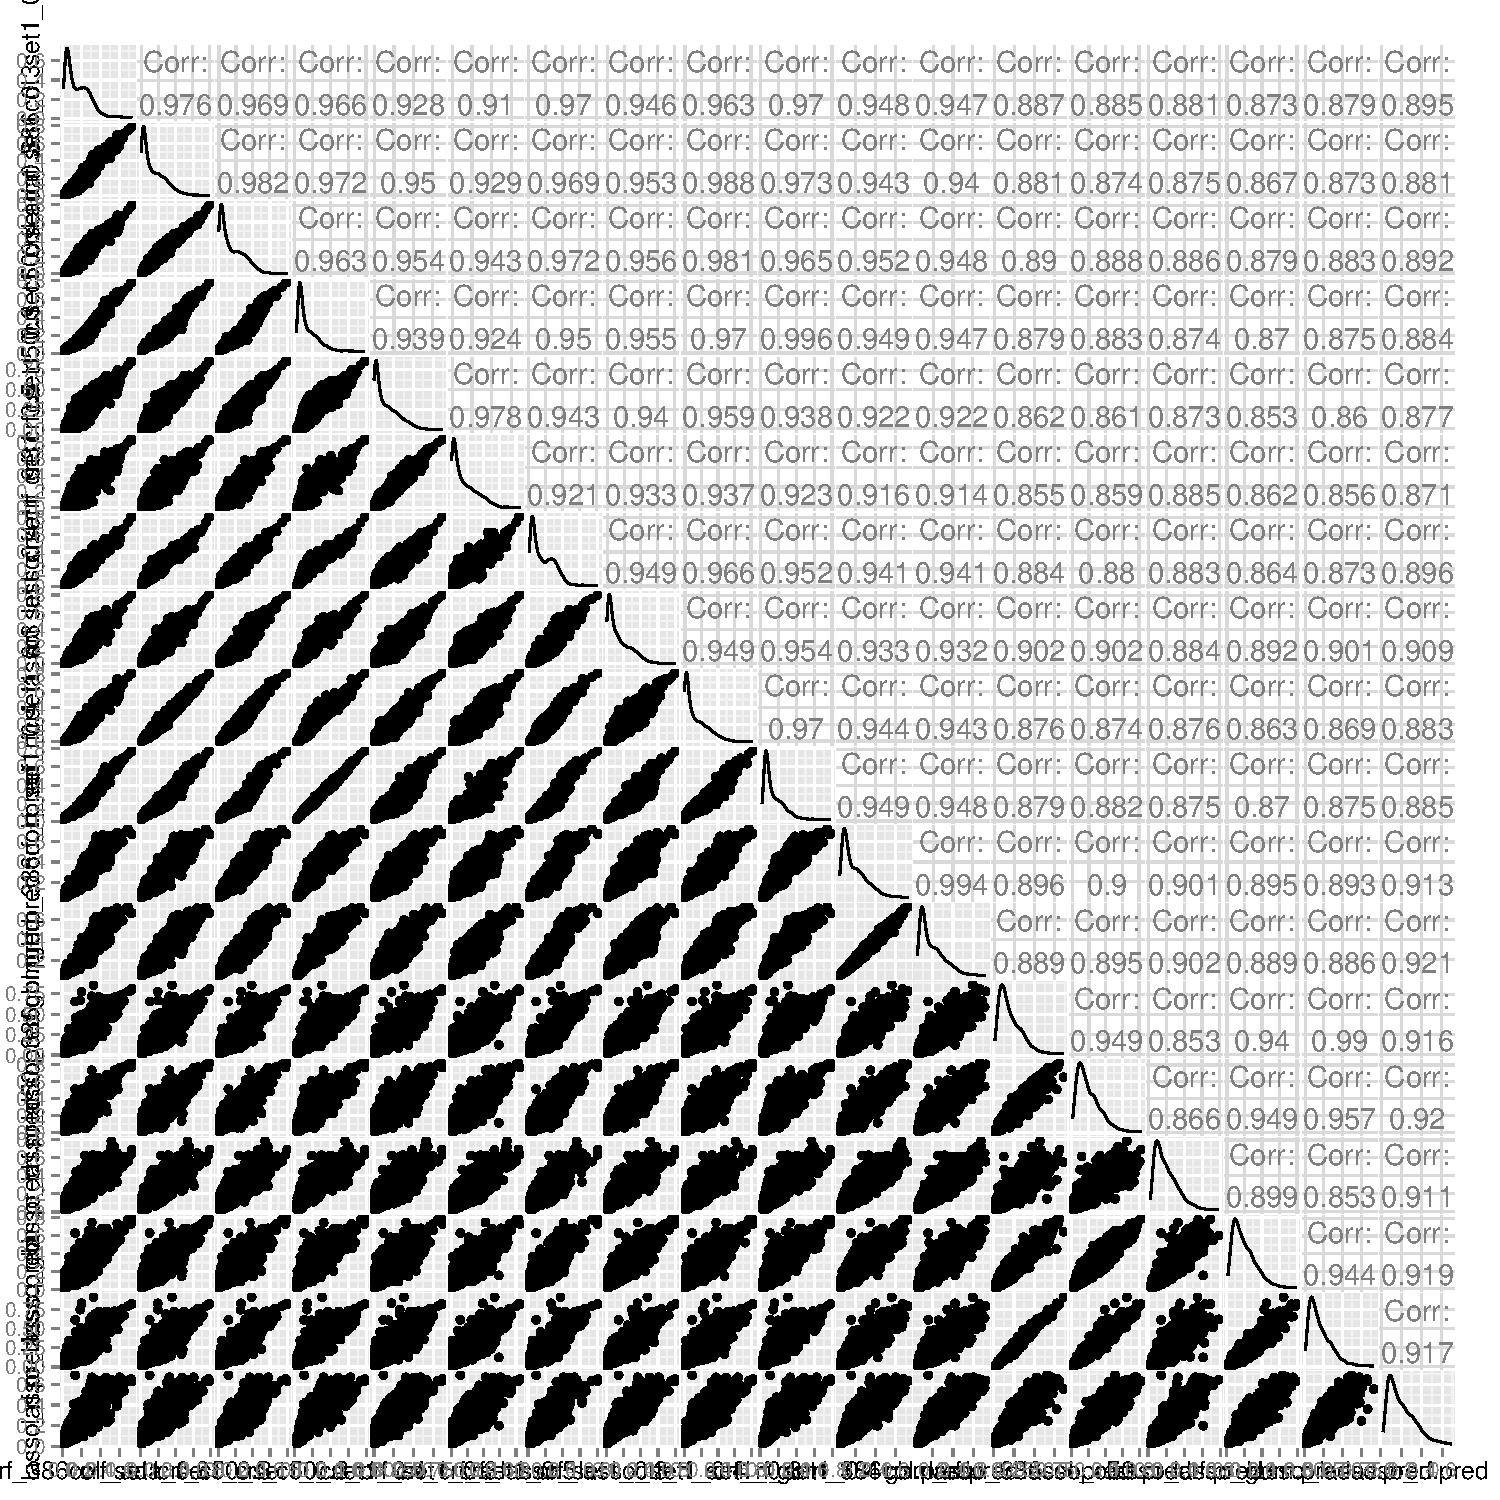
\includegraphics{/Users/user/dmc2015/ian/graphics/fig_unnamed-chunk-8-1} \end{center}

\subsection{Created Variables}\label{created-variables}

\emph{couponCol}

\begin{Shaded}
\begin{Highlighting}[]
\CommentTok{# couponCol}
\NormalTok{llr =}\StringTok{ }\KeywordTok{compute_ll}\NormalTok{(}\KeywordTok{as.character}\NormalTok{(H$couponCol), H$couponUsed, }\KeywordTok{as.character}\NormalTok{(TVC$couponCol))}
\NormalTok{llr_couponCol =}\StringTok{ }\KeywordTok{data.frame}\NormalTok{(}\DataTypeTok{couponCol =} \KeywordTok{names}\NormalTok{(llr), }\DataTypeTok{llr_couponCol =} \NormalTok{llr) %>%}\StringTok{ }
\StringTok{    }\KeywordTok{arrange}\NormalTok{(couponCol) %>%}\StringTok{ }\NormalTok{unique}
\NormalTok{llr_couponCol$couponCol =}\StringTok{ }\KeywordTok{as.character}\NormalTok{(llr_couponCol$couponCol)}

\CommentTok{# plot the results}
\NormalTok{if (}\KeywordTok{nrow}\NormalTok{(TVC) -}\StringTok{ }\KeywordTok{sum}\NormalTok{(TVC$couponCol %in%}\StringTok{ }\NormalTok{llr_couponCol$couponCol)) }\KeywordTok{warning}\NormalTok{(}\StringTok{"Things aren't adding up"}\NormalTok{)}
\KeywordTok{qplot}\NormalTok{(}\KeywordTok{as.numeric}\NormalTok{(}\KeywordTok{gsub}\NormalTok{(}\StringTok{"cpn"}\NormalTok{, }\StringTok{""}\NormalTok{, couponCol)), llr_couponCol, }\DataTypeTok{data =} \NormalTok{llr_couponCol)}

\CommentTok{# Isolate the features}
\NormalTok{llr_couponCol_long =}\StringTok{ }\NormalTok{TVC %>%}\StringTok{ }\KeywordTok{left_join}\NormalTok{(llr_couponCol, }\DataTypeTok{by =} \StringTok{"couponCol"}\NormalTok{) %>%}\StringTok{ }
\StringTok{    }\KeywordTok{arrange}\NormalTok{(orderID, couponCol) %>%}\StringTok{ }\KeywordTok{select}\NormalTok{(orderID, couponCol, dsn, llr_couponCol)}

\NormalTok{trn =}\StringTok{ }\NormalTok{llr_couponCol_long %>%}\StringTok{ }\KeywordTok{filter}\NormalTok{(dsn ==}\StringTok{ "train"}\NormalTok{) %>%}\StringTok{ }\KeywordTok{select}\NormalTok{(orderID, couponCol, }
    \NormalTok{llr_couponCol)}
\NormalTok{val =}\StringTok{ }\NormalTok{llr_couponCol_long %>%}\StringTok{ }\KeywordTok{filter}\NormalTok{(dsn ==}\StringTok{ "validation"}\NormalTok{) %>%}\StringTok{ }\KeywordTok{select}\NormalTok{(orderID, }
    \NormalTok{couponCol, llr_couponCol)}
\NormalTok{cls =}\StringTok{ }\NormalTok{llr_couponCol_long %>%}\StringTok{ }\KeywordTok{filter}\NormalTok{(dsn ==}\StringTok{ "class"}\NormalTok{) %>%}\StringTok{ }\KeywordTok{select}\NormalTok{(orderID, couponCol, }
    \NormalTok{llr_couponCol)}

\NormalTok{llr_couponCol_long =}\StringTok{ }\KeywordTok{list}\NormalTok{(}\DataTypeTok{T =} \NormalTok{trn, }\DataTypeTok{V =} \NormalTok{val, }\DataTypeTok{C =} \NormalTok{cls)}

\KeywordTok{saveRDS}\NormalTok{(llr_couponCol_long, }\StringTok{"../features/feature_files/llr_couponCol_long_set1.rds"}\NormalTok{)}

\CommentTok{# save the results to RDS in WIDE format}
\NormalTok{llr_couponCol_wide =}\StringTok{ }\NormalTok{TVC %>%}\StringTok{ }\KeywordTok{left_join}\NormalTok{(llr_couponCol, }\DataTypeTok{by =} \StringTok{"couponCol"}\NormalTok{) %>%}\StringTok{ }
\StringTok{    }\KeywordTok{arrange}\NormalTok{(orderID, couponCol) %>%}\StringTok{ }\KeywordTok{select}\NormalTok{(orderID, couponCol, dsn, llr_couponCol) %>%}\StringTok{ }
\StringTok{    }\KeywordTok{spread}\NormalTok{(couponCol, llr_couponCol) %>%}\StringTok{ }\KeywordTok{renm}\NormalTok{(}\KeywordTok{c}\NormalTok{(}\StringTok{"orderID"}\NormalTok{, }\StringTok{"dsn"}\NormalTok{, }\StringTok{"llr_couponCol1"}\NormalTok{, }
    \StringTok{"llr_couponCol2"}\NormalTok{, }\StringTok{"llr_couponCol3"}\NormalTok{))}

\NormalTok{trn =}\StringTok{ }\NormalTok{llr_couponCol_wide %>%}\StringTok{ }\KeywordTok{filter}\NormalTok{(dsn ==}\StringTok{ "train"}\NormalTok{) %>%}\StringTok{ }\KeywordTok{select}\NormalTok{(orderID, llr_couponCol1, }
    \NormalTok{llr_couponCol2, llr_couponCol3)}
\NormalTok{val =}\StringTok{ }\NormalTok{llr_couponCol_wide %>%}\StringTok{ }\KeywordTok{filter}\NormalTok{(dsn ==}\StringTok{ "validation"}\NormalTok{) %>%}\StringTok{ }\KeywordTok{select}\NormalTok{(orderID, }
    \NormalTok{llr_couponCol1, llr_couponCol2, llr_couponCol3)}
\NormalTok{cls =}\StringTok{ }\NormalTok{llr_couponCol_wide %>%}\StringTok{ }\KeywordTok{filter}\NormalTok{(dsn ==}\StringTok{ "class"}\NormalTok{) %>%}\StringTok{ }\KeywordTok{select}\NormalTok{(orderID, llr_couponCol1, }
    \NormalTok{llr_couponCol2, llr_couponCol3)}

\NormalTok{llr_couponCol_wide =}\StringTok{ }\KeywordTok{list}\NormalTok{(}\DataTypeTok{T =} \NormalTok{trn, }\DataTypeTok{V =} \NormalTok{val, }\DataTypeTok{C =} \NormalTok{cls)}

\KeywordTok{saveRDS}\NormalTok{(llr_couponCol_wide, }\StringTok{"../features/feature_files/llr_couponCol_wide.rds"}\NormalTok{)}
\end{Highlighting}
\end{Shaded}

\begin{center}\includegraphics{/Users/user/dmc2015/ian/graphics/fig_unnamed-chunk-9-1} \end{center}

\emph{couponsReceivedDoW}

\begin{Shaded}
\begin{Highlighting}[]
\CommentTok{# couponsReceivedDoW}
\NormalTok{llr =}\StringTok{ }\KeywordTok{compute_ll}\NormalTok{(}\KeywordTok{as.character}\NormalTok{(H$couponsReceivedDoW), H$couponUsed, }\KeywordTok{as.character}\NormalTok{(TVC$couponsReceivedDoW))}
\NormalTok{llr_couponsReceivedDoW =}\StringTok{ }\KeywordTok{data.frame}\NormalTok{(}\DataTypeTok{couponsReceivedDoW =} \KeywordTok{names}\NormalTok{(llr), }\DataTypeTok{llr_couponsReceivedDoW =} \NormalTok{llr) %>%}\StringTok{ }
\StringTok{    }\KeywordTok{arrange}\NormalTok{(couponsReceivedDoW) %>%}\StringTok{ }\NormalTok{unique}

\CommentTok{# plot the results}
\NormalTok{if (}\KeywordTok{nrow}\NormalTok{(TVC) -}\StringTok{ }\KeywordTok{sum}\NormalTok{(TVC$couponsReceivedDoW %in%}\StringTok{ }\NormalTok{llr_couponsReceivedDoW$couponsReceivedDoW)) }\KeywordTok{warning}\NormalTok{(}\StringTok{"Things aren't adding up"}\NormalTok{)}
\KeywordTok{qplot}\NormalTok{(couponsReceivedDoW, llr_couponsReceivedDoW, }\DataTypeTok{data =} \NormalTok{llr_couponsReceivedDoW)}

\CommentTok{# Isolate the features}
\NormalTok{llr_couponsReceivedDoW_long =}\StringTok{ }\NormalTok{TVC %>%}\StringTok{ }\KeywordTok{left_join}\NormalTok{(llr_couponsReceivedDoW, }\DataTypeTok{by =} \StringTok{"couponsReceivedDoW"}\NormalTok{) %>%}\StringTok{ }
\StringTok{    }\KeywordTok{arrange}\NormalTok{(orderID, couponsReceivedDoW) %>%}\StringTok{ }\KeywordTok{select}\NormalTok{(orderID, couponsReceivedDoW, }
    \NormalTok{dsn, llr_couponsReceivedDoW)}
\end{Highlighting}
\end{Shaded}

\begin{verbatim}
## Warning in left_join_impl(x, y, by$x, by$y): joining factors with
## different levels, coercing to character vector
\end{verbatim}

\begin{Shaded}
\begin{Highlighting}[]
\NormalTok{trn =}\StringTok{ }\NormalTok{llr_couponsReceivedDoW_long %>%}\StringTok{ }\KeywordTok{filter}\NormalTok{(dsn ==}\StringTok{ "train"}\NormalTok{) %>%}\StringTok{ }\KeywordTok{select}\NormalTok{(orderID, }
    \NormalTok{couponsReceivedDoW, llr_couponsReceivedDoW)}
\NormalTok{val =}\StringTok{ }\NormalTok{llr_couponsReceivedDoW_long %>%}\StringTok{ }\KeywordTok{filter}\NormalTok{(dsn ==}\StringTok{ "validation"}\NormalTok{) %>%}\StringTok{ }\KeywordTok{select}\NormalTok{(orderID, }
    \NormalTok{couponsReceivedDoW, llr_couponsReceivedDoW)}
\NormalTok{cls =}\StringTok{ }\NormalTok{llr_couponsReceivedDoW_long %>%}\StringTok{ }\KeywordTok{filter}\NormalTok{(dsn ==}\StringTok{ "class"}\NormalTok{) %>%}\StringTok{ }\KeywordTok{select}\NormalTok{(orderID, }
    \NormalTok{couponsReceivedDoW, llr_couponsReceivedDoW)}

\NormalTok{llr_couponsReceivedDoW_long =}\StringTok{ }\KeywordTok{list}\NormalTok{(}\DataTypeTok{T =} \NormalTok{trn, }\DataTypeTok{V =} \NormalTok{val, }\DataTypeTok{C =} \NormalTok{cls)}

\KeywordTok{saveRDS}\NormalTok{(llr_couponsReceivedDoW_long, }\StringTok{"../features/feature_files/llr_couponsReceivedDoW_long_set1.rds"}\NormalTok{)}

\CommentTok{# save the results to RDS in WIDE format}
\NormalTok{llr_couponsReceivedDoW_wide =}\StringTok{ }\NormalTok{TVC %>%}\StringTok{ }\KeywordTok{left_join}\NormalTok{(llr_couponsReceivedDoW, }\DataTypeTok{by =} \StringTok{"couponsReceivedDoW"}\NormalTok{) %>%}\StringTok{ }
\StringTok{    }\KeywordTok{arrange}\NormalTok{(orderID, couponCol) %>%}\StringTok{ }\KeywordTok{select}\NormalTok{(orderID, couponCol, dsn, llr_couponsReceivedDoW) %>%}\StringTok{ }
\StringTok{    }\KeywordTok{spread}\NormalTok{(couponCol, llr_couponsReceivedDoW) %>%}\StringTok{ }\KeywordTok{renm}\NormalTok{(}\KeywordTok{c}\NormalTok{(}\StringTok{"orderID"}\NormalTok{, }\StringTok{"dsn"}\NormalTok{, }\StringTok{"llr_couponsReceivedDoW1"}\NormalTok{, }
    \StringTok{"llr_couponsReceivedDoW2"}\NormalTok{, }\StringTok{"llr_couponsReceivedDoW3"}\NormalTok{))}
\end{Highlighting}
\end{Shaded}

\begin{verbatim}
## Warning in left_join_impl(x, y, by$x, by$y): joining factors with
## different levels, coercing to character vector
\end{verbatim}

\begin{Shaded}
\begin{Highlighting}[]
\NormalTok{trn =}\StringTok{ }\NormalTok{llr_couponsReceivedDoW_wide %>%}\StringTok{ }\KeywordTok{filter}\NormalTok{(dsn ==}\StringTok{ "train"}\NormalTok{) %>%}\StringTok{ }\KeywordTok{select}\NormalTok{(orderID, }
    \NormalTok{llr_couponsReceivedDoW1, llr_couponsReceivedDoW2, llr_couponsReceivedDoW3)}
\NormalTok{val =}\StringTok{ }\NormalTok{llr_couponsReceivedDoW_wide %>%}\StringTok{ }\KeywordTok{filter}\NormalTok{(dsn ==}\StringTok{ "validation"}\NormalTok{) %>%}\StringTok{ }\KeywordTok{select}\NormalTok{(orderID, }
    \NormalTok{llr_couponsReceivedDoW1, llr_couponsReceivedDoW2, llr_couponsReceivedDoW3)}
\NormalTok{cls =}\StringTok{ }\NormalTok{llr_couponsReceivedDoW_wide %>%}\StringTok{ }\KeywordTok{filter}\NormalTok{(dsn ==}\StringTok{ "class"}\NormalTok{) %>%}\StringTok{ }\KeywordTok{select}\NormalTok{(orderID, }
    \NormalTok{llr_couponsReceivedDoW1, llr_couponsReceivedDoW2, llr_couponsReceivedDoW3)}

\NormalTok{llr_couponsReceivedDoW_wide =}\StringTok{ }\KeywordTok{list}\NormalTok{(}\DataTypeTok{T =} \NormalTok{trn, }\DataTypeTok{V =} \NormalTok{val, }\DataTypeTok{C =} \NormalTok{cls)}

\KeywordTok{saveRDS}\NormalTok{(llr_couponsReceivedDoW_wide, }\StringTok{"../features/feature_files/llr_couponsReceivedDoW_wide.rds"}\NormalTok{)}
\end{Highlighting}
\end{Shaded}

\begin{center}\includegraphics{/Users/user/dmc2015/ian/graphics/fig_unnamed-chunk-10-1} \end{center}

\emph{orderTimeDoW}

\begin{Shaded}
\begin{Highlighting}[]
\CommentTok{# orderTimeDoW}
\NormalTok{llr =}\StringTok{ }\KeywordTok{compute_ll}\NormalTok{(}\KeywordTok{as.character}\NormalTok{(H$orderTimeDoW), H$couponUsed, }\KeywordTok{as.character}\NormalTok{(TVC$orderTimeDoW))}
\NormalTok{llr_orderTimeDoW =}\StringTok{ }\KeywordTok{data.frame}\NormalTok{(}\DataTypeTok{orderTimeDoW =} \KeywordTok{names}\NormalTok{(llr), }\DataTypeTok{llr_orderTimeDoW =} \NormalTok{llr) %>%}\StringTok{ }
\StringTok{    }\KeywordTok{arrange}\NormalTok{(orderTimeDoW) %>%}\StringTok{ }\NormalTok{unique}

\CommentTok{# plot the results}
\NormalTok{if (}\KeywordTok{nrow}\NormalTok{(TVC) -}\StringTok{ }\KeywordTok{sum}\NormalTok{(TVC$orderTimeDoW %in%}\StringTok{ }\NormalTok{llr_orderTimeDoW$orderTimeDoW)) }\KeywordTok{warning}\NormalTok{(}\StringTok{"Things aren't adding up"}\NormalTok{)}
\KeywordTok{qplot}\NormalTok{(orderTimeDoW, llr_orderTimeDoW, }\DataTypeTok{data =} \NormalTok{llr_orderTimeDoW)}

\CommentTok{# Isolate the features}
\NormalTok{llr_orderTimeDoW_long =}\StringTok{ }\NormalTok{TVC %>%}\StringTok{ }\KeywordTok{left_join}\NormalTok{(llr_orderTimeDoW, }\DataTypeTok{by =} \StringTok{"orderTimeDoW"}\NormalTok{) %>%}\StringTok{ }
\StringTok{    }\KeywordTok{arrange}\NormalTok{(orderID, orderTimeDoW) %>%}\StringTok{ }\KeywordTok{select}\NormalTok{(orderID, orderTimeDoW, dsn, llr_orderTimeDoW)}
\end{Highlighting}
\end{Shaded}

\begin{verbatim}
## Warning in left_join_impl(x, y, by$x, by$y): joining factors with
## different levels, coercing to character vector
\end{verbatim}

\begin{Shaded}
\begin{Highlighting}[]
\NormalTok{trn =}\StringTok{ }\NormalTok{llr_orderTimeDoW_long %>%}\StringTok{ }\KeywordTok{filter}\NormalTok{(dsn ==}\StringTok{ "train"}\NormalTok{) %>%}\StringTok{ }\KeywordTok{select}\NormalTok{(orderID, orderTimeDoW, }
    \NormalTok{llr_orderTimeDoW)}
\NormalTok{val =}\StringTok{ }\NormalTok{llr_orderTimeDoW_long %>%}\StringTok{ }\KeywordTok{filter}\NormalTok{(dsn ==}\StringTok{ "validation"}\NormalTok{) %>%}\StringTok{ }\KeywordTok{select}\NormalTok{(orderID, }
    \NormalTok{orderTimeDoW, llr_orderTimeDoW)}
\NormalTok{cls =}\StringTok{ }\NormalTok{llr_orderTimeDoW_long %>%}\StringTok{ }\KeywordTok{filter}\NormalTok{(dsn ==}\StringTok{ "class"}\NormalTok{) %>%}\StringTok{ }\KeywordTok{select}\NormalTok{(orderID, orderTimeDoW, }
    \NormalTok{llr_orderTimeDoW)}

\NormalTok{llr_orderTimeDoW_long =}\StringTok{ }\KeywordTok{list}\NormalTok{(}\DataTypeTok{T =} \NormalTok{trn, }\DataTypeTok{V =} \NormalTok{val, }\DataTypeTok{C =} \NormalTok{cls)}

\KeywordTok{saveRDS}\NormalTok{(llr_orderTimeDoW_long, }\StringTok{"../features/feature_files/llr_orderTimeDoW_long_set1.rds"}\NormalTok{)}

\CommentTok{# save the results to RDS in WIDE format}
\NormalTok{llr_orderTimeDoW_wide =}\StringTok{ }\NormalTok{TVC %>%}\StringTok{ }\KeywordTok{left_join}\NormalTok{(llr_orderTimeDoW, }\DataTypeTok{by =} \StringTok{"orderTimeDoW"}\NormalTok{) %>%}\StringTok{ }
\StringTok{    }\KeywordTok{arrange}\NormalTok{(orderID, couponCol) %>%}\StringTok{ }\KeywordTok{select}\NormalTok{(orderID, couponCol, dsn, llr_orderTimeDoW) %>%}\StringTok{ }
\StringTok{    }\KeywordTok{spread}\NormalTok{(couponCol, llr_orderTimeDoW) %>%}\StringTok{ }\KeywordTok{renm}\NormalTok{(}\KeywordTok{c}\NormalTok{(}\StringTok{"orderID"}\NormalTok{, }\StringTok{"dsn"}\NormalTok{, }\StringTok{"llr_orderTimeDoW1"}\NormalTok{, }
    \StringTok{"llr_orderTimeDoW2"}\NormalTok{, }\StringTok{"llr_orderTimeDoW3"}\NormalTok{))}
\end{Highlighting}
\end{Shaded}

\begin{verbatim}
## Warning in left_join_impl(x, y, by$x, by$y): joining factors with
## different levels, coercing to character vector
\end{verbatim}

\begin{Shaded}
\begin{Highlighting}[]
\NormalTok{trn =}\StringTok{ }\NormalTok{llr_orderTimeDoW_wide %>%}\StringTok{ }\KeywordTok{filter}\NormalTok{(dsn ==}\StringTok{ "train"}\NormalTok{) %>%}\StringTok{ }\KeywordTok{select}\NormalTok{(orderID, llr_orderTimeDoW1, }
    \NormalTok{llr_orderTimeDoW2, llr_orderTimeDoW3)}
\NormalTok{val =}\StringTok{ }\NormalTok{llr_orderTimeDoW_wide %>%}\StringTok{ }\KeywordTok{filter}\NormalTok{(dsn ==}\StringTok{ "validation"}\NormalTok{) %>%}\StringTok{ }\KeywordTok{select}\NormalTok{(orderID, }
    \NormalTok{llr_orderTimeDoW1, llr_orderTimeDoW2, llr_orderTimeDoW3)}
\NormalTok{cls =}\StringTok{ }\NormalTok{llr_orderTimeDoW_wide %>%}\StringTok{ }\KeywordTok{filter}\NormalTok{(dsn ==}\StringTok{ "class"}\NormalTok{) %>%}\StringTok{ }\KeywordTok{select}\NormalTok{(orderID, llr_orderTimeDoW1, }
    \NormalTok{llr_orderTimeDoW2, llr_orderTimeDoW3)}

\NormalTok{llr_orderTimeDoW_wide =}\StringTok{ }\KeywordTok{list}\NormalTok{(}\DataTypeTok{T =} \NormalTok{trn, }\DataTypeTok{V =} \NormalTok{val, }\DataTypeTok{C =} \NormalTok{cls)}

\KeywordTok{saveRDS}\NormalTok{(llr_orderTimeDoW_wide, }\StringTok{"../features/feature_files/llr_orderTimeDoW_wide.rds"}\NormalTok{)}
\end{Highlighting}
\end{Shaded}

\begin{center}\includegraphics{/Users/user/dmc2015/ian/graphics/fig_unnamed-chunk-11-1} \end{center}

\section{Calculating Coupon 2-Way
Likelihoods}\label{calculating-coupon-2-way-likelihoods}

We have a sligthly more complicated task on this one:

\begin{Shaded}
\begin{Highlighting}[]
\KeywordTok{names}\NormalTok{(TVC)[-}\KeywordTok{c}\NormalTok{(}\DecValTok{1}\NormalTok{, }\DecValTok{2}\NormalTok{, }\DecValTok{4}\NormalTok{, }\DecValTok{5}\NormalTok{, }\DecValTok{6}\NormalTok{, }\DecValTok{7}\NormalTok{, }\DecValTok{11}\NormalTok{, }\DecValTok{12}\NormalTok{, }\DecValTok{16}\NormalTok{, }\DecValTok{17}\NormalTok{:}\DecValTok{22}\NormalTok{, }\DecValTok{24}\NormalTok{:}\DecValTok{25}\NormalTok{, }\DecValTok{31}\NormalTok{)]}
\end{Highlighting}
\end{Shaded}

\begin{verbatim}
##  [1] "userID"                 "couponsReceivedDoW"    
##  [3] "couponsReceivedWeekend" "couponsReceivedFriSat" 
##  [5] "orderTimeDoW"           "orderTimeWeekend"      
##  [7] "orderTimeFriSat"        "dsn"                   
##  [9] "basePrice"              "reward"                
## [11] "premiumProduct"         "brand"                 
## [13] "productGroup"           "couponUsed"            
## [15] "couponCol"
\end{verbatim}

\begin{Shaded}
\begin{Highlighting}[]
\KeywordTok{names}\NormalTok{(TVC)}
\end{Highlighting}
\end{Shaded}

\begin{verbatim}
##  [1] "orderID"                "orderTime"             
##  [3] "userID"                 "couponsReceived"       
##  [5] "basketValue"            "couponsReceivedDate"   
##  [7] "couponsReceivedTime"    "couponsReceivedDoW"    
##  [9] "couponsReceivedWeekend" "couponsReceivedFriSat" 
## [11] "orderTimeDate"          "orderTimeTime"         
## [13] "orderTimeDoW"           "orderTimeWeekend"      
## [15] "orderTimeFriSat"        "batchID"               
## [17] "couponsExpire"          "couponsSent"           
## [19] "TimeBtwnSentRec"        "TimeBtwnRecExpire"     
## [21] "TimeBtwnRecOrder"       "TimeBtwnOrderExpire"   
## [23] "dsn"                    "couponID"              
## [25] "price"                  "basePrice"             
## [27] "reward"                 "premiumProduct"        
## [29] "brand"                  "productGroup"          
## [31] "categoryIDs"            "couponUsed"            
## [33] "couponCol"
\end{verbatim}

\subsection{userID and}\label{userid-and}

\emph{couponsReceivedDoW} (as \texttt{llr\_userXrecDoW})

\begin{Shaded}
\begin{Highlighting}[]
\CommentTok{# couponsReceivedDoW}
\NormalTok{llr =}\StringTok{ }\KeywordTok{compute_ll_2w}\NormalTok{(}\KeywordTok{as.character}\NormalTok{(H$userID), }\KeywordTok{as.character}\NormalTok{(H$couponsReceivedDoW), }
    \NormalTok{H$couponUsed, }\KeywordTok{as.character}\NormalTok{(TVC$userID), }\KeywordTok{as.character}\NormalTok{(TVC$couponsReceivedDoW))}
\NormalTok{llr_userXrecDoW =}\StringTok{ }\KeywordTok{data.frame}\NormalTok{(}\DataTypeTok{userID =} \NormalTok{TVC$userID, }\DataTypeTok{couponsReceivedDoW =} \NormalTok{TVC$couponsReceivedDoW, }
    \DataTypeTok{llr_userXrecDoW =} \NormalTok{llr) %>%}\StringTok{ }\KeywordTok{arrange}\NormalTok{(userID)}

\KeywordTok{ggplot}\NormalTok{(}\DataTypeTok{data =} \NormalTok{llr_userXrecDoW, }\KeywordTok{aes}\NormalTok{(}\DataTypeTok{x =} \NormalTok{userID, }\DataTypeTok{y =} \NormalTok{couponsReceivedDoW, }\DataTypeTok{size =} \NormalTok{llr_userXrecDoW), }
    \DataTypeTok{alpha =} \FloatTok{0.1}\NormalTok{) +}\StringTok{ }\KeywordTok{geom_point}\NormalTok{()}
\KeywordTok{qplot}\NormalTok{(userID, llr_userXrecDoW, }\DataTypeTok{data =} \NormalTok{llr_userXrecDoW, }\DataTypeTok{geom =} \StringTok{"line"}\NormalTok{, }\DataTypeTok{group =} \NormalTok{couponsReceivedDoW, }
    \DataTypeTok{facets =} \NormalTok{couponsReceivedDoW ~}\StringTok{ }\NormalTok{.)}

\NormalTok{TVC %>%}\StringTok{ }\KeywordTok{left_join}\NormalTok{(llr_userXrecDoW, }\DataTypeTok{by =} \KeywordTok{c}\NormalTok{(}\StringTok{"userID"}\NormalTok{, }\StringTok{"couponsReceivedDoW"}\NormalTok{)) %>%}\StringTok{ }
\StringTok{    }\KeywordTok{select}\NormalTok{(orderID, userID, dsn, couponsReceivedDoW, llr_userXrecDoW, couponUsed) %>%}\StringTok{ }
\StringTok{    }\KeywordTok{ggplot}\NormalTok{(}\KeywordTok{aes}\NormalTok{(}\DataTypeTok{x =} \NormalTok{couponsReceivedDoW, }\DataTypeTok{y =} \NormalTok{llr_userXrecDoW, }\DataTypeTok{fill =} \KeywordTok{factor}\NormalTok{(couponUsed), }
        \DataTypeTok{color =} \NormalTok{dsn)) +}\StringTok{ }\KeywordTok{geom_boxplot}\NormalTok{() +}\StringTok{ }\KeywordTok{facet_grid}\NormalTok{(dsn ~}\StringTok{ }\NormalTok{.)}
\end{Highlighting}
\end{Shaded}

\begin{verbatim}
## Warning in left_join_impl(x, y, by$x, by$y): joining factor and character
## vector, coercing into character vector
\end{verbatim}

\begin{Shaded}
\begin{Highlighting}[]
\NormalTok{llr_userXrecDoW =}\StringTok{ }\NormalTok{TVC %>%}\StringTok{ }\KeywordTok{left_join}\NormalTok{(llr_userXrecDoW, }\DataTypeTok{by =} \KeywordTok{c}\NormalTok{(}\StringTok{"userID"}\NormalTok{, }\StringTok{"couponsReceivedDoW"}\NormalTok{)) %>%}\StringTok{ }
\StringTok{    }\KeywordTok{select}\NormalTok{(orderID, dsn, llr_userXrecDoW)}
\end{Highlighting}
\end{Shaded}

\begin{verbatim}
## Warning in left_join_impl(x, y, by$x, by$y): joining factor and character
## vector, coercing into character vector
\end{verbatim}

\begin{Shaded}
\begin{Highlighting}[]
\NormalTok{trn =}\StringTok{ }\NormalTok{llr_userXrecDoW %>%}\StringTok{ }\KeywordTok{filter}\NormalTok{(dsn ==}\StringTok{ "train"}\NormalTok{) %>%}\StringTok{ }\KeywordTok{select}\NormalTok{(-dsn)}
\NormalTok{val =}\StringTok{ }\NormalTok{llr_userXrecDoW %>%}\StringTok{ }\KeywordTok{filter}\NormalTok{(dsn ==}\StringTok{ "validation"}\NormalTok{) %>%}\StringTok{ }\KeywordTok{select}\NormalTok{(-dsn)}
\NormalTok{cls =}\StringTok{ }\NormalTok{llr_userXrecDoW %>%}\StringTok{ }\KeywordTok{filter}\NormalTok{(dsn ==}\StringTok{ "class"}\NormalTok{) %>%}\StringTok{ }\KeywordTok{select}\NormalTok{(-dsn)}

\NormalTok{llr_userXrecDoW =}\StringTok{ }\KeywordTok{list}\NormalTok{(}\DataTypeTok{T =} \NormalTok{trn, }\DataTypeTok{V =} \NormalTok{val, }\DataTypeTok{C =} \NormalTok{cls)}

\KeywordTok{saveRDS}\NormalTok{(llr_userXrecDoW, }\StringTok{"../features/feature_files/llr_userXrecDoW.rds"}\NormalTok{)}
\end{Highlighting}
\end{Shaded}

\begin{center}\includegraphics{/Users/user/dmc2015/ian/graphics/fig_unnamed-chunk-12-1} \includegraphics{/Users/user/dmc2015/ian/graphics/fig_unnamed-chunk-12-2} \includegraphics{/Users/user/dmc2015/ian/graphics/fig_unnamed-chunk-12-3} \end{center}

\emph{couponsReceivedFriSat} (as \texttt{llr\_userXrecFS})

\begin{Shaded}
\begin{Highlighting}[]
\CommentTok{# couponsReceivedFriSat}
\NormalTok{llr =}\StringTok{ }\KeywordTok{compute_ll_2w}\NormalTok{(}\KeywordTok{as.character}\NormalTok{(H$userID), }\KeywordTok{as.character}\NormalTok{(H$couponsReceivedFriSat), }
    \NormalTok{H$couponUsed, }\KeywordTok{as.character}\NormalTok{(TVC$userID), }\KeywordTok{as.character}\NormalTok{(TVC$couponsReceivedFriSat))}
\NormalTok{llr_userXrecFS =}\StringTok{ }\KeywordTok{data.frame}\NormalTok{(}\DataTypeTok{userID =} \NormalTok{TVC$userID, }\DataTypeTok{couponsReceivedFriSat =} \NormalTok{TVC$couponsReceivedFriSat, }
    \DataTypeTok{llr_userXrecFS =} \NormalTok{llr) %>%}\StringTok{ }\KeywordTok{arrange}\NormalTok{(userID)}

\KeywordTok{ggplot}\NormalTok{(}\DataTypeTok{data =} \NormalTok{llr_userXrecFS, }\KeywordTok{aes}\NormalTok{(}\DataTypeTok{x =} \NormalTok{userID, }\DataTypeTok{y =} \NormalTok{couponsReceivedFriSat, }\DataTypeTok{size =} \NormalTok{llr_userXrecFS), }
    \DataTypeTok{alpha =} \FloatTok{0.1}\NormalTok{) +}\StringTok{ }\KeywordTok{geom_point}\NormalTok{()}
\KeywordTok{qplot}\NormalTok{(userID, llr_userXrecFS, }\DataTypeTok{data =} \NormalTok{llr_userXrecFS, }\DataTypeTok{geom =} \StringTok{"line"}\NormalTok{, }\DataTypeTok{group =} \NormalTok{couponsReceivedFriSat, }
    \DataTypeTok{facets =} \NormalTok{couponsReceivedFriSat ~}\StringTok{ }\NormalTok{.)}

\NormalTok{TVC %>%}\StringTok{ }\KeywordTok{left_join}\NormalTok{(llr_userXrecFS, }\DataTypeTok{by =} \KeywordTok{c}\NormalTok{(}\StringTok{"userID"}\NormalTok{, }\StringTok{"couponsReceivedFriSat"}\NormalTok{)) %>%}\StringTok{ }
\StringTok{    }\KeywordTok{select}\NormalTok{(orderID, userID, dsn, couponsReceivedFriSat, llr_userXrecFS, couponUsed) %>%}\StringTok{ }
\StringTok{    }\KeywordTok{ggplot}\NormalTok{(}\KeywordTok{aes}\NormalTok{(}\DataTypeTok{x =} \NormalTok{couponsReceivedFriSat, }\DataTypeTok{y =} \NormalTok{llr_userXrecFS, }\DataTypeTok{fill =} \KeywordTok{factor}\NormalTok{(couponUsed), }
        \DataTypeTok{color =} \NormalTok{dsn)) +}\StringTok{ }\KeywordTok{geom_boxplot}\NormalTok{() +}\StringTok{ }\KeywordTok{facet_grid}\NormalTok{(dsn ~}\StringTok{ }\NormalTok{.)}
\end{Highlighting}
\end{Shaded}

\begin{verbatim}
## Warning in left_join_impl(x, y, by$x, by$y): joining factor and character
## vector, coercing into character vector
\end{verbatim}

\begin{Shaded}
\begin{Highlighting}[]
\NormalTok{llr_userXrecFS =}\StringTok{ }\NormalTok{TVC %>%}\StringTok{ }\KeywordTok{left_join}\NormalTok{(llr_userXrecFS, }\DataTypeTok{by =} \KeywordTok{c}\NormalTok{(}\StringTok{"userID"}\NormalTok{, }\StringTok{"couponsReceivedFriSat"}\NormalTok{)) %>%}\StringTok{ }
\StringTok{    }\KeywordTok{select}\NormalTok{(orderID, dsn, llr_userXrecFS)}
\end{Highlighting}
\end{Shaded}

\begin{verbatim}
## Warning in left_join_impl(x, y, by$x, by$y): joining factor and character
## vector, coercing into character vector
\end{verbatim}

\begin{Shaded}
\begin{Highlighting}[]
\NormalTok{trn =}\StringTok{ }\NormalTok{llr_userXrecFS %>%}\StringTok{ }\KeywordTok{filter}\NormalTok{(dsn ==}\StringTok{ "train"}\NormalTok{) %>%}\StringTok{ }\KeywordTok{select}\NormalTok{(-dsn)}
\NormalTok{val =}\StringTok{ }\NormalTok{llr_userXrecFS %>%}\StringTok{ }\KeywordTok{filter}\NormalTok{(dsn ==}\StringTok{ "validation"}\NormalTok{) %>%}\StringTok{ }\KeywordTok{select}\NormalTok{(-dsn)}
\NormalTok{cls =}\StringTok{ }\NormalTok{llr_userXrecFS %>%}\StringTok{ }\KeywordTok{filter}\NormalTok{(dsn ==}\StringTok{ "class"}\NormalTok{) %>%}\StringTok{ }\KeywordTok{select}\NormalTok{(-dsn)}

\NormalTok{llr_userXrecFS =}\StringTok{ }\KeywordTok{list}\NormalTok{(}\DataTypeTok{T =} \NormalTok{trn, }\DataTypeTok{V =} \NormalTok{val, }\DataTypeTok{C =} \NormalTok{cls)}

\KeywordTok{saveRDS}\NormalTok{(llr_userXrecFS, }\StringTok{"../features/feature_files/llr_userXrecFS.rds"}\NormalTok{)}
\end{Highlighting}
\end{Shaded}

\begin{center}\includegraphics{/Users/user/dmc2015/ian/graphics/fig_unnamed-chunk-13-1} \includegraphics{/Users/user/dmc2015/ian/graphics/fig_unnamed-chunk-13-2} \includegraphics{/Users/user/dmc2015/ian/graphics/fig_unnamed-chunk-13-3} \end{center}

\emph{couponsReceivedWeekend} (as \texttt{llr\_userXrecWknd})

\begin{Shaded}
\begin{Highlighting}[]
\CommentTok{# couponsReceivedWeekend}
\NormalTok{llr =}\StringTok{ }\KeywordTok{compute_ll_2w}\NormalTok{(}\KeywordTok{as.character}\NormalTok{(H$userID), }\KeywordTok{as.character}\NormalTok{(H$couponsReceivedWeekend), }
    \NormalTok{H$couponUsed, }\KeywordTok{as.character}\NormalTok{(TVC$userID), }\KeywordTok{as.character}\NormalTok{(TVC$couponsReceivedWeekend))}
\NormalTok{llr_userXrecWknd =}\StringTok{ }\KeywordTok{data.frame}\NormalTok{(}\DataTypeTok{userID =} \NormalTok{TVC$userID, }\DataTypeTok{couponsReceivedWeekend =} \NormalTok{TVC$couponsReceivedWeekend, }
    \DataTypeTok{llr_userXrecWknd =} \NormalTok{llr) %>%}\StringTok{ }\KeywordTok{arrange}\NormalTok{(userID)}

\KeywordTok{ggplot}\NormalTok{(}\DataTypeTok{data =} \NormalTok{llr_userXrecWknd, }\KeywordTok{aes}\NormalTok{(}\DataTypeTok{x =} \NormalTok{userID, }\DataTypeTok{y =} \NormalTok{couponsReceivedWeekend, }
    \DataTypeTok{size =} \NormalTok{llr_userXrecWknd), }\DataTypeTok{alpha =} \FloatTok{0.1}\NormalTok{) +}\StringTok{ }\KeywordTok{geom_point}\NormalTok{()}
\KeywordTok{qplot}\NormalTok{(userID, llr_userXrecWknd, }\DataTypeTok{data =} \NormalTok{llr_userXrecWknd, }\DataTypeTok{geom =} \StringTok{"line"}\NormalTok{, }\DataTypeTok{group =} \NormalTok{couponsReceivedWeekend, }
    \DataTypeTok{facets =} \NormalTok{couponsReceivedWeekend ~}\StringTok{ }\NormalTok{.)}

\NormalTok{TVC %>%}\StringTok{ }\KeywordTok{left_join}\NormalTok{(llr_userXrecWknd, }\DataTypeTok{by =} \KeywordTok{c}\NormalTok{(}\StringTok{"userID"}\NormalTok{, }\StringTok{"couponsReceivedWeekend"}\NormalTok{)) %>%}\StringTok{ }
\StringTok{    }\KeywordTok{select}\NormalTok{(orderID, userID, dsn, couponsReceivedWeekend, llr_userXrecWknd, couponUsed) %>%}\StringTok{ }
\StringTok{    }\KeywordTok{ggplot}\NormalTok{(}\KeywordTok{aes}\NormalTok{(}\DataTypeTok{x =} \NormalTok{couponsReceivedWeekend, }\DataTypeTok{y =} \NormalTok{llr_userXrecWknd, }\DataTypeTok{fill =} \KeywordTok{factor}\NormalTok{(couponUsed), }
        \DataTypeTok{color =} \NormalTok{dsn)) +}\StringTok{ }\KeywordTok{geom_boxplot}\NormalTok{() +}\StringTok{ }\KeywordTok{facet_grid}\NormalTok{(dsn ~}\StringTok{ }\NormalTok{.)}
\end{Highlighting}
\end{Shaded}

\begin{verbatim}
## Warning in left_join_impl(x, y, by$x, by$y): joining factor and character
## vector, coercing into character vector
\end{verbatim}

\begin{Shaded}
\begin{Highlighting}[]
\NormalTok{llr_userXrecWknd =}\StringTok{ }\NormalTok{TVC %>%}\StringTok{ }\KeywordTok{left_join}\NormalTok{(llr_userXrecWknd, }\DataTypeTok{by =} \KeywordTok{c}\NormalTok{(}\StringTok{"userID"}\NormalTok{, }\StringTok{"couponsReceivedWeekend"}\NormalTok{)) %>%}\StringTok{ }
\StringTok{    }\KeywordTok{select}\NormalTok{(orderID, dsn, llr_userXrecWknd)}
\end{Highlighting}
\end{Shaded}

\begin{verbatim}
## Warning in left_join_impl(x, y, by$x, by$y): joining factor and character
## vector, coercing into character vector
\end{verbatim}

\begin{Shaded}
\begin{Highlighting}[]
\NormalTok{trn =}\StringTok{ }\NormalTok{llr_userXrecWknd %>%}\StringTok{ }\KeywordTok{filter}\NormalTok{(dsn ==}\StringTok{ "train"}\NormalTok{) %>%}\StringTok{ }\KeywordTok{select}\NormalTok{(-dsn)}
\NormalTok{val =}\StringTok{ }\NormalTok{llr_userXrecWknd %>%}\StringTok{ }\KeywordTok{filter}\NormalTok{(dsn ==}\StringTok{ "validation"}\NormalTok{) %>%}\StringTok{ }\KeywordTok{select}\NormalTok{(-dsn)}
\NormalTok{cls =}\StringTok{ }\NormalTok{llr_userXrecWknd %>%}\StringTok{ }\KeywordTok{filter}\NormalTok{(dsn ==}\StringTok{ "class"}\NormalTok{) %>%}\StringTok{ }\KeywordTok{select}\NormalTok{(-dsn)}

\NormalTok{llr_userXrecWknd =}\StringTok{ }\KeywordTok{list}\NormalTok{(}\DataTypeTok{T =} \NormalTok{trn, }\DataTypeTok{V =} \NormalTok{val, }\DataTypeTok{C =} \NormalTok{cls)}

\KeywordTok{saveRDS}\NormalTok{(llr_userXrecWknd, }\StringTok{"../features/feature_files/llr_userXrecWknd.rds"}\NormalTok{)}
\end{Highlighting}
\end{Shaded}

\begin{center}\includegraphics{/Users/user/dmc2015/ian/graphics/fig_unnamed-chunk-14-1} \includegraphics{/Users/user/dmc2015/ian/graphics/fig_unnamed-chunk-14-2} \includegraphics{/Users/user/dmc2015/ian/graphics/fig_unnamed-chunk-14-3} \end{center}

\emph{orderTimeDoW} (as \texttt{llr\_userXordDoW})

\begin{Shaded}
\begin{Highlighting}[]
\CommentTok{# orderTimeDoW}
\NormalTok{llr =}\StringTok{ }\KeywordTok{compute_ll_2w}\NormalTok{(}\KeywordTok{as.character}\NormalTok{(H$userID), }\KeywordTok{as.character}\NormalTok{(H$orderTimeDoW), H$couponUsed, }
    \KeywordTok{as.character}\NormalTok{(TVC$userID), }\KeywordTok{as.character}\NormalTok{(TVC$orderTimeDoW))}
\NormalTok{llr_userXordDoW =}\StringTok{ }\KeywordTok{data.frame}\NormalTok{(}\DataTypeTok{userID =} \NormalTok{TVC$userID, }\DataTypeTok{orderTimeDoW =} \NormalTok{TVC$orderTimeDoW, }
    \DataTypeTok{llr_userXordDoW =} \NormalTok{llr) %>%}\StringTok{ }\KeywordTok{arrange}\NormalTok{(userID)}

\KeywordTok{ggplot}\NormalTok{(}\DataTypeTok{data =} \NormalTok{llr_userXordDoW, }\KeywordTok{aes}\NormalTok{(}\DataTypeTok{x =} \NormalTok{userID, }\DataTypeTok{y =} \NormalTok{orderTimeDoW, }\DataTypeTok{size =} \NormalTok{llr_userXordDoW), }
    \DataTypeTok{alpha =} \FloatTok{0.1}\NormalTok{) +}\StringTok{ }\KeywordTok{geom_point}\NormalTok{()}
\KeywordTok{qplot}\NormalTok{(userID, llr_userXordDoW, }\DataTypeTok{data =} \NormalTok{llr_userXordDoW, }\DataTypeTok{geom =} \StringTok{"line"}\NormalTok{, }\DataTypeTok{group =} \NormalTok{orderTimeDoW, }
    \DataTypeTok{facets =} \NormalTok{orderTimeDoW ~}\StringTok{ }\NormalTok{.)}

\NormalTok{TVC %>%}\StringTok{ }\KeywordTok{left_join}\NormalTok{(llr_userXordDoW, }\DataTypeTok{by =} \KeywordTok{c}\NormalTok{(}\StringTok{"userID"}\NormalTok{, }\StringTok{"orderTimeDoW"}\NormalTok{)) %>%}\StringTok{ }\KeywordTok{select}\NormalTok{(orderID, }
    \NormalTok{userID, dsn, orderTimeDoW, llr_userXordDoW, couponUsed) %>%}\StringTok{ }\KeywordTok{ggplot}\NormalTok{(}\KeywordTok{aes}\NormalTok{(}\DataTypeTok{x =} \NormalTok{orderTimeDoW, }
    \DataTypeTok{y =} \NormalTok{llr_userXordDoW, }\DataTypeTok{fill =} \KeywordTok{factor}\NormalTok{(couponUsed), }\DataTypeTok{color =} \NormalTok{dsn)) +}\StringTok{ }\KeywordTok{geom_boxplot}\NormalTok{() +}\StringTok{ }
\StringTok{    }\KeywordTok{facet_grid}\NormalTok{(dsn ~}\StringTok{ }\NormalTok{.)}
\end{Highlighting}
\end{Shaded}

\begin{verbatim}
## Warning in left_join_impl(x, y, by$x, by$y): joining factor and character
## vector, coercing into character vector
\end{verbatim}

\begin{Shaded}
\begin{Highlighting}[]
\NormalTok{llr_userXordDoW =}\StringTok{ }\NormalTok{TVC %>%}\StringTok{ }\KeywordTok{left_join}\NormalTok{(llr_userXordDoW, }\DataTypeTok{by =} \KeywordTok{c}\NormalTok{(}\StringTok{"userID"}\NormalTok{, }\StringTok{"orderTimeDoW"}\NormalTok{)) %>%}\StringTok{ }
\StringTok{    }\KeywordTok{select}\NormalTok{(orderID, dsn, llr_userXordDoW)}
\end{Highlighting}
\end{Shaded}

\begin{verbatim}
## Warning in left_join_impl(x, y, by$x, by$y): joining factor and character
## vector, coercing into character vector
\end{verbatim}

\begin{Shaded}
\begin{Highlighting}[]
\NormalTok{trn =}\StringTok{ }\NormalTok{llr_userXordDoW %>%}\StringTok{ }\KeywordTok{filter}\NormalTok{(dsn ==}\StringTok{ "train"}\NormalTok{) %>%}\StringTok{ }\KeywordTok{select}\NormalTok{(-dsn)}
\NormalTok{val =}\StringTok{ }\NormalTok{llr_userXordDoW %>%}\StringTok{ }\KeywordTok{filter}\NormalTok{(dsn ==}\StringTok{ "validation"}\NormalTok{) %>%}\StringTok{ }\KeywordTok{select}\NormalTok{(-dsn)}
\NormalTok{cls =}\StringTok{ }\NormalTok{llr_userXordDoW %>%}\StringTok{ }\KeywordTok{filter}\NormalTok{(dsn ==}\StringTok{ "class"}\NormalTok{) %>%}\StringTok{ }\KeywordTok{select}\NormalTok{(-dsn)}

\NormalTok{llr_userXordDoW =}\StringTok{ }\KeywordTok{list}\NormalTok{(}\DataTypeTok{T =} \NormalTok{trn, }\DataTypeTok{V =} \NormalTok{val, }\DataTypeTok{C =} \NormalTok{cls)}

\KeywordTok{saveRDS}\NormalTok{(llr_userXordDoW, }\StringTok{"../features/feature_files/llr_userXordDoW.rds"}\NormalTok{)}
\end{Highlighting}
\end{Shaded}

\begin{center}\includegraphics{/Users/user/dmc2015/ian/graphics/fig_unnamed-chunk-15-1} \includegraphics{/Users/user/dmc2015/ian/graphics/fig_unnamed-chunk-15-2} \includegraphics{/Users/user/dmc2015/ian/graphics/fig_unnamed-chunk-15-3} \end{center}

\emph{orderTimeFriSat} (as \texttt{llr\_userXordFS})

\begin{Shaded}
\begin{Highlighting}[]
\CommentTok{# orderTimeFriSat}
\NormalTok{llr =}\StringTok{ }\KeywordTok{compute_ll_2w}\NormalTok{(}\KeywordTok{as.character}\NormalTok{(H$userID), }\KeywordTok{as.character}\NormalTok{(H$orderTimeFriSat), }
    \NormalTok{H$couponUsed, }\KeywordTok{as.character}\NormalTok{(TVC$userID), }\KeywordTok{as.character}\NormalTok{(TVC$orderTimeFriSat))}
\NormalTok{llr_userXordFS =}\StringTok{ }\KeywordTok{data.frame}\NormalTok{(}\DataTypeTok{userID =} \NormalTok{TVC$userID, }\DataTypeTok{orderTimeFriSat =} \NormalTok{TVC$orderTimeFriSat, }
    \DataTypeTok{llr_userXordFS =} \NormalTok{llr) %>%}\StringTok{ }\KeywordTok{arrange}\NormalTok{(userID)}

\KeywordTok{ggplot}\NormalTok{(}\DataTypeTok{data =} \NormalTok{llr_userXordFS, }\KeywordTok{aes}\NormalTok{(}\DataTypeTok{x =} \NormalTok{userID, }\DataTypeTok{y =} \NormalTok{orderTimeFriSat, }\DataTypeTok{size =} \NormalTok{llr_userXordFS), }
    \DataTypeTok{alpha =} \FloatTok{0.1}\NormalTok{) +}\StringTok{ }\KeywordTok{geom_point}\NormalTok{()}
\KeywordTok{qplot}\NormalTok{(userID, llr_userXordFS, }\DataTypeTok{data =} \NormalTok{llr_userXordFS, }\DataTypeTok{geom =} \StringTok{"line"}\NormalTok{, }\DataTypeTok{group =} \NormalTok{orderTimeFriSat, }
    \DataTypeTok{facets =} \NormalTok{orderTimeFriSat ~}\StringTok{ }\NormalTok{.)}

\NormalTok{TVC %>%}\StringTok{ }\KeywordTok{left_join}\NormalTok{(llr_userXordFS, }\DataTypeTok{by =} \KeywordTok{c}\NormalTok{(}\StringTok{"userID"}\NormalTok{, }\StringTok{"orderTimeFriSat"}\NormalTok{)) %>%}\StringTok{ }\KeywordTok{select}\NormalTok{(orderID, }
    \NormalTok{userID, dsn, orderTimeFriSat, llr_userXordFS, couponUsed) %>%}\StringTok{ }\KeywordTok{ggplot}\NormalTok{(}\KeywordTok{aes}\NormalTok{(}\DataTypeTok{x =} \NormalTok{orderTimeFriSat, }
    \DataTypeTok{y =} \NormalTok{llr_userXordFS, }\DataTypeTok{fill =} \KeywordTok{factor}\NormalTok{(couponUsed), }\DataTypeTok{color =} \NormalTok{dsn)) +}\StringTok{ }\KeywordTok{geom_boxplot}\NormalTok{() +}\StringTok{ }
\StringTok{    }\KeywordTok{facet_grid}\NormalTok{(dsn ~}\StringTok{ }\NormalTok{.)}
\end{Highlighting}
\end{Shaded}

\begin{verbatim}
## Warning in left_join_impl(x, y, by$x, by$y): joining factor and character
## vector, coercing into character vector
\end{verbatim}

\begin{Shaded}
\begin{Highlighting}[]
\NormalTok{llr_userXordFS =}\StringTok{ }\NormalTok{TVC %>%}\StringTok{ }\KeywordTok{left_join}\NormalTok{(llr_userXordFS, }\DataTypeTok{by =} \KeywordTok{c}\NormalTok{(}\StringTok{"userID"}\NormalTok{, }\StringTok{"orderTimeFriSat"}\NormalTok{)) %>%}\StringTok{ }
\StringTok{    }\KeywordTok{select}\NormalTok{(orderID, dsn, llr_userXordFS)}
\end{Highlighting}
\end{Shaded}

\begin{verbatim}
## Warning in left_join_impl(x, y, by$x, by$y): joining factor and character
## vector, coercing into character vector
\end{verbatim}

\begin{Shaded}
\begin{Highlighting}[]
\NormalTok{trn =}\StringTok{ }\NormalTok{llr_userXordFS %>%}\StringTok{ }\KeywordTok{filter}\NormalTok{(dsn ==}\StringTok{ "train"}\NormalTok{) %>%}\StringTok{ }\KeywordTok{select}\NormalTok{(-dsn)}
\NormalTok{val =}\StringTok{ }\NormalTok{llr_userXordFS %>%}\StringTok{ }\KeywordTok{filter}\NormalTok{(dsn ==}\StringTok{ "validation"}\NormalTok{) %>%}\StringTok{ }\KeywordTok{select}\NormalTok{(-dsn)}
\NormalTok{cls =}\StringTok{ }\NormalTok{llr_userXordFS %>%}\StringTok{ }\KeywordTok{filter}\NormalTok{(dsn ==}\StringTok{ "class"}\NormalTok{) %>%}\StringTok{ }\KeywordTok{select}\NormalTok{(-dsn)}

\NormalTok{llr_userXordFS =}\StringTok{ }\KeywordTok{list}\NormalTok{(}\DataTypeTok{T =} \NormalTok{trn, }\DataTypeTok{V =} \NormalTok{val, }\DataTypeTok{C =} \NormalTok{cls)}

\KeywordTok{saveRDS}\NormalTok{(llr_userXordFS, }\StringTok{"../features/feature_files/llr_userXordFS.rds"}\NormalTok{)}
\end{Highlighting}
\end{Shaded}

\begin{center}\includegraphics{/Users/user/dmc2015/ian/graphics/fig_unnamed-chunk-16-1} \includegraphics{/Users/user/dmc2015/ian/graphics/fig_unnamed-chunk-16-2} \includegraphics{/Users/user/dmc2015/ian/graphics/fig_unnamed-chunk-16-3} \end{center}

\emph{orderTimeWeekend} (as \texttt{llr\_userXordWknd})

\begin{Shaded}
\begin{Highlighting}[]
\CommentTok{# orderTimeWeekend}
\NormalTok{llr =}\StringTok{ }\KeywordTok{compute_ll_2w}\NormalTok{(}\KeywordTok{as.character}\NormalTok{(H$userID), }\KeywordTok{as.character}\NormalTok{(H$orderTimeWeekend), }
    \NormalTok{H$couponUsed, }\KeywordTok{as.character}\NormalTok{(TVC$userID), }\KeywordTok{as.character}\NormalTok{(TVC$orderTimeWeekend))}
\NormalTok{llr_userXordWknd =}\StringTok{ }\KeywordTok{data.frame}\NormalTok{(}\DataTypeTok{userID =} \NormalTok{TVC$userID, }\DataTypeTok{orderTimeWeekend =} \NormalTok{TVC$orderTimeWeekend, }
    \DataTypeTok{llr_userXordWknd =} \NormalTok{llr) %>%}\StringTok{ }\KeywordTok{arrange}\NormalTok{(userID)}

\KeywordTok{ggplot}\NormalTok{(}\DataTypeTok{data =} \NormalTok{llr_userXordWknd, }\KeywordTok{aes}\NormalTok{(}\DataTypeTok{x =} \NormalTok{userID, }\DataTypeTok{y =} \NormalTok{orderTimeWeekend, }\DataTypeTok{size =} \NormalTok{llr_userXordWknd), }
    \DataTypeTok{alpha =} \FloatTok{0.1}\NormalTok{) +}\StringTok{ }\KeywordTok{geom_point}\NormalTok{()}
\KeywordTok{qplot}\NormalTok{(userID, llr_userXordWknd, }\DataTypeTok{data =} \NormalTok{llr_userXordWknd, }\DataTypeTok{geom =} \StringTok{"line"}\NormalTok{, }\DataTypeTok{group =} \NormalTok{orderTimeWeekend, }
    \DataTypeTok{facets =} \NormalTok{orderTimeWeekend ~}\StringTok{ }\NormalTok{.)}

\NormalTok{TVC %>%}\StringTok{ }\KeywordTok{left_join}\NormalTok{(llr_userXordWknd, }\DataTypeTok{by =} \KeywordTok{c}\NormalTok{(}\StringTok{"userID"}\NormalTok{, }\StringTok{"orderTimeWeekend"}\NormalTok{)) %>%}\StringTok{ }
\StringTok{    }\KeywordTok{select}\NormalTok{(orderID, userID, dsn, orderTimeWeekend, llr_userXordWknd, couponUsed) %>%}\StringTok{ }
\StringTok{    }\KeywordTok{ggplot}\NormalTok{(}\KeywordTok{aes}\NormalTok{(}\DataTypeTok{x =} \NormalTok{orderTimeWeekend, }\DataTypeTok{y =} \NormalTok{llr_userXordWknd, }\DataTypeTok{fill =} \KeywordTok{factor}\NormalTok{(couponUsed), }
        \DataTypeTok{color =} \NormalTok{dsn)) +}\StringTok{ }\KeywordTok{geom_boxplot}\NormalTok{() +}\StringTok{ }\KeywordTok{facet_grid}\NormalTok{(dsn ~}\StringTok{ }\NormalTok{.)}
\end{Highlighting}
\end{Shaded}

\begin{verbatim}
## Warning in left_join_impl(x, y, by$x, by$y): joining factor and character
## vector, coercing into character vector
\end{verbatim}

\begin{Shaded}
\begin{Highlighting}[]
\NormalTok{llr_userXordWknd =}\StringTok{ }\NormalTok{TVC %>%}\StringTok{ }\KeywordTok{left_join}\NormalTok{(llr_userXordWknd, }\DataTypeTok{by =} \KeywordTok{c}\NormalTok{(}\StringTok{"userID"}\NormalTok{, }\StringTok{"orderTimeWeekend"}\NormalTok{)) %>%}\StringTok{ }
\StringTok{    }\KeywordTok{select}\NormalTok{(orderID, dsn, llr_userXordWknd)}
\end{Highlighting}
\end{Shaded}

\begin{verbatim}
## Warning in left_join_impl(x, y, by$x, by$y): joining factor and character
## vector, coercing into character vector
\end{verbatim}

\begin{Shaded}
\begin{Highlighting}[]
\NormalTok{trn =}\StringTok{ }\NormalTok{llr_userXordWknd %>%}\StringTok{ }\KeywordTok{filter}\NormalTok{(dsn ==}\StringTok{ "train"}\NormalTok{) %>%}\StringTok{ }\KeywordTok{select}\NormalTok{(-dsn)}
\NormalTok{val =}\StringTok{ }\NormalTok{llr_userXordWknd %>%}\StringTok{ }\KeywordTok{filter}\NormalTok{(dsn ==}\StringTok{ "validation"}\NormalTok{) %>%}\StringTok{ }\KeywordTok{select}\NormalTok{(-dsn)}
\NormalTok{cls =}\StringTok{ }\NormalTok{llr_userXordWknd %>%}\StringTok{ }\KeywordTok{filter}\NormalTok{(dsn ==}\StringTok{ "class"}\NormalTok{) %>%}\StringTok{ }\KeywordTok{select}\NormalTok{(-dsn)}

\NormalTok{llr_userXordWknd =}\StringTok{ }\KeywordTok{list}\NormalTok{(}\DataTypeTok{T =} \NormalTok{trn, }\DataTypeTok{V =} \NormalTok{val, }\DataTypeTok{C =} \NormalTok{cls)}

\KeywordTok{saveRDS}\NormalTok{(llr_userXordWknd, }\StringTok{"../features/feature_files/llr_userXordWknd.rds"}\NormalTok{)}
\end{Highlighting}
\end{Shaded}

\begin{center}\includegraphics{/Users/user/dmc2015/ian/graphics/fig_unnamed-chunk-17-1} \includegraphics{/Users/user/dmc2015/ian/graphics/fig_unnamed-chunk-17-2} 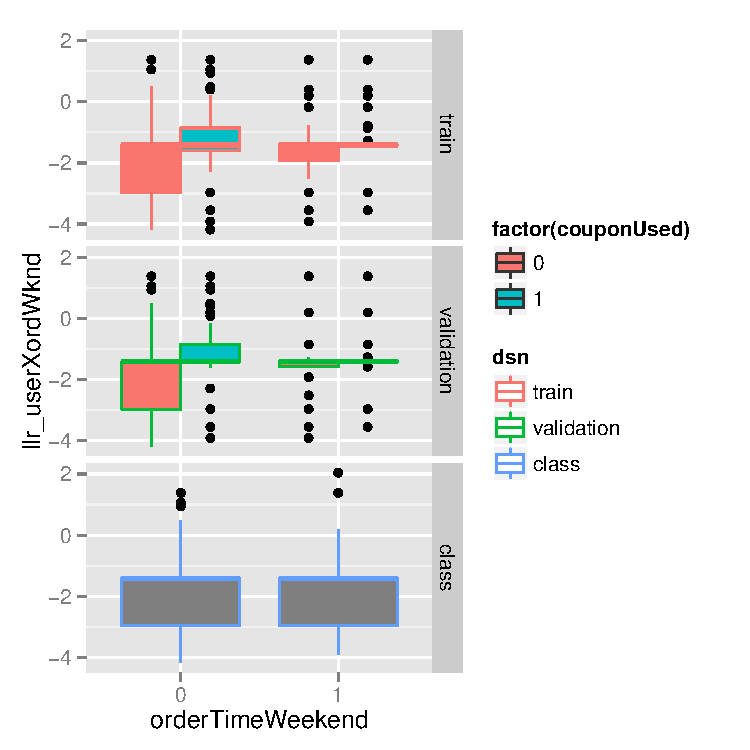
\includegraphics{/Users/user/dmc2015/ian/graphics/fig_unnamed-chunk-17-3} \end{center}

\emph{reward} (as \texttt{llr\_userXrwrd})

\begin{Shaded}
\begin{Highlighting}[]
\CommentTok{# reward}
\NormalTok{llr =}\StringTok{ }\KeywordTok{compute_ll_2w}\NormalTok{(}\KeywordTok{as.character}\NormalTok{(H$userID), }\KeywordTok{as.character}\NormalTok{(H$reward), H$couponUsed, }
    \KeywordTok{as.character}\NormalTok{(TVC$userID), }\KeywordTok{as.character}\NormalTok{(TVC$reward))}
\NormalTok{llr_userXrwrd =}\StringTok{ }\KeywordTok{data.frame}\NormalTok{(}\DataTypeTok{userID =} \NormalTok{TVC$userID, }\DataTypeTok{reward =} \NormalTok{TVC$reward, }\DataTypeTok{llr_userXrwrd =} \NormalTok{llr) %>%}\StringTok{ }
\StringTok{    }\KeywordTok{arrange}\NormalTok{(userID)}

\KeywordTok{ggplot}\NormalTok{(}\DataTypeTok{data =} \NormalTok{llr_userXrwrd, }\KeywordTok{aes}\NormalTok{(}\DataTypeTok{x =} \NormalTok{userID, }\DataTypeTok{y =} \NormalTok{reward, }\DataTypeTok{size =} \NormalTok{llr_userXrwrd), }
    \DataTypeTok{alpha =} \FloatTok{0.1}\NormalTok{) +}\StringTok{ }\KeywordTok{geom_point}\NormalTok{()}
\KeywordTok{qplot}\NormalTok{(userID, llr_userXrwrd, }\DataTypeTok{data =} \NormalTok{llr_userXrwrd, }\DataTypeTok{geom =} \StringTok{"line"}\NormalTok{, }\DataTypeTok{group =} \NormalTok{reward, }
    \DataTypeTok{facets =} \NormalTok{reward ~}\StringTok{ }\NormalTok{.)}

\NormalTok{TVC %>%}\StringTok{ }\KeywordTok{left_join}\NormalTok{(llr_userXrwrd, }\DataTypeTok{by =} \KeywordTok{c}\NormalTok{(}\StringTok{"userID"}\NormalTok{, }\StringTok{"reward"}\NormalTok{)) %>%}\StringTok{ }\KeywordTok{select}\NormalTok{(orderID, }
    \NormalTok{userID, dsn, reward, llr_userXrwrd, couponUsed) %>%}\StringTok{ }\KeywordTok{ggplot}\NormalTok{(}\KeywordTok{aes}\NormalTok{(}\DataTypeTok{x =} \NormalTok{reward, }
    \DataTypeTok{y =} \NormalTok{llr_userXrwrd, }\DataTypeTok{fill =} \KeywordTok{factor}\NormalTok{(couponUsed), }\DataTypeTok{color =} \NormalTok{dsn)) +}\StringTok{ }\KeywordTok{geom_boxplot}\NormalTok{() +}\StringTok{ }
\StringTok{    }\KeywordTok{facet_grid}\NormalTok{(dsn ~}\StringTok{ }\NormalTok{.)}
\end{Highlighting}
\end{Shaded}

\begin{verbatim}
## Warning in
## left_join_impl(x,
## y, by$x, by$y):
## joining factor and
## character vector,
## coercing into
## character vector
\end{verbatim}

\begin{verbatim}
## Warning in
## left_join_impl(x,
## y, by$x, by$y):
## joining factor and
## character vector,
## coercing into
## character vector
\end{verbatim}

\begin{Shaded}
\begin{Highlighting}[]
\NormalTok{llr_userXrwrd =}\StringTok{ }\NormalTok{TVC %>%}\StringTok{ }\KeywordTok{left_join}\NormalTok{(llr_userXrwrd, }\DataTypeTok{by =} \KeywordTok{c}\NormalTok{(}\StringTok{"userID"}\NormalTok{, }\StringTok{"reward"}\NormalTok{)) %>%}\StringTok{ }
\StringTok{    }\KeywordTok{select}\NormalTok{(orderID, dsn, llr_userXrwrd)}
\end{Highlighting}
\end{Shaded}

\begin{verbatim}
## Warning in
## left_join_impl(x,
## y, by$x, by$y):
## joining factor and
## character vector,
## coercing into
## character vector
\end{verbatim}

\begin{verbatim}
## Warning in
## left_join_impl(x,
## y, by$x, by$y):
## joining factor and
## character vector,
## coercing into
## character vector
\end{verbatim}

\begin{Shaded}
\begin{Highlighting}[]
\NormalTok{trn =}\StringTok{ }\NormalTok{llr_userXrwrd %>%}\StringTok{ }\KeywordTok{filter}\NormalTok{(dsn ==}\StringTok{ "train"}\NormalTok{) %>%}\StringTok{ }\KeywordTok{select}\NormalTok{(-dsn)}
\NormalTok{val =}\StringTok{ }\NormalTok{llr_userXrwrd %>%}\StringTok{ }\KeywordTok{filter}\NormalTok{(dsn ==}\StringTok{ "validation"}\NormalTok{) %>%}\StringTok{ }\KeywordTok{select}\NormalTok{(-dsn)}
\NormalTok{cls =}\StringTok{ }\NormalTok{llr_userXrwrd %>%}\StringTok{ }\KeywordTok{filter}\NormalTok{(dsn ==}\StringTok{ "class"}\NormalTok{) %>%}\StringTok{ }\KeywordTok{select}\NormalTok{(-dsn)}

\NormalTok{llr_userXrwrd =}\StringTok{ }\KeywordTok{list}\NormalTok{(}\DataTypeTok{T =} \NormalTok{trn, }\DataTypeTok{V =} \NormalTok{val, }\DataTypeTok{C =} \NormalTok{cls)}

\KeywordTok{saveRDS}\NormalTok{(llr_userXrwrd, }\StringTok{"../features/feature_files/llr_userXrwrd.rds"}\NormalTok{)}
\end{Highlighting}
\end{Shaded}

\begin{center}\includegraphics{/Users/user/dmc2015/ian/graphics/fig_unnamed-chunk-18-1} \includegraphics{/Users/user/dmc2015/ian/graphics/fig_unnamed-chunk-18-2} \includegraphics{/Users/user/dmc2015/ian/graphics/fig_unnamed-chunk-18-3} \end{center}

\emph{premiumProduct} (as \texttt{llr\_userXluxury})

\begin{Shaded}
\begin{Highlighting}[]
\CommentTok{# premiumProduct}
\NormalTok{llr =}\StringTok{ }\KeywordTok{compute_ll_2w}\NormalTok{(}\KeywordTok{as.character}\NormalTok{(H$userID), }\KeywordTok{as.character}\NormalTok{(H$premiumProduct), }
    \NormalTok{H$couponUsed, }\KeywordTok{as.character}\NormalTok{(TVC$userID), }\KeywordTok{as.character}\NormalTok{(TVC$premiumProduct))}
\NormalTok{llr_userXluxury =}\StringTok{ }\KeywordTok{data.frame}\NormalTok{(}\DataTypeTok{userID =} \NormalTok{TVC$userID, }\DataTypeTok{premiumProduct =} \NormalTok{TVC$premiumProduct, }
    \DataTypeTok{llr_userXluxury =} \NormalTok{llr) %>%}\StringTok{ }\KeywordTok{arrange}\NormalTok{(userID)}

\KeywordTok{ggplot}\NormalTok{(}\DataTypeTok{data =} \NormalTok{llr_userXluxury, }\KeywordTok{aes}\NormalTok{(}\DataTypeTok{x =} \NormalTok{userID, }\DataTypeTok{y =} \NormalTok{premiumProduct, }
    \DataTypeTok{size =} \NormalTok{llr_userXluxury), }\DataTypeTok{alpha =} \FloatTok{0.1}\NormalTok{) +}\StringTok{ }\KeywordTok{geom_point}\NormalTok{()}
\KeywordTok{qplot}\NormalTok{(userID, llr_userXluxury, }\DataTypeTok{data =} \NormalTok{llr_userXluxury, }\DataTypeTok{geom =} \StringTok{"line"}\NormalTok{, }
    \DataTypeTok{group =} \NormalTok{premiumProduct, }\DataTypeTok{facets =} \NormalTok{premiumProduct ~}\StringTok{ }\NormalTok{.)}

\NormalTok{TVC %>%}\StringTok{ }\KeywordTok{left_join}\NormalTok{(llr_userXluxury, }\DataTypeTok{by =} \KeywordTok{c}\NormalTok{(}\StringTok{"userID"}\NormalTok{, }\StringTok{"premiumProduct"}\NormalTok{)) %>%}\StringTok{ }
\StringTok{    }\KeywordTok{select}\NormalTok{(orderID, userID, dsn, premiumProduct, llr_userXluxury, }
        \NormalTok{couponUsed) %>%}\StringTok{ }\KeywordTok{ggplot}\NormalTok{(}\KeywordTok{aes}\NormalTok{(}\DataTypeTok{x =} \NormalTok{premiumProduct, }\DataTypeTok{y =} \NormalTok{llr_userXluxury, }
    \DataTypeTok{fill =} \KeywordTok{factor}\NormalTok{(couponUsed), }\DataTypeTok{color =} \NormalTok{dsn)) +}\StringTok{ }\KeywordTok{geom_boxplot}\NormalTok{() +}\StringTok{ }
\StringTok{    }\KeywordTok{facet_grid}\NormalTok{(dsn ~}\StringTok{ }\NormalTok{.)}
\end{Highlighting}
\end{Shaded}

\begin{verbatim}
## Warning in left_join_impl(x, y, by$x, by$y): joining factor and character
## vector, coercing into character vector
\end{verbatim}

\begin{verbatim}
## Warning in left_join_impl(x, y, by$x, by$y): joining factor and character
## vector, coercing into character vector
\end{verbatim}

\begin{Shaded}
\begin{Highlighting}[]
\NormalTok{llr_userXluxury =}\StringTok{ }\NormalTok{TVC %>%}\StringTok{ }\KeywordTok{left_join}\NormalTok{(llr_userXluxury, }\DataTypeTok{by =} \KeywordTok{c}\NormalTok{(}\StringTok{"userID"}\NormalTok{, }
    \StringTok{"premiumProduct"}\NormalTok{)) %>%}\StringTok{ }\KeywordTok{select}\NormalTok{(orderID, dsn, llr_userXluxury)}
\end{Highlighting}
\end{Shaded}

\begin{verbatim}
## Warning in left_join_impl(x, y, by$x, by$y): joining factor and character
## vector, coercing into character vector
\end{verbatim}

\begin{verbatim}
## Warning in left_join_impl(x, y, by$x, by$y): joining factor and character
## vector, coercing into character vector
\end{verbatim}

\begin{Shaded}
\begin{Highlighting}[]
\NormalTok{trn =}\StringTok{ }\NormalTok{llr_userXluxury %>%}\StringTok{ }\KeywordTok{filter}\NormalTok{(dsn ==}\StringTok{ "train"}\NormalTok{) %>%}\StringTok{ }\KeywordTok{select}\NormalTok{(-dsn)}
\NormalTok{val =}\StringTok{ }\NormalTok{llr_userXluxury %>%}\StringTok{ }\KeywordTok{filter}\NormalTok{(dsn ==}\StringTok{ "validation"}\NormalTok{) %>%}\StringTok{ }\KeywordTok{select}\NormalTok{(-dsn)}
\NormalTok{cls =}\StringTok{ }\NormalTok{llr_userXluxury %>%}\StringTok{ }\KeywordTok{filter}\NormalTok{(dsn ==}\StringTok{ "class"}\NormalTok{) %>%}\StringTok{ }\KeywordTok{select}\NormalTok{(-dsn)}

\NormalTok{llr_userXluxury =}\StringTok{ }\KeywordTok{list}\NormalTok{(}\DataTypeTok{T =} \NormalTok{trn, }\DataTypeTok{V =} \NormalTok{val, }\DataTypeTok{C =} \NormalTok{cls)}

\KeywordTok{saveRDS}\NormalTok{(llr_userXluxury, }\StringTok{"../features/feature_files/llr_userXluxury.rds"}\NormalTok{)}
\end{Highlighting}
\end{Shaded}

\begin{center}\includegraphics{/Users/user/dmc2015/ian/graphics/fig_unnamed-chunk-19-1} \includegraphics{/Users/user/dmc2015/ian/graphics/fig_unnamed-chunk-19-2} \includegraphics{/Users/user/dmc2015/ian/graphics/fig_unnamed-chunk-19-3} \end{center}

\emph{brand} (as \texttt{llr\_userXbrnd})

\begin{Shaded}
\begin{Highlighting}[]
\CommentTok{# brand}
\NormalTok{llr =}\StringTok{ }\KeywordTok{compute_ll_2w}\NormalTok{(}\KeywordTok{as.character}\NormalTok{(H$userID), }\KeywordTok{as.character}\NormalTok{(H$brand), H$couponUsed, }
    \KeywordTok{as.character}\NormalTok{(TVC$userID), }\KeywordTok{as.character}\NormalTok{(TVC$brand))}
\NormalTok{llr_userXbrnd =}\StringTok{ }\KeywordTok{data.frame}\NormalTok{(}\DataTypeTok{userID =} \NormalTok{TVC$userID, }\DataTypeTok{brand =} \NormalTok{TVC$brand, }\DataTypeTok{llr_userXbrnd =} \NormalTok{llr) %>%}\StringTok{ }
\StringTok{    }\KeywordTok{arrange}\NormalTok{(userID)}

\KeywordTok{ggplot}\NormalTok{(}\DataTypeTok{data =} \NormalTok{llr_userXbrnd, }\KeywordTok{aes}\NormalTok{(}\DataTypeTok{x =} \NormalTok{userID, }\DataTypeTok{y =} \NormalTok{brand, }\DataTypeTok{size =} \NormalTok{llr_userXbrnd), }\DataTypeTok{alpha =} \FloatTok{0.1}\NormalTok{) +}\StringTok{ }
\StringTok{    }\KeywordTok{geom_point}\NormalTok{()}
\KeywordTok{qplot}\NormalTok{(userID, llr_userXbrnd, }\DataTypeTok{data =} \NormalTok{llr_userXbrnd, }\DataTypeTok{geom =} \StringTok{"line"}\NormalTok{, }\DataTypeTok{group =} \NormalTok{brand, }
    \DataTypeTok{facets =} \NormalTok{brand ~}\StringTok{ }\NormalTok{.)}

\NormalTok{TVC %>%}\StringTok{ }\KeywordTok{left_join}\NormalTok{(llr_userXbrnd, }\DataTypeTok{by =} \KeywordTok{c}\NormalTok{(}\StringTok{"userID"}\NormalTok{, }\StringTok{"brand"}\NormalTok{)) %>%}\StringTok{ }\KeywordTok{select}\NormalTok{(orderID, userID, }
    \NormalTok{dsn, brand, llr_userXbrnd, couponUsed) %>%}\StringTok{ }\KeywordTok{ggplot}\NormalTok{(}\KeywordTok{aes}\NormalTok{(}\DataTypeTok{x =} \NormalTok{brand, }\DataTypeTok{y =} \NormalTok{llr_userXbrnd, }
    \DataTypeTok{fill =} \KeywordTok{factor}\NormalTok{(couponUsed), }\DataTypeTok{color =} \NormalTok{dsn)) +}\StringTok{ }\KeywordTok{geom_boxplot}\NormalTok{() +}\StringTok{ }\KeywordTok{facet_grid}\NormalTok{(dsn ~}\StringTok{ }
\StringTok{    }\NormalTok{.)}
\end{Highlighting}
\end{Shaded}

\begin{verbatim}
## Warning in left_join_impl(x, y, by$x, by$y): joining factor and character vector, coercing into character vector
\end{verbatim}

\begin{verbatim}
## Warning in left_join_impl(x, y, by$x, by$y): joining factor and character vector, coercing into character vector
\end{verbatim}

\begin{Shaded}
\begin{Highlighting}[]
\NormalTok{llr_userXbrnd =}\StringTok{ }\NormalTok{TVC %>%}\StringTok{ }\KeywordTok{left_join}\NormalTok{(llr_userXbrnd, }\DataTypeTok{by =} \KeywordTok{c}\NormalTok{(}\StringTok{"userID"}\NormalTok{, }\StringTok{"brand"}\NormalTok{)) %>%}\StringTok{ }\KeywordTok{select}\NormalTok{(orderID, }
    \NormalTok{dsn, llr_userXbrnd)}
\end{Highlighting}
\end{Shaded}

\begin{verbatim}
## Warning in left_join_impl(x, y, by$x, by$y): joining factor and character vector, coercing into character vector
\end{verbatim}

\begin{verbatim}
## Warning in left_join_impl(x, y, by$x, by$y): joining factor and character vector, coercing into character vector
\end{verbatim}

\begin{Shaded}
\begin{Highlighting}[]
\NormalTok{trn =}\StringTok{ }\NormalTok{llr_userXbrnd %>%}\StringTok{ }\KeywordTok{filter}\NormalTok{(dsn ==}\StringTok{ "train"}\NormalTok{) %>%}\StringTok{ }\KeywordTok{select}\NormalTok{(-dsn)}
\NormalTok{val =}\StringTok{ }\NormalTok{llr_userXbrnd %>%}\StringTok{ }\KeywordTok{filter}\NormalTok{(dsn ==}\StringTok{ "validation"}\NormalTok{) %>%}\StringTok{ }\KeywordTok{select}\NormalTok{(-dsn)}
\NormalTok{cls =}\StringTok{ }\NormalTok{llr_userXbrnd %>%}\StringTok{ }\KeywordTok{filter}\NormalTok{(dsn ==}\StringTok{ "class"}\NormalTok{) %>%}\StringTok{ }\KeywordTok{select}\NormalTok{(-dsn)}

\NormalTok{llr_userXbrnd =}\StringTok{ }\KeywordTok{list}\NormalTok{(}\DataTypeTok{T =} \NormalTok{trn, }\DataTypeTok{V =} \NormalTok{val, }\DataTypeTok{C =} \NormalTok{cls)}

\KeywordTok{saveRDS}\NormalTok{(llr_userXbrnd, }\StringTok{"../features/feature_files/llr_userXbrnd.rds"}\NormalTok{)}
\end{Highlighting}
\end{Shaded}

\begin{center}\includegraphics{/Users/user/dmc2015/ian/graphics/fig_unnamed-chunk-20-1} \includegraphics{/Users/user/dmc2015/ian/graphics/fig_unnamed-chunk-20-2} \includegraphics{/Users/user/dmc2015/ian/graphics/fig_unnamed-chunk-20-3} \end{center}

\emph{productGroup} (as \texttt{llr\_userXprod})

\begin{Shaded}
\begin{Highlighting}[]
\CommentTok{# productGroup}
\NormalTok{llr =}\StringTok{ }\KeywordTok{compute_ll_2w}\NormalTok{(}\KeywordTok{as.character}\NormalTok{(H$userID), }\KeywordTok{as.character}\NormalTok{(H$productGroup), H$couponUsed, }\KeywordTok{as.character}\NormalTok{(TVC$userID), }\KeywordTok{as.character}\NormalTok{(TVC$productGroup))}
\NormalTok{llr_userXprod =}\StringTok{ }\KeywordTok{data.frame}\NormalTok{(}\DataTypeTok{userID =} \NormalTok{TVC$userID, }\DataTypeTok{productGroup =} \NormalTok{TVC$productGroup, }\DataTypeTok{llr_userXprod =} \NormalTok{llr) %>%}\StringTok{ }\KeywordTok{arrange}\NormalTok{(userID)}

\KeywordTok{ggplot}\NormalTok{(}\DataTypeTok{data =} \NormalTok{llr_userXprod, }\KeywordTok{aes}\NormalTok{(}\DataTypeTok{x =} \NormalTok{userID, }\DataTypeTok{y =} \NormalTok{productGroup, }\DataTypeTok{size =} \NormalTok{llr_userXprod), }\DataTypeTok{alpha =} \FloatTok{0.1}\NormalTok{) +}\StringTok{ }\KeywordTok{geom_point}\NormalTok{()}
\KeywordTok{qplot}\NormalTok{(userID, llr_userXprod, }\DataTypeTok{data =} \NormalTok{llr_userXprod, }\DataTypeTok{geom =} \StringTok{"line"}\NormalTok{, }\DataTypeTok{group =} \NormalTok{productGroup, }\DataTypeTok{facets =} \NormalTok{productGroup ~}\StringTok{ }\NormalTok{.)}

\NormalTok{TVC %>%}\StringTok{ }\KeywordTok{left_join}\NormalTok{(llr_userXprod, }\DataTypeTok{by =} \KeywordTok{c}\NormalTok{(}\StringTok{"userID"}\NormalTok{, }\StringTok{"productGroup"}\NormalTok{)) %>%}\StringTok{ }\KeywordTok{select}\NormalTok{(orderID, userID, dsn, productGroup, llr_userXprod, couponUsed) %>%}\StringTok{ }\KeywordTok{ggplot}\NormalTok{(}\KeywordTok{aes}\NormalTok{(}\DataTypeTok{x =} \NormalTok{productGroup, }\DataTypeTok{y =} \NormalTok{llr_userXprod, }
    \DataTypeTok{fill =} \KeywordTok{factor}\NormalTok{(couponUsed), }\DataTypeTok{color =} \NormalTok{dsn)) +}\StringTok{ }\KeywordTok{geom_boxplot}\NormalTok{() +}\StringTok{ }\KeywordTok{facet_grid}\NormalTok{(dsn ~}\StringTok{ }\NormalTok{.)}
\end{Highlighting}
\end{Shaded}

\begin{verbatim}
## Warning in left_join_impl(x, y, by$x, by$y): joining factor and character vector, coercing into character vector
\end{verbatim}

\begin{verbatim}
## Warning in left_join_impl(x, y, by$x, by$y): joining factor and character vector, coercing into character vector
\end{verbatim}

\begin{Shaded}
\begin{Highlighting}[]
\NormalTok{llr_userXprod =}\StringTok{ }\NormalTok{TVC %>%}\StringTok{ }\KeywordTok{left_join}\NormalTok{(llr_userXprod, }\DataTypeTok{by =} \KeywordTok{c}\NormalTok{(}\StringTok{"userID"}\NormalTok{, }\StringTok{"productGroup"}\NormalTok{)) %>%}\StringTok{ }\KeywordTok{select}\NormalTok{(orderID, dsn, llr_userXprod)}
\end{Highlighting}
\end{Shaded}

\begin{verbatim}
## Warning in left_join_impl(x, y, by$x, by$y): joining factor and character vector, coercing into character vector
\end{verbatim}

\begin{verbatim}
## Warning in left_join_impl(x, y, by$x, by$y): joining factor and character vector, coercing into character vector
\end{verbatim}

\begin{Shaded}
\begin{Highlighting}[]
\NormalTok{trn =}\StringTok{ }\NormalTok{llr_userXprod %>%}\StringTok{ }\KeywordTok{filter}\NormalTok{(dsn ==}\StringTok{ "train"}\NormalTok{) %>%}\StringTok{ }\KeywordTok{select}\NormalTok{(-dsn)}
\NormalTok{val =}\StringTok{ }\NormalTok{llr_userXprod %>%}\StringTok{ }\KeywordTok{filter}\NormalTok{(dsn ==}\StringTok{ "validation"}\NormalTok{) %>%}\StringTok{ }\KeywordTok{select}\NormalTok{(-dsn)}
\NormalTok{cls =}\StringTok{ }\NormalTok{llr_userXprod %>%}\StringTok{ }\KeywordTok{filter}\NormalTok{(dsn ==}\StringTok{ "class"}\NormalTok{) %>%}\StringTok{ }\KeywordTok{select}\NormalTok{(-dsn)}

\NormalTok{llr_userXprod =}\StringTok{ }\KeywordTok{list}\NormalTok{(}\DataTypeTok{T =} \NormalTok{trn, }\DataTypeTok{V =} \NormalTok{val, }\DataTypeTok{C =} \NormalTok{cls)}

\KeywordTok{saveRDS}\NormalTok{(llr_userXprod, }\StringTok{"../features/feature_files/llr_userXprod.rds"}\NormalTok{)}
\end{Highlighting}
\end{Shaded}

\begin{center}\includegraphics{/Users/user/dmc2015/ian/graphics/fig_unnamed-chunk-21-1} \includegraphics{/Users/user/dmc2015/ian/graphics/fig_unnamed-chunk-21-2} \includegraphics{/Users/user/dmc2015/ian/graphics/fig_unnamed-chunk-21-3} \end{center}

\emph{couponCol} (as \texttt{llr\_userXcpncol})

\begin{Shaded}
\begin{Highlighting}[]
\CommentTok{# couponCol}
\NormalTok{llr =}\StringTok{ }\KeywordTok{compute_ll_2w}\NormalTok{(}\KeywordTok{as.character}\NormalTok{(H$userID), }\KeywordTok{as.character}\NormalTok{(H$couponCol), H$couponUsed, }\KeywordTok{as.character}\NormalTok{(TVC$userID), }\KeywordTok{as.character}\NormalTok{(TVC$couponCol))}
\NormalTok{llr_userXcpncol =}\StringTok{ }\KeywordTok{data.frame}\NormalTok{(}\DataTypeTok{userID =} \NormalTok{TVC$userID, }\DataTypeTok{couponCol =} \NormalTok{TVC$couponCol, }\DataTypeTok{llr_userXcpncol =} \NormalTok{llr) %>%}\StringTok{ }\KeywordTok{arrange}\NormalTok{(userID)}

\KeywordTok{ggplot}\NormalTok{(}\DataTypeTok{data =} \NormalTok{llr_userXcpncol, }\KeywordTok{aes}\NormalTok{(}\DataTypeTok{x =} \NormalTok{userID, }\DataTypeTok{y =} \NormalTok{couponCol, }\DataTypeTok{size =} \NormalTok{llr_userXcpncol), }\DataTypeTok{alpha =} \FloatTok{0.1}\NormalTok{) +}\StringTok{ }\KeywordTok{geom_point}\NormalTok{()}
\KeywordTok{qplot}\NormalTok{(userID, llr_userXcpncol, }\DataTypeTok{data =} \NormalTok{llr_userXcpncol, }\DataTypeTok{geom =} \StringTok{"line"}\NormalTok{, }\DataTypeTok{group =} \NormalTok{couponCol, }\DataTypeTok{facets =} \NormalTok{couponCol ~}\StringTok{ }\NormalTok{.)}

\NormalTok{TVC %>%}\StringTok{ }\KeywordTok{left_join}\NormalTok{(llr_userXcpncol, }\DataTypeTok{by =} \KeywordTok{c}\NormalTok{(}\StringTok{"userID"}\NormalTok{, }\StringTok{"couponCol"}\NormalTok{)) %>%}\StringTok{ }\KeywordTok{select}\NormalTok{(orderID, userID, dsn, couponCol, llr_userXcpncol, couponUsed) %>%}\StringTok{ }\KeywordTok{ggplot}\NormalTok{(}\KeywordTok{aes}\NormalTok{(}\DataTypeTok{x =} \NormalTok{couponCol, }\DataTypeTok{y =} \NormalTok{llr_userXcpncol, }
    \DataTypeTok{fill =} \KeywordTok{factor}\NormalTok{(couponUsed), }\DataTypeTok{color =} \NormalTok{dsn)) +}\StringTok{ }\KeywordTok{geom_boxplot}\NormalTok{() +}\StringTok{ }\KeywordTok{facet_grid}\NormalTok{(dsn ~}\StringTok{ }\NormalTok{.)}
\end{Highlighting}
\end{Shaded}

\begin{verbatim}
## Warning in left_join_impl(x, y, by$x, by$y): joining factor and character vector, coercing into character vector
\end{verbatim}

\begin{verbatim}
## Warning in left_join_impl(x, y, by$x, by$y): joining factor and character vector, coercing into character vector
\end{verbatim}

\begin{Shaded}
\begin{Highlighting}[]
\NormalTok{llr_userXcpncol =}\StringTok{ }\NormalTok{TVC %>%}\StringTok{ }\KeywordTok{left_join}\NormalTok{(llr_userXcpncol, }\DataTypeTok{by =} \KeywordTok{c}\NormalTok{(}\StringTok{"userID"}\NormalTok{, }\StringTok{"couponCol"}\NormalTok{)) %>%}\StringTok{ }\KeywordTok{select}\NormalTok{(orderID, dsn, llr_userXcpncol)}
\end{Highlighting}
\end{Shaded}

\begin{verbatim}
## Warning in left_join_impl(x, y, by$x, by$y): joining factor and character vector, coercing into character vector
\end{verbatim}

\begin{verbatim}
## Warning in left_join_impl(x, y, by$x, by$y): joining factor and character vector, coercing into character vector
\end{verbatim}

\begin{Shaded}
\begin{Highlighting}[]
\NormalTok{trn =}\StringTok{ }\NormalTok{llr_userXcpncol %>%}\StringTok{ }\KeywordTok{filter}\NormalTok{(dsn ==}\StringTok{ "train"}\NormalTok{) %>%}\StringTok{ }\KeywordTok{select}\NormalTok{(-dsn)}
\NormalTok{val =}\StringTok{ }\NormalTok{llr_userXcpncol %>%}\StringTok{ }\KeywordTok{filter}\NormalTok{(dsn ==}\StringTok{ "validation"}\NormalTok{) %>%}\StringTok{ }\KeywordTok{select}\NormalTok{(-dsn)}
\NormalTok{cls =}\StringTok{ }\NormalTok{llr_userXcpncol %>%}\StringTok{ }\KeywordTok{filter}\NormalTok{(dsn ==}\StringTok{ "class"}\NormalTok{) %>%}\StringTok{ }\KeywordTok{select}\NormalTok{(-dsn)}

\NormalTok{llr_userXcpncol =}\StringTok{ }\KeywordTok{list}\NormalTok{(}\DataTypeTok{T =} \NormalTok{trn, }\DataTypeTok{V =} \NormalTok{val, }\DataTypeTok{C =} \NormalTok{cls)}

\KeywordTok{saveRDS}\NormalTok{(llr_userXcpncol, }\StringTok{"../features/feature_files/llr_userXcpncol.rds"}\NormalTok{)}
\end{Highlighting}
\end{Shaded}

\begin{center}\includegraphics{/Users/user/dmc2015/ian/graphics/fig_unnamed-chunk-22-1} \includegraphics{/Users/user/dmc2015/ian/graphics/fig_unnamed-chunk-22-2} \includegraphics{/Users/user/dmc2015/ian/graphics/fig_unnamed-chunk-22-3} \end{center}

\subsection{reward and}\label{reward-and}

\emph{couponsReceivedDoW} (as \texttt{llr\_rewardXrecDoW})

\begin{Shaded}
\begin{Highlighting}[]
\CommentTok{# couponsReceivedDoW}
\NormalTok{llr =}\StringTok{ }\KeywordTok{compute_ll_2w}\NormalTok{(}\KeywordTok{as.character}\NormalTok{(H$reward), }\KeywordTok{as.character}\NormalTok{(H$couponsReceivedDoW), H$couponUsed, }\KeywordTok{as.character}\NormalTok{(TVC$reward), }\KeywordTok{as.character}\NormalTok{(TVC$couponsReceivedDoW))}
\NormalTok{llr_rewardXrecDoW =}\StringTok{ }\KeywordTok{data.frame}\NormalTok{(}\DataTypeTok{reward =} \NormalTok{TVC$reward, }\DataTypeTok{couponsReceivedDoW =} \NormalTok{TVC$couponsReceivedDoW, }\DataTypeTok{llr_rewardXrecDoW =} \NormalTok{llr) %>%}\StringTok{ }\KeywordTok{arrange}\NormalTok{(reward)}

\KeywordTok{ggplot}\NormalTok{(}\DataTypeTok{data =} \NormalTok{llr_rewardXrecDoW, }\KeywordTok{aes}\NormalTok{(}\DataTypeTok{x =} \NormalTok{reward, }\DataTypeTok{y =} \NormalTok{couponsReceivedDoW, }\DataTypeTok{size =} \NormalTok{llr_rewardXrecDoW), }\DataTypeTok{alpha =} \FloatTok{0.1}\NormalTok{) +}\StringTok{ }\KeywordTok{geom_point}\NormalTok{()}
\KeywordTok{qplot}\NormalTok{(reward, llr_rewardXrecDoW, }\DataTypeTok{data =} \NormalTok{llr_rewardXrecDoW, }\DataTypeTok{geom =} \StringTok{"line"}\NormalTok{, }\DataTypeTok{group =} \NormalTok{couponsReceivedDoW, }\DataTypeTok{facets =} \NormalTok{couponsReceivedDoW ~}\StringTok{ }\NormalTok{.)}

\NormalTok{TVC %>%}\StringTok{ }\KeywordTok{left_join}\NormalTok{(llr_rewardXrecDoW, }\DataTypeTok{by =} \KeywordTok{c}\NormalTok{(}\StringTok{"reward"}\NormalTok{, }\StringTok{"couponsReceivedDoW"}\NormalTok{)) %>%}\StringTok{ }\KeywordTok{select}\NormalTok{(orderID, reward, dsn, couponsReceivedDoW, llr_rewardXrecDoW, couponUsed) %>%}\StringTok{ }\KeywordTok{ggplot}\NormalTok{(}\KeywordTok{aes}\NormalTok{(}\DataTypeTok{x =} \NormalTok{couponsReceivedDoW, }
    \DataTypeTok{y =} \NormalTok{llr_rewardXrecDoW, }\DataTypeTok{fill =} \KeywordTok{factor}\NormalTok{(couponUsed), }\DataTypeTok{color =} \NormalTok{dsn)) +}\StringTok{ }\KeywordTok{geom_boxplot}\NormalTok{() +}\StringTok{ }\KeywordTok{facet_grid}\NormalTok{(dsn ~}\StringTok{ }\NormalTok{.)}
\end{Highlighting}
\end{Shaded}

\begin{verbatim}
## Warning in left_join_impl(x, y, by$x, by$y): joining factor and character vector, coercing into character vector
\end{verbatim}

\begin{Shaded}
\begin{Highlighting}[]
\NormalTok{llr_rewardXrecDoW =}\StringTok{ }\NormalTok{TVC %>%}\StringTok{ }\KeywordTok{left_join}\NormalTok{(llr_rewardXrecDoW, }\DataTypeTok{by =} \KeywordTok{c}\NormalTok{(}\StringTok{"reward"}\NormalTok{, }\StringTok{"couponsReceivedDoW"}\NormalTok{)) %>%}\StringTok{ }\KeywordTok{select}\NormalTok{(orderID, dsn, llr_rewardXrecDoW)}
\end{Highlighting}
\end{Shaded}

\begin{verbatim}
## Warning in left_join_impl(x, y, by$x, by$y): joining factor and character vector, coercing into character vector
\end{verbatim}

\begin{Shaded}
\begin{Highlighting}[]
\NormalTok{trn =}\StringTok{ }\NormalTok{llr_rewardXrecDoW %>%}\StringTok{ }\KeywordTok{filter}\NormalTok{(dsn ==}\StringTok{ "train"}\NormalTok{) %>%}\StringTok{ }\KeywordTok{select}\NormalTok{(-dsn)}
\NormalTok{val =}\StringTok{ }\NormalTok{llr_rewardXrecDoW %>%}\StringTok{ }\KeywordTok{filter}\NormalTok{(dsn ==}\StringTok{ "validation"}\NormalTok{) %>%}\StringTok{ }\KeywordTok{select}\NormalTok{(-dsn)}
\NormalTok{cls =}\StringTok{ }\NormalTok{llr_rewardXrecDoW %>%}\StringTok{ }\KeywordTok{filter}\NormalTok{(dsn ==}\StringTok{ "class"}\NormalTok{) %>%}\StringTok{ }\KeywordTok{select}\NormalTok{(-dsn)}

\NormalTok{llr_rewardXrecDoW =}\StringTok{ }\KeywordTok{list}\NormalTok{(}\DataTypeTok{T =} \NormalTok{trn, }\DataTypeTok{V =} \NormalTok{val, }\DataTypeTok{C =} \NormalTok{cls)}

\KeywordTok{saveRDS}\NormalTok{(llr_rewardXrecDoW, }\StringTok{"../features/feature_files/llr_rewardXrecDoW.rds"}\NormalTok{)}
\end{Highlighting}
\end{Shaded}

\begin{center}\includegraphics{/Users/user/dmc2015/ian/graphics/fig_unnamed-chunk-23-1} \includegraphics{/Users/user/dmc2015/ian/graphics/fig_unnamed-chunk-23-2} \includegraphics{/Users/user/dmc2015/ian/graphics/fig_unnamed-chunk-23-3} \end{center}

\emph{couponsReceivedFriSat} (as \texttt{llr\_rewardXrecFS})

\begin{Shaded}
\begin{Highlighting}[]
\CommentTok{# couponsReceivedFriSat}
\NormalTok{llr =}\StringTok{ }\KeywordTok{compute_ll_2w}\NormalTok{(}\KeywordTok{as.character}\NormalTok{(H$reward), }\KeywordTok{as.character}\NormalTok{(H$couponsReceivedFriSat), H$couponUsed, }\KeywordTok{as.character}\NormalTok{(TVC$reward), }\KeywordTok{as.character}\NormalTok{(TVC$couponsReceivedFriSat))}
\NormalTok{llr_rewardXrecFS =}\StringTok{ }\KeywordTok{data.frame}\NormalTok{(}\DataTypeTok{reward =} \NormalTok{TVC$reward, }\DataTypeTok{couponsReceivedFriSat =} \NormalTok{TVC$couponsReceivedFriSat, }\DataTypeTok{llr_rewardXrecFS =} \NormalTok{llr) %>%}\StringTok{ }\KeywordTok{arrange}\NormalTok{(reward)}

\KeywordTok{ggplot}\NormalTok{(}\DataTypeTok{data =} \NormalTok{llr_rewardXrecFS, }\KeywordTok{aes}\NormalTok{(}\DataTypeTok{x =} \NormalTok{reward, }\DataTypeTok{y =} \NormalTok{couponsReceivedFriSat, }\DataTypeTok{size =} \NormalTok{llr_rewardXrecFS), }\DataTypeTok{alpha =} \FloatTok{0.1}\NormalTok{) +}\StringTok{ }\KeywordTok{geom_point}\NormalTok{()}
\KeywordTok{qplot}\NormalTok{(reward, llr_rewardXrecFS, }\DataTypeTok{data =} \NormalTok{llr_rewardXrecFS, }\DataTypeTok{geom =} \StringTok{"line"}\NormalTok{, }\DataTypeTok{group =} \NormalTok{couponsReceivedFriSat, }\DataTypeTok{facets =} \NormalTok{couponsReceivedFriSat ~}\StringTok{ }\NormalTok{.)}

\NormalTok{TVC %>%}\StringTok{ }\KeywordTok{left_join}\NormalTok{(llr_rewardXrecFS, }\DataTypeTok{by =} \KeywordTok{c}\NormalTok{(}\StringTok{"reward"}\NormalTok{, }\StringTok{"couponsReceivedFriSat"}\NormalTok{)) %>%}\StringTok{ }\KeywordTok{select}\NormalTok{(orderID, reward, dsn, couponsReceivedFriSat, llr_rewardXrecFS, couponUsed) %>%}\StringTok{ }\KeywordTok{ggplot}\NormalTok{(}\KeywordTok{aes}\NormalTok{(}\DataTypeTok{x =} \NormalTok{couponsReceivedFriSat, }
    \DataTypeTok{y =} \NormalTok{llr_rewardXrecFS, }\DataTypeTok{fill =} \KeywordTok{factor}\NormalTok{(couponUsed), }\DataTypeTok{color =} \NormalTok{dsn)) +}\StringTok{ }\KeywordTok{geom_boxplot}\NormalTok{() +}\StringTok{ }\KeywordTok{facet_grid}\NormalTok{(dsn ~}\StringTok{ }\NormalTok{.)}
\end{Highlighting}
\end{Shaded}

\begin{verbatim}
## Warning in left_join_impl(x, y, by$x, by$y): joining factor and character vector, coercing into character vector
\end{verbatim}

\begin{Shaded}
\begin{Highlighting}[]
\NormalTok{llr_rewardXrecFS =}\StringTok{ }\NormalTok{TVC %>%}\StringTok{ }\KeywordTok{left_join}\NormalTok{(llr_rewardXrecFS, }\DataTypeTok{by =} \KeywordTok{c}\NormalTok{(}\StringTok{"reward"}\NormalTok{, }\StringTok{"couponsReceivedFriSat"}\NormalTok{)) %>%}\StringTok{ }\KeywordTok{select}\NormalTok{(orderID, dsn, llr_rewardXrecFS)}
\end{Highlighting}
\end{Shaded}

\begin{verbatim}
## Warning in left_join_impl(x, y, by$x, by$y): joining factor and character vector, coercing into character vector
\end{verbatim}

\begin{Shaded}
\begin{Highlighting}[]
\NormalTok{trn =}\StringTok{ }\NormalTok{llr_rewardXrecFS %>%}\StringTok{ }\KeywordTok{filter}\NormalTok{(dsn ==}\StringTok{ "train"}\NormalTok{) %>%}\StringTok{ }\KeywordTok{select}\NormalTok{(-dsn)}
\NormalTok{val =}\StringTok{ }\NormalTok{llr_rewardXrecFS %>%}\StringTok{ }\KeywordTok{filter}\NormalTok{(dsn ==}\StringTok{ "validation"}\NormalTok{) %>%}\StringTok{ }\KeywordTok{select}\NormalTok{(-dsn)}
\NormalTok{cls =}\StringTok{ }\NormalTok{llr_rewardXrecFS %>%}\StringTok{ }\KeywordTok{filter}\NormalTok{(dsn ==}\StringTok{ "class"}\NormalTok{) %>%}\StringTok{ }\KeywordTok{select}\NormalTok{(-dsn)}

\NormalTok{llr_rewardXrecFS =}\StringTok{ }\KeywordTok{list}\NormalTok{(}\DataTypeTok{T =} \NormalTok{trn, }\DataTypeTok{V =} \NormalTok{val, }\DataTypeTok{C =} \NormalTok{cls)}

\KeywordTok{saveRDS}\NormalTok{(llr_rewardXrecFS, }\StringTok{"../features/feature_files/llr_rewardXrecFS.rds"}\NormalTok{)}
\end{Highlighting}
\end{Shaded}

\begin{center}\includegraphics{/Users/user/dmc2015/ian/graphics/fig_unnamed-chunk-24-1} \includegraphics{/Users/user/dmc2015/ian/graphics/fig_unnamed-chunk-24-2} \includegraphics{/Users/user/dmc2015/ian/graphics/fig_unnamed-chunk-24-3} \end{center}

\emph{couponsReceivedWeekend} (as \texttt{llr\_rewardXrecWknd})

\begin{Shaded}
\begin{Highlighting}[]
\CommentTok{# couponsReceivedWeekend}
\NormalTok{llr =}\StringTok{ }\KeywordTok{compute_ll_2w}\NormalTok{(}\KeywordTok{as.character}\NormalTok{(H$reward), }\KeywordTok{as.character}\NormalTok{(H$couponsReceivedWeekend), H$couponUsed, }\KeywordTok{as.character}\NormalTok{(TVC$reward), }
    \KeywordTok{as.character}\NormalTok{(TVC$couponsReceivedWeekend))}
\NormalTok{llr_rewardXrecWknd =}\StringTok{ }\KeywordTok{data.frame}\NormalTok{(}\DataTypeTok{reward =} \NormalTok{TVC$reward, }\DataTypeTok{couponsReceivedWeekend =} \NormalTok{TVC$couponsReceivedWeekend, }\DataTypeTok{llr_rewardXrecWknd =} \NormalTok{llr) %>%}\StringTok{ }
\StringTok{    }\KeywordTok{arrange}\NormalTok{(reward)}

\KeywordTok{ggplot}\NormalTok{(}\DataTypeTok{data =} \NormalTok{llr_rewardXrecWknd, }\KeywordTok{aes}\NormalTok{(}\DataTypeTok{x =} \NormalTok{reward, }\DataTypeTok{y =} \NormalTok{couponsReceivedWeekend, }\DataTypeTok{size =} \NormalTok{llr_rewardXrecWknd), }\DataTypeTok{alpha =} \FloatTok{0.1}\NormalTok{) +}\StringTok{ }
\StringTok{    }\KeywordTok{geom_point}\NormalTok{()}
\KeywordTok{qplot}\NormalTok{(reward, llr_rewardXrecWknd, }\DataTypeTok{data =} \NormalTok{llr_rewardXrecWknd, }\DataTypeTok{geom =} \StringTok{"line"}\NormalTok{, }\DataTypeTok{group =} \NormalTok{couponsReceivedWeekend, }\DataTypeTok{facets =} \NormalTok{couponsReceivedWeekend ~}\StringTok{ }
\StringTok{    }\NormalTok{.)}

\NormalTok{TVC %>%}\StringTok{ }\KeywordTok{left_join}\NormalTok{(llr_rewardXrecWknd, }\DataTypeTok{by =} \KeywordTok{c}\NormalTok{(}\StringTok{"reward"}\NormalTok{, }\StringTok{"couponsReceivedWeekend"}\NormalTok{)) %>%}\StringTok{ }\KeywordTok{select}\NormalTok{(orderID, reward, dsn, couponsReceivedWeekend, }
    \NormalTok{llr_rewardXrecWknd, couponUsed) %>%}\StringTok{ }\KeywordTok{ggplot}\NormalTok{(}\KeywordTok{aes}\NormalTok{(}\DataTypeTok{x =} \NormalTok{couponsReceivedWeekend, }\DataTypeTok{y =} \NormalTok{llr_rewardXrecWknd, }\DataTypeTok{fill =} \KeywordTok{factor}\NormalTok{(couponUsed), }
    \DataTypeTok{color =} \NormalTok{dsn)) +}\StringTok{ }\KeywordTok{geom_boxplot}\NormalTok{() +}\StringTok{ }\KeywordTok{facet_grid}\NormalTok{(dsn ~}\StringTok{ }\NormalTok{.)}
\end{Highlighting}
\end{Shaded}

\begin{verbatim}
## Warning in left_join_impl(x, y, by$x, by$y): joining factor and character vector, coercing into character vector
\end{verbatim}

\begin{Shaded}
\begin{Highlighting}[]
\NormalTok{llr_rewardXrecWknd =}\StringTok{ }\NormalTok{TVC %>%}\StringTok{ }\KeywordTok{left_join}\NormalTok{(llr_rewardXrecWknd, }\DataTypeTok{by =} \KeywordTok{c}\NormalTok{(}\StringTok{"reward"}\NormalTok{, }\StringTok{"couponsReceivedWeekend"}\NormalTok{)) %>%}\StringTok{ }\KeywordTok{select}\NormalTok{(orderID, }
    \NormalTok{dsn, llr_rewardXrecWknd)}
\end{Highlighting}
\end{Shaded}

\begin{verbatim}
## Warning in left_join_impl(x, y, by$x, by$y): joining factor and character vector, coercing into character vector
\end{verbatim}

\begin{Shaded}
\begin{Highlighting}[]
\NormalTok{trn =}\StringTok{ }\NormalTok{llr_rewardXrecWknd %>%}\StringTok{ }\KeywordTok{filter}\NormalTok{(dsn ==}\StringTok{ "train"}\NormalTok{) %>%}\StringTok{ }\KeywordTok{select}\NormalTok{(-dsn)}
\NormalTok{val =}\StringTok{ }\NormalTok{llr_rewardXrecWknd %>%}\StringTok{ }\KeywordTok{filter}\NormalTok{(dsn ==}\StringTok{ "validation"}\NormalTok{) %>%}\StringTok{ }\KeywordTok{select}\NormalTok{(-dsn)}
\NormalTok{cls =}\StringTok{ }\NormalTok{llr_rewardXrecWknd %>%}\StringTok{ }\KeywordTok{filter}\NormalTok{(dsn ==}\StringTok{ "class"}\NormalTok{) %>%}\StringTok{ }\KeywordTok{select}\NormalTok{(-dsn)}

\NormalTok{llr_rewardXrecWknd =}\StringTok{ }\KeywordTok{list}\NormalTok{(}\DataTypeTok{T =} \NormalTok{trn, }\DataTypeTok{V =} \NormalTok{val, }\DataTypeTok{C =} \NormalTok{cls)}

\KeywordTok{saveRDS}\NormalTok{(llr_rewardXrecWknd, }\StringTok{"../features/feature_files/llr_rewardXrecWknd.rds"}\NormalTok{)}
\end{Highlighting}
\end{Shaded}

\begin{center}\includegraphics{/Users/user/dmc2015/ian/graphics/fig_unnamed-chunk-25-1} \includegraphics{/Users/user/dmc2015/ian/graphics/fig_unnamed-chunk-25-2} \includegraphics{/Users/user/dmc2015/ian/graphics/fig_unnamed-chunk-25-3} \end{center}

\emph{orderTimeDoW} (as \texttt{llr\_rewardXordDoW})

\begin{Shaded}
\begin{Highlighting}[]
\CommentTok{# orderTimeDoW}
\NormalTok{llr =}\StringTok{ }\KeywordTok{compute_ll_2w}\NormalTok{(}\KeywordTok{as.character}\NormalTok{(H$reward), }\KeywordTok{as.character}\NormalTok{(H$orderTimeDoW), H$couponUsed, }\KeywordTok{as.character}\NormalTok{(TVC$reward), }\KeywordTok{as.character}\NormalTok{(TVC$orderTimeDoW))}
\NormalTok{llr_rewardXordDoW =}\StringTok{ }\KeywordTok{data.frame}\NormalTok{(}\DataTypeTok{reward =} \NormalTok{TVC$reward, }\DataTypeTok{orderTimeDoW =} \NormalTok{TVC$orderTimeDoW, }\DataTypeTok{llr_rewardXordDoW =} \NormalTok{llr) %>%}\StringTok{ }\KeywordTok{arrange}\NormalTok{(reward)}

\KeywordTok{ggplot}\NormalTok{(}\DataTypeTok{data =} \NormalTok{llr_rewardXordDoW, }\KeywordTok{aes}\NormalTok{(}\DataTypeTok{x =} \NormalTok{reward, }\DataTypeTok{y =} \NormalTok{orderTimeDoW, }\DataTypeTok{size =} \NormalTok{llr_rewardXordDoW), }\DataTypeTok{alpha =} \FloatTok{0.1}\NormalTok{) +}\StringTok{ }\KeywordTok{geom_point}\NormalTok{()}
\KeywordTok{qplot}\NormalTok{(reward, llr_rewardXordDoW, }\DataTypeTok{data =} \NormalTok{llr_rewardXordDoW, }\DataTypeTok{geom =} \StringTok{"line"}\NormalTok{, }\DataTypeTok{group =} \NormalTok{orderTimeDoW, }\DataTypeTok{facets =} \NormalTok{orderTimeDoW ~}\StringTok{ }
\StringTok{    }\NormalTok{.)}

\NormalTok{TVC %>%}\StringTok{ }\KeywordTok{left_join}\NormalTok{(llr_rewardXordDoW, }\DataTypeTok{by =} \KeywordTok{c}\NormalTok{(}\StringTok{"reward"}\NormalTok{, }\StringTok{"orderTimeDoW"}\NormalTok{)) %>%}\StringTok{ }\KeywordTok{select}\NormalTok{(orderID, reward, dsn, orderTimeDoW, llr_rewardXordDoW, }
    \NormalTok{couponUsed) %>%}\StringTok{ }\KeywordTok{ggplot}\NormalTok{(}\KeywordTok{aes}\NormalTok{(}\DataTypeTok{x =} \NormalTok{orderTimeDoW, }\DataTypeTok{y =} \NormalTok{llr_rewardXordDoW, }\DataTypeTok{fill =} \KeywordTok{factor}\NormalTok{(couponUsed), }\DataTypeTok{color =} \NormalTok{dsn)) +}\StringTok{ }\KeywordTok{geom_boxplot}\NormalTok{() +}\StringTok{ }
\StringTok{    }\KeywordTok{facet_grid}\NormalTok{(dsn ~}\StringTok{ }\NormalTok{.)}
\end{Highlighting}
\end{Shaded}

\begin{verbatim}
## Warning in left_join_impl(x, y, by$x, by$y): joining factor and character vector, coercing into character vector
\end{verbatim}

\begin{Shaded}
\begin{Highlighting}[]
\NormalTok{llr_rewardXordDoW =}\StringTok{ }\NormalTok{TVC %>%}\StringTok{ }\KeywordTok{left_join}\NormalTok{(llr_rewardXordDoW, }\DataTypeTok{by =} \KeywordTok{c}\NormalTok{(}\StringTok{"reward"}\NormalTok{, }\StringTok{"orderTimeDoW"}\NormalTok{)) %>%}\StringTok{ }\KeywordTok{select}\NormalTok{(orderID, dsn, llr_rewardXordDoW)}
\end{Highlighting}
\end{Shaded}

\begin{verbatim}
## Warning in left_join_impl(x, y, by$x, by$y): joining factor and character vector, coercing into character vector
\end{verbatim}

\begin{Shaded}
\begin{Highlighting}[]
\NormalTok{trn =}\StringTok{ }\NormalTok{llr_rewardXordDoW %>%}\StringTok{ }\KeywordTok{filter}\NormalTok{(dsn ==}\StringTok{ "train"}\NormalTok{) %>%}\StringTok{ }\KeywordTok{select}\NormalTok{(-dsn)}
\NormalTok{val =}\StringTok{ }\NormalTok{llr_rewardXordDoW %>%}\StringTok{ }\KeywordTok{filter}\NormalTok{(dsn ==}\StringTok{ "validation"}\NormalTok{) %>%}\StringTok{ }\KeywordTok{select}\NormalTok{(-dsn)}
\NormalTok{cls =}\StringTok{ }\NormalTok{llr_rewardXordDoW %>%}\StringTok{ }\KeywordTok{filter}\NormalTok{(dsn ==}\StringTok{ "class"}\NormalTok{) %>%}\StringTok{ }\KeywordTok{select}\NormalTok{(-dsn)}

\NormalTok{llr_rewardXordDoW =}\StringTok{ }\KeywordTok{list}\NormalTok{(}\DataTypeTok{T =} \NormalTok{trn, }\DataTypeTok{V =} \NormalTok{val, }\DataTypeTok{C =} \NormalTok{cls)}

\KeywordTok{saveRDS}\NormalTok{(llr_rewardXordDoW, }\StringTok{"../features/feature_files/llr_rewardXordDoW.rds"}\NormalTok{)}
\end{Highlighting}
\end{Shaded}

\begin{center}\includegraphics{/Users/user/dmc2015/ian/graphics/fig_unnamed-chunk-26-1} \includegraphics{/Users/user/dmc2015/ian/graphics/fig_unnamed-chunk-26-2} \includegraphics{/Users/user/dmc2015/ian/graphics/fig_unnamed-chunk-26-3} \end{center}

\emph{orderTimeFriSat} (as \texttt{llr\_rewardXordFS})

\begin{Shaded}
\begin{Highlighting}[]
\CommentTok{# orderTimeFriSat}
\NormalTok{llr =}\StringTok{ }\KeywordTok{compute_ll_2w}\NormalTok{(}\KeywordTok{as.character}\NormalTok{(H$reward), }\KeywordTok{as.character}\NormalTok{(H$orderTimeFriSat), H$couponUsed, }\KeywordTok{as.character}\NormalTok{(TVC$reward), }\KeywordTok{as.character}\NormalTok{(TVC$orderTimeFriSat))}
\NormalTok{llr_rewardXordFS =}\StringTok{ }\KeywordTok{data.frame}\NormalTok{(}\DataTypeTok{reward =} \NormalTok{TVC$reward, }\DataTypeTok{orderTimeFriSat =} \NormalTok{TVC$orderTimeFriSat, }\DataTypeTok{llr_rewardXordFS =} \NormalTok{llr) %>%}\StringTok{ }\KeywordTok{arrange}\NormalTok{(reward)}

\KeywordTok{ggplot}\NormalTok{(}\DataTypeTok{data =} \NormalTok{llr_rewardXordFS, }\KeywordTok{aes}\NormalTok{(}\DataTypeTok{x =} \NormalTok{reward, }\DataTypeTok{y =} \NormalTok{orderTimeFriSat, }\DataTypeTok{size =} \NormalTok{llr_rewardXordFS), }\DataTypeTok{alpha =} \FloatTok{0.1}\NormalTok{) +}\StringTok{ }\KeywordTok{geom_point}\NormalTok{()}
\KeywordTok{qplot}\NormalTok{(reward, llr_rewardXordFS, }\DataTypeTok{data =} \NormalTok{llr_rewardXordFS, }\DataTypeTok{geom =} \StringTok{"line"}\NormalTok{, }\DataTypeTok{group =} \NormalTok{orderTimeFriSat, }\DataTypeTok{facets =} \NormalTok{orderTimeFriSat ~}\StringTok{ }
\StringTok{    }\NormalTok{.)}

\NormalTok{TVC %>%}\StringTok{ }\KeywordTok{left_join}\NormalTok{(llr_rewardXordFS, }\DataTypeTok{by =} \KeywordTok{c}\NormalTok{(}\StringTok{"reward"}\NormalTok{, }\StringTok{"orderTimeFriSat"}\NormalTok{)) %>%}\StringTok{ }\KeywordTok{select}\NormalTok{(orderID, reward, dsn, orderTimeFriSat, }
    \NormalTok{llr_rewardXordFS, couponUsed) %>%}\StringTok{ }\KeywordTok{ggplot}\NormalTok{(}\KeywordTok{aes}\NormalTok{(}\DataTypeTok{x =} \NormalTok{orderTimeFriSat, }\DataTypeTok{y =} \NormalTok{llr_rewardXordFS, }\DataTypeTok{fill =} \KeywordTok{factor}\NormalTok{(couponUsed), }\DataTypeTok{color =} \NormalTok{dsn)) +}\StringTok{ }
\StringTok{    }\KeywordTok{geom_boxplot}\NormalTok{() +}\StringTok{ }\KeywordTok{facet_grid}\NormalTok{(dsn ~}\StringTok{ }\NormalTok{.)}
\end{Highlighting}
\end{Shaded}

\begin{verbatim}
## Warning in left_join_impl(x, y, by$x, by$y): joining factor and character vector, coercing into character vector
\end{verbatim}

\begin{Shaded}
\begin{Highlighting}[]
\NormalTok{llr_rewardXordFS =}\StringTok{ }\NormalTok{TVC %>%}\StringTok{ }\KeywordTok{left_join}\NormalTok{(llr_rewardXordFS, }\DataTypeTok{by =} \KeywordTok{c}\NormalTok{(}\StringTok{"reward"}\NormalTok{, }\StringTok{"orderTimeFriSat"}\NormalTok{)) %>%}\StringTok{ }\KeywordTok{select}\NormalTok{(orderID, dsn, llr_rewardXordFS)}
\end{Highlighting}
\end{Shaded}

\begin{verbatim}
## Warning in left_join_impl(x, y, by$x, by$y): joining factor and character vector, coercing into character vector
\end{verbatim}

\begin{Shaded}
\begin{Highlighting}[]
\NormalTok{trn =}\StringTok{ }\NormalTok{llr_rewardXordFS %>%}\StringTok{ }\KeywordTok{filter}\NormalTok{(dsn ==}\StringTok{ "train"}\NormalTok{) %>%}\StringTok{ }\KeywordTok{select}\NormalTok{(-dsn)}
\NormalTok{val =}\StringTok{ }\NormalTok{llr_rewardXordFS %>%}\StringTok{ }\KeywordTok{filter}\NormalTok{(dsn ==}\StringTok{ "validation"}\NormalTok{) %>%}\StringTok{ }\KeywordTok{select}\NormalTok{(-dsn)}
\NormalTok{cls =}\StringTok{ }\NormalTok{llr_rewardXordFS %>%}\StringTok{ }\KeywordTok{filter}\NormalTok{(dsn ==}\StringTok{ "class"}\NormalTok{) %>%}\StringTok{ }\KeywordTok{select}\NormalTok{(-dsn)}

\NormalTok{llr_rewardXordFS =}\StringTok{ }\KeywordTok{list}\NormalTok{(}\DataTypeTok{T =} \NormalTok{trn, }\DataTypeTok{V =} \NormalTok{val, }\DataTypeTok{C =} \NormalTok{cls)}

\KeywordTok{saveRDS}\NormalTok{(llr_rewardXordFS, }\StringTok{"../features/feature_files/llr_rewardXordFS.rds"}\NormalTok{)}
\end{Highlighting}
\end{Shaded}

\begin{center}\includegraphics{/Users/user/dmc2015/ian/graphics/fig_unnamed-chunk-27-1} \includegraphics{/Users/user/dmc2015/ian/graphics/fig_unnamed-chunk-27-2} \includegraphics{/Users/user/dmc2015/ian/graphics/fig_unnamed-chunk-27-3} \end{center}

\emph{orderTimeWeekend} (as \texttt{llr\_rewardXordWknd})

\begin{Shaded}
\begin{Highlighting}[]
\CommentTok{# orderTimeWeekend}
\NormalTok{llr =}\StringTok{ }\KeywordTok{compute_ll_2w}\NormalTok{(}\KeywordTok{as.character}\NormalTok{(H$reward), }\KeywordTok{as.character}\NormalTok{(H$orderTimeWeekend), H$couponUsed, }\KeywordTok{as.character}\NormalTok{(TVC$reward), }\KeywordTok{as.character}\NormalTok{(TVC$orderTimeWeekend))}
\NormalTok{llr_rewardXordWknd =}\StringTok{ }\KeywordTok{data.frame}\NormalTok{(}\DataTypeTok{reward =} \NormalTok{TVC$reward, }\DataTypeTok{orderTimeWeekend =} \NormalTok{TVC$orderTimeWeekend, }\DataTypeTok{llr_rewardXordWknd =} \NormalTok{llr) %>%}\StringTok{ }
\StringTok{    }\KeywordTok{arrange}\NormalTok{(reward)}

\KeywordTok{ggplot}\NormalTok{(}\DataTypeTok{data =} \NormalTok{llr_rewardXordWknd, }\KeywordTok{aes}\NormalTok{(}\DataTypeTok{x =} \NormalTok{reward, }\DataTypeTok{y =} \NormalTok{orderTimeWeekend, }\DataTypeTok{size =} \NormalTok{llr_rewardXordWknd), }\DataTypeTok{alpha =} \FloatTok{0.1}\NormalTok{) +}\StringTok{ }\KeywordTok{geom_point}\NormalTok{()}
\KeywordTok{qplot}\NormalTok{(reward, llr_rewardXordWknd, }\DataTypeTok{data =} \NormalTok{llr_rewardXordWknd, }\DataTypeTok{geom =} \StringTok{"line"}\NormalTok{, }\DataTypeTok{group =} \NormalTok{orderTimeWeekend, }\DataTypeTok{facets =} \NormalTok{orderTimeWeekend ~}\StringTok{ }
\StringTok{    }\NormalTok{.)}

\NormalTok{TVC %>%}\StringTok{ }\KeywordTok{left_join}\NormalTok{(llr_rewardXordWknd, }\DataTypeTok{by =} \KeywordTok{c}\NormalTok{(}\StringTok{"reward"}\NormalTok{, }\StringTok{"orderTimeWeekend"}\NormalTok{)) %>%}\StringTok{ }\KeywordTok{select}\NormalTok{(orderID, reward, dsn, orderTimeWeekend, }
    \NormalTok{llr_rewardXordWknd, couponUsed) %>%}\StringTok{ }\KeywordTok{ggplot}\NormalTok{(}\KeywordTok{aes}\NormalTok{(}\DataTypeTok{x =} \NormalTok{orderTimeWeekend, }\DataTypeTok{y =} \NormalTok{llr_rewardXordWknd, }\DataTypeTok{fill =} \KeywordTok{factor}\NormalTok{(couponUsed), }
    \DataTypeTok{color =} \NormalTok{dsn)) +}\StringTok{ }\KeywordTok{geom_boxplot}\NormalTok{() +}\StringTok{ }\KeywordTok{facet_grid}\NormalTok{(dsn ~}\StringTok{ }\NormalTok{.)}
\end{Highlighting}
\end{Shaded}

\begin{verbatim}
## Warning in left_join_impl(x, y, by$x, by$y): joining factor and character vector, coercing into character vector
\end{verbatim}

\begin{Shaded}
\begin{Highlighting}[]
\NormalTok{llr_rewardXordWknd =}\StringTok{ }\NormalTok{TVC %>%}\StringTok{ }\KeywordTok{left_join}\NormalTok{(llr_rewardXordWknd, }\DataTypeTok{by =} \KeywordTok{c}\NormalTok{(}\StringTok{"reward"}\NormalTok{, }\StringTok{"orderTimeWeekend"}\NormalTok{)) %>%}\StringTok{ }\KeywordTok{select}\NormalTok{(orderID, dsn, }
    \NormalTok{llr_rewardXordWknd)}
\end{Highlighting}
\end{Shaded}

\begin{verbatim}
## Warning in left_join_impl(x, y, by$x, by$y): joining factor and character vector, coercing into character vector
\end{verbatim}

\begin{Shaded}
\begin{Highlighting}[]
\NormalTok{trn =}\StringTok{ }\NormalTok{llr_rewardXordWknd %>%}\StringTok{ }\KeywordTok{filter}\NormalTok{(dsn ==}\StringTok{ "train"}\NormalTok{) %>%}\StringTok{ }\KeywordTok{select}\NormalTok{(-dsn)}
\NormalTok{val =}\StringTok{ }\NormalTok{llr_rewardXordWknd %>%}\StringTok{ }\KeywordTok{filter}\NormalTok{(dsn ==}\StringTok{ "validation"}\NormalTok{) %>%}\StringTok{ }\KeywordTok{select}\NormalTok{(-dsn)}
\NormalTok{cls =}\StringTok{ }\NormalTok{llr_rewardXordWknd %>%}\StringTok{ }\KeywordTok{filter}\NormalTok{(dsn ==}\StringTok{ "class"}\NormalTok{) %>%}\StringTok{ }\KeywordTok{select}\NormalTok{(-dsn)}

\NormalTok{llr_rewardXordWknd =}\StringTok{ }\KeywordTok{list}\NormalTok{(}\DataTypeTok{T =} \NormalTok{trn, }\DataTypeTok{V =} \NormalTok{val, }\DataTypeTok{C =} \NormalTok{cls)}

\KeywordTok{saveRDS}\NormalTok{(llr_rewardXordWknd, }\StringTok{"../features/feature_files/llr_rewardXordWknd.rds"}\NormalTok{)}
\end{Highlighting}
\end{Shaded}

\begin{center}\includegraphics{/Users/user/dmc2015/ian/graphics/fig_unnamed-chunk-28-1} \includegraphics{/Users/user/dmc2015/ian/graphics/fig_unnamed-chunk-28-2} \includegraphics{/Users/user/dmc2015/ian/graphics/fig_unnamed-chunk-28-3} \end{center}

\emph{premiumProduct} (as \texttt{llr\_rewardXluxury})

\begin{Shaded}
\begin{Highlighting}[]
\CommentTok{# premiumProduct}
\NormalTok{llr =}\StringTok{ }\KeywordTok{compute_ll_2w}\NormalTok{(}\KeywordTok{as.character}\NormalTok{(H$reward), }\KeywordTok{as.character}\NormalTok{(H$premiumProduct), H$couponUsed, }\KeywordTok{as.character}\NormalTok{(TVC$reward), }\KeywordTok{as.character}\NormalTok{(TVC$premiumProduct))}
\NormalTok{llr_rewardXluxury =}\StringTok{ }\KeywordTok{data.frame}\NormalTok{(}\DataTypeTok{reward =} \NormalTok{TVC$reward, }\DataTypeTok{premiumProduct =} \NormalTok{TVC$premiumProduct, }\DataTypeTok{llr_rewardXluxury =} \NormalTok{llr) %>%}\StringTok{ }\KeywordTok{arrange}\NormalTok{(reward)}

\KeywordTok{ggplot}\NormalTok{(}\DataTypeTok{data =} \NormalTok{llr_rewardXluxury, }\KeywordTok{aes}\NormalTok{(}\DataTypeTok{x =} \NormalTok{reward, }\DataTypeTok{y =} \NormalTok{premiumProduct, }\DataTypeTok{size =} \NormalTok{llr_rewardXluxury), }\DataTypeTok{alpha =} \FloatTok{0.1}\NormalTok{) +}\StringTok{ }\KeywordTok{geom_point}\NormalTok{()}
\KeywordTok{qplot}\NormalTok{(reward, llr_rewardXluxury, }\DataTypeTok{data =} \NormalTok{llr_rewardXluxury, }\DataTypeTok{geom =} \StringTok{"line"}\NormalTok{, }\DataTypeTok{group =} \NormalTok{premiumProduct, }\DataTypeTok{facets =} \NormalTok{premiumProduct ~}\StringTok{ }
\StringTok{    }\NormalTok{.)}

\NormalTok{TVC %>%}\StringTok{ }\KeywordTok{left_join}\NormalTok{(llr_rewardXluxury, }\DataTypeTok{by =} \KeywordTok{c}\NormalTok{(}\StringTok{"reward"}\NormalTok{, }\StringTok{"premiumProduct"}\NormalTok{)) %>%}\StringTok{ }\KeywordTok{select}\NormalTok{(orderID, reward, dsn, premiumProduct, }
    \NormalTok{llr_rewardXluxury, couponUsed) %>%}\StringTok{ }\KeywordTok{ggplot}\NormalTok{(}\KeywordTok{aes}\NormalTok{(}\DataTypeTok{x =} \NormalTok{premiumProduct, }\DataTypeTok{y =} \NormalTok{llr_rewardXluxury, }\DataTypeTok{fill =} \KeywordTok{factor}\NormalTok{(couponUsed), }
    \DataTypeTok{color =} \NormalTok{dsn)) +}\StringTok{ }\KeywordTok{geom_boxplot}\NormalTok{() +}\StringTok{ }\KeywordTok{facet_grid}\NormalTok{(dsn ~}\StringTok{ }\NormalTok{.)}
\end{Highlighting}
\end{Shaded}

\begin{verbatim}
## Warning in left_join_impl(x, y, by$x, by$y): joining factor and character vector, coercing into character vector
\end{verbatim}

\begin{verbatim}
## Warning in left_join_impl(x, y, by$x, by$y): joining factor and character vector, coercing into character vector
\end{verbatim}

\begin{Shaded}
\begin{Highlighting}[]
\NormalTok{llr_rewardXluxury =}\StringTok{ }\NormalTok{TVC %>%}\StringTok{ }\KeywordTok{left_join}\NormalTok{(llr_rewardXluxury, }\DataTypeTok{by =} \KeywordTok{c}\NormalTok{(}\StringTok{"reward"}\NormalTok{, }\StringTok{"premiumProduct"}\NormalTok{)) %>%}\StringTok{ }\KeywordTok{select}\NormalTok{(orderID, dsn, llr_rewardXluxury)}
\end{Highlighting}
\end{Shaded}

\begin{verbatim}
## Warning in left_join_impl(x, y, by$x, by$y): joining factor and character vector, coercing into character vector
\end{verbatim}

\begin{verbatim}
## Warning in left_join_impl(x, y, by$x, by$y): joining factor and character vector, coercing into character vector
\end{verbatim}

\begin{Shaded}
\begin{Highlighting}[]
\NormalTok{trn =}\StringTok{ }\NormalTok{llr_rewardXluxury %>%}\StringTok{ }\KeywordTok{filter}\NormalTok{(dsn ==}\StringTok{ "train"}\NormalTok{) %>%}\StringTok{ }\KeywordTok{select}\NormalTok{(-dsn)}
\NormalTok{val =}\StringTok{ }\NormalTok{llr_rewardXluxury %>%}\StringTok{ }\KeywordTok{filter}\NormalTok{(dsn ==}\StringTok{ "validation"}\NormalTok{) %>%}\StringTok{ }\KeywordTok{select}\NormalTok{(-dsn)}
\NormalTok{cls =}\StringTok{ }\NormalTok{llr_rewardXluxury %>%}\StringTok{ }\KeywordTok{filter}\NormalTok{(dsn ==}\StringTok{ "class"}\NormalTok{) %>%}\StringTok{ }\KeywordTok{select}\NormalTok{(-dsn)}

\NormalTok{llr_rewardXluxury =}\StringTok{ }\KeywordTok{list}\NormalTok{(}\DataTypeTok{T =} \NormalTok{trn, }\DataTypeTok{V =} \NormalTok{val, }\DataTypeTok{C =} \NormalTok{cls)}

\KeywordTok{saveRDS}\NormalTok{(llr_rewardXluxury, }\StringTok{"../features/feature_files/llr_rewardXluxury.rds"}\NormalTok{)}
\end{Highlighting}
\end{Shaded}

\begin{center}\includegraphics{/Users/user/dmc2015/ian/graphics/fig_unnamed-chunk-29-1} \includegraphics{/Users/user/dmc2015/ian/graphics/fig_unnamed-chunk-29-2} \includegraphics{/Users/user/dmc2015/ian/graphics/fig_unnamed-chunk-29-3} \end{center}

\emph{brand} (as \texttt{llr\_rewardXbrnd})

\begin{Shaded}
\begin{Highlighting}[]
\CommentTok{# brand}
\NormalTok{llr =}\StringTok{ }\KeywordTok{compute_ll_2w}\NormalTok{(}\KeywordTok{as.character}\NormalTok{(H$reward), }\KeywordTok{as.character}\NormalTok{(H$brand), H$couponUsed, }\KeywordTok{as.character}\NormalTok{(TVC$reward), }\KeywordTok{as.character}\NormalTok{(TVC$brand))}
\NormalTok{llr_rewardXbrnd =}\StringTok{ }\KeywordTok{data.frame}\NormalTok{(}\DataTypeTok{reward =} \NormalTok{TVC$reward, }\DataTypeTok{brand =} \NormalTok{TVC$brand, }\DataTypeTok{llr_rewardXbrnd =} \NormalTok{llr) %>%}\StringTok{ }\KeywordTok{arrange}\NormalTok{(reward)}

\KeywordTok{ggplot}\NormalTok{(}\DataTypeTok{data =} \NormalTok{llr_rewardXbrnd, }\KeywordTok{aes}\NormalTok{(}\DataTypeTok{x =} \NormalTok{reward, }\DataTypeTok{y =} \NormalTok{brand, }\DataTypeTok{size =} \NormalTok{llr_rewardXbrnd), }\DataTypeTok{alpha =} \FloatTok{0.1}\NormalTok{) +}\StringTok{ }\KeywordTok{geom_point}\NormalTok{()}
\KeywordTok{qplot}\NormalTok{(reward, llr_rewardXbrnd, }\DataTypeTok{data =} \NormalTok{llr_rewardXbrnd, }\DataTypeTok{geom =} \StringTok{"line"}\NormalTok{, }\DataTypeTok{group =} \NormalTok{brand, }\DataTypeTok{facets =} \NormalTok{brand ~}\StringTok{ }\NormalTok{.)}

\NormalTok{TVC %>%}\StringTok{ }\KeywordTok{left_join}\NormalTok{(llr_rewardXbrnd, }\DataTypeTok{by =} \KeywordTok{c}\NormalTok{(}\StringTok{"reward"}\NormalTok{, }\StringTok{"brand"}\NormalTok{)) %>%}\StringTok{ }\KeywordTok{select}\NormalTok{(orderID, reward, dsn, brand, llr_rewardXbrnd, couponUsed) %>%}\StringTok{ }
\StringTok{    }\KeywordTok{ggplot}\NormalTok{(}\KeywordTok{aes}\NormalTok{(}\DataTypeTok{x =} \NormalTok{brand, }\DataTypeTok{y =} \NormalTok{llr_rewardXbrnd, }\DataTypeTok{fill =} \KeywordTok{factor}\NormalTok{(couponUsed), }\DataTypeTok{color =} \NormalTok{dsn)) +}\StringTok{ }\KeywordTok{geom_boxplot}\NormalTok{() +}\StringTok{ }\KeywordTok{facet_grid}\NormalTok{(dsn ~}\StringTok{ }
\StringTok{    }\NormalTok{.)}
\end{Highlighting}
\end{Shaded}

\begin{verbatim}
## Warning in left_join_impl(x, y, by$x, by$y): joining factor and character vector, coercing into character vector
\end{verbatim}

\begin{verbatim}
## Warning in left_join_impl(x, y, by$x, by$y): joining factor and character vector, coercing into character vector
\end{verbatim}

\begin{Shaded}
\begin{Highlighting}[]
\NormalTok{llr_rewardXbrnd =}\StringTok{ }\NormalTok{TVC %>%}\StringTok{ }\KeywordTok{left_join}\NormalTok{(llr_rewardXbrnd, }\DataTypeTok{by =} \KeywordTok{c}\NormalTok{(}\StringTok{"reward"}\NormalTok{, }\StringTok{"brand"}\NormalTok{)) %>%}\StringTok{ }\KeywordTok{select}\NormalTok{(orderID, dsn, llr_rewardXbrnd)}
\end{Highlighting}
\end{Shaded}

\begin{verbatim}
## Warning in left_join_impl(x, y, by$x, by$y): joining factor and character vector, coercing into character vector
\end{verbatim}

\begin{verbatim}
## Warning in left_join_impl(x, y, by$x, by$y): joining factor and character vector, coercing into character vector
\end{verbatim}

\begin{Shaded}
\begin{Highlighting}[]
\NormalTok{trn =}\StringTok{ }\NormalTok{llr_rewardXbrnd %>%}\StringTok{ }\KeywordTok{filter}\NormalTok{(dsn ==}\StringTok{ "train"}\NormalTok{) %>%}\StringTok{ }\KeywordTok{select}\NormalTok{(-dsn)}
\NormalTok{val =}\StringTok{ }\NormalTok{llr_rewardXbrnd %>%}\StringTok{ }\KeywordTok{filter}\NormalTok{(dsn ==}\StringTok{ "validation"}\NormalTok{) %>%}\StringTok{ }\KeywordTok{select}\NormalTok{(-dsn)}
\NormalTok{cls =}\StringTok{ }\NormalTok{llr_rewardXbrnd %>%}\StringTok{ }\KeywordTok{filter}\NormalTok{(dsn ==}\StringTok{ "class"}\NormalTok{) %>%}\StringTok{ }\KeywordTok{select}\NormalTok{(-dsn)}

\NormalTok{llr_rewardXbrnd =}\StringTok{ }\KeywordTok{list}\NormalTok{(}\DataTypeTok{T =} \NormalTok{trn, }\DataTypeTok{V =} \NormalTok{val, }\DataTypeTok{C =} \NormalTok{cls)}

\KeywordTok{saveRDS}\NormalTok{(llr_rewardXbrnd, }\StringTok{"../features/feature_files/llr_rewardXbrnd.rds"}\NormalTok{)}
\end{Highlighting}
\end{Shaded}

\begin{center}\includegraphics{/Users/user/dmc2015/ian/graphics/fig_unnamed-chunk-30-1} \includegraphics{/Users/user/dmc2015/ian/graphics/fig_unnamed-chunk-30-2} \includegraphics{/Users/user/dmc2015/ian/graphics/fig_unnamed-chunk-30-3} \end{center}

\emph{productGroup} (as \texttt{llr\_rewardXprod})

\begin{Shaded}
\begin{Highlighting}[]
\CommentTok{# productGroup}
\NormalTok{llr =}\StringTok{ }\KeywordTok{compute_ll_2w}\NormalTok{(}\KeywordTok{as.character}\NormalTok{(H$reward), }\KeywordTok{as.character}\NormalTok{(H$productGroup), H$couponUsed, }\KeywordTok{as.character}\NormalTok{(TVC$reward), }\KeywordTok{as.character}\NormalTok{(TVC$productGroup))}
\NormalTok{llr_rewardXprod =}\StringTok{ }\KeywordTok{data.frame}\NormalTok{(}\DataTypeTok{reward =} \NormalTok{TVC$reward, }\DataTypeTok{productGroup =} \NormalTok{TVC$productGroup, }\DataTypeTok{llr_rewardXprod =} \NormalTok{llr) %>%}\StringTok{ }\KeywordTok{arrange}\NormalTok{(reward)}

\KeywordTok{ggplot}\NormalTok{(}\DataTypeTok{data =} \NormalTok{llr_rewardXprod, }\KeywordTok{aes}\NormalTok{(}\DataTypeTok{x =} \NormalTok{reward, }\DataTypeTok{y =} \NormalTok{productGroup, }\DataTypeTok{size =} \NormalTok{llr_rewardXprod), }\DataTypeTok{alpha =} \FloatTok{0.1}\NormalTok{) +}\StringTok{ }\KeywordTok{geom_point}\NormalTok{()}
\KeywordTok{qplot}\NormalTok{(reward, llr_rewardXprod, }\DataTypeTok{data =} \NormalTok{llr_rewardXprod, }\DataTypeTok{geom =} \StringTok{"line"}\NormalTok{, }\DataTypeTok{group =} \NormalTok{productGroup, }\DataTypeTok{facets =} \NormalTok{productGroup ~}\StringTok{ }\NormalTok{.)}

\NormalTok{TVC %>%}\StringTok{ }\KeywordTok{left_join}\NormalTok{(llr_rewardXprod, }\DataTypeTok{by =} \KeywordTok{c}\NormalTok{(}\StringTok{"reward"}\NormalTok{, }\StringTok{"productGroup"}\NormalTok{)) %>%}\StringTok{ }\KeywordTok{select}\NormalTok{(orderID, reward, dsn, productGroup, llr_rewardXprod, }
    \NormalTok{couponUsed) %>%}\StringTok{ }\KeywordTok{ggplot}\NormalTok{(}\KeywordTok{aes}\NormalTok{(}\DataTypeTok{x =} \NormalTok{productGroup, }\DataTypeTok{y =} \NormalTok{llr_rewardXprod, }\DataTypeTok{fill =} \KeywordTok{factor}\NormalTok{(couponUsed), }\DataTypeTok{color =} \NormalTok{dsn)) +}\StringTok{ }\KeywordTok{geom_boxplot}\NormalTok{() +}\StringTok{ }
\StringTok{    }\KeywordTok{facet_grid}\NormalTok{(dsn ~}\StringTok{ }\NormalTok{.)}
\end{Highlighting}
\end{Shaded}

\begin{verbatim}
## Warning in left_join_impl(x, y, by$x, by$y): joining factor and character vector, coercing into character vector
\end{verbatim}

\begin{verbatim}
## Warning in left_join_impl(x, y, by$x, by$y): joining factor and character vector, coercing into character vector
\end{verbatim}

\begin{Shaded}
\begin{Highlighting}[]
\NormalTok{llr_rewardXprod =}\StringTok{ }\NormalTok{TVC %>%}\StringTok{ }\KeywordTok{left_join}\NormalTok{(llr_rewardXprod, }\DataTypeTok{by =} \KeywordTok{c}\NormalTok{(}\StringTok{"reward"}\NormalTok{, }\StringTok{"productGroup"}\NormalTok{)) %>%}\StringTok{ }\KeywordTok{select}\NormalTok{(orderID, dsn, llr_rewardXprod)}
\end{Highlighting}
\end{Shaded}

\begin{verbatim}
## Warning in left_join_impl(x, y, by$x, by$y): joining factor and character vector, coercing into character vector
\end{verbatim}

\begin{verbatim}
## Warning in left_join_impl(x, y, by$x, by$y): joining factor and character vector, coercing into character vector
\end{verbatim}

\begin{Shaded}
\begin{Highlighting}[]
\NormalTok{trn =}\StringTok{ }\NormalTok{llr_rewardXprod %>%}\StringTok{ }\KeywordTok{filter}\NormalTok{(dsn ==}\StringTok{ "train"}\NormalTok{) %>%}\StringTok{ }\KeywordTok{select}\NormalTok{(-dsn)}
\NormalTok{val =}\StringTok{ }\NormalTok{llr_rewardXprod %>%}\StringTok{ }\KeywordTok{filter}\NormalTok{(dsn ==}\StringTok{ "validation"}\NormalTok{) %>%}\StringTok{ }\KeywordTok{select}\NormalTok{(-dsn)}
\NormalTok{cls =}\StringTok{ }\NormalTok{llr_rewardXprod %>%}\StringTok{ }\KeywordTok{filter}\NormalTok{(dsn ==}\StringTok{ "class"}\NormalTok{) %>%}\StringTok{ }\KeywordTok{select}\NormalTok{(-dsn)}

\NormalTok{llr_rewardXprod =}\StringTok{ }\KeywordTok{list}\NormalTok{(}\DataTypeTok{T =} \NormalTok{trn, }\DataTypeTok{V =} \NormalTok{val, }\DataTypeTok{C =} \NormalTok{cls)}

\KeywordTok{saveRDS}\NormalTok{(llr_rewardXprod, }\StringTok{"../features/feature_files/llr_rewardXprod.rds"}\NormalTok{)}
\end{Highlighting}
\end{Shaded}

\begin{center}\includegraphics{/Users/user/dmc2015/ian/graphics/fig_unnamed-chunk-31-1} \includegraphics{/Users/user/dmc2015/ian/graphics/fig_unnamed-chunk-31-2} \includegraphics{/Users/user/dmc2015/ian/graphics/fig_unnamed-chunk-31-3} \end{center}

\emph{couponCol} (as \texttt{llr\_rewardXcpncol})

\begin{Shaded}
\begin{Highlighting}[]
\CommentTok{# couponCol}
\NormalTok{llr =}\StringTok{ }\KeywordTok{compute_ll_2w}\NormalTok{(}\KeywordTok{as.character}\NormalTok{(H$reward), }\KeywordTok{as.character}\NormalTok{(H$couponCol), H$couponUsed, }\KeywordTok{as.character}\NormalTok{(TVC$reward), }\KeywordTok{as.character}\NormalTok{(TVC$couponCol))}
\NormalTok{llr_rewardXcpncol =}\StringTok{ }\KeywordTok{data.frame}\NormalTok{(}\DataTypeTok{reward =} \NormalTok{TVC$reward, }\DataTypeTok{couponCol =} \NormalTok{TVC$couponCol, }\DataTypeTok{llr_rewardXcpncol =} \NormalTok{llr) %>%}\StringTok{ }\KeywordTok{arrange}\NormalTok{(reward)}

\KeywordTok{ggplot}\NormalTok{(}\DataTypeTok{data =} \NormalTok{llr_rewardXcpncol, }\KeywordTok{aes}\NormalTok{(}\DataTypeTok{x =} \NormalTok{reward, }\DataTypeTok{y =} \NormalTok{couponCol, }\DataTypeTok{size =} \NormalTok{llr_rewardXcpncol), }\DataTypeTok{alpha =} \FloatTok{0.1}\NormalTok{) +}\StringTok{ }\KeywordTok{geom_point}\NormalTok{()}
\KeywordTok{qplot}\NormalTok{(reward, llr_rewardXcpncol, }\DataTypeTok{data =} \NormalTok{llr_rewardXcpncol, }\DataTypeTok{geom =} \StringTok{"line"}\NormalTok{, }\DataTypeTok{group =} \NormalTok{couponCol, }\DataTypeTok{facets =} \NormalTok{couponCol ~}\StringTok{ }\NormalTok{.)}

\NormalTok{TVC %>%}\StringTok{ }\KeywordTok{left_join}\NormalTok{(llr_rewardXcpncol, }\DataTypeTok{by =} \KeywordTok{c}\NormalTok{(}\StringTok{"reward"}\NormalTok{, }\StringTok{"couponCol"}\NormalTok{)) %>%}\StringTok{ }\KeywordTok{select}\NormalTok{(orderID, reward, dsn, couponCol, llr_rewardXcpncol, }
    \NormalTok{couponUsed) %>%}\StringTok{ }\KeywordTok{ggplot}\NormalTok{(}\KeywordTok{aes}\NormalTok{(}\DataTypeTok{x =} \NormalTok{couponCol, }\DataTypeTok{y =} \NormalTok{llr_rewardXcpncol, }\DataTypeTok{fill =} \KeywordTok{factor}\NormalTok{(couponUsed), }\DataTypeTok{color =} \NormalTok{dsn)) +}\StringTok{ }\KeywordTok{geom_boxplot}\NormalTok{() +}\StringTok{ }
\StringTok{    }\KeywordTok{facet_grid}\NormalTok{(dsn ~}\StringTok{ }\NormalTok{.)}
\end{Highlighting}
\end{Shaded}

\begin{verbatim}
## Warning in left_join_impl(x, y, by$x, by$y): joining factor and character vector, coercing into character vector
\end{verbatim}

\begin{verbatim}
## Warning in left_join_impl(x, y, by$x, by$y): joining factor and character vector, coercing into character vector
\end{verbatim}

\begin{Shaded}
\begin{Highlighting}[]
\NormalTok{llr_rewardXcpncol =}\StringTok{ }\NormalTok{TVC %>%}\StringTok{ }\KeywordTok{left_join}\NormalTok{(llr_rewardXcpncol, }\DataTypeTok{by =} \KeywordTok{c}\NormalTok{(}\StringTok{"reward"}\NormalTok{, }\StringTok{"couponCol"}\NormalTok{)) %>%}\StringTok{ }\KeywordTok{select}\NormalTok{(orderID, dsn, llr_rewardXcpncol)}
\end{Highlighting}
\end{Shaded}

\begin{verbatim}
## Warning in left_join_impl(x, y, by$x, by$y): joining factor and character vector, coercing into character vector
\end{verbatim}

\begin{verbatim}
## Warning in left_join_impl(x, y, by$x, by$y): joining factor and character vector, coercing into character vector
\end{verbatim}

\begin{Shaded}
\begin{Highlighting}[]
\NormalTok{trn =}\StringTok{ }\NormalTok{llr_rewardXcpncol %>%}\StringTok{ }\KeywordTok{filter}\NormalTok{(dsn ==}\StringTok{ "train"}\NormalTok{) %>%}\StringTok{ }\KeywordTok{select}\NormalTok{(-dsn)}
\NormalTok{val =}\StringTok{ }\NormalTok{llr_rewardXcpncol %>%}\StringTok{ }\KeywordTok{filter}\NormalTok{(dsn ==}\StringTok{ "validation"}\NormalTok{) %>%}\StringTok{ }\KeywordTok{select}\NormalTok{(-dsn)}
\NormalTok{cls =}\StringTok{ }\NormalTok{llr_rewardXcpncol %>%}\StringTok{ }\KeywordTok{filter}\NormalTok{(dsn ==}\StringTok{ "class"}\NormalTok{) %>%}\StringTok{ }\KeywordTok{select}\NormalTok{(-dsn)}

\NormalTok{llr_rewardXcpncol =}\StringTok{ }\KeywordTok{list}\NormalTok{(}\DataTypeTok{T =} \NormalTok{trn, }\DataTypeTok{V =} \NormalTok{val, }\DataTypeTok{C =} \NormalTok{cls)}

\KeywordTok{saveRDS}\NormalTok{(llr_rewardXcpncol, }\StringTok{"../features/feature_files/llr_rewardXcpncol.rds"}\NormalTok{)}
\end{Highlighting}
\end{Shaded}

\begin{center}\includegraphics{/Users/user/dmc2015/ian/graphics/fig_unnamed-chunk-32-1} \includegraphics{/Users/user/dmc2015/ian/graphics/fig_unnamed-chunk-32-2} \includegraphics{/Users/user/dmc2015/ian/graphics/fig_unnamed-chunk-32-3} \end{center}

\subsection{premiumProduct and}\label{premiumproduct-and}

\emph{couponsReceivedDoW} (as \texttt{llr\_luxuryXrecDoW})

\begin{Shaded}
\begin{Highlighting}[]
\CommentTok{# couponsReceivedDoW}
\NormalTok{llr =}\StringTok{ }\KeywordTok{compute_ll_2w}\NormalTok{(}\KeywordTok{as.character}\NormalTok{(H$premiumProduct), }\KeywordTok{as.character}\NormalTok{(H$couponsReceivedDoW), H$couponUsed, }\KeywordTok{as.character}\NormalTok{(TVC$premiumProduct), }
    \KeywordTok{as.character}\NormalTok{(TVC$couponsReceivedDoW))}
\NormalTok{llr_luxuryXrecDoW =}\StringTok{ }\KeywordTok{data.frame}\NormalTok{(}\DataTypeTok{premiumProduct =} \NormalTok{TVC$premiumProduct, }\DataTypeTok{couponsReceivedDoW =} \NormalTok{TVC$couponsReceivedDoW, }\DataTypeTok{llr_luxuryXrecDoW =} \NormalTok{llr) %>%}\StringTok{ }
\StringTok{    }\KeywordTok{arrange}\NormalTok{(premiumProduct)}

\KeywordTok{ggplot}\NormalTok{(}\DataTypeTok{data =} \NormalTok{llr_luxuryXrecDoW, }\KeywordTok{aes}\NormalTok{(}\DataTypeTok{x =} \NormalTok{premiumProduct, }\DataTypeTok{y =} \NormalTok{couponsReceivedDoW, }\DataTypeTok{size =} \NormalTok{llr_luxuryXrecDoW), }\DataTypeTok{alpha =} \FloatTok{0.1}\NormalTok{) +}\StringTok{ }
\StringTok{    }\KeywordTok{geom_point}\NormalTok{()}
\KeywordTok{qplot}\NormalTok{(premiumProduct, llr_luxuryXrecDoW, }\DataTypeTok{data =} \NormalTok{llr_luxuryXrecDoW, }\DataTypeTok{geom =} \StringTok{"line"}\NormalTok{, }\DataTypeTok{group =} \NormalTok{couponsReceivedDoW, }\DataTypeTok{facets =} \NormalTok{couponsReceivedDoW ~}\StringTok{ }
\StringTok{    }\NormalTok{.)}

\NormalTok{TVC %>%}\StringTok{ }\KeywordTok{left_join}\NormalTok{(llr_luxuryXrecDoW, }\DataTypeTok{by =} \KeywordTok{c}\NormalTok{(}\StringTok{"premiumProduct"}\NormalTok{, }\StringTok{"couponsReceivedDoW"}\NormalTok{)) %>%}\StringTok{ }\KeywordTok{select}\NormalTok{(orderID, premiumProduct, }
    \NormalTok{dsn, couponsReceivedDoW, llr_luxuryXrecDoW, couponUsed) %>%}\StringTok{ }\KeywordTok{ggplot}\NormalTok{(}\KeywordTok{aes}\NormalTok{(}\DataTypeTok{x =} \NormalTok{couponsReceivedDoW, }\DataTypeTok{y =} \NormalTok{llr_luxuryXrecDoW, }
    \DataTypeTok{fill =} \KeywordTok{factor}\NormalTok{(couponUsed), }\DataTypeTok{color =} \NormalTok{dsn)) +}\StringTok{ }\KeywordTok{geom_boxplot}\NormalTok{() +}\StringTok{ }\KeywordTok{facet_grid}\NormalTok{(dsn ~}\StringTok{ }\NormalTok{.)}
\end{Highlighting}
\end{Shaded}

\begin{verbatim}
## Warning in left_join_impl(x, y, by$x, by$y): joining factor and character vector, coercing into character vector
\end{verbatim}

\begin{Shaded}
\begin{Highlighting}[]
\NormalTok{llr_luxuryXrecDoW =}\StringTok{ }\NormalTok{TVC %>%}\StringTok{ }\KeywordTok{left_join}\NormalTok{(llr_luxuryXrecDoW, }\DataTypeTok{by =} \KeywordTok{c}\NormalTok{(}\StringTok{"premiumProduct"}\NormalTok{, }\StringTok{"couponsReceivedDoW"}\NormalTok{)) %>%}\StringTok{ }\KeywordTok{select}\NormalTok{(orderID, }
    \NormalTok{dsn, llr_luxuryXrecDoW)}
\end{Highlighting}
\end{Shaded}

\begin{verbatim}
## Warning in left_join_impl(x, y, by$x, by$y): joining factor and character vector, coercing into character vector
\end{verbatim}

\begin{Shaded}
\begin{Highlighting}[]
\NormalTok{trn =}\StringTok{ }\NormalTok{llr_luxuryXrecDoW %>%}\StringTok{ }\KeywordTok{filter}\NormalTok{(dsn ==}\StringTok{ "train"}\NormalTok{) %>%}\StringTok{ }\KeywordTok{select}\NormalTok{(-dsn)}
\NormalTok{val =}\StringTok{ }\NormalTok{llr_luxuryXrecDoW %>%}\StringTok{ }\KeywordTok{filter}\NormalTok{(dsn ==}\StringTok{ "validation"}\NormalTok{) %>%}\StringTok{ }\KeywordTok{select}\NormalTok{(-dsn)}
\NormalTok{cls =}\StringTok{ }\NormalTok{llr_luxuryXrecDoW %>%}\StringTok{ }\KeywordTok{filter}\NormalTok{(dsn ==}\StringTok{ "class"}\NormalTok{) %>%}\StringTok{ }\KeywordTok{select}\NormalTok{(-dsn)}

\NormalTok{llr_luxuryXrecDoW =}\StringTok{ }\KeywordTok{list}\NormalTok{(}\DataTypeTok{T =} \NormalTok{trn, }\DataTypeTok{V =} \NormalTok{val, }\DataTypeTok{C =} \NormalTok{cls)}

\KeywordTok{saveRDS}\NormalTok{(llr_luxuryXrecDoW, }\StringTok{"../features/feature_files/llr_luxuryXrecDoW.rds"}\NormalTok{)}
\end{Highlighting}
\end{Shaded}

\begin{center}\includegraphics{/Users/user/dmc2015/ian/graphics/fig_unnamed-chunk-33-1} \includegraphics{/Users/user/dmc2015/ian/graphics/fig_unnamed-chunk-33-2} \includegraphics{/Users/user/dmc2015/ian/graphics/fig_unnamed-chunk-33-3} \end{center}

\emph{couponsReceivedFriSat} (as \texttt{llr\_luxuryXrecFS})

\begin{Shaded}
\begin{Highlighting}[]
\CommentTok{# couponsReceivedFriSat}
\NormalTok{llr =}\StringTok{ }\KeywordTok{compute_ll_2w}\NormalTok{(}\KeywordTok{as.character}\NormalTok{(H$premiumProduct), }\KeywordTok{as.character}\NormalTok{(H$couponsReceivedFriSat), H$couponUsed, }\KeywordTok{as.character}\NormalTok{(TVC$premiumProduct), }
    \KeywordTok{as.character}\NormalTok{(TVC$couponsReceivedFriSat))}
\NormalTok{llr_luxuryXrecFS =}\StringTok{ }\KeywordTok{data.frame}\NormalTok{(}\DataTypeTok{premiumProduct =} \NormalTok{TVC$premiumProduct, }\DataTypeTok{couponsReceivedFriSat =} \NormalTok{TVC$couponsReceivedFriSat, }\DataTypeTok{llr_luxuryXrecFS =} \NormalTok{llr) %>%}\StringTok{ }
\StringTok{    }\KeywordTok{arrange}\NormalTok{(premiumProduct)}

\KeywordTok{ggplot}\NormalTok{(}\DataTypeTok{data =} \NormalTok{llr_luxuryXrecFS, }\KeywordTok{aes}\NormalTok{(}\DataTypeTok{x =} \NormalTok{premiumProduct, }\DataTypeTok{y =} \NormalTok{couponsReceivedFriSat, }\DataTypeTok{size =} \NormalTok{llr_luxuryXrecFS), }\DataTypeTok{alpha =} \FloatTok{0.1}\NormalTok{) +}\StringTok{ }
\StringTok{    }\KeywordTok{geom_point}\NormalTok{()}
\KeywordTok{qplot}\NormalTok{(premiumProduct, llr_luxuryXrecFS, }\DataTypeTok{data =} \NormalTok{llr_luxuryXrecFS, }\DataTypeTok{geom =} \StringTok{"line"}\NormalTok{, }\DataTypeTok{group =} \NormalTok{couponsReceivedFriSat, }\DataTypeTok{facets =} \NormalTok{couponsReceivedFriSat ~}\StringTok{ }
\StringTok{    }\NormalTok{.)}

\NormalTok{TVC %>%}\StringTok{ }\KeywordTok{left_join}\NormalTok{(llr_luxuryXrecFS, }\DataTypeTok{by =} \KeywordTok{c}\NormalTok{(}\StringTok{"premiumProduct"}\NormalTok{, }\StringTok{"couponsReceivedFriSat"}\NormalTok{)) %>%}\StringTok{ }\KeywordTok{select}\NormalTok{(orderID, premiumProduct, }
    \NormalTok{dsn, couponsReceivedFriSat, llr_luxuryXrecFS, couponUsed) %>%}\StringTok{ }\KeywordTok{ggplot}\NormalTok{(}\KeywordTok{aes}\NormalTok{(}\DataTypeTok{x =} \NormalTok{couponsReceivedFriSat, }\DataTypeTok{y =} \NormalTok{llr_luxuryXrecFS, }
    \DataTypeTok{fill =} \KeywordTok{factor}\NormalTok{(couponUsed), }\DataTypeTok{color =} \NormalTok{dsn)) +}\StringTok{ }\KeywordTok{geom_boxplot}\NormalTok{() +}\StringTok{ }\KeywordTok{facet_grid}\NormalTok{(dsn ~}\StringTok{ }\NormalTok{.)}
\end{Highlighting}
\end{Shaded}

\begin{verbatim}
## Warning in left_join_impl(x, y, by$x, by$y): joining factor and character vector, coercing into character vector
\end{verbatim}

\begin{Shaded}
\begin{Highlighting}[]
\NormalTok{llr_luxuryXrecFS =}\StringTok{ }\NormalTok{TVC %>%}\StringTok{ }\KeywordTok{left_join}\NormalTok{(llr_luxuryXrecFS, }\DataTypeTok{by =} \KeywordTok{c}\NormalTok{(}\StringTok{"premiumProduct"}\NormalTok{, }\StringTok{"couponsReceivedFriSat"}\NormalTok{)) %>%}\StringTok{ }\KeywordTok{select}\NormalTok{(orderID, }
    \NormalTok{dsn, llr_luxuryXrecFS)}
\end{Highlighting}
\end{Shaded}

\begin{verbatim}
## Warning in left_join_impl(x, y, by$x, by$y): joining factor and character vector, coercing into character vector
\end{verbatim}

\begin{Shaded}
\begin{Highlighting}[]
\NormalTok{trn =}\StringTok{ }\NormalTok{llr_luxuryXrecFS %>%}\StringTok{ }\KeywordTok{filter}\NormalTok{(dsn ==}\StringTok{ "train"}\NormalTok{) %>%}\StringTok{ }\KeywordTok{select}\NormalTok{(-dsn)}
\NormalTok{val =}\StringTok{ }\NormalTok{llr_luxuryXrecFS %>%}\StringTok{ }\KeywordTok{filter}\NormalTok{(dsn ==}\StringTok{ "validation"}\NormalTok{) %>%}\StringTok{ }\KeywordTok{select}\NormalTok{(-dsn)}
\NormalTok{cls =}\StringTok{ }\NormalTok{llr_luxuryXrecFS %>%}\StringTok{ }\KeywordTok{filter}\NormalTok{(dsn ==}\StringTok{ "class"}\NormalTok{) %>%}\StringTok{ }\KeywordTok{select}\NormalTok{(-dsn)}

\NormalTok{llr_luxuryXrecFS =}\StringTok{ }\KeywordTok{list}\NormalTok{(}\DataTypeTok{T =} \NormalTok{trn, }\DataTypeTok{V =} \NormalTok{val, }\DataTypeTok{C =} \NormalTok{cls)}

\KeywordTok{saveRDS}\NormalTok{(llr_luxuryXrecFS, }\StringTok{"../features/feature_files/llr_luxuryXrecFS.rds"}\NormalTok{)}
\end{Highlighting}
\end{Shaded}

\begin{center}\includegraphics{/Users/user/dmc2015/ian/graphics/fig_unnamed-chunk-34-1} \includegraphics{/Users/user/dmc2015/ian/graphics/fig_unnamed-chunk-34-2} \includegraphics{/Users/user/dmc2015/ian/graphics/fig_unnamed-chunk-34-3} \end{center}

\emph{couponsReceivedWeekend} (as \texttt{llr\_luxuryXrecWknd})

\begin{Shaded}
\begin{Highlighting}[]
\CommentTok{# couponsReceivedWeekend}
\NormalTok{llr =}\StringTok{ }\KeywordTok{compute_ll_2w}\NormalTok{(}\KeywordTok{as.character}\NormalTok{(H$premiumProduct), }\KeywordTok{as.character}\NormalTok{(H$couponsReceivedWeekend), H$couponUsed, }\KeywordTok{as.character}\NormalTok{(TVC$premiumProduct), }
    \KeywordTok{as.character}\NormalTok{(TVC$couponsReceivedWeekend))}
\NormalTok{llr_luxuryXrecWknd =}\StringTok{ }\KeywordTok{data.frame}\NormalTok{(}\DataTypeTok{premiumProduct =} \NormalTok{TVC$premiumProduct, }\DataTypeTok{couponsReceivedWeekend =} \NormalTok{TVC$couponsReceivedWeekend, }
    \DataTypeTok{llr_luxuryXrecWknd =} \NormalTok{llr) %>%}\StringTok{ }\KeywordTok{arrange}\NormalTok{(premiumProduct)}

\KeywordTok{ggplot}\NormalTok{(}\DataTypeTok{data =} \NormalTok{llr_luxuryXrecWknd, }\KeywordTok{aes}\NormalTok{(}\DataTypeTok{x =} \NormalTok{premiumProduct, }\DataTypeTok{y =} \NormalTok{couponsReceivedWeekend, }\DataTypeTok{size =} \NormalTok{llr_luxuryXrecWknd), }\DataTypeTok{alpha =} \FloatTok{0.1}\NormalTok{) +}\StringTok{ }
\StringTok{    }\KeywordTok{geom_point}\NormalTok{()}
\KeywordTok{qplot}\NormalTok{(premiumProduct, llr_luxuryXrecWknd, }\DataTypeTok{data =} \NormalTok{llr_luxuryXrecWknd, }\DataTypeTok{geom =} \StringTok{"line"}\NormalTok{, }\DataTypeTok{group =} \NormalTok{couponsReceivedWeekend, }\DataTypeTok{facets =} \NormalTok{couponsReceivedWeekend ~}\StringTok{ }
\StringTok{    }\NormalTok{.)}

\NormalTok{TVC %>%}\StringTok{ }\KeywordTok{left_join}\NormalTok{(llr_luxuryXrecWknd, }\DataTypeTok{by =} \KeywordTok{c}\NormalTok{(}\StringTok{"premiumProduct"}\NormalTok{, }\StringTok{"couponsReceivedWeekend"}\NormalTok{)) %>%}\StringTok{ }\KeywordTok{select}\NormalTok{(orderID, premiumProduct, }
    \NormalTok{dsn, couponsReceivedWeekend, llr_luxuryXrecWknd, couponUsed) %>%}\StringTok{ }\KeywordTok{ggplot}\NormalTok{(}\KeywordTok{aes}\NormalTok{(}\DataTypeTok{x =} \NormalTok{couponsReceivedWeekend, }\DataTypeTok{y =} \NormalTok{llr_luxuryXrecWknd, }
    \DataTypeTok{fill =} \KeywordTok{factor}\NormalTok{(couponUsed), }\DataTypeTok{color =} \NormalTok{dsn)) +}\StringTok{ }\KeywordTok{geom_boxplot}\NormalTok{() +}\StringTok{ }\KeywordTok{facet_grid}\NormalTok{(dsn ~}\StringTok{ }\NormalTok{.)}
\end{Highlighting}
\end{Shaded}

\begin{verbatim}
## Warning in left_join_impl(x, y, by$x, by$y): joining factor and character vector, coercing into character vector
\end{verbatim}

\begin{Shaded}
\begin{Highlighting}[]
\NormalTok{llr_luxuryXrecWknd =}\StringTok{ }\NormalTok{TVC %>%}\StringTok{ }\KeywordTok{left_join}\NormalTok{(llr_luxuryXrecWknd, }\DataTypeTok{by =} \KeywordTok{c}\NormalTok{(}\StringTok{"premiumProduct"}\NormalTok{, }\StringTok{"couponsReceivedWeekend"}\NormalTok{)) %>%}\StringTok{ }\KeywordTok{select}\NormalTok{(orderID, }
    \NormalTok{dsn, llr_luxuryXrecWknd)}
\end{Highlighting}
\end{Shaded}

\begin{verbatim}
## Warning in left_join_impl(x, y, by$x, by$y): joining factor and character vector, coercing into character vector
\end{verbatim}

\begin{Shaded}
\begin{Highlighting}[]
\NormalTok{trn =}\StringTok{ }\NormalTok{llr_luxuryXrecWknd %>%}\StringTok{ }\KeywordTok{filter}\NormalTok{(dsn ==}\StringTok{ "train"}\NormalTok{) %>%}\StringTok{ }\KeywordTok{select}\NormalTok{(-dsn)}
\NormalTok{val =}\StringTok{ }\NormalTok{llr_luxuryXrecWknd %>%}\StringTok{ }\KeywordTok{filter}\NormalTok{(dsn ==}\StringTok{ "validation"}\NormalTok{) %>%}\StringTok{ }\KeywordTok{select}\NormalTok{(-dsn)}
\NormalTok{cls =}\StringTok{ }\NormalTok{llr_luxuryXrecWknd %>%}\StringTok{ }\KeywordTok{filter}\NormalTok{(dsn ==}\StringTok{ "class"}\NormalTok{) %>%}\StringTok{ }\KeywordTok{select}\NormalTok{(-dsn)}

\NormalTok{llr_luxuryXrecWknd =}\StringTok{ }\KeywordTok{list}\NormalTok{(}\DataTypeTok{T =} \NormalTok{trn, }\DataTypeTok{V =} \NormalTok{val, }\DataTypeTok{C =} \NormalTok{cls)}

\KeywordTok{saveRDS}\NormalTok{(llr_luxuryXrecWknd, }\StringTok{"../features/feature_files/llr_luxuryXrecWknd.rds"}\NormalTok{)}
\end{Highlighting}
\end{Shaded}

\begin{center}\includegraphics{/Users/user/dmc2015/ian/graphics/fig_unnamed-chunk-35-1} \includegraphics{/Users/user/dmc2015/ian/graphics/fig_unnamed-chunk-35-2} \includegraphics{/Users/user/dmc2015/ian/graphics/fig_unnamed-chunk-35-3} \end{center}

\emph{orderTimeDoW} (as \texttt{llr\_luxuryXordDoW})

\begin{Shaded}
\begin{Highlighting}[]
\CommentTok{# orderTimeDoW}
\NormalTok{llr =}\StringTok{ }\KeywordTok{compute_ll_2w}\NormalTok{(}\KeywordTok{as.character}\NormalTok{(H$premiumProduct), }\KeywordTok{as.character}\NormalTok{(H$orderTimeDoW), H$couponUsed, }\KeywordTok{as.character}\NormalTok{(TVC$premiumProduct), }
    \KeywordTok{as.character}\NormalTok{(TVC$orderTimeDoW))}
\NormalTok{llr_luxuryXordDoW =}\StringTok{ }\KeywordTok{data.frame}\NormalTok{(}\DataTypeTok{premiumProduct =} \NormalTok{TVC$premiumProduct, }\DataTypeTok{orderTimeDoW =} \NormalTok{TVC$orderTimeDoW, }\DataTypeTok{llr_luxuryXordDoW =} \NormalTok{llr) %>%}\StringTok{ }
\StringTok{    }\KeywordTok{arrange}\NormalTok{(premiumProduct)}

\KeywordTok{ggplot}\NormalTok{(}\DataTypeTok{data =} \NormalTok{llr_luxuryXordDoW, }\KeywordTok{aes}\NormalTok{(}\DataTypeTok{x =} \NormalTok{premiumProduct, }\DataTypeTok{y =} \NormalTok{orderTimeDoW, }\DataTypeTok{size =} \NormalTok{llr_luxuryXordDoW), }\DataTypeTok{alpha =} \FloatTok{0.1}\NormalTok{) +}\StringTok{ }\KeywordTok{geom_point}\NormalTok{()}
\KeywordTok{qplot}\NormalTok{(premiumProduct, llr_luxuryXordDoW, }\DataTypeTok{data =} \NormalTok{llr_luxuryXordDoW, }\DataTypeTok{geom =} \StringTok{"line"}\NormalTok{, }\DataTypeTok{group =} \NormalTok{orderTimeDoW, }\DataTypeTok{facets =} \NormalTok{orderTimeDoW ~}\StringTok{ }
\StringTok{    }\NormalTok{.)}

\NormalTok{TVC %>%}\StringTok{ }\KeywordTok{left_join}\NormalTok{(llr_luxuryXordDoW, }\DataTypeTok{by =} \KeywordTok{c}\NormalTok{(}\StringTok{"premiumProduct"}\NormalTok{, }\StringTok{"orderTimeDoW"}\NormalTok{)) %>%}\StringTok{ }\KeywordTok{select}\NormalTok{(orderID, premiumProduct, dsn, }
    \NormalTok{orderTimeDoW, llr_luxuryXordDoW, couponUsed) %>%}\StringTok{ }\KeywordTok{ggplot}\NormalTok{(}\KeywordTok{aes}\NormalTok{(}\DataTypeTok{x =} \NormalTok{orderTimeDoW, }\DataTypeTok{y =} \NormalTok{llr_luxuryXordDoW, }\DataTypeTok{fill =} \KeywordTok{factor}\NormalTok{(couponUsed), }
    \DataTypeTok{color =} \NormalTok{dsn)) +}\StringTok{ }\KeywordTok{geom_boxplot}\NormalTok{() +}\StringTok{ }\KeywordTok{facet_grid}\NormalTok{(dsn ~}\StringTok{ }\NormalTok{.)}
\end{Highlighting}
\end{Shaded}

\begin{verbatim}
## Warning in left_join_impl(x, y, by$x, by$y): joining factor and character vector, coercing into character vector
\end{verbatim}

\begin{Shaded}
\begin{Highlighting}[]
\NormalTok{llr_luxuryXordDoW =}\StringTok{ }\NormalTok{TVC %>%}\StringTok{ }\KeywordTok{left_join}\NormalTok{(llr_luxuryXordDoW, }\DataTypeTok{by =} \KeywordTok{c}\NormalTok{(}\StringTok{"premiumProduct"}\NormalTok{, }\StringTok{"orderTimeDoW"}\NormalTok{)) %>%}\StringTok{ }\KeywordTok{select}\NormalTok{(orderID, dsn, }
    \NormalTok{llr_luxuryXordDoW)}
\end{Highlighting}
\end{Shaded}

\begin{verbatim}
## Warning in left_join_impl(x, y, by$x, by$y): joining factor and character vector, coercing into character vector
\end{verbatim}

\begin{Shaded}
\begin{Highlighting}[]
\NormalTok{trn =}\StringTok{ }\NormalTok{llr_luxuryXordDoW %>%}\StringTok{ }\KeywordTok{filter}\NormalTok{(dsn ==}\StringTok{ "train"}\NormalTok{) %>%}\StringTok{ }\KeywordTok{select}\NormalTok{(-dsn)}
\NormalTok{val =}\StringTok{ }\NormalTok{llr_luxuryXordDoW %>%}\StringTok{ }\KeywordTok{filter}\NormalTok{(dsn ==}\StringTok{ "validation"}\NormalTok{) %>%}\StringTok{ }\KeywordTok{select}\NormalTok{(-dsn)}
\NormalTok{cls =}\StringTok{ }\NormalTok{llr_luxuryXordDoW %>%}\StringTok{ }\KeywordTok{filter}\NormalTok{(dsn ==}\StringTok{ "class"}\NormalTok{) %>%}\StringTok{ }\KeywordTok{select}\NormalTok{(-dsn)}

\NormalTok{llr_luxuryXordDoW =}\StringTok{ }\KeywordTok{list}\NormalTok{(}\DataTypeTok{T =} \NormalTok{trn, }\DataTypeTok{V =} \NormalTok{val, }\DataTypeTok{C =} \NormalTok{cls)}

\KeywordTok{saveRDS}\NormalTok{(llr_luxuryXordDoW, }\StringTok{"../features/feature_files/llr_luxuryXordDoW.rds"}\NormalTok{)}
\end{Highlighting}
\end{Shaded}

\begin{center}\includegraphics{/Users/user/dmc2015/ian/graphics/fig_unnamed-chunk-36-1} \includegraphics{/Users/user/dmc2015/ian/graphics/fig_unnamed-chunk-36-2} \includegraphics{/Users/user/dmc2015/ian/graphics/fig_unnamed-chunk-36-3} \end{center}

\emph{orderTimeFriSat} (as \texttt{llr\_luxuryXordFS})

\begin{Shaded}
\begin{Highlighting}[]
\CommentTok{# orderTimeFriSat}
\NormalTok{llr =}\StringTok{ }\KeywordTok{compute_ll_2w}\NormalTok{(}\KeywordTok{as.character}\NormalTok{(H$premiumProduct), }\KeywordTok{as.character}\NormalTok{(H$orderTimeFriSat), H$couponUsed, }\KeywordTok{as.character}\NormalTok{(TVC$premiumProduct), }
    \KeywordTok{as.character}\NormalTok{(TVC$orderTimeFriSat))}
\NormalTok{llr_luxuryXordFS =}\StringTok{ }\KeywordTok{data.frame}\NormalTok{(}\DataTypeTok{premiumProduct =} \NormalTok{TVC$premiumProduct, }\DataTypeTok{orderTimeFriSat =} \NormalTok{TVC$orderTimeFriSat, }\DataTypeTok{llr_luxuryXordFS =} \NormalTok{llr) %>%}\StringTok{ }
\StringTok{    }\KeywordTok{arrange}\NormalTok{(premiumProduct)}

\KeywordTok{ggplot}\NormalTok{(}\DataTypeTok{data =} \NormalTok{llr_luxuryXordFS, }\KeywordTok{aes}\NormalTok{(}\DataTypeTok{x =} \NormalTok{premiumProduct, }\DataTypeTok{y =} \NormalTok{orderTimeFriSat, }\DataTypeTok{size =} \NormalTok{llr_luxuryXordFS), }\DataTypeTok{alpha =} \FloatTok{0.1}\NormalTok{) +}\StringTok{ }\KeywordTok{geom_point}\NormalTok{()}
\KeywordTok{qplot}\NormalTok{(premiumProduct, llr_luxuryXordFS, }\DataTypeTok{data =} \NormalTok{llr_luxuryXordFS, }\DataTypeTok{geom =} \StringTok{"line"}\NormalTok{, }\DataTypeTok{group =} \NormalTok{orderTimeFriSat, }\DataTypeTok{facets =} \NormalTok{orderTimeFriSat ~}\StringTok{ }
\StringTok{    }\NormalTok{.)}

\NormalTok{TVC %>%}\StringTok{ }\KeywordTok{left_join}\NormalTok{(llr_luxuryXordFS, }\DataTypeTok{by =} \KeywordTok{c}\NormalTok{(}\StringTok{"premiumProduct"}\NormalTok{, }\StringTok{"orderTimeFriSat"}\NormalTok{)) %>%}\StringTok{ }\KeywordTok{select}\NormalTok{(orderID, premiumProduct, dsn, }
    \NormalTok{orderTimeFriSat, llr_luxuryXordFS, couponUsed) %>%}\StringTok{ }\KeywordTok{ggplot}\NormalTok{(}\KeywordTok{aes}\NormalTok{(}\DataTypeTok{x =} \NormalTok{orderTimeFriSat, }\DataTypeTok{y =} \NormalTok{llr_luxuryXordFS, }\DataTypeTok{fill =} \KeywordTok{factor}\NormalTok{(couponUsed), }
    \DataTypeTok{color =} \NormalTok{dsn)) +}\StringTok{ }\KeywordTok{geom_boxplot}\NormalTok{() +}\StringTok{ }\KeywordTok{facet_grid}\NormalTok{(dsn ~}\StringTok{ }\NormalTok{.)}
\end{Highlighting}
\end{Shaded}

\begin{verbatim}
## Warning in left_join_impl(x, y, by$x, by$y): joining factor and character vector, coercing into character vector
\end{verbatim}

\begin{Shaded}
\begin{Highlighting}[]
\NormalTok{llr_luxuryXordFS =}\StringTok{ }\NormalTok{TVC %>%}\StringTok{ }\KeywordTok{left_join}\NormalTok{(llr_luxuryXordFS, }\DataTypeTok{by =} \KeywordTok{c}\NormalTok{(}\StringTok{"premiumProduct"}\NormalTok{, }\StringTok{"orderTimeFriSat"}\NormalTok{)) %>%}\StringTok{ }\KeywordTok{select}\NormalTok{(orderID, }
    \NormalTok{dsn, llr_luxuryXordFS)}
\end{Highlighting}
\end{Shaded}

\begin{verbatim}
## Warning in left_join_impl(x, y, by$x, by$y): joining factor and character vector, coercing into character vector
\end{verbatim}

\begin{Shaded}
\begin{Highlighting}[]
\NormalTok{trn =}\StringTok{ }\NormalTok{llr_luxuryXordFS %>%}\StringTok{ }\KeywordTok{filter}\NormalTok{(dsn ==}\StringTok{ "train"}\NormalTok{) %>%}\StringTok{ }\KeywordTok{select}\NormalTok{(-dsn)}
\NormalTok{val =}\StringTok{ }\NormalTok{llr_luxuryXordFS %>%}\StringTok{ }\KeywordTok{filter}\NormalTok{(dsn ==}\StringTok{ "validation"}\NormalTok{) %>%}\StringTok{ }\KeywordTok{select}\NormalTok{(-dsn)}
\NormalTok{cls =}\StringTok{ }\NormalTok{llr_luxuryXordFS %>%}\StringTok{ }\KeywordTok{filter}\NormalTok{(dsn ==}\StringTok{ "class"}\NormalTok{) %>%}\StringTok{ }\KeywordTok{select}\NormalTok{(-dsn)}

\NormalTok{llr_luxuryXordFS =}\StringTok{ }\KeywordTok{list}\NormalTok{(}\DataTypeTok{T =} \NormalTok{trn, }\DataTypeTok{V =} \NormalTok{val, }\DataTypeTok{C =} \NormalTok{cls)}

\KeywordTok{saveRDS}\NormalTok{(llr_luxuryXordFS, }\StringTok{"../features/feature_files/llr_luxuryXordFS.rds"}\NormalTok{)}
\end{Highlighting}
\end{Shaded}

\begin{center}\includegraphics{/Users/user/dmc2015/ian/graphics/fig_unnamed-chunk-37-1} \includegraphics{/Users/user/dmc2015/ian/graphics/fig_unnamed-chunk-37-2} \includegraphics{/Users/user/dmc2015/ian/graphics/fig_unnamed-chunk-37-3} \end{center}

\emph{orderTimeWeekend} (as \texttt{llr\_luxuryXordWknd})

\begin{Shaded}
\begin{Highlighting}[]
\CommentTok{# orderTimeWeekend}
\NormalTok{llr =}\StringTok{ }\KeywordTok{compute_ll_2w}\NormalTok{(}\KeywordTok{as.character}\NormalTok{(H$premiumProduct), }\KeywordTok{as.character}\NormalTok{(H$orderTimeWeekend), H$couponUsed, }\KeywordTok{as.character}\NormalTok{(TVC$premiumProduct), }
    \KeywordTok{as.character}\NormalTok{(TVC$orderTimeWeekend))}
\NormalTok{llr_luxuryXordWknd =}\StringTok{ }\KeywordTok{data.frame}\NormalTok{(}\DataTypeTok{premiumProduct =} \NormalTok{TVC$premiumProduct, }\DataTypeTok{orderTimeWeekend =} \NormalTok{TVC$orderTimeWeekend, }\DataTypeTok{llr_luxuryXordWknd =} \NormalTok{llr) %>%}\StringTok{ }
\StringTok{    }\KeywordTok{arrange}\NormalTok{(premiumProduct)}

\KeywordTok{ggplot}\NormalTok{(}\DataTypeTok{data =} \NormalTok{llr_luxuryXordWknd, }\KeywordTok{aes}\NormalTok{(}\DataTypeTok{x =} \NormalTok{premiumProduct, }\DataTypeTok{y =} \NormalTok{orderTimeWeekend, }\DataTypeTok{size =} \NormalTok{llr_luxuryXordWknd), }\DataTypeTok{alpha =} \FloatTok{0.1}\NormalTok{) +}\StringTok{ }
\StringTok{    }\KeywordTok{geom_point}\NormalTok{()}
\KeywordTok{qplot}\NormalTok{(premiumProduct, llr_luxuryXordWknd, }\DataTypeTok{data =} \NormalTok{llr_luxuryXordWknd, }\DataTypeTok{geom =} \StringTok{"line"}\NormalTok{, }\DataTypeTok{group =} \NormalTok{orderTimeWeekend, }\DataTypeTok{facets =} \NormalTok{orderTimeWeekend ~}\StringTok{ }
\StringTok{    }\NormalTok{.)}

\NormalTok{TVC %>%}\StringTok{ }\KeywordTok{left_join}\NormalTok{(llr_luxuryXordWknd, }\DataTypeTok{by =} \KeywordTok{c}\NormalTok{(}\StringTok{"premiumProduct"}\NormalTok{, }\StringTok{"orderTimeWeekend"}\NormalTok{)) %>%}\StringTok{ }\KeywordTok{select}\NormalTok{(orderID, premiumProduct, }
    \NormalTok{dsn, orderTimeWeekend, llr_luxuryXordWknd, couponUsed) %>%}\StringTok{ }\KeywordTok{ggplot}\NormalTok{(}\KeywordTok{aes}\NormalTok{(}\DataTypeTok{x =} \NormalTok{orderTimeWeekend, }\DataTypeTok{y =} \NormalTok{llr_luxuryXordWknd, }
    \DataTypeTok{fill =} \KeywordTok{factor}\NormalTok{(couponUsed), }\DataTypeTok{color =} \NormalTok{dsn)) +}\StringTok{ }\KeywordTok{geom_boxplot}\NormalTok{() +}\StringTok{ }\KeywordTok{facet_grid}\NormalTok{(dsn ~}\StringTok{ }\NormalTok{.)}
\end{Highlighting}
\end{Shaded}

\begin{verbatim}
## Warning in left_join_impl(x, y, by$x, by$y): joining factor and character vector, coercing into character vector
\end{verbatim}

\begin{Shaded}
\begin{Highlighting}[]
\NormalTok{llr_luxuryXordWknd =}\StringTok{ }\NormalTok{TVC %>%}\StringTok{ }\KeywordTok{left_join}\NormalTok{(llr_luxuryXordWknd, }\DataTypeTok{by =} \KeywordTok{c}\NormalTok{(}\StringTok{"premiumProduct"}\NormalTok{, }\StringTok{"orderTimeWeekend"}\NormalTok{)) %>%}\StringTok{ }\KeywordTok{select}\NormalTok{(orderID, }
    \NormalTok{dsn, llr_luxuryXordWknd)}
\end{Highlighting}
\end{Shaded}

\begin{verbatim}
## Warning in left_join_impl(x, y, by$x, by$y): joining factor and character vector, coercing into character vector
\end{verbatim}

\begin{Shaded}
\begin{Highlighting}[]
\NormalTok{trn =}\StringTok{ }\NormalTok{llr_luxuryXordWknd %>%}\StringTok{ }\KeywordTok{filter}\NormalTok{(dsn ==}\StringTok{ "train"}\NormalTok{) %>%}\StringTok{ }\KeywordTok{select}\NormalTok{(-dsn)}
\NormalTok{val =}\StringTok{ }\NormalTok{llr_luxuryXordWknd %>%}\StringTok{ }\KeywordTok{filter}\NormalTok{(dsn ==}\StringTok{ "validation"}\NormalTok{) %>%}\StringTok{ }\KeywordTok{select}\NormalTok{(-dsn)}
\NormalTok{cls =}\StringTok{ }\NormalTok{llr_luxuryXordWknd %>%}\StringTok{ }\KeywordTok{filter}\NormalTok{(dsn ==}\StringTok{ "class"}\NormalTok{) %>%}\StringTok{ }\KeywordTok{select}\NormalTok{(-dsn)}

\NormalTok{llr_luxuryXordWknd =}\StringTok{ }\KeywordTok{list}\NormalTok{(}\DataTypeTok{T =} \NormalTok{trn, }\DataTypeTok{V =} \NormalTok{val, }\DataTypeTok{C =} \NormalTok{cls)}

\KeywordTok{saveRDS}\NormalTok{(llr_luxuryXordWknd, }\StringTok{"../features/feature_files/llr_luxuryXordWknd.rds"}\NormalTok{)}
\end{Highlighting}
\end{Shaded}

\begin{center}\includegraphics{/Users/user/dmc2015/ian/graphics/fig_unnamed-chunk-38-1} \includegraphics{/Users/user/dmc2015/ian/graphics/fig_unnamed-chunk-38-2} \includegraphics{/Users/user/dmc2015/ian/graphics/fig_unnamed-chunk-38-3} \end{center}

\emph{brand} (as \texttt{llr\_luxuryXbrnd})

\begin{Shaded}
\begin{Highlighting}[]
\CommentTok{# brand}
\NormalTok{llr =}\StringTok{ }\KeywordTok{compute_ll_2w}\NormalTok{(}\KeywordTok{as.character}\NormalTok{(H$premiumProduct), }\KeywordTok{as.character}\NormalTok{(H$brand), H$couponUsed, }\KeywordTok{as.character}\NormalTok{(TVC$premiumProduct), }
    \KeywordTok{as.character}\NormalTok{(TVC$brand))}
\NormalTok{llr_luxuryXbrnd =}\StringTok{ }\KeywordTok{data.frame}\NormalTok{(}\DataTypeTok{premiumProduct =} \NormalTok{TVC$premiumProduct, }\DataTypeTok{brand =} \NormalTok{TVC$brand, }\DataTypeTok{llr_luxuryXbrnd =} \NormalTok{llr) %>%}\StringTok{ }\KeywordTok{arrange}\NormalTok{(premiumProduct)}

\KeywordTok{ggplot}\NormalTok{(}\DataTypeTok{data =} \NormalTok{llr_luxuryXbrnd, }\KeywordTok{aes}\NormalTok{(}\DataTypeTok{x =} \NormalTok{premiumProduct, }\DataTypeTok{y =} \NormalTok{brand, }\DataTypeTok{size =} \NormalTok{llr_luxuryXbrnd), }\DataTypeTok{alpha =} \FloatTok{0.1}\NormalTok{) +}\StringTok{ }\KeywordTok{geom_point}\NormalTok{()}
\KeywordTok{qplot}\NormalTok{(premiumProduct, llr_luxuryXbrnd, }\DataTypeTok{data =} \NormalTok{llr_luxuryXbrnd, }\DataTypeTok{geom =} \StringTok{"line"}\NormalTok{, }\DataTypeTok{group =} \NormalTok{brand, }\DataTypeTok{facets =} \NormalTok{brand ~}\StringTok{ }\NormalTok{.)}

\NormalTok{TVC %>%}\StringTok{ }\KeywordTok{left_join}\NormalTok{(llr_luxuryXbrnd, }\DataTypeTok{by =} \KeywordTok{c}\NormalTok{(}\StringTok{"premiumProduct"}\NormalTok{, }\StringTok{"brand"}\NormalTok{)) %>%}\StringTok{ }\KeywordTok{select}\NormalTok{(orderID, premiumProduct, dsn, brand, llr_luxuryXbrnd, }
    \NormalTok{couponUsed) %>%}\StringTok{ }\KeywordTok{ggplot}\NormalTok{(}\KeywordTok{aes}\NormalTok{(}\DataTypeTok{x =} \NormalTok{brand, }\DataTypeTok{y =} \NormalTok{llr_luxuryXbrnd, }\DataTypeTok{fill =} \KeywordTok{factor}\NormalTok{(couponUsed), }\DataTypeTok{color =} \NormalTok{dsn)) +}\StringTok{ }\KeywordTok{geom_boxplot}\NormalTok{() +}\StringTok{ }
\StringTok{    }\KeywordTok{facet_grid}\NormalTok{(dsn ~}\StringTok{ }\NormalTok{.)}
\end{Highlighting}
\end{Shaded}

\begin{verbatim}
## Warning in left_join_impl(x, y, by$x, by$y): joining factor and character vector, coercing into character vector
\end{verbatim}

\begin{verbatim}
## Warning in left_join_impl(x, y, by$x, by$y): joining factor and character vector, coercing into character vector
\end{verbatim}

\begin{Shaded}
\begin{Highlighting}[]
\NormalTok{llr_luxuryXbrnd =}\StringTok{ }\NormalTok{TVC %>%}\StringTok{ }\KeywordTok{left_join}\NormalTok{(llr_luxuryXbrnd, }\DataTypeTok{by =} \KeywordTok{c}\NormalTok{(}\StringTok{"premiumProduct"}\NormalTok{, }\StringTok{"brand"}\NormalTok{)) %>%}\StringTok{ }\KeywordTok{select}\NormalTok{(orderID, dsn, llr_luxuryXbrnd)}
\end{Highlighting}
\end{Shaded}

\begin{verbatim}
## Warning in left_join_impl(x, y, by$x, by$y): joining factor and character vector, coercing into character vector
\end{verbatim}

\begin{verbatim}
## Warning in left_join_impl(x, y, by$x, by$y): joining factor and character vector, coercing into character vector
\end{verbatim}

\begin{Shaded}
\begin{Highlighting}[]
\NormalTok{trn =}\StringTok{ }\NormalTok{llr_luxuryXbrnd %>%}\StringTok{ }\KeywordTok{filter}\NormalTok{(dsn ==}\StringTok{ "train"}\NormalTok{) %>%}\StringTok{ }\KeywordTok{select}\NormalTok{(-dsn)}
\NormalTok{val =}\StringTok{ }\NormalTok{llr_luxuryXbrnd %>%}\StringTok{ }\KeywordTok{filter}\NormalTok{(dsn ==}\StringTok{ "validation"}\NormalTok{) %>%}\StringTok{ }\KeywordTok{select}\NormalTok{(-dsn)}
\NormalTok{cls =}\StringTok{ }\NormalTok{llr_luxuryXbrnd %>%}\StringTok{ }\KeywordTok{filter}\NormalTok{(dsn ==}\StringTok{ "class"}\NormalTok{) %>%}\StringTok{ }\KeywordTok{select}\NormalTok{(-dsn)}

\NormalTok{llr_luxuryXbrnd =}\StringTok{ }\KeywordTok{list}\NormalTok{(}\DataTypeTok{T =} \NormalTok{trn, }\DataTypeTok{V =} \NormalTok{val, }\DataTypeTok{C =} \NormalTok{cls)}

\KeywordTok{saveRDS}\NormalTok{(llr_luxuryXbrnd, }\StringTok{"../features/feature_files/llr_luxuryXbrnd.rds"}\NormalTok{)}
\end{Highlighting}
\end{Shaded}

\begin{center}\includegraphics{/Users/user/dmc2015/ian/graphics/fig_unnamed-chunk-39-1} \includegraphics{/Users/user/dmc2015/ian/graphics/fig_unnamed-chunk-39-2} \includegraphics{/Users/user/dmc2015/ian/graphics/fig_unnamed-chunk-39-3} \end{center}

\emph{productGroup} (as \texttt{llr\_luxuryXprod})

\begin{Shaded}
\begin{Highlighting}[]
\CommentTok{# productGroup}
\NormalTok{llr =}\StringTok{ }\KeywordTok{compute_ll_2w}\NormalTok{(}\KeywordTok{as.character}\NormalTok{(H$premiumProduct), }\KeywordTok{as.character}\NormalTok{(H$productGroup), H$couponUsed, }\KeywordTok{as.character}\NormalTok{(TVC$premiumProduct), }
    \KeywordTok{as.character}\NormalTok{(TVC$productGroup))}
\NormalTok{llr_luxuryXprod =}\StringTok{ }\KeywordTok{data.frame}\NormalTok{(}\DataTypeTok{premiumProduct =} \NormalTok{TVC$premiumProduct, }\DataTypeTok{productGroup =} \NormalTok{TVC$productGroup, }\DataTypeTok{llr_luxuryXprod =} \NormalTok{llr) %>%}\StringTok{ }
\StringTok{    }\KeywordTok{arrange}\NormalTok{(premiumProduct)}

\KeywordTok{ggplot}\NormalTok{(}\DataTypeTok{data =} \NormalTok{llr_luxuryXprod, }\KeywordTok{aes}\NormalTok{(}\DataTypeTok{x =} \NormalTok{premiumProduct, }\DataTypeTok{y =} \NormalTok{productGroup, }\DataTypeTok{size =} \NormalTok{llr_luxuryXprod), }\DataTypeTok{alpha =} \FloatTok{0.1}\NormalTok{) +}\StringTok{ }\KeywordTok{geom_point}\NormalTok{()}
\KeywordTok{qplot}\NormalTok{(premiumProduct, llr_luxuryXprod, }\DataTypeTok{data =} \NormalTok{llr_luxuryXprod, }\DataTypeTok{geom =} \StringTok{"line"}\NormalTok{, }\DataTypeTok{group =} \NormalTok{productGroup, }\DataTypeTok{facets =} \NormalTok{productGroup ~}\StringTok{ }
\StringTok{    }\NormalTok{.)}

\NormalTok{TVC %>%}\StringTok{ }\KeywordTok{left_join}\NormalTok{(llr_luxuryXprod, }\DataTypeTok{by =} \KeywordTok{c}\NormalTok{(}\StringTok{"premiumProduct"}\NormalTok{, }\StringTok{"productGroup"}\NormalTok{)) %>%}\StringTok{ }\KeywordTok{select}\NormalTok{(orderID, premiumProduct, dsn, productGroup, }
    \NormalTok{llr_luxuryXprod, couponUsed) %>%}\StringTok{ }\KeywordTok{ggplot}\NormalTok{(}\KeywordTok{aes}\NormalTok{(}\DataTypeTok{x =} \NormalTok{productGroup, }\DataTypeTok{y =} \NormalTok{llr_luxuryXprod, }\DataTypeTok{fill =} \KeywordTok{factor}\NormalTok{(couponUsed), }\DataTypeTok{color =} \NormalTok{dsn)) +}\StringTok{ }
\StringTok{    }\KeywordTok{geom_boxplot}\NormalTok{() +}\StringTok{ }\KeywordTok{facet_grid}\NormalTok{(dsn ~}\StringTok{ }\NormalTok{.)}
\end{Highlighting}
\end{Shaded}

\begin{verbatim}
## Warning in left_join_impl(x, y, by$x, by$y): joining factor and character vector, coercing into character vector
\end{verbatim}

\begin{verbatim}
## Warning in left_join_impl(x, y, by$x, by$y): joining factor and character vector, coercing into character vector
\end{verbatim}

\begin{Shaded}
\begin{Highlighting}[]
\NormalTok{llr_luxuryXprod =}\StringTok{ }\NormalTok{TVC %>%}\StringTok{ }\KeywordTok{left_join}\NormalTok{(llr_luxuryXprod, }\DataTypeTok{by =} \KeywordTok{c}\NormalTok{(}\StringTok{"premiumProduct"}\NormalTok{, }\StringTok{"productGroup"}\NormalTok{)) %>%}\StringTok{ }\KeywordTok{select}\NormalTok{(orderID, dsn, }
    \NormalTok{llr_luxuryXprod)}
\end{Highlighting}
\end{Shaded}

\begin{verbatim}
## Warning in left_join_impl(x, y, by$x, by$y): joining factor and character vector, coercing into character vector
\end{verbatim}

\begin{verbatim}
## Warning in left_join_impl(x, y, by$x, by$y): joining factor and character vector, coercing into character vector
\end{verbatim}

\begin{Shaded}
\begin{Highlighting}[]
\NormalTok{trn =}\StringTok{ }\NormalTok{llr_luxuryXprod %>%}\StringTok{ }\KeywordTok{filter}\NormalTok{(dsn ==}\StringTok{ "train"}\NormalTok{) %>%}\StringTok{ }\KeywordTok{select}\NormalTok{(-dsn)}
\NormalTok{val =}\StringTok{ }\NormalTok{llr_luxuryXprod %>%}\StringTok{ }\KeywordTok{filter}\NormalTok{(dsn ==}\StringTok{ "validation"}\NormalTok{) %>%}\StringTok{ }\KeywordTok{select}\NormalTok{(-dsn)}
\NormalTok{cls =}\StringTok{ }\NormalTok{llr_luxuryXprod %>%}\StringTok{ }\KeywordTok{filter}\NormalTok{(dsn ==}\StringTok{ "class"}\NormalTok{) %>%}\StringTok{ }\KeywordTok{select}\NormalTok{(-dsn)}

\NormalTok{llr_luxuryXprod =}\StringTok{ }\KeywordTok{list}\NormalTok{(}\DataTypeTok{T =} \NormalTok{trn, }\DataTypeTok{V =} \NormalTok{val, }\DataTypeTok{C =} \NormalTok{cls)}

\KeywordTok{saveRDS}\NormalTok{(llr_luxuryXprod, }\StringTok{"../features/feature_files/llr_luxuryXprod.rds"}\NormalTok{)}
\end{Highlighting}
\end{Shaded}

\begin{center}\includegraphics{/Users/user/dmc2015/ian/graphics/fig_unnamed-chunk-40-1} \includegraphics{/Users/user/dmc2015/ian/graphics/fig_unnamed-chunk-40-2} \includegraphics{/Users/user/dmc2015/ian/graphics/fig_unnamed-chunk-40-3} \end{center}

\emph{couponCol} (as \texttt{llr\_luxuryXcpncol})

\begin{Shaded}
\begin{Highlighting}[]
\CommentTok{# couponCol}
\NormalTok{llr =}\StringTok{ }\KeywordTok{compute_ll_2w}\NormalTok{(}\KeywordTok{as.character}\NormalTok{(H$premiumProduct), }\KeywordTok{as.character}\NormalTok{(H$couponCol), H$couponUsed, }\KeywordTok{as.character}\NormalTok{(TVC$premiumProduct), }
    \KeywordTok{as.character}\NormalTok{(TVC$couponCol))}
\NormalTok{llr_luxuryXcpncol =}\StringTok{ }\KeywordTok{data.frame}\NormalTok{(}\DataTypeTok{premiumProduct =} \NormalTok{TVC$premiumProduct, }\DataTypeTok{couponCol =} \NormalTok{TVC$couponCol, }\DataTypeTok{llr_luxuryXcpncol =} \NormalTok{llr) %>%}\StringTok{ }
\StringTok{    }\KeywordTok{arrange}\NormalTok{(premiumProduct)}

\KeywordTok{ggplot}\NormalTok{(}\DataTypeTok{data =} \NormalTok{llr_luxuryXcpncol, }\KeywordTok{aes}\NormalTok{(}\DataTypeTok{x =} \NormalTok{premiumProduct, }\DataTypeTok{y =} \NormalTok{couponCol, }\DataTypeTok{size =} \NormalTok{llr_luxuryXcpncol), }\DataTypeTok{alpha =} \FloatTok{0.1}\NormalTok{) +}\StringTok{ }\KeywordTok{geom_point}\NormalTok{()}
\KeywordTok{qplot}\NormalTok{(premiumProduct, llr_luxuryXcpncol, }\DataTypeTok{data =} \NormalTok{llr_luxuryXcpncol, }\DataTypeTok{geom =} \StringTok{"line"}\NormalTok{, }\DataTypeTok{group =} \NormalTok{couponCol, }\DataTypeTok{facets =} \NormalTok{couponCol ~}\StringTok{ }
\StringTok{    }\NormalTok{.)}

\NormalTok{TVC %>%}\StringTok{ }\KeywordTok{left_join}\NormalTok{(llr_luxuryXcpncol, }\DataTypeTok{by =} \KeywordTok{c}\NormalTok{(}\StringTok{"premiumProduct"}\NormalTok{, }\StringTok{"couponCol"}\NormalTok{)) %>%}\StringTok{ }\KeywordTok{select}\NormalTok{(orderID, premiumProduct, dsn, couponCol, }
    \NormalTok{llr_luxuryXcpncol, couponUsed) %>%}\StringTok{ }\KeywordTok{ggplot}\NormalTok{(}\KeywordTok{aes}\NormalTok{(}\DataTypeTok{x =} \NormalTok{couponCol, }\DataTypeTok{y =} \NormalTok{llr_luxuryXcpncol, }\DataTypeTok{fill =} \KeywordTok{factor}\NormalTok{(couponUsed), }\DataTypeTok{color =} \NormalTok{dsn)) +}\StringTok{ }
\StringTok{    }\KeywordTok{geom_boxplot}\NormalTok{() +}\StringTok{ }\KeywordTok{facet_grid}\NormalTok{(dsn ~}\StringTok{ }\NormalTok{.)}
\end{Highlighting}
\end{Shaded}

\begin{verbatim}
## Warning in left_join_impl(x, y, by$x, by$y): joining factor and character vector, coercing into character vector
\end{verbatim}

\begin{verbatim}
## Warning in left_join_impl(x, y, by$x, by$y): joining factor and character vector, coercing into character vector
\end{verbatim}

\begin{Shaded}
\begin{Highlighting}[]
\NormalTok{llr_luxuryXcpncol =}\StringTok{ }\NormalTok{TVC %>%}\StringTok{ }\KeywordTok{left_join}\NormalTok{(llr_luxuryXcpncol, }\DataTypeTok{by =} \KeywordTok{c}\NormalTok{(}\StringTok{"premiumProduct"}\NormalTok{, }\StringTok{"couponCol"}\NormalTok{)) %>%}\StringTok{ }\KeywordTok{select}\NormalTok{(orderID, dsn, }
    \NormalTok{llr_luxuryXcpncol)}
\end{Highlighting}
\end{Shaded}

\begin{verbatim}
## Warning in left_join_impl(x, y, by$x, by$y): joining factor and character vector, coercing into character vector
\end{verbatim}

\begin{verbatim}
## Warning in left_join_impl(x, y, by$x, by$y): joining factor and character vector, coercing into character vector
\end{verbatim}

\begin{Shaded}
\begin{Highlighting}[]
\NormalTok{trn =}\StringTok{ }\NormalTok{llr_luxuryXcpncol %>%}\StringTok{ }\KeywordTok{filter}\NormalTok{(dsn ==}\StringTok{ "train"}\NormalTok{) %>%}\StringTok{ }\KeywordTok{select}\NormalTok{(-dsn)}
\NormalTok{val =}\StringTok{ }\NormalTok{llr_luxuryXcpncol %>%}\StringTok{ }\KeywordTok{filter}\NormalTok{(dsn ==}\StringTok{ "validation"}\NormalTok{) %>%}\StringTok{ }\KeywordTok{select}\NormalTok{(-dsn)}
\NormalTok{cls =}\StringTok{ }\NormalTok{llr_luxuryXcpncol %>%}\StringTok{ }\KeywordTok{filter}\NormalTok{(dsn ==}\StringTok{ "class"}\NormalTok{) %>%}\StringTok{ }\KeywordTok{select}\NormalTok{(-dsn)}

\NormalTok{llr_luxuryXcpncol =}\StringTok{ }\KeywordTok{list}\NormalTok{(}\DataTypeTok{T =} \NormalTok{trn, }\DataTypeTok{V =} \NormalTok{val, }\DataTypeTok{C =} \NormalTok{cls)}

\KeywordTok{saveRDS}\NormalTok{(llr_luxuryXcpncol, }\StringTok{"../features/feature_files/llr_luxuryXcpncol.rds"}\NormalTok{)}
\end{Highlighting}
\end{Shaded}

\begin{center}\includegraphics{/Users/user/dmc2015/ian/graphics/fig_unnamed-chunk-41-1} \includegraphics{/Users/user/dmc2015/ian/graphics/fig_unnamed-chunk-41-2} \includegraphics{/Users/user/dmc2015/ian/graphics/fig_unnamed-chunk-41-3} \end{center}

\subsection{brand and}\label{brand-and}

\emph{couponsReceivedDoW} (as \texttt{llr\_brandXrecDoW})

\begin{Shaded}
\begin{Highlighting}[]
\CommentTok{# couponsReceivedDoW}
\NormalTok{llr =}\StringTok{ }\KeywordTok{compute_ll_2w}\NormalTok{(}\KeywordTok{as.character}\NormalTok{(H$brand), }\KeywordTok{as.character}\NormalTok{(H$couponsReceivedDoW), H$couponUsed, }\KeywordTok{as.character}\NormalTok{(TVC$brand), }\KeywordTok{as.character}\NormalTok{(TVC$couponsReceivedDoW))}
\NormalTok{llr_brandXrecDoW =}\StringTok{ }\KeywordTok{data.frame}\NormalTok{(}\DataTypeTok{brand =} \NormalTok{TVC$brand, }\DataTypeTok{couponsReceivedDoW =} \NormalTok{TVC$couponsReceivedDoW, }\DataTypeTok{llr_brandXrecDoW =} \NormalTok{llr) %>%}\StringTok{ }
\StringTok{    }\KeywordTok{arrange}\NormalTok{(brand)}

\KeywordTok{ggplot}\NormalTok{(}\DataTypeTok{data =} \NormalTok{llr_brandXrecDoW, }\KeywordTok{aes}\NormalTok{(}\DataTypeTok{x =} \NormalTok{brand, }\DataTypeTok{y =} \NormalTok{couponsReceivedDoW, }\DataTypeTok{size =} \NormalTok{llr_brandXrecDoW), }\DataTypeTok{alpha =} \FloatTok{0.1}\NormalTok{) +}\StringTok{ }\KeywordTok{geom_point}\NormalTok{()}
\KeywordTok{qplot}\NormalTok{(brand, llr_brandXrecDoW, }\DataTypeTok{data =} \NormalTok{llr_brandXrecDoW, }\DataTypeTok{geom =} \StringTok{"line"}\NormalTok{, }\DataTypeTok{group =} \NormalTok{couponsReceivedDoW, }\DataTypeTok{facets =} \NormalTok{couponsReceivedDoW ~}\StringTok{ }
\StringTok{    }\NormalTok{.)}

\NormalTok{TVC %>%}\StringTok{ }\KeywordTok{left_join}\NormalTok{(llr_brandXrecDoW, }\DataTypeTok{by =} \KeywordTok{c}\NormalTok{(}\StringTok{"brand"}\NormalTok{, }\StringTok{"couponsReceivedDoW"}\NormalTok{)) %>%}\StringTok{ }\KeywordTok{select}\NormalTok{(orderID, brand, dsn, couponsReceivedDoW, }
    \NormalTok{llr_brandXrecDoW, couponUsed) %>%}\StringTok{ }\KeywordTok{ggplot}\NormalTok{(}\KeywordTok{aes}\NormalTok{(}\DataTypeTok{x =} \NormalTok{couponsReceivedDoW, }\DataTypeTok{y =} \NormalTok{llr_brandXrecDoW, }\DataTypeTok{fill =} \KeywordTok{factor}\NormalTok{(couponUsed), }
    \DataTypeTok{color =} \NormalTok{dsn)) +}\StringTok{ }\KeywordTok{geom_boxplot}\NormalTok{() +}\StringTok{ }\KeywordTok{facet_grid}\NormalTok{(dsn ~}\StringTok{ }\NormalTok{.)}
\end{Highlighting}
\end{Shaded}

\begin{verbatim}
## Warning in left_join_impl(x, y, by$x, by$y): joining factor and character vector, coercing into character vector
\end{verbatim}

\begin{Shaded}
\begin{Highlighting}[]
\NormalTok{llr_brandXrecDoW =}\StringTok{ }\NormalTok{TVC %>%}\StringTok{ }\KeywordTok{left_join}\NormalTok{(llr_brandXrecDoW, }\DataTypeTok{by =} \KeywordTok{c}\NormalTok{(}\StringTok{"brand"}\NormalTok{, }\StringTok{"couponsReceivedDoW"}\NormalTok{)) %>%}\StringTok{ }\KeywordTok{select}\NormalTok{(orderID, dsn, llr_brandXrecDoW)}
\end{Highlighting}
\end{Shaded}

\begin{verbatim}
## Warning in left_join_impl(x, y, by$x, by$y): joining factor and character vector, coercing into character vector
\end{verbatim}

\begin{Shaded}
\begin{Highlighting}[]
\NormalTok{trn =}\StringTok{ }\NormalTok{llr_brandXrecDoW %>%}\StringTok{ }\KeywordTok{filter}\NormalTok{(dsn ==}\StringTok{ "train"}\NormalTok{) %>%}\StringTok{ }\KeywordTok{select}\NormalTok{(-dsn)}
\NormalTok{val =}\StringTok{ }\NormalTok{llr_brandXrecDoW %>%}\StringTok{ }\KeywordTok{filter}\NormalTok{(dsn ==}\StringTok{ "validation"}\NormalTok{) %>%}\StringTok{ }\KeywordTok{select}\NormalTok{(-dsn)}
\NormalTok{cls =}\StringTok{ }\NormalTok{llr_brandXrecDoW %>%}\StringTok{ }\KeywordTok{filter}\NormalTok{(dsn ==}\StringTok{ "class"}\NormalTok{) %>%}\StringTok{ }\KeywordTok{select}\NormalTok{(-dsn)}

\NormalTok{llr_brandXrecDoW =}\StringTok{ }\KeywordTok{list}\NormalTok{(}\DataTypeTok{T =} \NormalTok{trn, }\DataTypeTok{V =} \NormalTok{val, }\DataTypeTok{C =} \NormalTok{cls)}

\KeywordTok{saveRDS}\NormalTok{(llr_brandXrecDoW, }\StringTok{"../features/feature_files/llr_brandXrecDoW.rds"}\NormalTok{)}
\end{Highlighting}
\end{Shaded}

\begin{center}\includegraphics{/Users/user/dmc2015/ian/graphics/fig_unnamed-chunk-42-1} \includegraphics{/Users/user/dmc2015/ian/graphics/fig_unnamed-chunk-42-2} \includegraphics{/Users/user/dmc2015/ian/graphics/fig_unnamed-chunk-42-3} \end{center}

\emph{couponsReceivedFriSat} (as \texttt{llr\_brandXrecFS})

\begin{Shaded}
\begin{Highlighting}[]
\CommentTok{# couponsReceivedFriSat}
\NormalTok{llr =}\StringTok{ }\KeywordTok{compute_ll_2w}\NormalTok{(}\KeywordTok{as.character}\NormalTok{(H$brand), }\KeywordTok{as.character}\NormalTok{(H$couponsReceivedFriSat), H$couponUsed, }\KeywordTok{as.character}\NormalTok{(TVC$brand), }
    \KeywordTok{as.character}\NormalTok{(TVC$couponsReceivedFriSat))}
\NormalTok{llr_brandXrecFS =}\StringTok{ }\KeywordTok{data.frame}\NormalTok{(}\DataTypeTok{brand =} \NormalTok{TVC$brand, }\DataTypeTok{couponsReceivedFriSat =} \NormalTok{TVC$couponsReceivedFriSat, }\DataTypeTok{llr_brandXrecFS =} \NormalTok{llr) %>%}\StringTok{ }
\StringTok{    }\KeywordTok{arrange}\NormalTok{(brand)}

\KeywordTok{ggplot}\NormalTok{(}\DataTypeTok{data =} \NormalTok{llr_brandXrecFS, }\KeywordTok{aes}\NormalTok{(}\DataTypeTok{x =} \NormalTok{brand, }\DataTypeTok{y =} \NormalTok{couponsReceivedFriSat, }\DataTypeTok{size =} \NormalTok{llr_brandXrecFS), }\DataTypeTok{alpha =} \FloatTok{0.1}\NormalTok{) +}\StringTok{ }\KeywordTok{geom_point}\NormalTok{()}
\KeywordTok{qplot}\NormalTok{(brand, llr_brandXrecFS, }\DataTypeTok{data =} \NormalTok{llr_brandXrecFS, }\DataTypeTok{geom =} \StringTok{"line"}\NormalTok{, }\DataTypeTok{group =} \NormalTok{couponsReceivedFriSat, }\DataTypeTok{facets =} \NormalTok{couponsReceivedFriSat ~}\StringTok{ }
\StringTok{    }\NormalTok{.)}

\NormalTok{TVC %>%}\StringTok{ }\KeywordTok{left_join}\NormalTok{(llr_brandXrecFS, }\DataTypeTok{by =} \KeywordTok{c}\NormalTok{(}\StringTok{"brand"}\NormalTok{, }\StringTok{"couponsReceivedFriSat"}\NormalTok{)) %>%}\StringTok{ }\KeywordTok{select}\NormalTok{(orderID, brand, dsn, couponsReceivedFriSat, }
    \NormalTok{llr_brandXrecFS, couponUsed) %>%}\StringTok{ }\KeywordTok{ggplot}\NormalTok{(}\KeywordTok{aes}\NormalTok{(}\DataTypeTok{x =} \NormalTok{couponsReceivedFriSat, }\DataTypeTok{y =} \NormalTok{llr_brandXrecFS, }\DataTypeTok{fill =} \KeywordTok{factor}\NormalTok{(couponUsed), }
    \DataTypeTok{color =} \NormalTok{dsn)) +}\StringTok{ }\KeywordTok{geom_boxplot}\NormalTok{() +}\StringTok{ }\KeywordTok{facet_grid}\NormalTok{(dsn ~}\StringTok{ }\NormalTok{.)}
\end{Highlighting}
\end{Shaded}

\begin{verbatim}
## Warning in left_join_impl(x, y, by$x, by$y): joining factor and character vector, coercing into character vector
\end{verbatim}

\begin{Shaded}
\begin{Highlighting}[]
\NormalTok{llr_brandXrecFS =}\StringTok{ }\NormalTok{TVC %>%}\StringTok{ }\KeywordTok{left_join}\NormalTok{(llr_brandXrecFS, }\DataTypeTok{by =} \KeywordTok{c}\NormalTok{(}\StringTok{"brand"}\NormalTok{, }\StringTok{"couponsReceivedFriSat"}\NormalTok{)) %>%}\StringTok{ }\KeywordTok{select}\NormalTok{(orderID, dsn, }
    \NormalTok{llr_brandXrecFS)}
\end{Highlighting}
\end{Shaded}

\begin{verbatim}
## Warning in left_join_impl(x, y, by$x, by$y): joining factor and character vector, coercing into character vector
\end{verbatim}

\begin{Shaded}
\begin{Highlighting}[]
\NormalTok{trn =}\StringTok{ }\NormalTok{llr_brandXrecFS %>%}\StringTok{ }\KeywordTok{filter}\NormalTok{(dsn ==}\StringTok{ "train"}\NormalTok{) %>%}\StringTok{ }\KeywordTok{select}\NormalTok{(-dsn)}
\NormalTok{val =}\StringTok{ }\NormalTok{llr_brandXrecFS %>%}\StringTok{ }\KeywordTok{filter}\NormalTok{(dsn ==}\StringTok{ "validation"}\NormalTok{) %>%}\StringTok{ }\KeywordTok{select}\NormalTok{(-dsn)}
\NormalTok{cls =}\StringTok{ }\NormalTok{llr_brandXrecFS %>%}\StringTok{ }\KeywordTok{filter}\NormalTok{(dsn ==}\StringTok{ "class"}\NormalTok{) %>%}\StringTok{ }\KeywordTok{select}\NormalTok{(-dsn)}

\NormalTok{llr_brandXrecFS =}\StringTok{ }\KeywordTok{list}\NormalTok{(}\DataTypeTok{T =} \NormalTok{trn, }\DataTypeTok{V =} \NormalTok{val, }\DataTypeTok{C =} \NormalTok{cls)}

\KeywordTok{saveRDS}\NormalTok{(llr_brandXrecFS, }\StringTok{"../features/feature_files/llr_brandXrecFS.rds"}\NormalTok{)}
\end{Highlighting}
\end{Shaded}

\begin{center}\includegraphics{/Users/user/dmc2015/ian/graphics/fig_unnamed-chunk-43-1} \includegraphics{/Users/user/dmc2015/ian/graphics/fig_unnamed-chunk-43-2} \includegraphics{/Users/user/dmc2015/ian/graphics/fig_unnamed-chunk-43-3} \end{center}

\emph{couponsReceivedWeekend} (as \texttt{llr\_brandXrecWknd})

\begin{Shaded}
\begin{Highlighting}[]
\CommentTok{# couponsReceivedWeekend}
\NormalTok{llr =}\StringTok{ }\KeywordTok{compute_ll_2w}\NormalTok{(}\KeywordTok{as.character}\NormalTok{(H$brand), }\KeywordTok{as.character}\NormalTok{(H$couponsReceivedWeekend), H$couponUsed, }\KeywordTok{as.character}\NormalTok{(TVC$brand), }
    \KeywordTok{as.character}\NormalTok{(TVC$couponsReceivedWeekend))}
\NormalTok{llr_brandXrecWknd =}\StringTok{ }\KeywordTok{data.frame}\NormalTok{(}\DataTypeTok{brand =} \NormalTok{TVC$brand, }\DataTypeTok{couponsReceivedWeekend =} \NormalTok{TVC$couponsReceivedWeekend, }\DataTypeTok{llr_brandXrecWknd =} \NormalTok{llr) %>%}\StringTok{ }
\StringTok{    }\KeywordTok{arrange}\NormalTok{(brand)}

\KeywordTok{ggplot}\NormalTok{(}\DataTypeTok{data =} \NormalTok{llr_brandXrecWknd, }\KeywordTok{aes}\NormalTok{(}\DataTypeTok{x =} \NormalTok{brand, }\DataTypeTok{y =} \NormalTok{couponsReceivedWeekend, }\DataTypeTok{size =} \NormalTok{llr_brandXrecWknd), }\DataTypeTok{alpha =} \FloatTok{0.1}\NormalTok{) +}\StringTok{ }\KeywordTok{geom_point}\NormalTok{()}
\KeywordTok{qplot}\NormalTok{(brand, llr_brandXrecWknd, }\DataTypeTok{data =} \NormalTok{llr_brandXrecWknd, }\DataTypeTok{geom =} \StringTok{"line"}\NormalTok{, }\DataTypeTok{group =} \NormalTok{couponsReceivedWeekend, }\DataTypeTok{facets =} \NormalTok{couponsReceivedWeekend ~}\StringTok{ }
\StringTok{    }\NormalTok{.)}

\NormalTok{TVC %>%}\StringTok{ }\KeywordTok{left_join}\NormalTok{(llr_brandXrecWknd, }\DataTypeTok{by =} \KeywordTok{c}\NormalTok{(}\StringTok{"brand"}\NormalTok{, }\StringTok{"couponsReceivedWeekend"}\NormalTok{)) %>%}\StringTok{ }\KeywordTok{select}\NormalTok{(orderID, brand, dsn, couponsReceivedWeekend, }
    \NormalTok{llr_brandXrecWknd, couponUsed) %>%}\StringTok{ }\KeywordTok{ggplot}\NormalTok{(}\KeywordTok{aes}\NormalTok{(}\DataTypeTok{x =} \NormalTok{couponsReceivedWeekend, }\DataTypeTok{y =} \NormalTok{llr_brandXrecWknd, }\DataTypeTok{fill =} \KeywordTok{factor}\NormalTok{(couponUsed), }
    \DataTypeTok{color =} \NormalTok{dsn)) +}\StringTok{ }\KeywordTok{geom_boxplot}\NormalTok{() +}\StringTok{ }\KeywordTok{facet_grid}\NormalTok{(dsn ~}\StringTok{ }\NormalTok{.)}
\end{Highlighting}
\end{Shaded}

\begin{verbatim}
## Warning in left_join_impl(x, y, by$x, by$y): joining factor and character vector, coercing into character vector
\end{verbatim}

\begin{Shaded}
\begin{Highlighting}[]
\NormalTok{llr_brandXrecWknd =}\StringTok{ }\NormalTok{TVC %>%}\StringTok{ }\KeywordTok{left_join}\NormalTok{(llr_brandXrecWknd, }\DataTypeTok{by =} \KeywordTok{c}\NormalTok{(}\StringTok{"brand"}\NormalTok{, }\StringTok{"couponsReceivedWeekend"}\NormalTok{)) %>%}\StringTok{ }\KeywordTok{select}\NormalTok{(orderID, }
    \NormalTok{dsn, llr_brandXrecWknd)}
\end{Highlighting}
\end{Shaded}

\begin{verbatim}
## Warning in left_join_impl(x, y, by$x, by$y): joining factor and character vector, coercing into character vector
\end{verbatim}

\begin{Shaded}
\begin{Highlighting}[]
\NormalTok{trn =}\StringTok{ }\NormalTok{llr_brandXrecWknd %>%}\StringTok{ }\KeywordTok{filter}\NormalTok{(dsn ==}\StringTok{ "train"}\NormalTok{) %>%}\StringTok{ }\KeywordTok{select}\NormalTok{(-dsn)}
\NormalTok{val =}\StringTok{ }\NormalTok{llr_brandXrecWknd %>%}\StringTok{ }\KeywordTok{filter}\NormalTok{(dsn ==}\StringTok{ "validation"}\NormalTok{) %>%}\StringTok{ }\KeywordTok{select}\NormalTok{(-dsn)}
\NormalTok{cls =}\StringTok{ }\NormalTok{llr_brandXrecWknd %>%}\StringTok{ }\KeywordTok{filter}\NormalTok{(dsn ==}\StringTok{ "class"}\NormalTok{) %>%}\StringTok{ }\KeywordTok{select}\NormalTok{(-dsn)}

\NormalTok{llr_brandXrecWknd =}\StringTok{ }\KeywordTok{list}\NormalTok{(}\DataTypeTok{T =} \NormalTok{trn, }\DataTypeTok{V =} \NormalTok{val, }\DataTypeTok{C =} \NormalTok{cls)}

\KeywordTok{saveRDS}\NormalTok{(llr_brandXrecWknd, }\StringTok{"../features/feature_files/llr_brandXrecWknd.rds"}\NormalTok{)}
\end{Highlighting}
\end{Shaded}

\begin{center}\includegraphics{/Users/user/dmc2015/ian/graphics/fig_unnamed-chunk-44-1} \includegraphics{/Users/user/dmc2015/ian/graphics/fig_unnamed-chunk-44-2} \includegraphics{/Users/user/dmc2015/ian/graphics/fig_unnamed-chunk-44-3} \end{center}

\emph{orderTimeDoW} (as \texttt{llr\_brandXordDoW})

\begin{Shaded}
\begin{Highlighting}[]
\CommentTok{# orderTimeDoW}
\NormalTok{llr =}\StringTok{ }\KeywordTok{compute_ll_2w}\NormalTok{(}\KeywordTok{as.character}\NormalTok{(H$brand), }\KeywordTok{as.character}\NormalTok{(H$orderTimeDoW), H$couponUsed, }\KeywordTok{as.character}\NormalTok{(TVC$brand), }\KeywordTok{as.character}\NormalTok{(TVC$orderTimeDoW))}
\NormalTok{llr_brandXordDoW =}\StringTok{ }\KeywordTok{data.frame}\NormalTok{(}\DataTypeTok{brand =} \NormalTok{TVC$brand, }\DataTypeTok{orderTimeDoW =} \NormalTok{TVC$orderTimeDoW, }\DataTypeTok{llr_brandXordDoW =} \NormalTok{llr) %>%}\StringTok{ }\KeywordTok{arrange}\NormalTok{(brand)}

\KeywordTok{ggplot}\NormalTok{(}\DataTypeTok{data =} \NormalTok{llr_brandXordDoW, }\KeywordTok{aes}\NormalTok{(}\DataTypeTok{x =} \NormalTok{brand, }\DataTypeTok{y =} \NormalTok{orderTimeDoW, }\DataTypeTok{size =} \NormalTok{llr_brandXordDoW), }\DataTypeTok{alpha =} \FloatTok{0.1}\NormalTok{) +}\StringTok{ }\KeywordTok{geom_point}\NormalTok{()}
\KeywordTok{qplot}\NormalTok{(brand, llr_brandXordDoW, }\DataTypeTok{data =} \NormalTok{llr_brandXordDoW, }\DataTypeTok{geom =} \StringTok{"line"}\NormalTok{, }\DataTypeTok{group =} \NormalTok{orderTimeDoW, }\DataTypeTok{facets =} \NormalTok{orderTimeDoW ~}\StringTok{ }\NormalTok{.)}

\NormalTok{TVC %>%}\StringTok{ }\KeywordTok{left_join}\NormalTok{(llr_brandXordDoW, }\DataTypeTok{by =} \KeywordTok{c}\NormalTok{(}\StringTok{"brand"}\NormalTok{, }\StringTok{"orderTimeDoW"}\NormalTok{)) %>%}\StringTok{ }\KeywordTok{select}\NormalTok{(orderID, brand, dsn, orderTimeDoW, llr_brandXordDoW, }
    \NormalTok{couponUsed) %>%}\StringTok{ }\KeywordTok{ggplot}\NormalTok{(}\KeywordTok{aes}\NormalTok{(}\DataTypeTok{x =} \NormalTok{orderTimeDoW, }\DataTypeTok{y =} \NormalTok{llr_brandXordDoW, }\DataTypeTok{fill =} \KeywordTok{factor}\NormalTok{(couponUsed), }\DataTypeTok{color =} \NormalTok{dsn)) +}\StringTok{ }\KeywordTok{geom_boxplot}\NormalTok{() +}\StringTok{ }
\StringTok{    }\KeywordTok{facet_grid}\NormalTok{(dsn ~}\StringTok{ }\NormalTok{.)}
\end{Highlighting}
\end{Shaded}

\begin{verbatim}
## Warning in left_join_impl(x, y, by$x, by$y): joining factor and character vector, coercing into character vector
\end{verbatim}

\begin{Shaded}
\begin{Highlighting}[]
\NormalTok{llr_brandXordDoW =}\StringTok{ }\NormalTok{TVC %>%}\StringTok{ }\KeywordTok{left_join}\NormalTok{(llr_brandXordDoW, }\DataTypeTok{by =} \KeywordTok{c}\NormalTok{(}\StringTok{"brand"}\NormalTok{, }\StringTok{"orderTimeDoW"}\NormalTok{)) %>%}\StringTok{ }\KeywordTok{select}\NormalTok{(orderID, dsn, llr_brandXordDoW)}
\end{Highlighting}
\end{Shaded}

\begin{verbatim}
## Warning in left_join_impl(x, y, by$x, by$y): joining factor and character vector, coercing into character vector
\end{verbatim}

\begin{Shaded}
\begin{Highlighting}[]
\NormalTok{trn =}\StringTok{ }\NormalTok{llr_brandXordDoW %>%}\StringTok{ }\KeywordTok{filter}\NormalTok{(dsn ==}\StringTok{ "train"}\NormalTok{) %>%}\StringTok{ }\KeywordTok{select}\NormalTok{(-dsn)}
\NormalTok{val =}\StringTok{ }\NormalTok{llr_brandXordDoW %>%}\StringTok{ }\KeywordTok{filter}\NormalTok{(dsn ==}\StringTok{ "validation"}\NormalTok{) %>%}\StringTok{ }\KeywordTok{select}\NormalTok{(-dsn)}
\NormalTok{cls =}\StringTok{ }\NormalTok{llr_brandXordDoW %>%}\StringTok{ }\KeywordTok{filter}\NormalTok{(dsn ==}\StringTok{ "class"}\NormalTok{) %>%}\StringTok{ }\KeywordTok{select}\NormalTok{(-dsn)}

\NormalTok{llr_brandXordDoW =}\StringTok{ }\KeywordTok{list}\NormalTok{(}\DataTypeTok{T =} \NormalTok{trn, }\DataTypeTok{V =} \NormalTok{val, }\DataTypeTok{C =} \NormalTok{cls)}

\KeywordTok{saveRDS}\NormalTok{(llr_brandXordDoW, }\StringTok{"../features/feature_files/llr_brandXordDoW.rds"}\NormalTok{)}
\end{Highlighting}
\end{Shaded}

\begin{center}\includegraphics{/Users/user/dmc2015/ian/graphics/fig_unnamed-chunk-45-1} \includegraphics{/Users/user/dmc2015/ian/graphics/fig_unnamed-chunk-45-2} \includegraphics{/Users/user/dmc2015/ian/graphics/fig_unnamed-chunk-45-3} \end{center}

\emph{orderTimeFriSat} (as \texttt{llr\_brandXordFS})

\begin{Shaded}
\begin{Highlighting}[]
\CommentTok{# orderTimeFriSat}
\NormalTok{llr =}\StringTok{ }\KeywordTok{compute_ll_2w}\NormalTok{(}\KeywordTok{as.character}\NormalTok{(H$brand), }\KeywordTok{as.character}\NormalTok{(H$orderTimeFriSat), H$couponUsed, }\KeywordTok{as.character}\NormalTok{(TVC$brand), }\KeywordTok{as.character}\NormalTok{(TVC$orderTimeFriSat))}
\NormalTok{llr_brandXordFS =}\StringTok{ }\KeywordTok{data.frame}\NormalTok{(}\DataTypeTok{brand =} \NormalTok{TVC$brand, }\DataTypeTok{orderTimeFriSat =} \NormalTok{TVC$orderTimeFriSat, }\DataTypeTok{llr_brandXordFS =} \NormalTok{llr) %>%}\StringTok{ }\KeywordTok{arrange}\NormalTok{(brand)}

\KeywordTok{ggplot}\NormalTok{(}\DataTypeTok{data =} \NormalTok{llr_brandXordFS, }\KeywordTok{aes}\NormalTok{(}\DataTypeTok{x =} \NormalTok{brand, }\DataTypeTok{y =} \NormalTok{orderTimeFriSat, }\DataTypeTok{size =} \NormalTok{llr_brandXordFS), }\DataTypeTok{alpha =} \FloatTok{0.1}\NormalTok{) +}\StringTok{ }\KeywordTok{geom_point}\NormalTok{()}
\KeywordTok{qplot}\NormalTok{(brand, llr_brandXordFS, }\DataTypeTok{data =} \NormalTok{llr_brandXordFS, }\DataTypeTok{geom =} \StringTok{"line"}\NormalTok{, }\DataTypeTok{group =} \NormalTok{orderTimeFriSat, }\DataTypeTok{facets =} \NormalTok{orderTimeFriSat ~}\StringTok{ }
\StringTok{    }\NormalTok{.)}

\NormalTok{TVC %>%}\StringTok{ }\KeywordTok{left_join}\NormalTok{(llr_brandXordFS, }\DataTypeTok{by =} \KeywordTok{c}\NormalTok{(}\StringTok{"brand"}\NormalTok{, }\StringTok{"orderTimeFriSat"}\NormalTok{)) %>%}\StringTok{ }\KeywordTok{select}\NormalTok{(orderID, brand, dsn, orderTimeFriSat, }
    \NormalTok{llr_brandXordFS, couponUsed) %>%}\StringTok{ }\KeywordTok{ggplot}\NormalTok{(}\KeywordTok{aes}\NormalTok{(}\DataTypeTok{x =} \NormalTok{orderTimeFriSat, }\DataTypeTok{y =} \NormalTok{llr_brandXordFS, }\DataTypeTok{fill =} \KeywordTok{factor}\NormalTok{(couponUsed), }\DataTypeTok{color =} \NormalTok{dsn)) +}\StringTok{ }
\StringTok{    }\KeywordTok{geom_boxplot}\NormalTok{() +}\StringTok{ }\KeywordTok{facet_grid}\NormalTok{(dsn ~}\StringTok{ }\NormalTok{.)}
\end{Highlighting}
\end{Shaded}

\begin{verbatim}
## Warning in left_join_impl(x, y, by$x, by$y): joining factor and character vector, coercing into character vector
\end{verbatim}

\begin{Shaded}
\begin{Highlighting}[]
\NormalTok{llr_brandXordFS =}\StringTok{ }\NormalTok{TVC %>%}\StringTok{ }\KeywordTok{left_join}\NormalTok{(llr_brandXordFS, }\DataTypeTok{by =} \KeywordTok{c}\NormalTok{(}\StringTok{"brand"}\NormalTok{, }\StringTok{"orderTimeFriSat"}\NormalTok{)) %>%}\StringTok{ }\KeywordTok{select}\NormalTok{(orderID, dsn, llr_brandXordFS)}
\end{Highlighting}
\end{Shaded}

\begin{verbatim}
## Warning in left_join_impl(x, y, by$x, by$y): joining factor and character vector, coercing into character vector
\end{verbatim}

\begin{Shaded}
\begin{Highlighting}[]
\NormalTok{trn =}\StringTok{ }\NormalTok{llr_brandXordFS %>%}\StringTok{ }\KeywordTok{filter}\NormalTok{(dsn ==}\StringTok{ "train"}\NormalTok{) %>%}\StringTok{ }\KeywordTok{select}\NormalTok{(-dsn)}
\NormalTok{val =}\StringTok{ }\NormalTok{llr_brandXordFS %>%}\StringTok{ }\KeywordTok{filter}\NormalTok{(dsn ==}\StringTok{ "validation"}\NormalTok{) %>%}\StringTok{ }\KeywordTok{select}\NormalTok{(-dsn)}
\NormalTok{cls =}\StringTok{ }\NormalTok{llr_brandXordFS %>%}\StringTok{ }\KeywordTok{filter}\NormalTok{(dsn ==}\StringTok{ "class"}\NormalTok{) %>%}\StringTok{ }\KeywordTok{select}\NormalTok{(-dsn)}

\NormalTok{llr_brandXordFS =}\StringTok{ }\KeywordTok{list}\NormalTok{(}\DataTypeTok{T =} \NormalTok{trn, }\DataTypeTok{V =} \NormalTok{val, }\DataTypeTok{C =} \NormalTok{cls)}

\KeywordTok{saveRDS}\NormalTok{(llr_brandXordFS, }\StringTok{"../features/feature_files/llr_brandXordFS.rds"}\NormalTok{)}
\end{Highlighting}
\end{Shaded}

\begin{center}\includegraphics{/Users/user/dmc2015/ian/graphics/fig_unnamed-chunk-46-1} \includegraphics{/Users/user/dmc2015/ian/graphics/fig_unnamed-chunk-46-2} \includegraphics{/Users/user/dmc2015/ian/graphics/fig_unnamed-chunk-46-3} \end{center}

\emph{orderTimeWeekend} (as \texttt{llr\_brandXordWknd})

\begin{Shaded}
\begin{Highlighting}[]
\CommentTok{# orderTimeWeekend}
\NormalTok{llr =}\StringTok{ }\KeywordTok{compute_ll_2w}\NormalTok{(}\KeywordTok{as.character}\NormalTok{(H$brand), }\KeywordTok{as.character}\NormalTok{(H$orderTimeWeekend), H$couponUsed, }\KeywordTok{as.character}\NormalTok{(TVC$brand), }\KeywordTok{as.character}\NormalTok{(TVC$orderTimeWeekend))}
\NormalTok{llr_brandXordWknd =}\StringTok{ }\KeywordTok{data.frame}\NormalTok{(}\DataTypeTok{brand =} \NormalTok{TVC$brand, }\DataTypeTok{orderTimeWeekend =} \NormalTok{TVC$orderTimeWeekend, }\DataTypeTok{llr_brandXordWknd =} \NormalTok{llr) %>%}\StringTok{ }
\StringTok{    }\KeywordTok{arrange}\NormalTok{(brand)}

\KeywordTok{ggplot}\NormalTok{(}\DataTypeTok{data =} \NormalTok{llr_brandXordWknd, }\KeywordTok{aes}\NormalTok{(}\DataTypeTok{x =} \NormalTok{brand, }\DataTypeTok{y =} \NormalTok{orderTimeWeekend, }\DataTypeTok{size =} \NormalTok{llr_brandXordWknd), }\DataTypeTok{alpha =} \FloatTok{0.1}\NormalTok{) +}\StringTok{ }\KeywordTok{geom_point}\NormalTok{()}
\KeywordTok{qplot}\NormalTok{(brand, llr_brandXordWknd, }\DataTypeTok{data =} \NormalTok{llr_brandXordWknd, }\DataTypeTok{geom =} \StringTok{"line"}\NormalTok{, }\DataTypeTok{group =} \NormalTok{orderTimeWeekend, }\DataTypeTok{facets =} \NormalTok{orderTimeWeekend ~}\StringTok{ }
\StringTok{    }\NormalTok{.)}

\NormalTok{TVC %>%}\StringTok{ }\KeywordTok{left_join}\NormalTok{(llr_brandXordWknd, }\DataTypeTok{by =} \KeywordTok{c}\NormalTok{(}\StringTok{"brand"}\NormalTok{, }\StringTok{"orderTimeWeekend"}\NormalTok{)) %>%}\StringTok{ }\KeywordTok{select}\NormalTok{(orderID, brand, dsn, orderTimeWeekend, }
    \NormalTok{llr_brandXordWknd, couponUsed) %>%}\StringTok{ }\KeywordTok{ggplot}\NormalTok{(}\KeywordTok{aes}\NormalTok{(}\DataTypeTok{x =} \NormalTok{orderTimeWeekend, }\DataTypeTok{y =} \NormalTok{llr_brandXordWknd, }\DataTypeTok{fill =} \KeywordTok{factor}\NormalTok{(couponUsed), }
    \DataTypeTok{color =} \NormalTok{dsn)) +}\StringTok{ }\KeywordTok{geom_boxplot}\NormalTok{() +}\StringTok{ }\KeywordTok{facet_grid}\NormalTok{(dsn ~}\StringTok{ }\NormalTok{.)}
\end{Highlighting}
\end{Shaded}

\begin{verbatim}
## Warning in left_join_impl(x, y, by$x, by$y): joining factor and character vector, coercing into character vector
\end{verbatim}

\begin{Shaded}
\begin{Highlighting}[]
\NormalTok{llr_brandXordWknd =}\StringTok{ }\NormalTok{TVC %>%}\StringTok{ }\KeywordTok{left_join}\NormalTok{(llr_brandXordWknd, }\DataTypeTok{by =} \KeywordTok{c}\NormalTok{(}\StringTok{"brand"}\NormalTok{, }\StringTok{"orderTimeWeekend"}\NormalTok{)) %>%}\StringTok{ }\KeywordTok{select}\NormalTok{(orderID, dsn, llr_brandXordWknd)}
\end{Highlighting}
\end{Shaded}

\begin{verbatim}
## Warning in left_join_impl(x, y, by$x, by$y): joining factor and character vector, coercing into character vector
\end{verbatim}

\begin{Shaded}
\begin{Highlighting}[]
\NormalTok{trn =}\StringTok{ }\NormalTok{llr_brandXordWknd %>%}\StringTok{ }\KeywordTok{filter}\NormalTok{(dsn ==}\StringTok{ "train"}\NormalTok{) %>%}\StringTok{ }\KeywordTok{select}\NormalTok{(-dsn)}
\NormalTok{val =}\StringTok{ }\NormalTok{llr_brandXordWknd %>%}\StringTok{ }\KeywordTok{filter}\NormalTok{(dsn ==}\StringTok{ "validation"}\NormalTok{) %>%}\StringTok{ }\KeywordTok{select}\NormalTok{(-dsn)}
\NormalTok{cls =}\StringTok{ }\NormalTok{llr_brandXordWknd %>%}\StringTok{ }\KeywordTok{filter}\NormalTok{(dsn ==}\StringTok{ "class"}\NormalTok{) %>%}\StringTok{ }\KeywordTok{select}\NormalTok{(-dsn)}

\NormalTok{llr_brandXordWknd =}\StringTok{ }\KeywordTok{list}\NormalTok{(}\DataTypeTok{T =} \NormalTok{trn, }\DataTypeTok{V =} \NormalTok{val, }\DataTypeTok{C =} \NormalTok{cls)}

\KeywordTok{saveRDS}\NormalTok{(llr_brandXordWknd, }\StringTok{"../features/feature_files/llr_brandXordWknd.rds"}\NormalTok{)}
\end{Highlighting}
\end{Shaded}

\begin{center}\includegraphics{/Users/user/dmc2015/ian/graphics/fig_unnamed-chunk-47-1} \includegraphics{/Users/user/dmc2015/ian/graphics/fig_unnamed-chunk-47-2} \includegraphics{/Users/user/dmc2015/ian/graphics/fig_unnamed-chunk-47-3} \end{center}

\emph{productGroup} (as \texttt{llr\_brandXprod})

\begin{Shaded}
\begin{Highlighting}[]
\CommentTok{# productGroup}
\NormalTok{llr =}\StringTok{ }\KeywordTok{compute_ll_2w}\NormalTok{(}\KeywordTok{as.character}\NormalTok{(H$brand), }\KeywordTok{as.character}\NormalTok{(H$productGroup), H$couponUsed, }\KeywordTok{as.character}\NormalTok{(TVC$brand), }\KeywordTok{as.character}\NormalTok{(TVC$productGroup))}
\NormalTok{llr_brandXprod =}\StringTok{ }\KeywordTok{data.frame}\NormalTok{(}\DataTypeTok{brand =} \NormalTok{TVC$brand, }\DataTypeTok{productGroup =} \NormalTok{TVC$productGroup, }\DataTypeTok{llr_brandXprod =} \NormalTok{llr) %>%}\StringTok{ }\KeywordTok{arrange}\NormalTok{(brand)}

\KeywordTok{ggplot}\NormalTok{(}\DataTypeTok{data =} \NormalTok{llr_brandXprod, }\KeywordTok{aes}\NormalTok{(}\DataTypeTok{x =} \NormalTok{brand, }\DataTypeTok{y =} \NormalTok{productGroup, }\DataTypeTok{size =} \NormalTok{llr_brandXprod), }\DataTypeTok{alpha =} \FloatTok{0.1}\NormalTok{) +}\StringTok{ }\KeywordTok{geom_point}\NormalTok{()}
\KeywordTok{qplot}\NormalTok{(brand, llr_brandXprod, }\DataTypeTok{data =} \NormalTok{llr_brandXprod, }\DataTypeTok{geom =} \StringTok{"line"}\NormalTok{, }\DataTypeTok{group =} \NormalTok{productGroup, }\DataTypeTok{facets =} \NormalTok{productGroup ~}\StringTok{ }\NormalTok{.)}

\NormalTok{TVC %>%}\StringTok{ }\KeywordTok{left_join}\NormalTok{(llr_brandXprod, }\DataTypeTok{by =} \KeywordTok{c}\NormalTok{(}\StringTok{"brand"}\NormalTok{, }\StringTok{"productGroup"}\NormalTok{)) %>%}\StringTok{ }\KeywordTok{select}\NormalTok{(orderID, brand, dsn, productGroup, llr_brandXprod, }
    \NormalTok{couponUsed) %>%}\StringTok{ }\KeywordTok{ggplot}\NormalTok{(}\KeywordTok{aes}\NormalTok{(}\DataTypeTok{x =} \NormalTok{productGroup, }\DataTypeTok{y =} \NormalTok{llr_brandXprod, }\DataTypeTok{fill =} \KeywordTok{factor}\NormalTok{(couponUsed), }\DataTypeTok{color =} \NormalTok{dsn)) +}\StringTok{ }\KeywordTok{geom_boxplot}\NormalTok{() +}\StringTok{ }
\StringTok{    }\KeywordTok{facet_grid}\NormalTok{(dsn ~}\StringTok{ }\NormalTok{.)}
\end{Highlighting}
\end{Shaded}

\begin{verbatim}
## Warning in left_join_impl(x, y, by$x, by$y): joining factor and character vector, coercing into character vector
\end{verbatim}

\begin{verbatim}
## Warning in left_join_impl(x, y, by$x, by$y): joining factor and character vector, coercing into character vector
\end{verbatim}

\begin{Shaded}
\begin{Highlighting}[]
\NormalTok{llr_brandXprod =}\StringTok{ }\NormalTok{TVC %>%}\StringTok{ }\KeywordTok{left_join}\NormalTok{(llr_brandXprod, }\DataTypeTok{by =} \KeywordTok{c}\NormalTok{(}\StringTok{"brand"}\NormalTok{, }\StringTok{"productGroup"}\NormalTok{)) %>%}\StringTok{ }\KeywordTok{select}\NormalTok{(orderID, dsn, llr_brandXprod)}
\end{Highlighting}
\end{Shaded}

\begin{verbatim}
## Warning in left_join_impl(x, y, by$x, by$y): joining factor and character vector, coercing into character vector
\end{verbatim}

\begin{verbatim}
## Warning in left_join_impl(x, y, by$x, by$y): joining factor and character vector, coercing into character vector
\end{verbatim}

\begin{Shaded}
\begin{Highlighting}[]
\NormalTok{trn =}\StringTok{ }\NormalTok{llr_brandXprod %>%}\StringTok{ }\KeywordTok{filter}\NormalTok{(dsn ==}\StringTok{ "train"}\NormalTok{) %>%}\StringTok{ }\KeywordTok{select}\NormalTok{(-dsn)}
\NormalTok{val =}\StringTok{ }\NormalTok{llr_brandXprod %>%}\StringTok{ }\KeywordTok{filter}\NormalTok{(dsn ==}\StringTok{ "validation"}\NormalTok{) %>%}\StringTok{ }\KeywordTok{select}\NormalTok{(-dsn)}
\NormalTok{cls =}\StringTok{ }\NormalTok{llr_brandXprod %>%}\StringTok{ }\KeywordTok{filter}\NormalTok{(dsn ==}\StringTok{ "class"}\NormalTok{) %>%}\StringTok{ }\KeywordTok{select}\NormalTok{(-dsn)}

\NormalTok{llr_brandXprod =}\StringTok{ }\KeywordTok{list}\NormalTok{(}\DataTypeTok{T =} \NormalTok{trn, }\DataTypeTok{V =} \NormalTok{val, }\DataTypeTok{C =} \NormalTok{cls)}

\KeywordTok{saveRDS}\NormalTok{(llr_brandXprod, }\StringTok{"../features/feature_files/llr_brandXprod.rds"}\NormalTok{)}
\end{Highlighting}
\end{Shaded}

\begin{center}\includegraphics{/Users/user/dmc2015/ian/graphics/fig_unnamed-chunk-48-1} \includegraphics{/Users/user/dmc2015/ian/graphics/fig_unnamed-chunk-48-2} \includegraphics{/Users/user/dmc2015/ian/graphics/fig_unnamed-chunk-48-3} \end{center}

\emph{couponCol} (as \texttt{llr\_brandXcpncol})

\begin{Shaded}
\begin{Highlighting}[]
\CommentTok{# couponCol}
\NormalTok{llr =}\StringTok{ }\KeywordTok{compute_ll_2w}\NormalTok{(}\KeywordTok{as.character}\NormalTok{(H$brand), }\KeywordTok{as.character}\NormalTok{(H$couponCol), H$couponUsed, }\KeywordTok{as.character}\NormalTok{(TVC$brand), }\KeywordTok{as.character}\NormalTok{(TVC$couponCol))}
\NormalTok{llr_brandXcpncol =}\StringTok{ }\KeywordTok{data.frame}\NormalTok{(}\DataTypeTok{brand =} \NormalTok{TVC$brand, }\DataTypeTok{couponCol =} \NormalTok{TVC$couponCol, }\DataTypeTok{llr_brandXcpncol =} \NormalTok{llr) %>%}\StringTok{ }\KeywordTok{arrange}\NormalTok{(brand)}

\KeywordTok{ggplot}\NormalTok{(}\DataTypeTok{data =} \NormalTok{llr_brandXcpncol, }\KeywordTok{aes}\NormalTok{(}\DataTypeTok{x =} \NormalTok{brand, }\DataTypeTok{y =} \NormalTok{couponCol, }\DataTypeTok{size =} \NormalTok{llr_brandXcpncol), }\DataTypeTok{alpha =} \FloatTok{0.1}\NormalTok{) +}\StringTok{ }\KeywordTok{geom_point}\NormalTok{()}
\KeywordTok{qplot}\NormalTok{(brand, llr_brandXcpncol, }\DataTypeTok{data =} \NormalTok{llr_brandXcpncol, }\DataTypeTok{geom =} \StringTok{"line"}\NormalTok{, }\DataTypeTok{group =} \NormalTok{couponCol, }\DataTypeTok{facets =} \NormalTok{couponCol ~}\StringTok{ }\NormalTok{.)}

\NormalTok{TVC %>%}\StringTok{ }\KeywordTok{left_join}\NormalTok{(llr_brandXcpncol, }\DataTypeTok{by =} \KeywordTok{c}\NormalTok{(}\StringTok{"brand"}\NormalTok{, }\StringTok{"couponCol"}\NormalTok{)) %>%}\StringTok{ }\KeywordTok{select}\NormalTok{(orderID, brand, dsn, couponCol, llr_brandXcpncol, }
    \NormalTok{couponUsed) %>%}\StringTok{ }\KeywordTok{ggplot}\NormalTok{(}\KeywordTok{aes}\NormalTok{(}\DataTypeTok{x =} \NormalTok{couponCol, }\DataTypeTok{y =} \NormalTok{llr_brandXcpncol, }\DataTypeTok{fill =} \KeywordTok{factor}\NormalTok{(couponUsed), }\DataTypeTok{color =} \NormalTok{dsn)) +}\StringTok{ }\KeywordTok{geom_boxplot}\NormalTok{() +}\StringTok{ }
\StringTok{    }\KeywordTok{facet_grid}\NormalTok{(dsn ~}\StringTok{ }\NormalTok{.)}
\end{Highlighting}
\end{Shaded}

\begin{verbatim}
## Warning in left_join_impl(x, y, by$x, by$y): joining factor and character vector, coercing into character vector
\end{verbatim}

\begin{verbatim}
## Warning in left_join_impl(x, y, by$x, by$y): joining factor and character vector, coercing into character vector
\end{verbatim}

\begin{Shaded}
\begin{Highlighting}[]
\NormalTok{llr_brandXcpncol =}\StringTok{ }\NormalTok{TVC %>%}\StringTok{ }\KeywordTok{left_join}\NormalTok{(llr_brandXcpncol, }\DataTypeTok{by =} \KeywordTok{c}\NormalTok{(}\StringTok{"brand"}\NormalTok{, }\StringTok{"couponCol"}\NormalTok{)) %>%}\StringTok{ }\KeywordTok{select}\NormalTok{(orderID, dsn, llr_brandXcpncol)}
\end{Highlighting}
\end{Shaded}

\begin{verbatim}
## Warning in left_join_impl(x, y, by$x, by$y): joining factor and character vector, coercing into character vector
\end{verbatim}

\begin{verbatim}
## Warning in left_join_impl(x, y, by$x, by$y): joining factor and character vector, coercing into character vector
\end{verbatim}

\begin{Shaded}
\begin{Highlighting}[]
\NormalTok{trn =}\StringTok{ }\NormalTok{llr_brandXcpncol %>%}\StringTok{ }\KeywordTok{filter}\NormalTok{(dsn ==}\StringTok{ "train"}\NormalTok{) %>%}\StringTok{ }\KeywordTok{select}\NormalTok{(-dsn)}
\NormalTok{val =}\StringTok{ }\NormalTok{llr_brandXcpncol %>%}\StringTok{ }\KeywordTok{filter}\NormalTok{(dsn ==}\StringTok{ "validation"}\NormalTok{) %>%}\StringTok{ }\KeywordTok{select}\NormalTok{(-dsn)}
\NormalTok{cls =}\StringTok{ }\NormalTok{llr_brandXcpncol %>%}\StringTok{ }\KeywordTok{filter}\NormalTok{(dsn ==}\StringTok{ "class"}\NormalTok{) %>%}\StringTok{ }\KeywordTok{select}\NormalTok{(-dsn)}

\NormalTok{llr_brandXcpncol =}\StringTok{ }\KeywordTok{list}\NormalTok{(}\DataTypeTok{T =} \NormalTok{trn, }\DataTypeTok{V =} \NormalTok{val, }\DataTypeTok{C =} \NormalTok{cls)}

\KeywordTok{saveRDS}\NormalTok{(llr_brandXcpncol, }\StringTok{"../features/feature_files/llr_brandXcpncol.rds"}\NormalTok{)}
\end{Highlighting}
\end{Shaded}

\begin{center}\includegraphics{/Users/user/dmc2015/ian/graphics/fig_unnamed-chunk-49-1} \includegraphics{/Users/user/dmc2015/ian/graphics/fig_unnamed-chunk-49-2} \includegraphics{/Users/user/dmc2015/ian/graphics/fig_unnamed-chunk-49-3} \end{center}

\subsection{productGroup and}\label{productgroup-and}

\emph{couponsReceivedDoW} (as \texttt{llr\_prodXrecDoW})

\begin{Shaded}
\begin{Highlighting}[]
\CommentTok{# couponsReceivedDoW}
\NormalTok{llr =}\StringTok{ }\KeywordTok{compute_ll_2w}\NormalTok{(}\KeywordTok{as.character}\NormalTok{(H$productGroup), }\KeywordTok{as.character}\NormalTok{(H$couponsReceivedDoW), H$couponUsed, }\KeywordTok{as.character}\NormalTok{(TVC$productGroup), }
    \KeywordTok{as.character}\NormalTok{(TVC$couponsReceivedDoW))}
\NormalTok{llr_prodXrecDoW =}\StringTok{ }\KeywordTok{data.frame}\NormalTok{(}\DataTypeTok{productGroup =} \NormalTok{TVC$productGroup, }\DataTypeTok{couponsReceivedDoW =} \NormalTok{TVC$couponsReceivedDoW, }\DataTypeTok{llr_prodXrecDoW =} \NormalTok{llr) %>%}\StringTok{ }
\StringTok{    }\KeywordTok{arrange}\NormalTok{(productGroup)}

\KeywordTok{ggplot}\NormalTok{(}\DataTypeTok{data =} \NormalTok{llr_prodXrecDoW, }\KeywordTok{aes}\NormalTok{(}\DataTypeTok{x =} \NormalTok{productGroup, }\DataTypeTok{y =} \NormalTok{couponsReceivedDoW, }\DataTypeTok{size =} \NormalTok{llr_prodXrecDoW), }\DataTypeTok{alpha =} \FloatTok{0.1}\NormalTok{) +}\StringTok{ }\KeywordTok{geom_point}\NormalTok{()}
\KeywordTok{qplot}\NormalTok{(productGroup, llr_prodXrecDoW, }\DataTypeTok{data =} \NormalTok{llr_prodXrecDoW, }\DataTypeTok{geom =} \StringTok{"line"}\NormalTok{, }\DataTypeTok{group =} \NormalTok{couponsReceivedDoW, }\DataTypeTok{facets =} \NormalTok{couponsReceivedDoW ~}\StringTok{ }
\StringTok{    }\NormalTok{.)}

\NormalTok{TVC %>%}\StringTok{ }\KeywordTok{left_join}\NormalTok{(llr_prodXrecDoW, }\DataTypeTok{by =} \KeywordTok{c}\NormalTok{(}\StringTok{"productGroup"}\NormalTok{, }\StringTok{"couponsReceivedDoW"}\NormalTok{)) %>%}\StringTok{ }\KeywordTok{select}\NormalTok{(orderID, productGroup, dsn, }
    \NormalTok{couponsReceivedDoW, llr_prodXrecDoW, couponUsed) %>%}\StringTok{ }\KeywordTok{ggplot}\NormalTok{(}\KeywordTok{aes}\NormalTok{(}\DataTypeTok{x =} \NormalTok{couponsReceivedDoW, }\DataTypeTok{y =} \NormalTok{llr_prodXrecDoW, }\DataTypeTok{fill =} \KeywordTok{factor}\NormalTok{(couponUsed), }
    \DataTypeTok{color =} \NormalTok{dsn)) +}\StringTok{ }\KeywordTok{geom_boxplot}\NormalTok{() +}\StringTok{ }\KeywordTok{facet_grid}\NormalTok{(dsn ~}\StringTok{ }\NormalTok{.)}
\end{Highlighting}
\end{Shaded}

\begin{verbatim}
## Warning in left_join_impl(x, y, by$x, by$y): joining factor and character vector, coercing into character vector
\end{verbatim}

\begin{Shaded}
\begin{Highlighting}[]
\NormalTok{llr_prodXrecDoW =}\StringTok{ }\NormalTok{TVC %>%}\StringTok{ }\KeywordTok{left_join}\NormalTok{(llr_prodXrecDoW, }\DataTypeTok{by =} \KeywordTok{c}\NormalTok{(}\StringTok{"productGroup"}\NormalTok{, }\StringTok{"couponsReceivedDoW"}\NormalTok{)) %>%}\StringTok{ }\KeywordTok{select}\NormalTok{(orderID, dsn, }
    \NormalTok{llr_prodXrecDoW)}
\end{Highlighting}
\end{Shaded}

\begin{verbatim}
## Warning in left_join_impl(x, y, by$x, by$y): joining factor and character vector, coercing into character vector
\end{verbatim}

\begin{Shaded}
\begin{Highlighting}[]
\NormalTok{trn =}\StringTok{ }\NormalTok{llr_prodXrecDoW %>%}\StringTok{ }\KeywordTok{filter}\NormalTok{(dsn ==}\StringTok{ "train"}\NormalTok{) %>%}\StringTok{ }\KeywordTok{select}\NormalTok{(-dsn)}
\NormalTok{val =}\StringTok{ }\NormalTok{llr_prodXrecDoW %>%}\StringTok{ }\KeywordTok{filter}\NormalTok{(dsn ==}\StringTok{ "validation"}\NormalTok{) %>%}\StringTok{ }\KeywordTok{select}\NormalTok{(-dsn)}
\NormalTok{cls =}\StringTok{ }\NormalTok{llr_prodXrecDoW %>%}\StringTok{ }\KeywordTok{filter}\NormalTok{(dsn ==}\StringTok{ "class"}\NormalTok{) %>%}\StringTok{ }\KeywordTok{select}\NormalTok{(-dsn)}

\NormalTok{llr_prodXrecDoW =}\StringTok{ }\KeywordTok{list}\NormalTok{(}\DataTypeTok{T =} \NormalTok{trn, }\DataTypeTok{V =} \NormalTok{val, }\DataTypeTok{C =} \NormalTok{cls)}

\KeywordTok{saveRDS}\NormalTok{(llr_prodXrecDoW, }\StringTok{"../features/feature_files/llr_prodXrecDoW.rds"}\NormalTok{)}
\end{Highlighting}
\end{Shaded}

\begin{center}\includegraphics{/Users/user/dmc2015/ian/graphics/fig_unnamed-chunk-50-1} \includegraphics{/Users/user/dmc2015/ian/graphics/fig_unnamed-chunk-50-2} \includegraphics{/Users/user/dmc2015/ian/graphics/fig_unnamed-chunk-50-3} \end{center}

\emph{couponsReceivedFriSat} (as \texttt{llr\_prodXrecFS})

\begin{Shaded}
\begin{Highlighting}[]
\CommentTok{# couponsReceivedFriSat}
\NormalTok{llr =}\StringTok{ }\KeywordTok{compute_ll_2w}\NormalTok{(}\KeywordTok{as.character}\NormalTok{(H$productGroup), }\KeywordTok{as.character}\NormalTok{(H$couponsReceivedFriSat), H$couponUsed, }\KeywordTok{as.character}\NormalTok{(TVC$productGroup), }
    \KeywordTok{as.character}\NormalTok{(TVC$couponsReceivedFriSat))}
\NormalTok{llr_prodXrecFS =}\StringTok{ }\KeywordTok{data.frame}\NormalTok{(}\DataTypeTok{productGroup =} \NormalTok{TVC$productGroup, }\DataTypeTok{couponsReceivedFriSat =} \NormalTok{TVC$couponsReceivedFriSat, }\DataTypeTok{llr_prodXrecFS =} \NormalTok{llr) %>%}\StringTok{ }
\StringTok{    }\KeywordTok{arrange}\NormalTok{(productGroup)}

\KeywordTok{ggplot}\NormalTok{(}\DataTypeTok{data =} \NormalTok{llr_prodXrecFS, }\KeywordTok{aes}\NormalTok{(}\DataTypeTok{x =} \NormalTok{productGroup, }\DataTypeTok{y =} \NormalTok{couponsReceivedFriSat, }\DataTypeTok{size =} \NormalTok{llr_prodXrecFS), }\DataTypeTok{alpha =} \FloatTok{0.1}\NormalTok{) +}\StringTok{ }\KeywordTok{geom_point}\NormalTok{()}
\KeywordTok{qplot}\NormalTok{(productGroup, llr_prodXrecFS, }\DataTypeTok{data =} \NormalTok{llr_prodXrecFS, }\DataTypeTok{geom =} \StringTok{"line"}\NormalTok{, }\DataTypeTok{group =} \NormalTok{couponsReceivedFriSat, }\DataTypeTok{facets =} \NormalTok{couponsReceivedFriSat ~}\StringTok{ }
\StringTok{    }\NormalTok{.)}

\NormalTok{TVC %>%}\StringTok{ }\KeywordTok{left_join}\NormalTok{(llr_prodXrecFS, }\DataTypeTok{by =} \KeywordTok{c}\NormalTok{(}\StringTok{"productGroup"}\NormalTok{, }\StringTok{"couponsReceivedFriSat"}\NormalTok{)) %>%}\StringTok{ }\KeywordTok{select}\NormalTok{(orderID, productGroup, dsn, }
    \NormalTok{couponsReceivedFriSat, llr_prodXrecFS, couponUsed) %>%}\StringTok{ }\KeywordTok{ggplot}\NormalTok{(}\KeywordTok{aes}\NormalTok{(}\DataTypeTok{x =} \NormalTok{couponsReceivedFriSat, }\DataTypeTok{y =} \NormalTok{llr_prodXrecFS, }\DataTypeTok{fill =} \KeywordTok{factor}\NormalTok{(couponUsed), }
    \DataTypeTok{color =} \NormalTok{dsn)) +}\StringTok{ }\KeywordTok{geom_boxplot}\NormalTok{() +}\StringTok{ }\KeywordTok{facet_grid}\NormalTok{(dsn ~}\StringTok{ }\NormalTok{.)}
\end{Highlighting}
\end{Shaded}

\begin{verbatim}
## Warning in left_join_impl(x, y, by$x, by$y): joining factor and character vector, coercing into character vector
\end{verbatim}

\begin{Shaded}
\begin{Highlighting}[]
\NormalTok{llr_prodXrecFS =}\StringTok{ }\NormalTok{TVC %>%}\StringTok{ }\KeywordTok{left_join}\NormalTok{(llr_prodXrecFS, }\DataTypeTok{by =} \KeywordTok{c}\NormalTok{(}\StringTok{"productGroup"}\NormalTok{, }\StringTok{"couponsReceivedFriSat"}\NormalTok{)) %>%}\StringTok{ }\KeywordTok{select}\NormalTok{(orderID, }
    \NormalTok{dsn, llr_prodXrecFS)}
\end{Highlighting}
\end{Shaded}

\begin{verbatim}
## Warning in left_join_impl(x, y, by$x, by$y): joining factor and character vector, coercing into character vector
\end{verbatim}

\begin{Shaded}
\begin{Highlighting}[]
\NormalTok{trn =}\StringTok{ }\NormalTok{llr_prodXrecFS %>%}\StringTok{ }\KeywordTok{filter}\NormalTok{(dsn ==}\StringTok{ "train"}\NormalTok{) %>%}\StringTok{ }\KeywordTok{select}\NormalTok{(-dsn)}
\NormalTok{val =}\StringTok{ }\NormalTok{llr_prodXrecFS %>%}\StringTok{ }\KeywordTok{filter}\NormalTok{(dsn ==}\StringTok{ "validation"}\NormalTok{) %>%}\StringTok{ }\KeywordTok{select}\NormalTok{(-dsn)}
\NormalTok{cls =}\StringTok{ }\NormalTok{llr_prodXrecFS %>%}\StringTok{ }\KeywordTok{filter}\NormalTok{(dsn ==}\StringTok{ "class"}\NormalTok{) %>%}\StringTok{ }\KeywordTok{select}\NormalTok{(-dsn)}

\NormalTok{llr_prodXrecFS =}\StringTok{ }\KeywordTok{list}\NormalTok{(}\DataTypeTok{T =} \NormalTok{trn, }\DataTypeTok{V =} \NormalTok{val, }\DataTypeTok{C =} \NormalTok{cls)}

\KeywordTok{saveRDS}\NormalTok{(llr_prodXrecFS, }\StringTok{"../features/feature_files/llr_prodXrecFS.rds"}\NormalTok{)}
\end{Highlighting}
\end{Shaded}

\begin{center}\includegraphics{/Users/user/dmc2015/ian/graphics/fig_unnamed-chunk-51-1} \includegraphics{/Users/user/dmc2015/ian/graphics/fig_unnamed-chunk-51-2} \includegraphics{/Users/user/dmc2015/ian/graphics/fig_unnamed-chunk-51-3} \end{center}

\emph{couponsReceivedWeekend} (as \texttt{llr\_prodXrecWknd})

\begin{Shaded}
\begin{Highlighting}[]
\CommentTok{# couponsReceivedWeekend}
\NormalTok{llr =}\StringTok{ }\KeywordTok{compute_ll_2w}\NormalTok{(}\KeywordTok{as.character}\NormalTok{(H$productGroup), }\KeywordTok{as.character}\NormalTok{(H$couponsReceivedWeekend), H$couponUsed, }\KeywordTok{as.character}\NormalTok{(TVC$productGroup), }
    \KeywordTok{as.character}\NormalTok{(TVC$couponsReceivedWeekend))}
\NormalTok{llr_prodXrecWknd =}\StringTok{ }\KeywordTok{data.frame}\NormalTok{(}\DataTypeTok{productGroup =} \NormalTok{TVC$productGroup, }\DataTypeTok{couponsReceivedWeekend =} \NormalTok{TVC$couponsReceivedWeekend, }\DataTypeTok{llr_prodXrecWknd =} \NormalTok{llr) %>%}\StringTok{ }
\StringTok{    }\KeywordTok{arrange}\NormalTok{(productGroup)}

\KeywordTok{ggplot}\NormalTok{(}\DataTypeTok{data =} \NormalTok{llr_prodXrecWknd, }\KeywordTok{aes}\NormalTok{(}\DataTypeTok{x =} \NormalTok{productGroup, }\DataTypeTok{y =} \NormalTok{couponsReceivedWeekend, }\DataTypeTok{size =} \NormalTok{llr_prodXrecWknd), }\DataTypeTok{alpha =} \FloatTok{0.1}\NormalTok{) +}\StringTok{ }
\StringTok{    }\KeywordTok{geom_point}\NormalTok{()}
\KeywordTok{qplot}\NormalTok{(productGroup, llr_prodXrecWknd, }\DataTypeTok{data =} \NormalTok{llr_prodXrecWknd, }\DataTypeTok{geom =} \StringTok{"line"}\NormalTok{, }\DataTypeTok{group =} \NormalTok{couponsReceivedWeekend, }\DataTypeTok{facets =} \NormalTok{couponsReceivedWeekend ~}\StringTok{ }
\StringTok{    }\NormalTok{.)}

\NormalTok{TVC %>%}\StringTok{ }\KeywordTok{left_join}\NormalTok{(llr_prodXrecWknd, }\DataTypeTok{by =} \KeywordTok{c}\NormalTok{(}\StringTok{"productGroup"}\NormalTok{, }\StringTok{"couponsReceivedWeekend"}\NormalTok{)) %>%}\StringTok{ }\KeywordTok{select}\NormalTok{(orderID, productGroup, }
    \NormalTok{dsn, couponsReceivedWeekend, llr_prodXrecWknd, couponUsed) %>%}\StringTok{ }\KeywordTok{ggplot}\NormalTok{(}\KeywordTok{aes}\NormalTok{(}\DataTypeTok{x =} \NormalTok{couponsReceivedWeekend, }\DataTypeTok{y =} \NormalTok{llr_prodXrecWknd, }
    \DataTypeTok{fill =} \KeywordTok{factor}\NormalTok{(couponUsed), }\DataTypeTok{color =} \NormalTok{dsn)) +}\StringTok{ }\KeywordTok{geom_boxplot}\NormalTok{() +}\StringTok{ }\KeywordTok{facet_grid}\NormalTok{(dsn ~}\StringTok{ }\NormalTok{.)}
\end{Highlighting}
\end{Shaded}

\begin{verbatim}
## Warning in left_join_impl(x, y, by$x, by$y): joining factor and character vector, coercing into character vector
\end{verbatim}

\begin{Shaded}
\begin{Highlighting}[]
\NormalTok{llr_prodXrecWknd =}\StringTok{ }\NormalTok{TVC %>%}\StringTok{ }\KeywordTok{left_join}\NormalTok{(llr_prodXrecWknd, }\DataTypeTok{by =} \KeywordTok{c}\NormalTok{(}\StringTok{"productGroup"}\NormalTok{, }\StringTok{"couponsReceivedWeekend"}\NormalTok{)) %>%}\StringTok{ }\KeywordTok{select}\NormalTok{(orderID, }
    \NormalTok{dsn, llr_prodXrecWknd)}
\end{Highlighting}
\end{Shaded}

\begin{verbatim}
## Warning in left_join_impl(x, y, by$x, by$y): joining factor and character vector, coercing into character vector
\end{verbatim}

\begin{Shaded}
\begin{Highlighting}[]
\NormalTok{trn =}\StringTok{ }\NormalTok{llr_prodXrecWknd %>%}\StringTok{ }\KeywordTok{filter}\NormalTok{(dsn ==}\StringTok{ "train"}\NormalTok{) %>%}\StringTok{ }\KeywordTok{select}\NormalTok{(-dsn)}
\NormalTok{val =}\StringTok{ }\NormalTok{llr_prodXrecWknd %>%}\StringTok{ }\KeywordTok{filter}\NormalTok{(dsn ==}\StringTok{ "validation"}\NormalTok{) %>%}\StringTok{ }\KeywordTok{select}\NormalTok{(-dsn)}
\NormalTok{cls =}\StringTok{ }\NormalTok{llr_prodXrecWknd %>%}\StringTok{ }\KeywordTok{filter}\NormalTok{(dsn ==}\StringTok{ "class"}\NormalTok{) %>%}\StringTok{ }\KeywordTok{select}\NormalTok{(-dsn)}

\NormalTok{llr_prodXrecWknd =}\StringTok{ }\KeywordTok{list}\NormalTok{(}\DataTypeTok{T =} \NormalTok{trn, }\DataTypeTok{V =} \NormalTok{val, }\DataTypeTok{C =} \NormalTok{cls)}

\KeywordTok{saveRDS}\NormalTok{(llr_prodXrecWknd, }\StringTok{"../features/feature_files/llr_prodXrecWknd.rds"}\NormalTok{)}
\end{Highlighting}
\end{Shaded}

\begin{center}\includegraphics{/Users/user/dmc2015/ian/graphics/fig_unnamed-chunk-52-1} \includegraphics{/Users/user/dmc2015/ian/graphics/fig_unnamed-chunk-52-2} \includegraphics{/Users/user/dmc2015/ian/graphics/fig_unnamed-chunk-52-3} \end{center}

\emph{orderTimeDoW} (as \texttt{llr\_prodXordDoW})

\begin{Shaded}
\begin{Highlighting}[]
\CommentTok{# orderTimeDoW}
\NormalTok{llr =}\StringTok{ }\KeywordTok{compute_ll_2w}\NormalTok{(}\KeywordTok{as.character}\NormalTok{(H$productGroup), }\KeywordTok{as.character}\NormalTok{(H$orderTimeDoW), H$couponUsed, }\KeywordTok{as.character}\NormalTok{(TVC$productGroup), }
    \KeywordTok{as.character}\NormalTok{(TVC$orderTimeDoW))}
\NormalTok{llr_prodXordDoW =}\StringTok{ }\KeywordTok{data.frame}\NormalTok{(}\DataTypeTok{productGroup =} \NormalTok{TVC$productGroup, }\DataTypeTok{orderTimeDoW =} \NormalTok{TVC$orderTimeDoW, }\DataTypeTok{llr_prodXordDoW =} \NormalTok{llr) %>%}\StringTok{ }
\StringTok{    }\KeywordTok{arrange}\NormalTok{(productGroup)}

\KeywordTok{ggplot}\NormalTok{(}\DataTypeTok{data =} \NormalTok{llr_prodXordDoW, }\KeywordTok{aes}\NormalTok{(}\DataTypeTok{x =} \NormalTok{productGroup, }\DataTypeTok{y =} \NormalTok{orderTimeDoW, }\DataTypeTok{size =} \NormalTok{llr_prodXordDoW), }\DataTypeTok{alpha =} \FloatTok{0.1}\NormalTok{) +}\StringTok{ }\KeywordTok{geom_point}\NormalTok{()}
\KeywordTok{qplot}\NormalTok{(productGroup, llr_prodXordDoW, }\DataTypeTok{data =} \NormalTok{llr_prodXordDoW, }\DataTypeTok{geom =} \StringTok{"line"}\NormalTok{, }\DataTypeTok{group =} \NormalTok{orderTimeDoW, }\DataTypeTok{facets =} \NormalTok{orderTimeDoW ~}\StringTok{ }
\StringTok{    }\NormalTok{.)}

\NormalTok{TVC %>%}\StringTok{ }\KeywordTok{left_join}\NormalTok{(llr_prodXordDoW, }\DataTypeTok{by =} \KeywordTok{c}\NormalTok{(}\StringTok{"productGroup"}\NormalTok{, }\StringTok{"orderTimeDoW"}\NormalTok{)) %>%}\StringTok{ }\KeywordTok{select}\NormalTok{(orderID, productGroup, dsn, orderTimeDoW, }
    \NormalTok{llr_prodXordDoW, couponUsed) %>%}\StringTok{ }\KeywordTok{ggplot}\NormalTok{(}\KeywordTok{aes}\NormalTok{(}\DataTypeTok{x =} \NormalTok{orderTimeDoW, }\DataTypeTok{y =} \NormalTok{llr_prodXordDoW, }\DataTypeTok{fill =} \KeywordTok{factor}\NormalTok{(couponUsed), }\DataTypeTok{color =} \NormalTok{dsn)) +}\StringTok{ }
\StringTok{    }\KeywordTok{geom_boxplot}\NormalTok{() +}\StringTok{ }\KeywordTok{facet_grid}\NormalTok{(dsn ~}\StringTok{ }\NormalTok{.)}
\end{Highlighting}
\end{Shaded}

\begin{verbatim}
## Warning in left_join_impl(x, y, by$x, by$y): joining factor and character vector, coercing into character vector
\end{verbatim}

\begin{Shaded}
\begin{Highlighting}[]
\NormalTok{llr_prodXordDoW =}\StringTok{ }\NormalTok{TVC %>%}\StringTok{ }\KeywordTok{left_join}\NormalTok{(llr_prodXordDoW, }\DataTypeTok{by =} \KeywordTok{c}\NormalTok{(}\StringTok{"productGroup"}\NormalTok{, }\StringTok{"orderTimeDoW"}\NormalTok{)) %>%}\StringTok{ }\KeywordTok{select}\NormalTok{(orderID, dsn, llr_prodXordDoW)}
\end{Highlighting}
\end{Shaded}

\begin{verbatim}
## Warning in left_join_impl(x, y, by$x, by$y): joining factor and character vector, coercing into character vector
\end{verbatim}

\begin{Shaded}
\begin{Highlighting}[]
\NormalTok{trn =}\StringTok{ }\NormalTok{llr_prodXordDoW %>%}\StringTok{ }\KeywordTok{filter}\NormalTok{(dsn ==}\StringTok{ "train"}\NormalTok{) %>%}\StringTok{ }\KeywordTok{select}\NormalTok{(-dsn)}
\NormalTok{val =}\StringTok{ }\NormalTok{llr_prodXordDoW %>%}\StringTok{ }\KeywordTok{filter}\NormalTok{(dsn ==}\StringTok{ "validation"}\NormalTok{) %>%}\StringTok{ }\KeywordTok{select}\NormalTok{(-dsn)}
\NormalTok{cls =}\StringTok{ }\NormalTok{llr_prodXordDoW %>%}\StringTok{ }\KeywordTok{filter}\NormalTok{(dsn ==}\StringTok{ "class"}\NormalTok{) %>%}\StringTok{ }\KeywordTok{select}\NormalTok{(-dsn)}

\NormalTok{llr_prodXordDoW =}\StringTok{ }\KeywordTok{list}\NormalTok{(}\DataTypeTok{T =} \NormalTok{trn, }\DataTypeTok{V =} \NormalTok{val, }\DataTypeTok{C =} \NormalTok{cls)}

\KeywordTok{saveRDS}\NormalTok{(llr_prodXordDoW, }\StringTok{"../features/feature_files/llr_prodXordDoW.rds"}\NormalTok{)}
\end{Highlighting}
\end{Shaded}

\begin{center}\includegraphics{/Users/user/dmc2015/ian/graphics/fig_unnamed-chunk-53-1} \includegraphics{/Users/user/dmc2015/ian/graphics/fig_unnamed-chunk-53-2} \includegraphics{/Users/user/dmc2015/ian/graphics/fig_unnamed-chunk-53-3} \end{center}

\emph{orderTimeFriSat} (as \texttt{llr\_prodXordFS})

\begin{Shaded}
\begin{Highlighting}[]
\CommentTok{# orderTimeFriSat}
\NormalTok{llr =}\StringTok{ }\KeywordTok{compute_ll_2w}\NormalTok{(}\KeywordTok{as.character}\NormalTok{(H$productGroup), }\KeywordTok{as.character}\NormalTok{(H$orderTimeFriSat), H$couponUsed, }\KeywordTok{as.character}\NormalTok{(TVC$productGroup), }
    \KeywordTok{as.character}\NormalTok{(TVC$orderTimeFriSat))}
\NormalTok{llr_prodXordFS =}\StringTok{ }\KeywordTok{data.frame}\NormalTok{(}\DataTypeTok{productGroup =} \NormalTok{TVC$productGroup, }\DataTypeTok{orderTimeFriSat =} \NormalTok{TVC$orderTimeFriSat, }\DataTypeTok{llr_prodXordFS =} \NormalTok{llr) %>%}\StringTok{ }
\StringTok{    }\KeywordTok{arrange}\NormalTok{(productGroup)}

\KeywordTok{ggplot}\NormalTok{(}\DataTypeTok{data =} \NormalTok{llr_prodXordFS, }\KeywordTok{aes}\NormalTok{(}\DataTypeTok{x =} \NormalTok{productGroup, }\DataTypeTok{y =} \NormalTok{orderTimeFriSat, }\DataTypeTok{size =} \NormalTok{llr_prodXordFS), }\DataTypeTok{alpha =} \FloatTok{0.1}\NormalTok{) +}\StringTok{ }\KeywordTok{geom_point}\NormalTok{()}
\KeywordTok{qplot}\NormalTok{(productGroup, llr_prodXordFS, }\DataTypeTok{data =} \NormalTok{llr_prodXordFS, }\DataTypeTok{geom =} \StringTok{"line"}\NormalTok{, }\DataTypeTok{group =} \NormalTok{orderTimeFriSat, }\DataTypeTok{facets =} \NormalTok{orderTimeFriSat ~}\StringTok{ }
\StringTok{    }\NormalTok{.)}

\NormalTok{TVC %>%}\StringTok{ }\KeywordTok{left_join}\NormalTok{(llr_prodXordFS, }\DataTypeTok{by =} \KeywordTok{c}\NormalTok{(}\StringTok{"productGroup"}\NormalTok{, }\StringTok{"orderTimeFriSat"}\NormalTok{)) %>%}\StringTok{ }\KeywordTok{select}\NormalTok{(orderID, productGroup, dsn, orderTimeFriSat, }
    \NormalTok{llr_prodXordFS, couponUsed) %>%}\StringTok{ }\KeywordTok{ggplot}\NormalTok{(}\KeywordTok{aes}\NormalTok{(}\DataTypeTok{x =} \NormalTok{orderTimeFriSat, }\DataTypeTok{y =} \NormalTok{llr_prodXordFS, }\DataTypeTok{fill =} \KeywordTok{factor}\NormalTok{(couponUsed), }\DataTypeTok{color =} \NormalTok{dsn)) +}\StringTok{ }
\StringTok{    }\KeywordTok{geom_boxplot}\NormalTok{() +}\StringTok{ }\KeywordTok{facet_grid}\NormalTok{(dsn ~}\StringTok{ }\NormalTok{.)}
\end{Highlighting}
\end{Shaded}

\begin{verbatim}
## Warning in left_join_impl(x, y, by$x, by$y): joining factor and character vector, coercing into character vector
\end{verbatim}

\begin{Shaded}
\begin{Highlighting}[]
\NormalTok{llr_prodXordFS =}\StringTok{ }\NormalTok{TVC %>%}\StringTok{ }\KeywordTok{left_join}\NormalTok{(llr_prodXordFS, }\DataTypeTok{by =} \KeywordTok{c}\NormalTok{(}\StringTok{"productGroup"}\NormalTok{, }\StringTok{"orderTimeFriSat"}\NormalTok{)) %>%}\StringTok{ }\KeywordTok{select}\NormalTok{(orderID, dsn, llr_prodXordFS)}
\end{Highlighting}
\end{Shaded}

\begin{verbatim}
## Warning in left_join_impl(x, y, by$x, by$y): joining factor and character vector, coercing into character vector
\end{verbatim}

\begin{Shaded}
\begin{Highlighting}[]
\NormalTok{trn =}\StringTok{ }\NormalTok{llr_prodXordFS %>%}\StringTok{ }\KeywordTok{filter}\NormalTok{(dsn ==}\StringTok{ "train"}\NormalTok{) %>%}\StringTok{ }\KeywordTok{select}\NormalTok{(-dsn)}
\NormalTok{val =}\StringTok{ }\NormalTok{llr_prodXordFS %>%}\StringTok{ }\KeywordTok{filter}\NormalTok{(dsn ==}\StringTok{ "validation"}\NormalTok{) %>%}\StringTok{ }\KeywordTok{select}\NormalTok{(-dsn)}
\NormalTok{cls =}\StringTok{ }\NormalTok{llr_prodXordFS %>%}\StringTok{ }\KeywordTok{filter}\NormalTok{(dsn ==}\StringTok{ "class"}\NormalTok{) %>%}\StringTok{ }\KeywordTok{select}\NormalTok{(-dsn)}

\NormalTok{llr_prodXordFS =}\StringTok{ }\KeywordTok{list}\NormalTok{(}\DataTypeTok{T =} \NormalTok{trn, }\DataTypeTok{V =} \NormalTok{val, }\DataTypeTok{C =} \NormalTok{cls)}

\KeywordTok{saveRDS}\NormalTok{(llr_prodXordFS, }\StringTok{"../features/feature_files/llr_prodXordFS.rds"}\NormalTok{)}
\end{Highlighting}
\end{Shaded}

\begin{center}\includegraphics{/Users/user/dmc2015/ian/graphics/fig_unnamed-chunk-54-1} \includegraphics{/Users/user/dmc2015/ian/graphics/fig_unnamed-chunk-54-2} \includegraphics{/Users/user/dmc2015/ian/graphics/fig_unnamed-chunk-54-3} \end{center}

\emph{orderTimeWeekend} (as \texttt{llr\_prodXordWknd})

\begin{Shaded}
\begin{Highlighting}[]
\CommentTok{# orderTimeWeekend}
\NormalTok{llr =}\StringTok{ }\KeywordTok{compute_ll_2w}\NormalTok{(}\KeywordTok{as.character}\NormalTok{(H$productGroup), }\KeywordTok{as.character}\NormalTok{(H$orderTimeWeekend), H$couponUsed, }\KeywordTok{as.character}\NormalTok{(TVC$productGroup), }
    \KeywordTok{as.character}\NormalTok{(TVC$orderTimeWeekend))}
\NormalTok{llr_prodXordWknd =}\StringTok{ }\KeywordTok{data.frame}\NormalTok{(}\DataTypeTok{productGroup =} \NormalTok{TVC$productGroup, }\DataTypeTok{orderTimeWeekend =} \NormalTok{TVC$orderTimeWeekend, }\DataTypeTok{llr_prodXordWknd =} \NormalTok{llr) %>%}\StringTok{ }
\StringTok{    }\KeywordTok{arrange}\NormalTok{(productGroup)}

\KeywordTok{ggplot}\NormalTok{(}\DataTypeTok{data =} \NormalTok{llr_prodXordWknd, }\KeywordTok{aes}\NormalTok{(}\DataTypeTok{x =} \NormalTok{productGroup, }\DataTypeTok{y =} \NormalTok{orderTimeWeekend, }\DataTypeTok{size =} \NormalTok{llr_prodXordWknd), }\DataTypeTok{alpha =} \FloatTok{0.1}\NormalTok{) +}\StringTok{ }\KeywordTok{geom_point}\NormalTok{()}
\KeywordTok{qplot}\NormalTok{(productGroup, llr_prodXordWknd, }\DataTypeTok{data =} \NormalTok{llr_prodXordWknd, }\DataTypeTok{geom =} \StringTok{"line"}\NormalTok{, }\DataTypeTok{group =} \NormalTok{orderTimeWeekend, }\DataTypeTok{facets =} \NormalTok{orderTimeWeekend ~}\StringTok{ }
\StringTok{    }\NormalTok{.)}

\NormalTok{TVC %>%}\StringTok{ }\KeywordTok{left_join}\NormalTok{(llr_prodXordWknd, }\DataTypeTok{by =} \KeywordTok{c}\NormalTok{(}\StringTok{"productGroup"}\NormalTok{, }\StringTok{"orderTimeWeekend"}\NormalTok{)) %>%}\StringTok{ }\KeywordTok{select}\NormalTok{(orderID, productGroup, dsn, orderTimeWeekend, }
    \NormalTok{llr_prodXordWknd, couponUsed) %>%}\StringTok{ }\KeywordTok{ggplot}\NormalTok{(}\KeywordTok{aes}\NormalTok{(}\DataTypeTok{x =} \NormalTok{orderTimeWeekend, }\DataTypeTok{y =} \NormalTok{llr_prodXordWknd, }\DataTypeTok{fill =} \KeywordTok{factor}\NormalTok{(couponUsed), }
    \DataTypeTok{color =} \NormalTok{dsn)) +}\StringTok{ }\KeywordTok{geom_boxplot}\NormalTok{() +}\StringTok{ }\KeywordTok{facet_grid}\NormalTok{(dsn ~}\StringTok{ }\NormalTok{.)}
\end{Highlighting}
\end{Shaded}

\begin{verbatim}
## Warning in left_join_impl(x, y, by$x, by$y): joining factor and character vector, coercing into character vector
\end{verbatim}

\begin{Shaded}
\begin{Highlighting}[]
\NormalTok{llr_prodXordWknd =}\StringTok{ }\NormalTok{TVC %>%}\StringTok{ }\KeywordTok{left_join}\NormalTok{(llr_prodXordWknd, }\DataTypeTok{by =} \KeywordTok{c}\NormalTok{(}\StringTok{"productGroup"}\NormalTok{, }\StringTok{"orderTimeWeekend"}\NormalTok{)) %>%}\StringTok{ }\KeywordTok{select}\NormalTok{(orderID, dsn, }
    \NormalTok{llr_prodXordWknd)}
\end{Highlighting}
\end{Shaded}

\begin{verbatim}
## Warning in left_join_impl(x, y, by$x, by$y): joining factor and character vector, coercing into character vector
\end{verbatim}

\begin{Shaded}
\begin{Highlighting}[]
\NormalTok{trn =}\StringTok{ }\NormalTok{llr_prodXordWknd %>%}\StringTok{ }\KeywordTok{filter}\NormalTok{(dsn ==}\StringTok{ "train"}\NormalTok{) %>%}\StringTok{ }\KeywordTok{select}\NormalTok{(-dsn)}
\NormalTok{val =}\StringTok{ }\NormalTok{llr_prodXordWknd %>%}\StringTok{ }\KeywordTok{filter}\NormalTok{(dsn ==}\StringTok{ "validation"}\NormalTok{) %>%}\StringTok{ }\KeywordTok{select}\NormalTok{(-dsn)}
\NormalTok{cls =}\StringTok{ }\NormalTok{llr_prodXordWknd %>%}\StringTok{ }\KeywordTok{filter}\NormalTok{(dsn ==}\StringTok{ "class"}\NormalTok{) %>%}\StringTok{ }\KeywordTok{select}\NormalTok{(-dsn)}

\NormalTok{llr_prodXordWknd =}\StringTok{ }\KeywordTok{list}\NormalTok{(}\DataTypeTok{T =} \NormalTok{trn, }\DataTypeTok{V =} \NormalTok{val, }\DataTypeTok{C =} \NormalTok{cls)}

\KeywordTok{saveRDS}\NormalTok{(llr_prodXordWknd, }\StringTok{"../features/feature_files/llr_prodXordWknd.rds"}\NormalTok{)}
\end{Highlighting}
\end{Shaded}

\begin{center}\includegraphics{/Users/user/dmc2015/ian/graphics/fig_unnamed-chunk-55-1} \includegraphics{/Users/user/dmc2015/ian/graphics/fig_unnamed-chunk-55-2} \includegraphics{/Users/user/dmc2015/ian/graphics/fig_unnamed-chunk-55-3} \end{center}

\emph{couponCol} (as \texttt{llr\_prodXcpncol})

\begin{Shaded}
\begin{Highlighting}[]
\CommentTok{# couponCol}
\NormalTok{llr =}\StringTok{ }\KeywordTok{compute_ll_2w}\NormalTok{(}\KeywordTok{as.character}\NormalTok{(H$productGroup), }\KeywordTok{as.character}\NormalTok{(H$couponCol), H$couponUsed, }\KeywordTok{as.character}\NormalTok{(TVC$productGroup), }
    \KeywordTok{as.character}\NormalTok{(TVC$couponCol))}
\NormalTok{llr_prodXcpncol =}\StringTok{ }\KeywordTok{data.frame}\NormalTok{(}\DataTypeTok{productGroup =} \NormalTok{TVC$productGroup, }\DataTypeTok{couponCol =} \NormalTok{TVC$couponCol, }\DataTypeTok{llr_prodXcpncol =} \NormalTok{llr) %>%}\StringTok{ }\KeywordTok{arrange}\NormalTok{(productGroup)}

\KeywordTok{ggplot}\NormalTok{(}\DataTypeTok{data =} \NormalTok{llr_prodXcpncol, }\KeywordTok{aes}\NormalTok{(}\DataTypeTok{x =} \NormalTok{productGroup, }\DataTypeTok{y =} \NormalTok{couponCol, }\DataTypeTok{size =} \NormalTok{llr_prodXcpncol), }\DataTypeTok{alpha =} \FloatTok{0.1}\NormalTok{) +}\StringTok{ }\KeywordTok{geom_point}\NormalTok{()}
\KeywordTok{qplot}\NormalTok{(productGroup, llr_prodXcpncol, }\DataTypeTok{data =} \NormalTok{llr_prodXcpncol, }\DataTypeTok{geom =} \StringTok{"line"}\NormalTok{, }\DataTypeTok{group =} \NormalTok{couponCol, }\DataTypeTok{facets =} \NormalTok{couponCol ~}\StringTok{ }\NormalTok{.)}

\NormalTok{TVC %>%}\StringTok{ }\KeywordTok{left_join}\NormalTok{(llr_prodXcpncol, }\DataTypeTok{by =} \KeywordTok{c}\NormalTok{(}\StringTok{"productGroup"}\NormalTok{, }\StringTok{"couponCol"}\NormalTok{)) %>%}\StringTok{ }\KeywordTok{select}\NormalTok{(orderID, productGroup, dsn, couponCol, }
    \NormalTok{llr_prodXcpncol, couponUsed) %>%}\StringTok{ }\KeywordTok{ggplot}\NormalTok{(}\KeywordTok{aes}\NormalTok{(}\DataTypeTok{x =} \NormalTok{couponCol, }\DataTypeTok{y =} \NormalTok{llr_prodXcpncol, }\DataTypeTok{fill =} \KeywordTok{factor}\NormalTok{(couponUsed), }\DataTypeTok{color =} \NormalTok{dsn)) +}\StringTok{ }
\StringTok{    }\KeywordTok{geom_boxplot}\NormalTok{() +}\StringTok{ }\KeywordTok{facet_grid}\NormalTok{(dsn ~}\StringTok{ }\NormalTok{.)}
\end{Highlighting}
\end{Shaded}

\begin{verbatim}
## Warning in left_join_impl(x, y, by$x, by$y): joining factor and character vector, coercing into character vector
\end{verbatim}

\begin{verbatim}
## Warning in left_join_impl(x, y, by$x, by$y): joining factor and character vector, coercing into character vector
\end{verbatim}

\begin{Shaded}
\begin{Highlighting}[]
\NormalTok{llr_prodXcpncol =}\StringTok{ }\NormalTok{TVC %>%}\StringTok{ }\KeywordTok{left_join}\NormalTok{(llr_prodXcpncol, }\DataTypeTok{by =} \KeywordTok{c}\NormalTok{(}\StringTok{"productGroup"}\NormalTok{, }\StringTok{"couponCol"}\NormalTok{)) %>%}\StringTok{ }\KeywordTok{select}\NormalTok{(orderID, dsn, llr_prodXcpncol)}
\end{Highlighting}
\end{Shaded}

\begin{verbatim}
## Warning in left_join_impl(x, y, by$x, by$y): joining factor and character vector, coercing into character vector
\end{verbatim}

\begin{verbatim}
## Warning in left_join_impl(x, y, by$x, by$y): joining factor and character vector, coercing into character vector
\end{verbatim}

\begin{Shaded}
\begin{Highlighting}[]
\NormalTok{trn =}\StringTok{ }\NormalTok{llr_prodXcpncol %>%}\StringTok{ }\KeywordTok{filter}\NormalTok{(dsn ==}\StringTok{ "train"}\NormalTok{) %>%}\StringTok{ }\KeywordTok{select}\NormalTok{(-dsn)}
\NormalTok{val =}\StringTok{ }\NormalTok{llr_prodXcpncol %>%}\StringTok{ }\KeywordTok{filter}\NormalTok{(dsn ==}\StringTok{ "validation"}\NormalTok{) %>%}\StringTok{ }\KeywordTok{select}\NormalTok{(-dsn)}
\NormalTok{cls =}\StringTok{ }\NormalTok{llr_prodXcpncol %>%}\StringTok{ }\KeywordTok{filter}\NormalTok{(dsn ==}\StringTok{ "class"}\NormalTok{) %>%}\StringTok{ }\KeywordTok{select}\NormalTok{(-dsn)}

\NormalTok{llr_prodXcpncol =}\StringTok{ }\KeywordTok{list}\NormalTok{(}\DataTypeTok{T =} \NormalTok{trn, }\DataTypeTok{V =} \NormalTok{val, }\DataTypeTok{C =} \NormalTok{cls)}

\KeywordTok{saveRDS}\NormalTok{(llr_prodXcpncol, }\StringTok{"../features/feature_files/llr_prodXcpncol.rds"}\NormalTok{)}
\end{Highlighting}
\end{Shaded}

\begin{center}\includegraphics{/Users/user/dmc2015/ian/graphics/fig_unnamed-chunk-56-1} \includegraphics{/Users/user/dmc2015/ian/graphics/fig_unnamed-chunk-56-2} \includegraphics{/Users/user/dmc2015/ian/graphics/fig_unnamed-chunk-56-3} \end{center}

\subsection{couponID and}\label{couponid-and}

\emph{couponsReceivedDoW} (as \texttt{llr\_cpnXrecDoW})

\begin{Shaded}
\begin{Highlighting}[]
\CommentTok{# couponsReceivedDoW}
\NormalTok{llr =}\StringTok{ }\KeywordTok{compute_ll_2w}\NormalTok{(}\KeywordTok{as.character}\NormalTok{(H$couponID), }\KeywordTok{as.character}\NormalTok{(H$couponsReceivedDoW), H$couponUsed, }\KeywordTok{as.character}\NormalTok{(TVC$couponID), }
    \KeywordTok{as.character}\NormalTok{(TVC$couponsReceivedDoW))}
\NormalTok{llr_cpnXrecDoW =}\StringTok{ }\KeywordTok{data.frame}\NormalTok{(}\DataTypeTok{couponID =} \NormalTok{TVC$couponID, }\DataTypeTok{couponsReceivedDoW =} \NormalTok{TVC$couponsReceivedDoW, }\DataTypeTok{llr_cpnXrecDoW =} \NormalTok{llr) %>%}\StringTok{ }
\StringTok{    }\KeywordTok{arrange}\NormalTok{(couponID)}

\KeywordTok{ggplot}\NormalTok{(}\DataTypeTok{data =} \NormalTok{llr_cpnXrecDoW, }\KeywordTok{aes}\NormalTok{(}\DataTypeTok{x =} \NormalTok{couponID, }\DataTypeTok{y =} \NormalTok{couponsReceivedDoW, }\DataTypeTok{size =} \NormalTok{llr_cpnXrecDoW), }\DataTypeTok{alpha =} \FloatTok{0.1}\NormalTok{) +}\StringTok{ }\KeywordTok{geom_point}\NormalTok{()}
\KeywordTok{qplot}\NormalTok{(couponID, llr_cpnXrecDoW, }\DataTypeTok{data =} \NormalTok{llr_cpnXrecDoW, }\DataTypeTok{geom =} \StringTok{"line"}\NormalTok{, }\DataTypeTok{group =} \NormalTok{couponsReceivedDoW, }\DataTypeTok{facets =} \NormalTok{couponsReceivedDoW ~}\StringTok{ }
\StringTok{    }\NormalTok{.)}

\NormalTok{TVC %>%}\StringTok{ }\KeywordTok{left_join}\NormalTok{(llr_cpnXrecDoW, }\DataTypeTok{by =} \KeywordTok{c}\NormalTok{(}\StringTok{"couponID"}\NormalTok{, }\StringTok{"couponsReceivedDoW"}\NormalTok{)) %>%}\StringTok{ }\KeywordTok{select}\NormalTok{(orderID, couponID, dsn, couponsReceivedDoW, }
    \NormalTok{llr_cpnXrecDoW, couponUsed) %>%}\StringTok{ }\KeywordTok{ggplot}\NormalTok{(}\KeywordTok{aes}\NormalTok{(}\DataTypeTok{x =} \NormalTok{couponsReceivedDoW, }\DataTypeTok{y =} \NormalTok{llr_cpnXrecDoW, }\DataTypeTok{fill =} \KeywordTok{factor}\NormalTok{(couponUsed), }\DataTypeTok{color =} \NormalTok{dsn)) +}\StringTok{ }
\StringTok{    }\KeywordTok{geom_boxplot}\NormalTok{() +}\StringTok{ }\KeywordTok{facet_grid}\NormalTok{(dsn ~}\StringTok{ }\NormalTok{.)}
\end{Highlighting}
\end{Shaded}

\begin{verbatim}
## Warning in left_join_impl(x, y, by$x, by$y): joining factor and character vector, coercing into character vector
\end{verbatim}

\begin{Shaded}
\begin{Highlighting}[]
\NormalTok{llr_cpnXrecDoW =}\StringTok{ }\NormalTok{TVC %>%}\StringTok{ }\KeywordTok{left_join}\NormalTok{(llr_cpnXrecDoW, }\DataTypeTok{by =} \KeywordTok{c}\NormalTok{(}\StringTok{"couponID"}\NormalTok{, }\StringTok{"couponsReceivedDoW"}\NormalTok{)) %>%}\StringTok{ }\KeywordTok{select}\NormalTok{(orderID, dsn, llr_cpnXrecDoW)}
\end{Highlighting}
\end{Shaded}

\begin{verbatim}
## Warning in left_join_impl(x, y, by$x, by$y): joining factor and character vector, coercing into character vector
\end{verbatim}

\begin{Shaded}
\begin{Highlighting}[]
\NormalTok{trn =}\StringTok{ }\NormalTok{llr_cpnXrecDoW %>%}\StringTok{ }\KeywordTok{filter}\NormalTok{(dsn ==}\StringTok{ "train"}\NormalTok{) %>%}\StringTok{ }\KeywordTok{select}\NormalTok{(-dsn)}
\NormalTok{val =}\StringTok{ }\NormalTok{llr_cpnXrecDoW %>%}\StringTok{ }\KeywordTok{filter}\NormalTok{(dsn ==}\StringTok{ "validation"}\NormalTok{) %>%}\StringTok{ }\KeywordTok{select}\NormalTok{(-dsn)}
\NormalTok{cls =}\StringTok{ }\NormalTok{llr_cpnXrecDoW %>%}\StringTok{ }\KeywordTok{filter}\NormalTok{(dsn ==}\StringTok{ "class"}\NormalTok{) %>%}\StringTok{ }\KeywordTok{select}\NormalTok{(-dsn)}

\NormalTok{llr_cpnXrecDoW =}\StringTok{ }\KeywordTok{list}\NormalTok{(}\DataTypeTok{T =} \NormalTok{trn, }\DataTypeTok{V =} \NormalTok{val, }\DataTypeTok{C =} \NormalTok{cls)}

\KeywordTok{saveRDS}\NormalTok{(llr_cpnXrecDoW, }\StringTok{"../features/feature_files/llr_cpnXrecDoW.rds"}\NormalTok{)}
\end{Highlighting}
\end{Shaded}

\begin{center}\includegraphics{/Users/user/dmc2015/ian/graphics/fig_unnamed-chunk-57-1} \includegraphics{/Users/user/dmc2015/ian/graphics/fig_unnamed-chunk-57-2} \includegraphics{/Users/user/dmc2015/ian/graphics/fig_unnamed-chunk-57-3} \end{center}

\emph{couponsReceivedFriSat} (as \texttt{llr\_cpnXrecFS})

\begin{Shaded}
\begin{Highlighting}[]
\CommentTok{# couponsReceivedFriSat}
\NormalTok{llr =}\StringTok{ }\KeywordTok{compute_ll_2w}\NormalTok{(}\KeywordTok{as.character}\NormalTok{(H$couponID), }\KeywordTok{as.character}\NormalTok{(H$couponsReceivedFriSat), H$couponUsed, }\KeywordTok{as.character}\NormalTok{(TVC$couponID), }
    \KeywordTok{as.character}\NormalTok{(TVC$couponsReceivedFriSat))}
\NormalTok{llr_cpnXrecFS =}\StringTok{ }\KeywordTok{data.frame}\NormalTok{(}\DataTypeTok{couponID =} \NormalTok{TVC$couponID, }\DataTypeTok{couponsReceivedFriSat =} \NormalTok{TVC$couponsReceivedFriSat, }\DataTypeTok{llr_cpnXrecFS =} \NormalTok{llr) %>%}\StringTok{ }
\StringTok{    }\KeywordTok{arrange}\NormalTok{(couponID)}

\KeywordTok{ggplot}\NormalTok{(}\DataTypeTok{data =} \NormalTok{llr_cpnXrecFS, }\KeywordTok{aes}\NormalTok{(}\DataTypeTok{x =} \NormalTok{couponID, }\DataTypeTok{y =} \NormalTok{couponsReceivedFriSat, }\DataTypeTok{size =} \NormalTok{llr_cpnXrecFS), }\DataTypeTok{alpha =} \FloatTok{0.1}\NormalTok{) +}\StringTok{ }\KeywordTok{geom_point}\NormalTok{()}
\KeywordTok{qplot}\NormalTok{(couponID, llr_cpnXrecFS, }\DataTypeTok{data =} \NormalTok{llr_cpnXrecFS, }\DataTypeTok{geom =} \StringTok{"line"}\NormalTok{, }\DataTypeTok{group =} \NormalTok{couponsReceivedFriSat, }\DataTypeTok{facets =} \NormalTok{couponsReceivedFriSat ~}\StringTok{ }
\StringTok{    }\NormalTok{.)}

\NormalTok{TVC %>%}\StringTok{ }\KeywordTok{left_join}\NormalTok{(llr_cpnXrecFS, }\DataTypeTok{by =} \KeywordTok{c}\NormalTok{(}\StringTok{"couponID"}\NormalTok{, }\StringTok{"couponsReceivedFriSat"}\NormalTok{)) %>%}\StringTok{ }\KeywordTok{select}\NormalTok{(orderID, couponID, dsn, couponsReceivedFriSat, }
    \NormalTok{llr_cpnXrecFS, couponUsed) %>%}\StringTok{ }\KeywordTok{ggplot}\NormalTok{(}\KeywordTok{aes}\NormalTok{(}\DataTypeTok{x =} \NormalTok{couponsReceivedFriSat, }\DataTypeTok{y =} \NormalTok{llr_cpnXrecFS, }\DataTypeTok{fill =} \KeywordTok{factor}\NormalTok{(couponUsed), }\DataTypeTok{color =} \NormalTok{dsn)) +}\StringTok{ }
\StringTok{    }\KeywordTok{geom_boxplot}\NormalTok{() +}\StringTok{ }\KeywordTok{facet_grid}\NormalTok{(dsn ~}\StringTok{ }\NormalTok{.)}
\end{Highlighting}
\end{Shaded}

\begin{verbatim}
## Warning in left_join_impl(x, y, by$x, by$y): joining factor and character vector, coercing into character vector
\end{verbatim}

\begin{Shaded}
\begin{Highlighting}[]
\NormalTok{llr_cpnXrecFS =}\StringTok{ }\NormalTok{TVC %>%}\StringTok{ }\KeywordTok{left_join}\NormalTok{(llr_cpnXrecFS, }\DataTypeTok{by =} \KeywordTok{c}\NormalTok{(}\StringTok{"couponID"}\NormalTok{, }\StringTok{"couponsReceivedFriSat"}\NormalTok{)) %>%}\StringTok{ }\KeywordTok{select}\NormalTok{(orderID, dsn, llr_cpnXrecFS)}
\end{Highlighting}
\end{Shaded}

\begin{verbatim}
## Warning in left_join_impl(x, y, by$x, by$y): joining factor and character vector, coercing into character vector
\end{verbatim}

\begin{Shaded}
\begin{Highlighting}[]
\NormalTok{trn =}\StringTok{ }\NormalTok{llr_cpnXrecFS %>%}\StringTok{ }\KeywordTok{filter}\NormalTok{(dsn ==}\StringTok{ "train"}\NormalTok{) %>%}\StringTok{ }\KeywordTok{select}\NormalTok{(-dsn)}
\NormalTok{val =}\StringTok{ }\NormalTok{llr_cpnXrecFS %>%}\StringTok{ }\KeywordTok{filter}\NormalTok{(dsn ==}\StringTok{ "validation"}\NormalTok{) %>%}\StringTok{ }\KeywordTok{select}\NormalTok{(-dsn)}
\NormalTok{cls =}\StringTok{ }\NormalTok{llr_cpnXrecFS %>%}\StringTok{ }\KeywordTok{filter}\NormalTok{(dsn ==}\StringTok{ "class"}\NormalTok{) %>%}\StringTok{ }\KeywordTok{select}\NormalTok{(-dsn)}

\NormalTok{llr_cpnXrecFS =}\StringTok{ }\KeywordTok{list}\NormalTok{(}\DataTypeTok{T =} \NormalTok{trn, }\DataTypeTok{V =} \NormalTok{val, }\DataTypeTok{C =} \NormalTok{cls)}

\KeywordTok{saveRDS}\NormalTok{(llr_cpnXrecFS, }\StringTok{"../features/feature_files/llr_cpnXrecFS.rds"}\NormalTok{)}
\end{Highlighting}
\end{Shaded}

\begin{center}\includegraphics{/Users/user/dmc2015/ian/graphics/fig_unnamed-chunk-58-1} \includegraphics{/Users/user/dmc2015/ian/graphics/fig_unnamed-chunk-58-2} \includegraphics{/Users/user/dmc2015/ian/graphics/fig_unnamed-chunk-58-3} \end{center}

\emph{couponsReceivedWeekend} (as \texttt{llr\_cpnXrecWknd})

\begin{Shaded}
\begin{Highlighting}[]
\CommentTok{# couponsReceivedWeekend}
\NormalTok{llr =}\StringTok{ }\KeywordTok{compute_ll_2w}\NormalTok{(}\KeywordTok{as.character}\NormalTok{(H$couponID), }\KeywordTok{as.character}\NormalTok{(H$couponsReceivedWeekend), H$couponUsed, }\KeywordTok{as.character}\NormalTok{(TVC$couponID), }
    \KeywordTok{as.character}\NormalTok{(TVC$couponsReceivedWeekend))}
\NormalTok{llr_cpnXrecWknd =}\StringTok{ }\KeywordTok{data.frame}\NormalTok{(}\DataTypeTok{couponID =} \NormalTok{TVC$couponID, }\DataTypeTok{couponsReceivedWeekend =} \NormalTok{TVC$couponsReceivedWeekend, }\DataTypeTok{llr_cpnXrecWknd =} \NormalTok{llr) %>%}\StringTok{ }
\StringTok{    }\KeywordTok{arrange}\NormalTok{(couponID)}

\KeywordTok{ggplot}\NormalTok{(}\DataTypeTok{data =} \NormalTok{llr_cpnXrecWknd, }\KeywordTok{aes}\NormalTok{(}\DataTypeTok{x =} \NormalTok{couponID, }\DataTypeTok{y =} \NormalTok{couponsReceivedWeekend, }\DataTypeTok{size =} \NormalTok{llr_cpnXrecWknd), }\DataTypeTok{alpha =} \FloatTok{0.1}\NormalTok{) +}\StringTok{ }\KeywordTok{geom_point}\NormalTok{()}
\KeywordTok{qplot}\NormalTok{(couponID, llr_cpnXrecWknd, }\DataTypeTok{data =} \NormalTok{llr_cpnXrecWknd, }\DataTypeTok{geom =} \StringTok{"line"}\NormalTok{, }\DataTypeTok{group =} \NormalTok{couponsReceivedWeekend, }\DataTypeTok{facets =} \NormalTok{couponsReceivedWeekend ~}\StringTok{ }
\StringTok{    }\NormalTok{.)}

\NormalTok{TVC %>%}\StringTok{ }\KeywordTok{left_join}\NormalTok{(llr_cpnXrecWknd, }\DataTypeTok{by =} \KeywordTok{c}\NormalTok{(}\StringTok{"couponID"}\NormalTok{, }\StringTok{"couponsReceivedWeekend"}\NormalTok{)) %>%}\StringTok{ }\KeywordTok{select}\NormalTok{(orderID, couponID, dsn, couponsReceivedWeekend, }
    \NormalTok{llr_cpnXrecWknd, couponUsed) %>%}\StringTok{ }\KeywordTok{ggplot}\NormalTok{(}\KeywordTok{aes}\NormalTok{(}\DataTypeTok{x =} \NormalTok{couponsReceivedWeekend, }\DataTypeTok{y =} \NormalTok{llr_cpnXrecWknd, }\DataTypeTok{fill =} \KeywordTok{factor}\NormalTok{(couponUsed), }
    \DataTypeTok{color =} \NormalTok{dsn)) +}\StringTok{ }\KeywordTok{geom_boxplot}\NormalTok{() +}\StringTok{ }\KeywordTok{facet_grid}\NormalTok{(dsn ~}\StringTok{ }\NormalTok{.)}
\end{Highlighting}
\end{Shaded}

\begin{verbatim}
## Warning in left_join_impl(x, y, by$x, by$y): joining factor and character vector, coercing into character vector
\end{verbatim}

\begin{Shaded}
\begin{Highlighting}[]
\NormalTok{llr_cpnXrecWknd =}\StringTok{ }\NormalTok{TVC %>%}\StringTok{ }\KeywordTok{left_join}\NormalTok{(llr_cpnXrecWknd, }\DataTypeTok{by =} \KeywordTok{c}\NormalTok{(}\StringTok{"couponID"}\NormalTok{, }\StringTok{"couponsReceivedWeekend"}\NormalTok{)) %>%}\StringTok{ }\KeywordTok{select}\NormalTok{(orderID, dsn, }
    \NormalTok{llr_cpnXrecWknd)}
\end{Highlighting}
\end{Shaded}

\begin{verbatim}
## Warning in left_join_impl(x, y, by$x, by$y): joining factor and character vector, coercing into character vector
\end{verbatim}

\begin{Shaded}
\begin{Highlighting}[]
\NormalTok{trn =}\StringTok{ }\NormalTok{llr_cpnXrecWknd %>%}\StringTok{ }\KeywordTok{filter}\NormalTok{(dsn ==}\StringTok{ "train"}\NormalTok{) %>%}\StringTok{ }\KeywordTok{select}\NormalTok{(-dsn)}
\NormalTok{val =}\StringTok{ }\NormalTok{llr_cpnXrecWknd %>%}\StringTok{ }\KeywordTok{filter}\NormalTok{(dsn ==}\StringTok{ "validation"}\NormalTok{) %>%}\StringTok{ }\KeywordTok{select}\NormalTok{(-dsn)}
\NormalTok{cls =}\StringTok{ }\NormalTok{llr_cpnXrecWknd %>%}\StringTok{ }\KeywordTok{filter}\NormalTok{(dsn ==}\StringTok{ "class"}\NormalTok{) %>%}\StringTok{ }\KeywordTok{select}\NormalTok{(-dsn)}

\NormalTok{llr_cpnXrecWknd =}\StringTok{ }\KeywordTok{list}\NormalTok{(}\DataTypeTok{T =} \NormalTok{trn, }\DataTypeTok{V =} \NormalTok{val, }\DataTypeTok{C =} \NormalTok{cls)}

\KeywordTok{saveRDS}\NormalTok{(llr_cpnXrecWknd, }\StringTok{"../features/feature_files/llr_cpnXrecWknd.rds"}\NormalTok{)}
\end{Highlighting}
\end{Shaded}

\begin{center}\includegraphics{/Users/user/dmc2015/ian/graphics/fig_unnamed-chunk-59-1} \includegraphics{/Users/user/dmc2015/ian/graphics/fig_unnamed-chunk-59-2} \includegraphics{/Users/user/dmc2015/ian/graphics/fig_unnamed-chunk-59-3} \end{center}

\emph{orderTimeDoW} (as \texttt{llr\_cpnXordDoW})

\begin{Shaded}
\begin{Highlighting}[]
\CommentTok{# orderTimeDoW}
\NormalTok{llr =}\StringTok{ }\KeywordTok{compute_ll_2w}\NormalTok{(}\KeywordTok{as.character}\NormalTok{(H$couponID), }\KeywordTok{as.character}\NormalTok{(H$orderTimeDoW), H$couponUsed, }\KeywordTok{as.character}\NormalTok{(TVC$couponID), }\KeywordTok{as.character}\NormalTok{(TVC$orderTimeDoW))}
\NormalTok{llr_cpnXordDoW =}\StringTok{ }\KeywordTok{data.frame}\NormalTok{(}\DataTypeTok{couponID =} \NormalTok{TVC$couponID, }\DataTypeTok{orderTimeDoW =} \NormalTok{TVC$orderTimeDoW, }\DataTypeTok{llr_cpnXordDoW =} \NormalTok{llr) %>%}\StringTok{ }\KeywordTok{arrange}\NormalTok{(couponID)}

\KeywordTok{ggplot}\NormalTok{(}\DataTypeTok{data =} \NormalTok{llr_cpnXordDoW, }\KeywordTok{aes}\NormalTok{(}\DataTypeTok{x =} \NormalTok{couponID, }\DataTypeTok{y =} \NormalTok{orderTimeDoW, }\DataTypeTok{size =} \NormalTok{llr_cpnXordDoW), }\DataTypeTok{alpha =} \FloatTok{0.1}\NormalTok{) +}\StringTok{ }\KeywordTok{geom_point}\NormalTok{()}
\KeywordTok{qplot}\NormalTok{(couponID, llr_cpnXordDoW, }\DataTypeTok{data =} \NormalTok{llr_cpnXordDoW, }\DataTypeTok{geom =} \StringTok{"line"}\NormalTok{, }\DataTypeTok{group =} \NormalTok{orderTimeDoW, }\DataTypeTok{facets =} \NormalTok{orderTimeDoW ~}\StringTok{ }\NormalTok{.)}

\NormalTok{TVC %>%}\StringTok{ }\KeywordTok{left_join}\NormalTok{(llr_cpnXordDoW, }\DataTypeTok{by =} \KeywordTok{c}\NormalTok{(}\StringTok{"couponID"}\NormalTok{, }\StringTok{"orderTimeDoW"}\NormalTok{)) %>%}\StringTok{ }\KeywordTok{select}\NormalTok{(orderID, couponID, dsn, orderTimeDoW, llr_cpnXordDoW, }
    \NormalTok{couponUsed) %>%}\StringTok{ }\KeywordTok{ggplot}\NormalTok{(}\KeywordTok{aes}\NormalTok{(}\DataTypeTok{x =} \NormalTok{orderTimeDoW, }\DataTypeTok{y =} \NormalTok{llr_cpnXordDoW, }\DataTypeTok{fill =} \KeywordTok{factor}\NormalTok{(couponUsed), }\DataTypeTok{color =} \NormalTok{dsn)) +}\StringTok{ }\KeywordTok{geom_boxplot}\NormalTok{() +}\StringTok{ }
\StringTok{    }\KeywordTok{facet_grid}\NormalTok{(dsn ~}\StringTok{ }\NormalTok{.)}
\end{Highlighting}
\end{Shaded}

\begin{verbatim}
## Warning in left_join_impl(x, y, by$x, by$y): joining factor and character vector, coercing into character vector
\end{verbatim}

\begin{Shaded}
\begin{Highlighting}[]
\NormalTok{llr_cpnXordDoW =}\StringTok{ }\NormalTok{TVC %>%}\StringTok{ }\KeywordTok{left_join}\NormalTok{(llr_cpnXordDoW, }\DataTypeTok{by =} \KeywordTok{c}\NormalTok{(}\StringTok{"couponID"}\NormalTok{, }\StringTok{"orderTimeDoW"}\NormalTok{)) %>%}\StringTok{ }\KeywordTok{select}\NormalTok{(orderID, dsn, llr_cpnXordDoW)}
\end{Highlighting}
\end{Shaded}

\begin{verbatim}
## Warning in left_join_impl(x, y, by$x, by$y): joining factor and character vector, coercing into character vector
\end{verbatim}

\begin{Shaded}
\begin{Highlighting}[]
\NormalTok{trn =}\StringTok{ }\NormalTok{llr_cpnXordDoW %>%}\StringTok{ }\KeywordTok{filter}\NormalTok{(dsn ==}\StringTok{ "train"}\NormalTok{) %>%}\StringTok{ }\KeywordTok{select}\NormalTok{(-dsn)}
\NormalTok{val =}\StringTok{ }\NormalTok{llr_cpnXordDoW %>%}\StringTok{ }\KeywordTok{filter}\NormalTok{(dsn ==}\StringTok{ "validation"}\NormalTok{) %>%}\StringTok{ }\KeywordTok{select}\NormalTok{(-dsn)}
\NormalTok{cls =}\StringTok{ }\NormalTok{llr_cpnXordDoW %>%}\StringTok{ }\KeywordTok{filter}\NormalTok{(dsn ==}\StringTok{ "class"}\NormalTok{) %>%}\StringTok{ }\KeywordTok{select}\NormalTok{(-dsn)}

\NormalTok{llr_cpnXordDoW =}\StringTok{ }\KeywordTok{list}\NormalTok{(}\DataTypeTok{T =} \NormalTok{trn, }\DataTypeTok{V =} \NormalTok{val, }\DataTypeTok{C =} \NormalTok{cls)}

\KeywordTok{saveRDS}\NormalTok{(llr_cpnXordDoW, }\StringTok{"../features/feature_files/llr_cpnXordDoW.rds"}\NormalTok{)}
\end{Highlighting}
\end{Shaded}

\begin{center}\includegraphics{/Users/user/dmc2015/ian/graphics/fig_unnamed-chunk-60-1} \includegraphics{/Users/user/dmc2015/ian/graphics/fig_unnamed-chunk-60-2} \includegraphics{/Users/user/dmc2015/ian/graphics/fig_unnamed-chunk-60-3} \end{center}

\emph{orderTimeFriSat} (as \texttt{llr\_cpnXordFS})

\begin{Shaded}
\begin{Highlighting}[]
\CommentTok{# orderTimeFriSat}
\NormalTok{llr =}\StringTok{ }\KeywordTok{compute_ll_2w}\NormalTok{(}\KeywordTok{as.character}\NormalTok{(H$couponID), }\KeywordTok{as.character}\NormalTok{(H$orderTimeFriSat), H$couponUsed, }\KeywordTok{as.character}\NormalTok{(TVC$couponID), }
    \KeywordTok{as.character}\NormalTok{(TVC$orderTimeFriSat))}
\NormalTok{llr_cpnXordFS =}\StringTok{ }\KeywordTok{data.frame}\NormalTok{(}\DataTypeTok{couponID =} \NormalTok{TVC$couponID, }\DataTypeTok{orderTimeFriSat =} \NormalTok{TVC$orderTimeFriSat, }\DataTypeTok{llr_cpnXordFS =} \NormalTok{llr) %>%}\StringTok{ }\KeywordTok{arrange}\NormalTok{(couponID)}

\KeywordTok{ggplot}\NormalTok{(}\DataTypeTok{data =} \NormalTok{llr_cpnXordFS, }\KeywordTok{aes}\NormalTok{(}\DataTypeTok{x =} \NormalTok{couponID, }\DataTypeTok{y =} \NormalTok{orderTimeFriSat, }\DataTypeTok{size =} \NormalTok{llr_cpnXordFS), }\DataTypeTok{alpha =} \FloatTok{0.1}\NormalTok{) +}\StringTok{ }\KeywordTok{geom_point}\NormalTok{()}
\KeywordTok{qplot}\NormalTok{(couponID, llr_cpnXordFS, }\DataTypeTok{data =} \NormalTok{llr_cpnXordFS, }\DataTypeTok{geom =} \StringTok{"line"}\NormalTok{, }\DataTypeTok{group =} \NormalTok{orderTimeFriSat, }\DataTypeTok{facets =} \NormalTok{orderTimeFriSat ~}\StringTok{ }
\StringTok{    }\NormalTok{.)}

\NormalTok{TVC %>%}\StringTok{ }\KeywordTok{left_join}\NormalTok{(llr_cpnXordFS, }\DataTypeTok{by =} \KeywordTok{c}\NormalTok{(}\StringTok{"couponID"}\NormalTok{, }\StringTok{"orderTimeFriSat"}\NormalTok{)) %>%}\StringTok{ }\KeywordTok{select}\NormalTok{(orderID, couponID, dsn, orderTimeFriSat, }
    \NormalTok{llr_cpnXordFS, couponUsed) %>%}\StringTok{ }\KeywordTok{ggplot}\NormalTok{(}\KeywordTok{aes}\NormalTok{(}\DataTypeTok{x =} \NormalTok{orderTimeFriSat, }\DataTypeTok{y =} \NormalTok{llr_cpnXordFS, }\DataTypeTok{fill =} \KeywordTok{factor}\NormalTok{(couponUsed), }\DataTypeTok{color =} \NormalTok{dsn)) +}\StringTok{ }
\StringTok{    }\KeywordTok{geom_boxplot}\NormalTok{() +}\StringTok{ }\KeywordTok{facet_grid}\NormalTok{(dsn ~}\StringTok{ }\NormalTok{.)}
\end{Highlighting}
\end{Shaded}

\begin{verbatim}
## Warning in left_join_impl(x, y, by$x, by$y): joining factor and character vector, coercing into character vector
\end{verbatim}

\begin{Shaded}
\begin{Highlighting}[]
\NormalTok{llr_cpnXordFS =}\StringTok{ }\NormalTok{TVC %>%}\StringTok{ }\KeywordTok{left_join}\NormalTok{(llr_cpnXordFS, }\DataTypeTok{by =} \KeywordTok{c}\NormalTok{(}\StringTok{"couponID"}\NormalTok{, }\StringTok{"orderTimeFriSat"}\NormalTok{)) %>%}\StringTok{ }\KeywordTok{select}\NormalTok{(orderID, dsn, llr_cpnXordFS)}
\end{Highlighting}
\end{Shaded}

\begin{verbatim}
## Warning in left_join_impl(x, y, by$x, by$y): joining factor and character vector, coercing into character vector
\end{verbatim}

\begin{Shaded}
\begin{Highlighting}[]
\NormalTok{trn =}\StringTok{ }\NormalTok{llr_cpnXordFS %>%}\StringTok{ }\KeywordTok{filter}\NormalTok{(dsn ==}\StringTok{ "train"}\NormalTok{) %>%}\StringTok{ }\KeywordTok{select}\NormalTok{(-dsn)}
\NormalTok{val =}\StringTok{ }\NormalTok{llr_cpnXordFS %>%}\StringTok{ }\KeywordTok{filter}\NormalTok{(dsn ==}\StringTok{ "validation"}\NormalTok{) %>%}\StringTok{ }\KeywordTok{select}\NormalTok{(-dsn)}
\NormalTok{cls =}\StringTok{ }\NormalTok{llr_cpnXordFS %>%}\StringTok{ }\KeywordTok{filter}\NormalTok{(dsn ==}\StringTok{ "class"}\NormalTok{) %>%}\StringTok{ }\KeywordTok{select}\NormalTok{(-dsn)}

\NormalTok{llr_cpnXordFS =}\StringTok{ }\KeywordTok{list}\NormalTok{(}\DataTypeTok{T =} \NormalTok{trn, }\DataTypeTok{V =} \NormalTok{val, }\DataTypeTok{C =} \NormalTok{cls)}

\KeywordTok{saveRDS}\NormalTok{(llr_cpnXordFS, }\StringTok{"../features/feature_files/llr_cpnXordFS.rds"}\NormalTok{)}
\end{Highlighting}
\end{Shaded}

\begin{center}\includegraphics{/Users/user/dmc2015/ian/graphics/fig_unnamed-chunk-61-1} \includegraphics{/Users/user/dmc2015/ian/graphics/fig_unnamed-chunk-61-2} \includegraphics{/Users/user/dmc2015/ian/graphics/fig_unnamed-chunk-61-3} \end{center}

\emph{orderTimeWeekend} (as \texttt{llr\_cpnXordWknd})

\begin{Shaded}
\begin{Highlighting}[]
\CommentTok{# orderTimeWeekend}
\NormalTok{llr =}\StringTok{ }\KeywordTok{compute_ll_2w}\NormalTok{(}\KeywordTok{as.character}\NormalTok{(H$couponID), }\KeywordTok{as.character}\NormalTok{(H$orderTimeWeekend), H$couponUsed, }\KeywordTok{as.character}\NormalTok{(TVC$couponID), }
    \KeywordTok{as.character}\NormalTok{(TVC$orderTimeWeekend))}
\NormalTok{llr_cpnXordWknd =}\StringTok{ }\KeywordTok{data.frame}\NormalTok{(}\DataTypeTok{couponID =} \NormalTok{TVC$couponID, }\DataTypeTok{orderTimeWeekend =} \NormalTok{TVC$orderTimeWeekend, }\DataTypeTok{llr_cpnXordWknd =} \NormalTok{llr) %>%}\StringTok{ }
\StringTok{    }\KeywordTok{arrange}\NormalTok{(couponID)}

\KeywordTok{ggplot}\NormalTok{(}\DataTypeTok{data =} \NormalTok{llr_cpnXordWknd, }\KeywordTok{aes}\NormalTok{(}\DataTypeTok{x =} \NormalTok{couponID, }\DataTypeTok{y =} \NormalTok{orderTimeWeekend, }\DataTypeTok{size =} \NormalTok{llr_cpnXordWknd), }\DataTypeTok{alpha =} \FloatTok{0.1}\NormalTok{) +}\StringTok{ }\KeywordTok{geom_point}\NormalTok{()}
\KeywordTok{qplot}\NormalTok{(couponID, llr_cpnXordWknd, }\DataTypeTok{data =} \NormalTok{llr_cpnXordWknd, }\DataTypeTok{geom =} \StringTok{"line"}\NormalTok{, }\DataTypeTok{group =} \NormalTok{orderTimeWeekend, }\DataTypeTok{facets =} \NormalTok{orderTimeWeekend ~}\StringTok{ }
\StringTok{    }\NormalTok{.)}

\NormalTok{TVC %>%}\StringTok{ }\KeywordTok{left_join}\NormalTok{(llr_cpnXordWknd, }\DataTypeTok{by =} \KeywordTok{c}\NormalTok{(}\StringTok{"couponID"}\NormalTok{, }\StringTok{"orderTimeWeekend"}\NormalTok{)) %>%}\StringTok{ }\KeywordTok{select}\NormalTok{(orderID, couponID, dsn, orderTimeWeekend, }
    \NormalTok{llr_cpnXordWknd, couponUsed) %>%}\StringTok{ }\KeywordTok{ggplot}\NormalTok{(}\KeywordTok{aes}\NormalTok{(}\DataTypeTok{x =} \NormalTok{orderTimeWeekend, }\DataTypeTok{y =} \NormalTok{llr_cpnXordWknd, }\DataTypeTok{fill =} \KeywordTok{factor}\NormalTok{(couponUsed), }\DataTypeTok{color =} \NormalTok{dsn)) +}\StringTok{ }
\StringTok{    }\KeywordTok{geom_boxplot}\NormalTok{() +}\StringTok{ }\KeywordTok{facet_grid}\NormalTok{(dsn ~}\StringTok{ }\NormalTok{.)}
\end{Highlighting}
\end{Shaded}

\begin{verbatim}
## Warning in left_join_impl(x, y, by$x, by$y): joining factor and character vector, coercing into character vector
\end{verbatim}

\begin{Shaded}
\begin{Highlighting}[]
\NormalTok{llr_cpnXordWknd =}\StringTok{ }\NormalTok{TVC %>%}\StringTok{ }\KeywordTok{left_join}\NormalTok{(llr_cpnXordWknd, }\DataTypeTok{by =} \KeywordTok{c}\NormalTok{(}\StringTok{"couponID"}\NormalTok{, }\StringTok{"orderTimeWeekend"}\NormalTok{)) %>%}\StringTok{ }\KeywordTok{select}\NormalTok{(orderID, dsn, llr_cpnXordWknd)}
\end{Highlighting}
\end{Shaded}

\begin{verbatim}
## Warning in left_join_impl(x, y, by$x, by$y): joining factor and character vector, coercing into character vector
\end{verbatim}

\begin{Shaded}
\begin{Highlighting}[]
\NormalTok{trn =}\StringTok{ }\NormalTok{llr_cpnXordWknd %>%}\StringTok{ }\KeywordTok{filter}\NormalTok{(dsn ==}\StringTok{ "train"}\NormalTok{) %>%}\StringTok{ }\KeywordTok{select}\NormalTok{(-dsn)}
\NormalTok{val =}\StringTok{ }\NormalTok{llr_cpnXordWknd %>%}\StringTok{ }\KeywordTok{filter}\NormalTok{(dsn ==}\StringTok{ "validation"}\NormalTok{) %>%}\StringTok{ }\KeywordTok{select}\NormalTok{(-dsn)}
\NormalTok{cls =}\StringTok{ }\NormalTok{llr_cpnXordWknd %>%}\StringTok{ }\KeywordTok{filter}\NormalTok{(dsn ==}\StringTok{ "class"}\NormalTok{) %>%}\StringTok{ }\KeywordTok{select}\NormalTok{(-dsn)}

\NormalTok{llr_cpnXordWknd =}\StringTok{ }\KeywordTok{list}\NormalTok{(}\DataTypeTok{T =} \NormalTok{trn, }\DataTypeTok{V =} \NormalTok{val, }\DataTypeTok{C =} \NormalTok{cls)}

\KeywordTok{saveRDS}\NormalTok{(llr_cpnXordWknd, }\StringTok{"../features/feature_files/llr_cpnXordWknd.rds"}\NormalTok{)}
\end{Highlighting}
\end{Shaded}

\begin{center}\includegraphics{/Users/user/dmc2015/ian/graphics/fig_unnamed-chunk-62-1} \includegraphics{/Users/user/dmc2015/ian/graphics/fig_unnamed-chunk-62-2} \includegraphics{/Users/user/dmc2015/ian/graphics/fig_unnamed-chunk-62-3} \end{center}

\emph{couponCol} (as \texttt{llr\_cpnXcpncol})

\begin{Shaded}
\begin{Highlighting}[]
\CommentTok{# couponCol}
\NormalTok{llr =}\StringTok{ }\KeywordTok{compute_ll_2w}\NormalTok{(}\KeywordTok{as.character}\NormalTok{(H$couponID), }\KeywordTok{as.character}\NormalTok{(H$couponCol), H$couponUsed, }\KeywordTok{as.character}\NormalTok{(TVC$couponID), }\KeywordTok{as.character}\NormalTok{(TVC$couponCol))}
\NormalTok{llr_cpnXcpncol =}\StringTok{ }\KeywordTok{data.frame}\NormalTok{(}\DataTypeTok{couponID =} \NormalTok{TVC$couponID, }\DataTypeTok{couponCol =} \NormalTok{TVC$couponCol, }\DataTypeTok{llr_cpnXcpncol =} \NormalTok{llr) %>%}\StringTok{ }\KeywordTok{arrange}\NormalTok{(couponID)}

\KeywordTok{ggplot}\NormalTok{(}\DataTypeTok{data =} \NormalTok{llr_cpnXcpncol, }\KeywordTok{aes}\NormalTok{(}\DataTypeTok{x =} \NormalTok{couponID, }\DataTypeTok{y =} \NormalTok{couponCol, }\DataTypeTok{size =} \NormalTok{llr_cpnXcpncol), }\DataTypeTok{alpha =} \FloatTok{0.1}\NormalTok{) +}\StringTok{ }\KeywordTok{geom_point}\NormalTok{()}
\KeywordTok{qplot}\NormalTok{(couponID, llr_cpnXcpncol, }\DataTypeTok{data =} \NormalTok{llr_cpnXcpncol, }\DataTypeTok{geom =} \StringTok{"line"}\NormalTok{, }\DataTypeTok{group =} \NormalTok{couponCol, }\DataTypeTok{facets =} \NormalTok{couponCol ~}\StringTok{ }\NormalTok{.)}

\NormalTok{TVC %>%}\StringTok{ }\KeywordTok{left_join}\NormalTok{(llr_cpnXcpncol, }\DataTypeTok{by =} \KeywordTok{c}\NormalTok{(}\StringTok{"couponID"}\NormalTok{, }\StringTok{"couponCol"}\NormalTok{)) %>%}\StringTok{ }\KeywordTok{select}\NormalTok{(orderID, couponID, dsn, couponCol, llr_cpnXcpncol, }
    \NormalTok{couponUsed) %>%}\StringTok{ }\KeywordTok{ggplot}\NormalTok{(}\KeywordTok{aes}\NormalTok{(}\DataTypeTok{x =} \NormalTok{couponCol, }\DataTypeTok{y =} \NormalTok{llr_cpnXcpncol, }\DataTypeTok{fill =} \KeywordTok{factor}\NormalTok{(couponUsed), }\DataTypeTok{color =} \NormalTok{dsn)) +}\StringTok{ }\KeywordTok{geom_boxplot}\NormalTok{() +}\StringTok{ }
\StringTok{    }\KeywordTok{facet_grid}\NormalTok{(dsn ~}\StringTok{ }\NormalTok{.)}
\end{Highlighting}
\end{Shaded}

\begin{verbatim}
## Warning in left_join_impl(x, y, by$x, by$y): joining factor and character vector, coercing into character vector
\end{verbatim}

\begin{verbatim}
## Warning in left_join_impl(x, y, by$x, by$y): joining factor and character vector, coercing into character vector
\end{verbatim}

\begin{Shaded}
\begin{Highlighting}[]
\NormalTok{llr_cpnXcpncol =}\StringTok{ }\NormalTok{TVC %>%}\StringTok{ }\KeywordTok{left_join}\NormalTok{(llr_cpnXcpncol, }\DataTypeTok{by =} \KeywordTok{c}\NormalTok{(}\StringTok{"couponID"}\NormalTok{, }\StringTok{"couponCol"}\NormalTok{)) %>%}\StringTok{ }\KeywordTok{select}\NormalTok{(orderID, dsn, llr_cpnXcpncol)}
\end{Highlighting}
\end{Shaded}

\begin{verbatim}
## Warning in left_join_impl(x, y, by$x, by$y): joining factor and character vector, coercing into character vector
\end{verbatim}

\begin{verbatim}
## Warning in left_join_impl(x, y, by$x, by$y): joining factor and character vector, coercing into character vector
\end{verbatim}

\begin{Shaded}
\begin{Highlighting}[]
\NormalTok{trn =}\StringTok{ }\NormalTok{llr_cpnXcpncol %>%}\StringTok{ }\KeywordTok{filter}\NormalTok{(dsn ==}\StringTok{ "train"}\NormalTok{) %>%}\StringTok{ }\KeywordTok{select}\NormalTok{(-dsn)}
\NormalTok{val =}\StringTok{ }\NormalTok{llr_cpnXcpncol %>%}\StringTok{ }\KeywordTok{filter}\NormalTok{(dsn ==}\StringTok{ "validation"}\NormalTok{) %>%}\StringTok{ }\KeywordTok{select}\NormalTok{(-dsn)}
\NormalTok{cls =}\StringTok{ }\NormalTok{llr_cpnXcpncol %>%}\StringTok{ }\KeywordTok{filter}\NormalTok{(dsn ==}\StringTok{ "class"}\NormalTok{) %>%}\StringTok{ }\KeywordTok{select}\NormalTok{(-dsn)}

\NormalTok{llr_cpnXcpncol =}\StringTok{ }\KeywordTok{list}\NormalTok{(}\DataTypeTok{T =} \NormalTok{trn, }\DataTypeTok{V =} \NormalTok{val, }\DataTypeTok{C =} \NormalTok{cls)}

\KeywordTok{saveRDS}\NormalTok{(llr_cpnXcpncol, }\StringTok{"../features/feature_files/llr_cpnXcpncol.rds"}\NormalTok{)}
\end{Highlighting}
\end{Shaded}

\begin{center}\includegraphics{/Users/user/dmc2015/ian/graphics/fig_unnamed-chunk-63-1} \includegraphics{/Users/user/dmc2015/ian/graphics/fig_unnamed-chunk-63-2} \includegraphics{/Users/user/dmc2015/ian/graphics/fig_unnamed-chunk-63-3} \end{center}

\end{document}
